\documentclass[a4paper,12pt,book]{memoir}

% comment this if don't want to show answer
\def\withanswer{1}

% Make different footmark reference the same footnote
\makeatletter
\newcommand\footnoteref[1]{\protected@xdef\@thefnmark{\ref{#1}}\@footnotemark}
\makeatother

% Turn on subsection numbering in memoir class
\setsecnumdepth{subsection}

\usepackage{metalogo}           %for \XeTeX, \XeLaTeX, \LuaTeX and \LuaLaTeX

%%% \DeclareUnicodeCharacter not compatible with xelatex
% \usepackage[utf8]{inputenc}
% \DeclareUnicodeCharacter{1F019}{\yibing}
% \DeclareUnicodeCharacter{1F01A}{\erbing}
% \DeclareUnicodeCharacter{1F01B}{\sanbing}
% \newcommand{\yibing}{\symbol{"1F019}}
% \newcommand{\yibing}{\fontfamily{Symbola}\selectfont\DeclareUnicodeCharacter{1F019}{kk}}

% Ref. Mahjong tiles in unicode: http://www.unicode.org/charts/PDF/U1F000.pdf
% Symbola font is one of those fonts that implements the mahjong range in unicode
\newcommand{\mahjongsymbol}[1]{\begingroup\Huge\setmainfont{Symbola}%
  \rule[-.3\baselineskip]{0pt}{\baselineskip}%strut to ensure the height
  \symbol{"#1}\endgroup}
\newcommand{\mjbing}[1]{
  \ifthenelse{#1=1}{\mahjongsymbol{1F019}}{% 1 bing
    \ifthenelse{#1=2}{\mahjongsymbol{1F01A}}{% 2 bing
      \ifthenelse{#1=3}{\mahjongsymbol{1F01B}}{% 3 bing
        \ifthenelse{#1=4}{\mahjongsymbol{1F01C}}{% 4 bing
          \ifthenelse{#1=5}{\mahjongsymbol{1F01D}}{% 5 bing
            \ifthenelse{#1=6}{\mahjongsymbol{1F01E}}{% 6 bing
              \ifthenelse{#1=7}{\mahjongsymbol{1F01F}}{% 7 bing
                \ifthenelse{#1=8}{\mahjongsymbol{1F020}}{% 8 bing
                  \ifthenelse{#1=9}{\mahjongsymbol{1F021}}{% 9 bing
                  }}}}}}}}}}
  
\newcommand{\yibing}{\mjbing1}
\newcommand{\erbing}{\mjbing2}
\newcommand{\sanbing}{\mjbing3}
\newcommand{\sibing}{\mjbing4}
\newcommand{\wubing}{\mjbing5}
% \newcommand{\yibing}{\mahjongsymbol{1F019}}
% \newcommand{\erbing}{\mahjongsymbol{1F01A}}
% \newcommand{\sanbing}{\mahjongsymbol{1F01B}}
% \newcommand{\sibing}{\mahjongsymbol{1F01C}}
% \newcommand{\wubing}{\mahjongsymbol{1F01D}}

% \newcommand{\yibing}{\begingroup\Huge\setmainfont{Symbola}\symbol{"1F019}\endgroup}
% \newcommand{\erbing}{\begingroup\Huge\setmainfont{Symbola}\symbol{"1F01A}\endgroup}
% \newcommand{\sanbing}{\begingroup\Huge\setmainfont{Symbola}\symbol{"1F01B}\endgroup}
% \newcommand{\sibing}{\begingroup\Huge\setmainfont{Symbola}\symbol{"1F01C}\endgroup}
% \newcommand{\wubing}{\begingroup\Huge\setmainfont{Symbola}\symbol{"1F01D}\endgroup}

%% subfigure is obsolete and conilict with tocloft package, use subcaption or subfig insted
% \usepackage{subfigure}
% \usepackage[subfigure]{tocloft}
% \PassOptionsToPackage{subfigure}{tocloft}
\usepackage{subcaption}

% toc style
\usepackage{titletoc}% http://ctan.org/pkg/titletoc
\setcounter{tocdepth}{2}% Display up to \subsection in ToC
% \titlecontents*{section}% <section>
\titlecontents*{subsection}% <section>
  [3.8em]% <left>
  {\small}% <above-code>
  {}% <numbered-entry-format>; you could also use {\thecontentslabel. } to show the numbers
  {}% <numberless-entry-format>
  {\ \thecontentspage}% <filler-page-format>
  [,\ \ \ \ ]% <separator>
  []% <end>

% For epigraphs
\usepackage{epigraph}

% Use varwidth to make epigraph length adaptive
\usepackage{varwidth}
\renewcommand{\epigraphsize}{\normalsize}
\setlength{\epigraphwidth}{0.8\textwidth}
\renewcommand{\textflush}{flushright}
\renewcommand{\sourceflush}{flushright}
% A useful addition
\newcommand{\epitextfont}{\kai}
\newcommand{\episourcefont}{\kai}

\makeatletter
\newsavebox{\epi@textbox}
\newsavebox{\epi@sourcebox}
\newlength\epi@finalwidth
\renewcommand{\epigraph}[2]{%
  \vspace{\beforeepigraphskip}
  {\epigraphsize\begin{\epigraphflush}
   \epi@finalwidth=\z@
   \sbox\epi@textbox{%
     \varwidth{\epigraphwidth}
     \begin{\textflush}\epitextfont#1\end{\textflush}
     \endvarwidth
   }%
   \epi@finalwidth=\wd\epi@textbox
   \sbox\epi@sourcebox{%
     \varwidth{\epigraphwidth}
     \begin{\sourceflush}\episourcefont#2\end{\sourceflush}%
     \endvarwidth
   }%
   \ifdim\wd\epi@sourcebox>\epi@finalwidth 
     \epi@finalwidth=\wd\epi@sourcebox
   \fi
   \leavevmode\vbox{
     \hb@xt@\epi@finalwidth{\hfil\box\epi@textbox}
     \vskip1.75ex
     \hrule height \epigraphrule
     \vskip.75ex
     \hb@xt@\epi@finalwidth{\hfil\box\epi@sourcebox}
   }%
   \end{\epigraphflush}
   \vspace{\afterepigraphskip}}}
\makeatother

%%% check mark and x mark
\usepackage{pifont}% http://ctan.org/pkg/pifont
\newcommand{\cmark}{\ding{51}}%
% \newcommand{\xmark}{\ding{55}}%
\newcommand{\xmark}{\times}

\newcommand*\numcircled[1]{\raisebox{.5pt}{\textcircled{\raisebox{-.9pt} {#1}}}}


\usepackage[xetex,
            bookmarksnumbered=true,
            bookmarksopen=true,
            colorlinks=false,
            pdfborder={0 0 1},
            citecolor=blue,
            linkcolor=red,
            anchorcolor=green,
            urlcolor=blue,
            breaklinks=true,
            naturalnames  %与algorithm2e宏包协调
            ]{hyperref}

% For Chinese fonts
% \usepackage{fontspec}
% \setmainfont{SimSun}
\usepackage[AutoFakeBold,SlantFont]{xeCJK}
% \usepackage[SlantFont]{xeCJK}   %AutoFakeBold=true makes CJK characters in the generated PDF can't be copied

\setCJKmainfont{SimSun}

\usepackage{multicol}
\usepackage{multirow}
\usepackage{ulem}               % Fro \sout
\usepackage[usenames,dvipsnames]{pstricks}
\usepackage{pstricks-add}  % For \psrotate, \psbrace
\usepackage{epsfig}
\usepackage{pst-grad} % For gradients
\usepackage{pst-plot} % For axes
\usepackage{pst-node} % For nodes
\usepackage[space]{grffile} % For spaces in paths
\usepackage{etoolbox} % For spaces in paths
\AtBeginEnvironment{quote}{\kai\small} %for quote environment
\AtBeginEnvironment{quotation}{\kai\small} %for quotation environment
\patchcmd{\quotation}{1.5em}{2em}{}{}

\usepackage{pst-eucl}

\usepackage[english]{babel}     % For enquote
\usepackage{csquotes} 

\usepackage{tabularx}
\usepackage{colortbl}
% \usepackage[table]{xcolor}      %this will load colortbl package, for the \cellcolor

\usepackage{hhline}
% from color package?
\definecolor{LightCyan}{rgb}{0.88,1,1}

\usepackage{booktabs}       % 表格,横的粗线;\specialrule{1pt}{0pt}{0pt}, not compactible with vertical line
\usepackage{boldline}       % for \hlineB, bold horizontal lines compactable with vertical line

\usepackage{tikz,fp}
% \usetikzlibrary{angles}         % for perpendicular symbols
\usetikzlibrary{calc,intersections,patterns,angles,quotes,shapes}           %
\usepackage{tikz-3dplot}
\usetikzlibrary{3d}
\usetikzlibrary{decorations.markings} %for decorate, arrow in the middle of a line

\newcommand{\tikzmark}[2]{\tikz[overlay,remember picture,baseline] \node [anchor=base] (#1) {$#2$};}

\newcommand{\DrawVLine}[3][black, thick, opacity=0.5]{%
  \begin{tikzpicture}[overlay,remember picture]
    \draw[shorten <=0.3ex, #1] (#2.north) -- (#3.south);
  \end{tikzpicture}
}

\newcommand{\DrawHLine}[3][black, thick, opacity=0.5]{%
  \begin{tikzpicture}[overlay,remember picture]
    \draw[shorten <=0.2em, #1] (#2.west) -- (#3.east);
  \end{tikzpicture}
}

\usepackage{tkz-euclide} % for perpendicular symbols, \tkzMarkRightAngle, \tkzDefPoint
\usetkzobj{all}

\makeatletter
\def\calcLength(#1,#2)#3{%
  \pgfpointdiff{\pgfpointanchor{#1}{center}}%
               {\pgfpointanchor{#2}{center}}%
  \pgf@xa=\pgf@x%
  \pgf@ya=\pgf@y%
  \FPeval\@temp@a{\pgfmath@tonumber{\pgf@xa}}%
  \FPeval\@temp@b{\pgfmath@tonumber{\pgf@ya}}%
  \FPeval\@temp@sum{(\@temp@a*\@temp@a+\@temp@b*\@temp@b)}%
  \FProot{\FPMathLen}{\@temp@sum}{2}%
  \FPround\FPMathLen\FPMathLen5\relax
  \global\expandafter\edef\csname #3\endcsname{\FPMathLen}
}

\def\drawArc(#1,#2,#3){%
  \pgfmathanglebetweenpoints{\pgfpointanchor{#1}{center}}{\pgfpointanchor{#2}{center}}
  \let\StartAngle\pgfmathresult
  \pgfmathanglebetweenpoints{\pgfpointanchor{#1}{center}}{\pgfpointanchor{#3}{center}}
  \let\EndAngle\pgfmathresult
  \calcLength(#1,#2){myr@dius}
  \draw (#2) arc[start angle=\StartAngle, end angle=\EndAngle, radius=\myr@dius pt];
}

% tikz command to draw arc with center
\def\centerarc[#1](#2)(#3:#4:#5)% Syntax: [draw options] (center) (initial angle:final angle:radius)
{ \draw[#1] ($(#2)+({#5*cos(#3)},{#5*sin(#3)})$) arc (#3:#4:#5); }
\makeatother

\usepackage{pgfplots}
\pgfplotsset{compat=1.8}

\makeatletter % For spaces in paths
    \patchcmd\Gread@eps{\@inputcheck#1 }{\@inputcheck"#1"\relax}{}{}

    % Font of theorem subtitle
    \def\th@plain{%
      \thm@notefont{}% same as heading font
      \kai % body font
    }
    \def\th@definition{%
      \thm@notefont{}% same as heading font
      \bfseries \kai % body font
    }
\makeatother

\def\answer#1{
  \ifx\withanswer\undefined\else 提示:\par\nopagebreak #1\fi
}

\usepackage{mathtools,amsthm,amsfonts,amssymb,bm}
% For \notdivides which has a negating line longer than \nmid in the
% `amssymb' package and shorter than the \centernot in the `centernot'
% package.
\usepackage{mathabx}

\usepackage{extarrows}          % for xlongequal
% use `fc-list|grep -i kai' to get installed font list
\setCJKfamilyfont{kai}{KaiTi}
\setCJKmonofont{NSimSun}
\newcommand{\kai}{\CJKfamily{kai}}

%% chapter style
% \usepackage{titlesec, blindtext, color}
% \definecolor{gray75}{gray}{0.75}
% \newcommand{\hsp}{\hspace{20pt}}
% \titleformat{\chapter}[hang]{\Huge\bfseries}{\thechapter\hsp\textcolor{gray75}{|}\hsp}{0pt}{\Huge\bfseries}
\makechapterstyle{box}{
  \renewcommand*{\printchaptername}{}
  \renewcommand*{\chapnumfont}{\normalfont\sffamily\huge\bfseries}
  \renewcommand*{\printchapternum}{
    \flushright
    
\begin{tikzpicture}
      \draw[fill,color=black!30] (0,0) rectangle (2cm,2cm);
      \draw[color=white] (1cm,1cm) node { \chapnumfont\thechapter };
    \end{tikzpicture}
  }
  \renewcommand*{\chaptitlefont}{\normalfont\sffamily\Huge\bfseries}
  \renewcommand*{\printchaptertitle}[1]{\flushright\chaptitlefont##1}
}
\chapterstyle{box}
%% This won't work with the `babel' package
%% \renewcommand\chaptername{第~\thechapter~章}
%% We have to use the following fix
%% w/o using the babel package
%% \renewcommand{\figurename}{\kai 图}
%% w/ babel packge and English as language
\addto\captionsenglish{%
  % \renewcommand\chaptername{第~\thechapter~章}
  \renewcommand\chaptername{}
  \renewcommand\contentsname{目~~~~录}
  \renewcommand\tablename{表}
  \renewcommand\figurename{图}
  \renewcommand\figurename{\kai 图}  
}
% Or use the following
% \AtBeginDocument{%
%   \renewcommand\tablename{表}
% }

% % patch \newtheoremstyle to accept \newline<other tokens>
% \makeatletter
% \patchcmd{\newtheoremstyle}
%  {\def\@tempb{\newline}}
%  {\def\@tempb{\newline}\edef\@tempa{\unexpanded\expandafter{\@car#8\@nil}}}
%  {}{}
% \patchcmd{\newtheoremstyle}
%  {\def\thmheadnl{\newline}}
%  {\def\thmheadnl{#8}}
%  {}{}
% \makeatother

\newtheoremstyle{break}% name
  {15pt}%      Space above, empty = `usual value'
  {}%          Space below
  {\kai}%     Body font
  {}%         Indent amount (empty = no indent, \parindent = para indent)
  {\bfseries}% Thm head font
  {.}%        Punctuation after thm head
  %{\newline\hspace*{\parindent}}% Space after thm head: \newline = linebreak
  {5pt plus 1pt minus 1pt}% Space after thm head: \newline = linebreak
  {}%         Thm head spec
\theoremstyle{break}
\newtheorem{theorem}{\kai 定理}[section]
\newtheorem{example}[theorem]{\kai 例} % Use the same counter as theorem
\newtheorem{property}[theorem]{\kai 性质} % Use the same counter as theorem
\newtheorem{question}[theorem]{\kai 题} % Use the same counter as theorem
\newtheorem{definition}[theorem]{\kai 定义} % Use the same counter as theorem
\newtheorem{corollary}{\kai 推论}[theorem]  % Reset after every theorem
\newtheorem{lemma}[theorem]{\kai 引理}  % Use the same counter as theorem

% \renewcommand*{\proofname}{证明}
\newcommand{\note}{\begingroup\bfseries\kai 注:\endgroup}
\newcommand{\think}{\begingroup\bfseries\kai 思考:\endgroup}
\newcommand{\hints}{\begingroup\bfseries\kai 提示:\endgroup}

\newcommand{\kurschak}{K\"ursch\'ak}
\newcommand{\term}[1]{\begingroup\bfseries\kai{#1}\endgroup}

\DeclareMathOperator{\atan}{atan}

% Change colon(:) in figure caption to period(.)
\usepackage{caption}
\captionsetup{labelsep=period}

\newcommand{\norm}[1]{\left\lVert{#1}\right\rVert}
\renewcommand*{\vec}[1]{\mathbf{#1}}
\renewcommand*{\le}{\leqslant}
\renewcommand*{\ge}{\geqslant}
\renewcommand*\labelenumi{(\theenumi)}

% Make proof environemtn skip the first line
\makeatletter
\renewenvironment{proof}[1][证明]{\par
  \pushQED{\qed}%
  \normalfont \topsep6\p@\@plus6\p@\relax
  \trivlist
  \item[\hskip\labelsep
    \bfseries \kai%\itshape
    #1\@addpunct{.}]%\mbox{}\\*% new line after \proofname
}{%
  \popQED\endtrivlist\@endpefalse
}
\makeatother

% \newcommand*{\max}[1]{\begingroup\mathrm{max}\left(#1\right)\endgroup}
% \newcommand*{\min}[1]{\mathrm{min}\left(#1\right)}

\usepackage{enumitem}
% \setlist{nolistsep}
% \setitemize{labelindent=\parindent,leftmargin=*,align=left,itemindent=2em,noitemsep}%,leftmargin=*,topsep=2pt,partopsep=0pt}
\setitemize{labelindent=\parindent,leftmargin=*,itemsep=0em,partopsep=0em,parsep=0em,topsep=0em,itemindent=3.75em,align=left}
\setenumerate{labelindent=\parindent,leftmargin=*,itemsep=0em,partopsep=0em,parsep=0em,topsep=0em,itemindent=3.75em,align=left}


\renewcommand{\baselinestretch}{1.1}
\renewcommand*{\arraystretch}{1.5}

\usepackage{graphicx}%\resizebox
\graphicspath{{images/}} %Setting the graphicspath

\usepackage[makeroom]{cancel} % for xcancel/cancel/bcancel etc.

\usepackage{fancyvrb}           % for BVerbatim environment

\usepackage{verbatim}
% Center verbatim environment, with the help from verbatim package
\makeatletter
\def\verbatim@font{\normalfont\ttfamily\kai\Large
  \hyphenchar\font\m@ne
  \@noligs}
\makeatother
\newenvironment{pcontent}{%
  \par
  \centering
  \varwidth{\linewidth}%
  \verbatim
}{%
  \endverbatim
  \endvarwidth
  \par\vskip10pt
}

\newcommand{\ptitle}[1]{\par\vskip20pt{\centering\bfseries\kai\Large{#1}\par}\nopagebreak\vskip5pt\nopagebreak}
\newcommand{\pauthor}[1]{\par{\centering\kai【{#1}】\par}\nopagebreak\vskip10pt}
\newcommand{\premark}[1]{\par\kai\small【注释】{#1}\par\vskip5pt}
\newcommand{\ppreface}[1]{{\setlength{\parindent}{2em}\small\kai{#1}}\par\vskip5pt}

% \par indent
\usepackage{indentfirst}
% parindent to 2 characters
\setlength{\parindent}{2em}
\setlength{\parskip}{3pt}

\usepackage{ifthen}             % for \ifelsethen, \whiledo
% \ifthenelse{CONDITION}{POSITIVE}{NEGATIVE}
%     2 is an \ifthenelse{\isodd{2}}{ODD}{EVEN} number.
% \whiledo{CONDITION}{LOOP CONSTRUCT}
%     \newcounter{X}
%     \whiledo{\value{X}<10}{\value{X},\stepcounter{X}}


% 3 counters for loops
\newcounter{X}
\newcounter{Y}
\newcounter{Z}

% \include{myconfig}

\newcommand{\dx}{\mathrm{d}x}
\newcommand{\dy}{\mathrm{d}y}
% \newcommand{\dz}{\mathrm{d}z}
% \newcommand{\gcd}{\mathrm{gcd}}
\newcommand{\lcm}{\mathrm{lcm}}

\newcommand{\trianglewithfournumbers}[4]{
  \coordinate(A) at (0,0);
  \coordinate(C) at (60:2);
  \coordinate(B) at (2,0);
  \coordinate(E) at (60:1);
  \coordinate(F) at (1,0);
  \coordinate(D) at ($(E)+(1,0)$);
  \draw(A)--(B)--(C)--cycle;
  \draw(D)--(E)--(F)--cycle;
  \node at ($1/3*(C)+1/3*(E)+1/3*(D)$) {#1};
  \node at ($1/3*(A)+1/3*(E)+1/3*(F)$) {#2};
  \node at ($1/3*(B)+1/3*(F)+1/3*(D)$) {#3};
  \node at ($1/3*(F)+1/3*(E)+1/3*(D)$) {#4};
}


% comment this when compile the whole document
% \includeonly{basic-inequalities}
% \includeonly{proofs-without-words}
% \includeonly{golden-ratio}
% \includeonly{area}
% \includeonly{five-models}
% \includeonly{logic}
% \includeonly{geometry}
% \includeonly{graphs-of-functions}
% \includeonly{proofs-without-words}
% \includeonly{board-coverage}
% \includeonly{graphs}
% \includeonly{traps}
% \includeonly{intuition}
% \includeonly{algorithm}
% \includeonly{magic-square}
% \includeonly{geometric-inequality}
% \includeonly{number-theory}
% \includeonly{continued-fraction}
% \includeonly{calendar}
% \includeonly{diophantine-equation}
% \includeonly{numerical-method}
% \includeonly{identities}
% \includeonly{nim-game}
% \includeonly{cover}
% \includeonly{infinite-series}
% \includeonly{tricks}
% \includeonly{game}
% \includeonly{pattern}
\includeonly{insight}

\begin{document}

\frontmatter
% % \begin{titlepage}
% {
%   \centering
%   \includegraphics[width=0.15\textwidth]{example-image-1x1}\par\vspace{1cm}
%   {\scshape\LARGE Columbidae University \par}
%   \vspace{1cm}
%   {\scshape\Large Final year project\par}
%   \vspace{1.5cm}
%   {\huge\bfseries 不一样的数学\par}
  
%   \begin{tikzpicture}
%     \foreach \x/\dx in {\textwidth/10}{
%       \draw[help lines](0,0)--(\x,0);
%       \draw[fill=gray](\x-\dx,0)--(\x-\dx-.5,-.2)--(\x-.5,-.2)--(\x,0)--cycle;
%     }
%   \end{tikzpicture}

%   \vspace{2cm}
%   {\Large\kai 白羽\par}
%   \vfill
%   powered by\par
%   \XeLaTeX%Dr.~Mark \textsc{Brown}

%   \vfill

%   % Bottom of the page
%   {\large \today\par}
% }
% % \end{titlepage}

{
  \thispagestyle{empty}
  \definecolor{titlepagecolor}{cmyk}{0.436,.865,0,.478}
  \begin{tikzpicture}[remember picture,overlay,shorten >= -10pt]
    \coordinate (left) at (current page.west);
    \coordinate (right)at (current page.east);
    \coordinate (top)  at (current page.north);
    \coordinate (bottom) at (current page.south);
    % \coordinate (top-left) at (top -| left);
    \coordinate (top-left) at (current page.north west);
    \coordinate (top-right) at (right |- top);
    \coordinate (O) at ($.5*(left) + .5*(right)$);
    \coordinate (bottom-left) at (bottom -| left);
    \coordinate (bottom-right) at (bottom -| right);
    % \draw(left)--(right)--(top)--(bottom);
    \filldraw[draw=titlepagecolor,fill=titlepagecolor] (left)--(O)--(top-right)--(top-left)--cycle;
    \filldraw[draw=titlepagecolor!30!white,fill=titlepagecolor!30!white,opacity=0.5](top-left)--(top-right)--([xshift=-5cm]top-right)--([xshift=-5cm]O)--(left)--cycle;
    \filldraw[draw=titlepagecolor!30!white,fill=titlepagecolor!30!white,opacity=0.3]($.6*(left)+.4*(top-left)$)--(left)--(O)--($.6*(O)+.4*(top-right)$)--cycle;
    \filldraw[draw=titlepagecolor,fill=titlepagecolor](O)--([xshift=-5cm]O)--([xshift=-5cm]bottom-right)--(bottom-right)--cycle;
    \filldraw[draw=titlepagecolor!30!white,fill=titlepagecolor!30!white,opacity=0.3] (O)--(right)--(bottom-right)--cycle;

    \node[below right] (T) at ([xshift=3cm,yshift=-4cm]current page.north west) {\parbox{\textwidth}{\color{white}\fontsize{60}{72} \selectfont\kai 不一样的数学}};
    \filldraw[very thick, draw=white,opacity=50]([xshift=1.5cm,yshift=-.5cm]T.south west)--([xshift=1cm,yshift=-.5cm]T.south east);
    \node[below right,color=white,opacity=.2] at ([xshift=1.5cm,, yshift=-1cm]T.south west) {\scalebox{1}[-1]{\textsc{\fontsize{40}{48}\selectfont\kai Unusual Math}}};
    \node[below left] at ([xshift=-3cm,yshift=-4cm]current page.east){\parbox{.3\textwidth}{\raggedleft
      {\large 白羽}\par
      {\small\texttt mario.li@foxmail.com}\par
      {\small powered by}\par
      \XeLaTeX
      }};
    \node[above] at ([yshift=4cm]current page.south) {\large \today\par};
  \end{tikzpicture}
}

% Reset page counter
\cleardoublepage
\setcounter{page}{1}

%% Remvoe the self reference of tableofcontents
\tableofcontents*
% \begin{KeepFromToc}
%   \tableofcontents
% \end{KeepFromToc}

\mainmatter

\chapter{绪论}
\label{chap:introduction}

此书的本意,是增广见闻,拓宽思维,不是计算练习。遇到复杂的计算,除非有特别说明,不建议用纸笔手工验证,纯属浪费时间。若有需要,请使用计算器或自行编写计算机程序解决。

千万不要背!此非编者意图,理解为上,背诵为下。能让人记住的通常都是方法,而不是结论。

\section{关于版权}
\label{sec:copyright}

此书内容,除部分来自编写者的智力成果外,多来源于网络。若其中有侵犯了您的版权的地方,请务必联系\verb|mario.li@foxmail.com|。

\section{关于符号}
\label{sec:symbol}

字体$\vec{v}$通常用于表示向量,$\vec{AB}$通常用于表示由点$A$到点$B$的向量,而$AB$通常用于表示点$A$到点$B$之间线段的长度。

大部分情况下,$i$用于表示虚数单位。

\section{关于证明}
\label{sec:about-proof}

本书中的证明大多不是严格的,只是给人提供一种思路。若需要严格的证明,请参考各种专业书籍。

\chapter{找规律}
\label{chap:pattern}

\section{序列}
\label{sec:series-pattern}

\begin{example}\mbox{}\par
  \begin{center}
    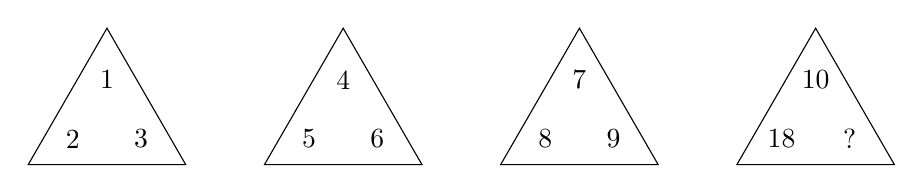
\begin{tikzpicture}[scale=1.0]
      % \begin{scope}[shift={(0,0)}]
      %   \coordinate(A) at (0,0);
      %   \coordinate(B) at (2,0);
      %   \coordinate(C) at (60:2);
      %   \coordinate(O) at ($1/3*(A)+1/3*(B)+1/3*(C)$);
      %   \draw(A)--(B)--(C)--cycle;
      %   \node at ($(90:.5)+(O)$) {1};
      %   \node at ($(210:.5)+(O)$) {2};
      %   \node at ($(330:.5)+(O)$) {3};
      % \end{scope}

      \begin{scope}[shift={(3,0)}]
        \coordinate(A) at (0,0);
        \coordinate(B) at (2,0);
        \coordinate(C) at (60:2);
        \coordinate(O) at ($1/3*(A)+1/3*(B)+1/3*(C)$);
        \draw(A)--(B)--(C)--cycle;
        \node at ($(90:.5)+(O)$) {1};
        \node at ($(210:.5)+(O)$) {2};
        \node at ($(330:.5)+(O)$) {3};
      \end{scope}

      \begin{scope}[shift={(6,0)}]
        \coordinate(A) at (0,0);
        \coordinate(B) at (2,0);
        \coordinate(C) at (60:2);
        \coordinate(O) at ($1/3*(A)+1/3*(B)+1/3*(C)$);
        \draw(A)--(B)--(C)--cycle;
        \node at ($(90:.5)+(O)$) {4};
        \node at ($(210:.5)+(O)$) {5};
        \node at ($(330:.5)+(O)$) {6};
      \end{scope}

      \begin{scope}[shift={(9,0)}]
        \coordinate(A) at (0,0);
        \coordinate(B) at (2,0);
        \coordinate(C) at (60:2);
        \coordinate(O) at ($1/3*(A)+1/3*(B)+1/3*(C)$);
        \draw(A)--(B)--(C)--cycle;
        \node at ($(90:.5)+(O)$) {7};
        \node at ($(210:.5)+(O)$) {8};
        \node at ($(330:.5)+(O)$) {9};
      \end{scope}
      
      \begin{scope}[shift={(12,0)}]
        \coordinate(A) at (0,0);
        \coordinate(B) at (2,0);
        \coordinate(C) at (60:2);
        \coordinate(O) at ($1/3*(A)+1/3*(B)+1/3*(C)$);
        \draw(A)--(B)--(C)--cycle;
        \node at ($(90:.5)+(O)$) {10};
        \node at ($(210:.5)+(O)$) {18};
        \node at ($(330:.5)+(O)$) {?};
      \end{scope}
    \end{tikzpicture}
  \end{center}
  \begin{align*}
    (\mathrm{A})\ 200 \quad\quad (\mathrm{B})\ 600 \quad\quad (\mathrm{C})\ 800\quad\quad (\mathrm{D})\ 1200
  \end{align*}
\end{example}
\begin{proof}[提示]平方和的数字和,直到最后是一位数。
  \begin{align*}
    &1^2+2^2+3^2 = 14, && \implies 1 + 4 = 5\\
    &4^2+5^2+6^2 = 74, && \implies 7 + 4 = 14, && \implies 1+4=5\\
    &7^2+8^2+9^2 = 194,&& \implies 1+9+4=14, && \implies 1+4=5
  \end{align*}
  按这个规律,?号处填200,最后会得到5。
\end{proof}

\chapter{数论}
\label{chap:number-theory}

\epigraph{Die ganzen Zahlen hat der liebe Gott gemacht, alles andere ist Menschenwerk.\\
  上帝创造了自然数,其余的都是人的工作。}{Leopold Kronecker(利奥波德·克罗内克)}

Kronecker是德国数学家与逻辑学家,主要研究代数和数论,特别是在椭圆函数理论上有突出贡献。以克罗内克命名的数学理论包括克罗内克$\delta$函数、克罗内克积等。

\section{自然数}
\label{sec:what-is-natural-number}

关于自然数(Natural Number)所指,目前并没有定论,有时是指正整数$1,2,3,\cdots$,有时是指非负整数$0,1,2,3,\cdots$,取决于主观意愿。在这里,为避免混淆,只采用正整数、非负整数等无疑义的说法。

\section{质数}
\label{sec:prime-number}

\begin{definition}[质数,Prime Number]
  一个大于$1$的正整数,若除了$1$和它本身之外没有其它的因子,则称该数为质数,也叫素数。不是质数的正整数称为合数。
\end{definition}

\begin{table}[htbp]
  \centering
  \begin{tabular}{cccccccccc}
    \hline
    2  & 3  & 5  & 7  & 11 & 13 & 17 & 19 & 23 & 29\\
    31 & 37 & 41 & 43 & 47 & 53 & 59 & 61 & 67 & 71\\
    73 & 79 & 83 & 89 & 97 &    &    &    &    &   \\
    \hline
  \end{tabular}
  \caption{100以内的质数}
  \label{tab:prime-numbers<100}
\end{table}

\begin{property}
  $2$是唯一的一个偶数质数。
\end{property}

\begin{theorem}
  有无穷多个质数。
\end{theorem}
\begin{proof}
  下面是欧拉提出的方法,用反证。假设只有有限个质数$p_1,p_2,\cdots,p_n$,那么对于正整数$p_{n+1}=p_1p_2p_3\cdots p_n + 1$,显然有$p_{n+1}$不被$p_1,p_2,\cdots,p_n$整除,从而找到一个$p_1,p_2,\cdots,p_n$之外且比它们都大的质数$p_{n+1}$,矛盾。
\end{proof}

可以用欧拉的反证法构造质数数列。从质数数列$p_1,p_2,\cdots,p_n$出发,则$p_1p_2\cdots p_n+1$要不是质数,要不就含有一个不同于$p_1,p_2,\cdots,p_n$的质因子,从而可找到下一个质数$p_{n+1}$。

\begin{example}
  从$41$出发,按欧拉方法找出$5$个不同的质数。
\end{example}
\begin{proof}[解]千万不要用纸笔算,除非你想锻炼计算能力,请利用计算机编程验证,让合适的人做合适的事。
  \begin{align*}
    p_1 & = 41 && p_1 + 1 = 42 = 2\times 3\times 7&&\text{随便取一个,比如取2}\\
    p_2 & = 2  && p_1p_2 + 1 = 2\times41 + 1=83   &&\text{是质数}\\
    p_3 & = 83 && p_1p_2p_3 + 1=6807=3\times2269  &&\text{为方便起见,取3}\\
    p_4 & = 3  && p_1p_2p_3p_4+1=20419=7\times2917&&\text{取7}\\
    p_5 & = 7  &&                                 &&\qedhere
  \end{align*}
\end{proof}

下面是除了著名的哥德巴赫猜想(参考例~\ref{ex:Goldbach-conjecture})之外的又一个关于质数的悬而未决的猜想。
\begin{example}[成对质数的猜想]
  以$p$与$p+2$形式成对出现的质数有无穷多个。
\end{example}
\begin{proof}[示例]
  如$(3,5)$、$(11,13)$、$(17,19)$、$(29,31)$和$(41,43)$等等都是这种成对形式的质数。
\end{proof}

\section{整除}
\label{sec:divisible}

\begin{definition}
  若整数$a$是整数$b$的整数倍,即存在某个整数$q$,使得$a=bq$,则称$b$整除$a$,也称$a$被$b$整除。记为$b\mid a$。$b$不能整除$a$则记为$b\notdivides a$。
\end{definition}

\begin{example}
  \begin{align*}
    17293\mid 0,\quad 4\mid 28,\quad 5\notdivides 12
  \end{align*}
\end{example}

\subsection{最大公约数}
\label{sec:gcd}

\begin{definition}[最大公约数,Greatest Common Divisor(gcd)]
  两个不同时为零的整数$a,b$的公约数中最大的一个称为$a,b$的最大公约数,记为$\gcd(a,b)$。
\end{definition}

\begin{example}
  \begin{align*}
    \gcd(0,8)=8,\quad 
    \gcd(-9,-12)=\gcd(9,12)=3,\quad
    \gcd(7,22)=1
  \end{align*}
\end{example}

\begin{definition}[互质,Coprime]
  若$\gcd(a,b)=1$,则称$a,b$互质。
\end{definition}
$\gcd(a,b)=1$是指$a,b$除了$1$之外没有其余的正的公约数。

\begin{theorem}
  若$a,b$互质,且质数$p\mid ab$,则必有$p\mid a$或者$p\mid b$。
\end{theorem}
\begin{corollary}
  若$a_1,a_2,\cdots,a_n$两两互质,且质数$p\mid a_1a_2\cdots a_n$,则$p$必能整除$a_1,a_2,\cdots, a_n$中的某一个。
\end{corollary}

\begin{example}
  $4,5,9$两两互质,其乘积为$4\times5\times9=180$,作质因式分解,有
  \begin{align*}
    180=2^2\times 3^2\times 5
  \end{align*}
  从而能整除$180$的质数只有$2,3,5$,这三个数都能整除$4,5,9$中的某一个。
\end{example}

\begin{theorem}
  若整数$a,b$互质,且$b\mid ac$,则必有$b\mid c.$
\end{theorem}

\begin{definition}[欧拉函数,Euler Function]\label{def:Euler-function}
  对于任意正整数$n$,欧拉函数$\varphi(n)$表示从$1$到$n$中与$n$互质的整数的个数。
\end{definition}

\begin{table}[htbp]
  \centering
  \begin{tabular}{cccccccccccccccc}
    \toprule
    $n$          & 1 & 2 & 3 & 4 & 5 & 6 & 7 & 8 & 9 & 10 & 11 & 12 & 13 & 14 & $\cdots$\\\midrule
    $\varphi(n)$ & 1 & 1 & 2 & 2 & 4 & 2 & 6 & 4 & 6 & 4  & 10 & 4  & 12 & 6  & $\cdots$\\
    \bottomrule
  \end{tabular}
  \caption{欧拉函数表}
  \label{tab:Euler-function-values}
\end{table}

\begin{theorem}
  若正整数$n$是质数,则$\varphi(n)=n-1$,若正整数$n$是合数,且其质因数分解式为
  \begin{align*}
    n=p_1^{a_1} p_2^{a_2} p_3^{a_3} \cdots p_k^{a_k}
  \end{align*}
  其中$p_1,p_2,p_3,\cdots,p_k$是互不相等的质数,则
  \begin{align*}
    \varphi(n)=n\left(1-\frac1{p_1}\right) \left(1-\frac1{p_2}\right) \left(1-\frac1{p_3}\right) \cdots \left(1-\frac1{p_k}\right)
  \end{align*}
\end{theorem}

\begin{example}[求$\varphi(15)$]
  由于$15=3\times 5$,在$1,2,3,\cdots,15$中,不是$3$的倍数的占$1-1/3=2/3$,不是$5$的倍数的占$1-1/5=4/5$。
  \begin{align*}\setlength\arraycolsep{3pt}\renewcommand*{\arraystretch}{.9}
    \begin{array}{cccccccccccccccc}
                         & 1 & 2 & 3 & 4 & 5 & 6 & 7 & 8 & 9 & 10 & 11 & 12 & 13 & 14 & 15\\
    \text{排除$3x$}\quad & 1 & 2 & \cancel3 & 4 & 5 & \cancel6 & 7 & 8 & \cancel9 & 10 & 11 & \cancel{12} & 13 & 14 & \cancel{15}\\
    \text{排除$5x$}\quad & 1 & 2 & 3 & 4 & \xcancel5 & 6 & 7 & 8 & 9 & \xcancel{10} & 11 & 12 & 13 & 14 & \xcancel{15}
    \end{array}
  \end{align*}
  从而
  \begin{align*}
    \varphi(15)=15\times\left(1-\frac13\right)\times\left(1-\frac15\right)
    =15\times\frac23\times\frac45=8
  \end{align*}
\end{example}

\begin{definition}[非负整数系数线性组合]
  给定$x_1, x_2, \cdots, x_n$,对任意非负整数$a_1,a_2,\cdots, a_n$,称
  \begin{align*}
    a_1 x_1 + a_2 x_2 + \cdots + a_3 x_n
  \end{align*}
  为$x_1, x_2, \cdots, x_n$的非负整数系数线性组合。
\end{definition}

\begin{example}[硬币问题,Frobenius coin problem]
  给定若干种面额的硬币,每种面额的硬币数量足够多,那么用这些硬币所不能表达的最大的整数价值是多少?如用$2$元和$5$元的硬币,所不能表示的整数价值有$1$元、$3$元;偶数都可以用若干$2$元的表示,大于或等于$5$的奇数都可以用一个$5$以及若干个$2$表示,从而$3$就是$2,5$的非负整数系数线性组合里不包含的最大整数。

  Frobenius硬币问题的数学提法如下:

  给定正整数$a_1, a_2, \cdots, a_n$且$\gcd(a_1, a_2, \cdots, a_n)=1$,求这些正整数的非负整数系数线性组合所不包含的整数的最大值。这个最大整数就称为$a_1, a_2,\cdots, a_n$的Frobenius Number,通常记为$g(a_1,a_2,\cdots, a_n)$。
\end{example}

\begin{example}[麦乐鸡鸡块问题,McNugget Numbers]
  $80$年代时,英国的麦当劳售卖三种规格的麦乐鸡块盒,每种盒子里分别有$6,9,20$块鸡块。有些数量的鸡块能通过购买三种鸡块盒得到,有些数量则不可以。问不能通过购买这三种鸡块盒得到的鸡块数量的最大值是什么?
\end{example}

\begin{theorem}
  若正整数$m,n$互质,则$m,n$的非负整数系数线性组合所不包含的正整数的个数为
  \begin{align*}
    \dfrac{(m-1)(n-1)}2
  \end{align*}
  且其Frobenius数$g(m,n)=mn-m-n$。
\end{theorem}
\begin{proof}下面简称能被$m,n$的非负整数系数线性组合所表示的正整数为可表示的,否则称为不可表示的。
  
  首先证明任意整数$k\ge mn-m-n+1=(m-1)(n-1)$是可表示的。可由定理~\ref{th:Skupien}的证明可得。亦可利用贝祖定理~\ref{th:Bezout}及二元一次不定方程的理论得到,引用的地方比较多,看看就好。由$m,n$互质及贝祖定理,存在整数$a,b$使得$ma+nb=1$。从而$m\times(ak)+n\times(bk)=k$。从而对于关于$x,y$的二元一次不定方程$mx+ny=k$的所有整数解为$x=ak+tn, y=bk-tm$,其中$t$是任意整数。选择$t$,使得$x\in[0,n-1)$,则对于此$t$,有
  \begin{align*}
    &mx + ny = k > mn -m -n \\
    \implies\quad& n(y+1)>m(n-1-x)>0\\
    % \overset{x\in[0,n-1)}{\implies}\quad&
                                            \implies\quad&y+1>0\\
    \implies\quad& y\ge0    
  \end{align*}
  从而此$t$使得$x,y$均非负且满足$mx+ny=k$,即$k$可表示。


  其次证明$mn-m-n\equiv (m-1)(n-1)-1$是不可表示的。反证。假设存在非负整数$x,y$,使得
  \begin{align*}
    mn-m-n=mx+ny
  \end{align*}
  两边分别对$m,n$取模,则有
  \begin{align*}
    \begin{cases}
      -n&\equiv ny\pmod m\\
      -m&\equiv mx\pmod n
    \end{cases}
    \underset{m,n\text{互质}}{\implies}
    \begin{cases}
      y\equiv -1\equiv m-1 \pmod m\\
      x\equiv -1\equiv n-1 \pmod n
    \end{cases}
  \end{align*}
  再由$x,y$的非负性,有$y\ge m-1, x\ge n-1$,从而
  \begin{align*}
    mx + ny\ge m(n-1) + n(m-1) = 2mn -m -n > mn - m -n
  \end{align*}
  矛盾。从而$mn-m-n$不可表示。

  最后证明不可表示的正整数个数为$(m-1)(n-1)/2$。这需要用到以下事实:对于任意的整数$k\in[0,g(m,n)]$,$(k, g(m,n)-k)$这两个数中总是只有一个能被表示。由于两个可表示的数之和是可表示的,而$k + g(m,n)-k = g(m,n)$是不可表示的,从而$(k,g(m,n)-k)$这两数中最多只有一个是可表示的,从而至少有一个是不可表示的。设$k$是不可表示的,剩余需要证明$g(m,n)-k$是可表示的,从而两个只恰好有一个是可表示的一个是不可表示的。由前面证明所述,关于$x,y$的二元一次不定方程$mx+ny=k$的所有解都可以表示为$x=a+tn,y=b-tm$,选择$t$,使得$x\in[0,n-1)$。由于$k$是不可表示的,从而此$t$对应的$y<0\implies y\le-1$,否则$x,y$非负,$k=mx+ny$可表示。因此有
  \begin{align*}
    g(m,n)-k=mn-m-n-mx-my=m(n-1-x)+n(-y-1)
  \end{align*}
  由$x\in[0,n-1)$及$y\le -1$可知$n-1-x\ge0, -y-1\ge0$,从而$g(m,n)-k$可表示。

  结合起来,有$g(m,n)=(m-1)(n-1)$,且不可被表示的正整数有$k/2=(m-1)(n-1)/2$个。。
\end{proof}

\begin{theorem}[Skupi\'en的推广]\label{th:Skupien}
  若正整数$m,n$互质,则对任意正整数$k \ge (m-1)(n-1)$,存在唯一的非负整数$\alpha,\beta$,使得$\alpha < n$且$k =\alpha m + \beta n$。
\end{theorem}
\begin{proof}
  存在性。由定理~\ref{th:coprime-modular},$\{im: 0\le i< n\}=\{0,m,2m,\cdots,(n-1)m\}$这$n$个数模$n$两两不同余,故对任意整数$k\ge (m-1)(n-1)$,$k,k-m,k-2m,k-3m,\cdots,k-(n-1)m$模$n$两两不同余,从而其中某一个模$n$为$0$,不妨记$k-\alpha m\equiv 0\pmod n$,其中$0\le \alpha \le n-1$,从而存在整数$\beta$,使得$k-\alpha m = \beta n$,即$k=\alpha m + \beta n$。

  非负性。
  由上面构造方法,已有$0\le\alpha<n$,且$\beta n = k-\alpha m\ge (m-1)(n-1)-(n-1)m=1-n$,从而$(\beta+1)n\ge1\implies\beta\ge0$。

  唯一性。给定$k\ge (m-1)(n-1)$,若存在非负整数$\alpha<n,a<n$及非负整数$\beta, b$,使得$k=\alpha m + \beta n = am + bn$,则$(\alpha -a)m=(b-\beta)n$,由$m,n$互质,可知$m\mid b-\beta, n\mid\alpha -a$。但$\alpha<n, a<n$,从而$-n<\alpha-a<n$,从而只有$\alpha = a$才能有$n\mid \alpha -a$,继而$\beta = b$。
\end{proof}

\subsection{最小公倍数}
\label{sec:lcm}

\begin{definition}[最小公倍数,Least Common Multiple(lcm)]
  两个非零整数$a,b$的正的公倍数中最小的一个称为$a,b$的最小公倍数,记为$\lcm(a,b)$。
\end{definition}

\begin{example}
  \begin{align*}
    \lcm(3,7)=21,\quad \lcm(4,6)=12,\quad \lcm(-6,9)=\lcm(6,9)=18
  \end{align*}
\end{example}

\begin{theorem}
  任意两个非零整数$a,b$,有$\gcd(a,b)\cdot\lcm(a,b)=ab.$
\end{theorem}
\begin{proof}[提示]
  记$s\equiv ab/\gcd(a,b)$,则首先$s$是$a,b$的公约数,其次用反证法证明$s$是$a,b$所有正公约数中最小的一个,从而$s=\lcm(a,b)$。
\end{proof}

\section{同余}
\label{sec:modular}

\begin{example}[模5同余]
  一个整数被$5$除时,余数只能是$0,1,2,3,4$这$5$种之一。可以把所有的整数按除$5$的余数分类,则可分为$5$类:
  \begin{align*}\renewcommand*{\arraystretch}{.9}\setlength\arraycolsep{4pt}
    \begin{array}{cccccccccc}
      \text{第1类,余数为0:} & \quad \cdots, & -15, & -10, & -5, & 0, & 5, & 10, & 15, & \cdots\\
      \text{第2类,余数为1:} & \quad \cdots, & -14, & -9,  & -4, & 1, & 6, & 11, & 16, & \cdots\\
      \text{第3类,余数为2:} & \quad \cdots, & -13, & -8,  & -3, & 2, & 7, & 12, & 17, & \cdots\\
      \text{第4类,余数为3:} & \quad \cdots, & -12, & -7,  & -2, & 3, & 8, & 13, & 18, & \cdots\\
      \text{第5类,余数为4:} & \quad \cdots, & -11, & -6,  & -1, & 4, & 9, & 14, & 19, & \cdots
    \end{array}
  \end{align*}
  每一类中任意两数都称为模$5$同余。
\end{example}

类似的,对任意整数$d$,可得到模$d$同余的概念。容易得到,以下关于两整数$a$和$b$模$d$同余的定义是等价的:
\begin{enumerate}
\item $a$、$b$模$d$的余数相同;
\item $a-b$能被$d$整除;
\item 存在某个整数$n$使得$a=b+nd$。
\end{enumerate}

一般使用高斯所创记法表示同余关系,即用
\begin{align*}
  a \equiv b \pmod d \quad\quad a\not\equiv b\pmod d
\end{align*}
分别表示$a$和$b$模$d$同余、$a$和$b$模$d$不同余。

\subsection{整除的性质}
\begin{example}[被$7$整除]\label{ex:divided-by-7}
  任意一个整数$n$,可以唯一地用若干个正整数$a_i$表示为
  \begin{align*}
    n=\sum_{i=0}^{k} a_i\times 10^i
  \end{align*}
  其中$0\le a_i<10$,如
  \begin{align*}
    32568 = 8 + 6\times 10 + 5\times 10^2 + 2\times 10^3 + 3\times10^4
  \end{align*}
  观察$10^i$模$7$的余数,可得表~\ref{tab:10^i-modular-7}。

  \begin{table}[htbp]
    \centering
    \begin{tabular}{cccccccccc}
      \toprule
                & $10^0$ & $10^1$ & $10^2$ & $10^3$ & $10^4$ & $10^5$ & $10^6$ & $10^7$ & $\cdots$ \\ \midrule
      模$7$余数 & $1$    & $3$    & $2$    & $6$    & $4$    & $5$    & $1$    & $3$    & $\cdots$ \\ 
      \bottomrule
    \end{tabular}
    \caption{$10^i$模$7$余数}
    \label{tab:10^i-modular-7}
  \end{table}

  由于$10\not\equiv0\pmod7$,所以$10^i$模$7$的余数永不为零,表格中只会出现$1,2,3,4,5,6$这$6$个余数,且每$6$个一循环。从而
  \begin{align*}
    n\equiv\,&\sum_{i=0}^{k} a_i\times10^i\tag*{$\pmod7$}\\
     \equiv\,& a_0\times10^0 + a_1\times10^1 + a_2\times10^2 + a_3\times10^3 + a_4\times10^4 + a_5\times10^5 +\\
             & a_6\times10^6 + a_7\times10^7 + a_8\times10^8 + \cdots \tag*{$\pmod7$}\\
     \equiv\,& a_0 + 3a_1 + 2a_2 + 6a_3 + 4a_4 + 5a_5 +\\
             & a_6 + 3a_7 + 2a_8 + 6a_9 + \cdots\tag*{$\pmod7$}
  \end{align*}
  所以若$n=\sum\limits_{i=0}a_i\times10^i$能被$7$整除,当且仅当
  $a_0 + 3a_1 + 2a_2 + 6a_3 + 4a_4 + 5a_5 + a_6 + 3a_7 + 2a_8 + 6a_9 + \cdots$
  能被$7$整除。
\end{example}

\begin{example}
  整数$782370456$能否被$7$整除?
\end{example}
\begin{proof}[提示]
  将大于$7$的数字减去$7$,原数能否被$7$整除等价于$012300456=12300456$能否被$7$整除。按下面表格
  \begin{align*}\renewcommand{\arraystretch}{.9}
    \begin{array}{ccccccccc}
      \toprule
      i                    & 0 & 1 & 2 & 3 & 4 & 5 & 6 & 7\\ \midrule
      \text{数字倒序}      & 6 & 5 & 4 & 0 & 0 & 3 & 2 & 1\\
      \text{$10^i$模7余数} & 1 & 3 & 2 & 6 & 4 & 5 & 1 & 3\\
      \bottomrule
    \end{array}
  \end{align*}
  将上下两行对应数字相乘并求和,则原数能否被$7$整除等价于$6\times1 + 5\times3 + 4\times2 + 0\times6 +0\times4 + 3\times5 + 2\times1 + 1\times3 = 49$能否被$7$整除。
\end{proof}

\begin{question}[被3或9整除]
  用类似的方式,证明一个正整数若能被$3$(或$9$)整除,等价于其数字之和能被$3$(或$9$)整除。
\end{question}
\begin{proof}[提示]
  任意非负整数$i$,有$10^i\equiv 1\pmod3$,$10^i\equiv1\pmod9$。
\end{proof}

\begin{theorem}\label{th:coprime-modular}
  若正整数$a,b$互质,则$0,a,2a,3a,\cdots,(b-1)a$模$b$两两不同余。
\end{theorem}
\begin{proof}
  反证。否则存在$0\le i<j$,使得$ia\equiv ja\pmod b$,从而$b\mid (j-i)a > 0$,而$j-i<b$,从而有$j-i$与$b$互质,因而有$b\mid a$,这与$a,b$互质矛盾。
\end{proof}

\subsection{同余的运算}
\label{sec:op-of-modular}

在例~\ref{ex:divided-by-7}中用到了同余式的以下性质。若$a\equiv\alpha\pmod d, b\equiv\beta\pmod d$,则对任意整数$u,v$,有
\begin{enumerate}
\item $au+bv\equiv \alpha u+\beta v\pmod d$;
\item $ab\equiv \alpha\beta\pmod d$;
% \item $u^a\equiv u^{\alpha}\pmod d$;
\item $a^u\equiv \alpha^{u}\pmod d$。
\end{enumerate}

%% 其实由第2条性质可以直接得到第3条,取$b=a,\beta=\alpha$代入,有$a^2\equiv\alpha^2\pmod d$,然后取$a\to a^2,\alpha\to\alpha^2,b=a,\beta=\alpha$代入,又有$a^3\equiv\alpha^3\pmod d$,依次类推。

注意,$u^a\equiv u^{\alpha}\pmod d$则不一定成立,如$2\equiv9\pmod7$,但取$u=3$,则$3^2\equiv2\not\equiv6\equiv 3^9\pmod7$。

\begin{question}
  求$12\times88\times43\times1988$模$7$的余数。
\end{question}
\begin{proof}[提示]
  \begin{align*}\renewcommand{\arraystretch}{.9}\setlength\arraycolsep{2pt}
    \begin{array}{ccccccccl}
             & 12 & \times & 88 & \times & 43 & \times & 1989 &\\
      \equiv & 5  & \times & 11 & \times & 1  & \times & 1212 &\quad\pmod7\\
      \equiv & 5  & \times & 4  & \times & 1  & \times & 512  &\quad\pmod7\\
      \equiv & 5  & \times & 4  & \times & 1  & \times & 22   &\quad\pmod7\\
      \equiv & 5  & \times & 4  & \times & 1  & \times & 1    &\quad\pmod7
    \end{array}
  \end{align*}
  上述变化中,$88\to 11, 1989\to1212$是将每个大于7的数字减7;$11\to4$是整体减7;$1212\to512,512\to22$是将最前面的几位(这里是两位)减去7的倍数,分别是$12-7=5, 51-49=2$。
\end{proof}

\subsection{费马小定理}
\label{sec:Fermat-theorem}

\begin{theorem}[费马小定理,Fermat's Little Theorem]
  给定质数$p$,则对任意的正整数$a$,有$a^p\equiv a\pmod p$;若$p\notdivides a$,则同时有$a^{p-1}\equiv1\pmod p$。
\end{theorem}
\begin{proof}
  若$p|a$,即$a\equiv0\pmod p$,则显然有$a^p\equiv a\equiv0\pmod p$。

  对于$a\notdivides p$,考虑$a,2a,3a,\cdots,(p-1)a$这$p-1$个数。可以证明其中任意两个不模$p$不同余,否则两个的差$(s-t)a$能被$p$整除,其中$1\le s<t\le p-1$不能被$p$整除,再由$p$是质数从而必须有$a$被$p$整除,矛盾。于是在模$p$同余下,这$p-1$个数必与$1,2,3,\cdots,p-1$重新排列后一一对应,从而有
  \begin{align*}
    & a \times 2a \times 3a \times \cdots \times (p-1)a
    \equiv 1 \times 2 \times 3 \times \cdots \times (p-1) \pmod p\\
    \implies & (1\times 2\times 3\times\cdots\times (p-1))(a^{p-1}-1)\equiv0\pmod p
  \end{align*}
  由于$p$不能整除$1,2,3,\cdots,p-1$中任意一个,且$p$为质数,从而$p$整除$a^{p-1}-1$,即$a^{p-1}\equiv1\pmod p$,从而也有$a^p\equiv a\pmod p$。
\end{proof}

\begin{corollary}
  若正整数$a,b$互质,则$a^{\varphi(b)}\equiv1\pmod b$,其中$\varphi$是\ref{def:Euler-function}中的欧拉函数。
\end{corollary}


\subsection{辗转相除法}
\label{sec:Euclidean-algorithm}

\begin{theorem}\label{th:euclidean-algorithm-theorem}
  若整数$a,b,q,r$满足$a=bq+r$,即$a\equiv r\pmod b$,则$\gcd(a,b)=\gcd(b,r).$
\end{theorem}
\begin{proof}[提示]
  任意同时整除$a,b$的数同时也能整除$r$;反之,任意同时整除$b,r$的数同时也能整除$a$。
\end{proof}

\begin{definition}[辗转相除法]
  对任意两正整数$a,b$,求$\gcd(a,b)$。若$a=b$,则$\gcd(a,b)=\gcd(a,a)=a$。下面不妨设$a>b$,从而由定理~\ref{th:euclidean-algorithm-theorem},有
  \begin{align*}
    a&=  \,bq_1 + r_1,   &&\quad(0\le r_1 < b)   & \gcd(a,b)    &=\,\gcd(b,r)\\
    b&=  \,r_1q_2 + r_2, &&\quad(0\le r_2 < r_1) & \gcd(b,r_1)  &=\,\gcd(r_1, r_2)\\ 
    r_1&=\,r_2q_3 + r_3, &&\quad(0\le r_3 < r_2) & \gcd(r_1,r_2)&=\,\gcd(r_2, r_3)\\
    r_2&=\,r_3q_4 + r_4, &&\quad(0\le r_4 < r_3) & \gcd(r_2,r_3)&=\,\gcd(r_3, r_4)\\
    \multicolumn{7}{c}{$\cdots$}\\
    r_{n-1}&=\,r_nq_{n+1} + 0, &&\quad(0\le r_n < r_{n-1}) & \gcd(r_{n-1},r_n)&=\,\gcd(r_{n}, 0)=r_{n}
  \end{align*}
  由于$r_i$每次总要减小,所以在有限个步骤后总有某个$r_{n+1}=0$,此时可得$\gcd(a,b)=r_n.$
\end{definition}

\begin{example}
  求$\gcd(1234,678).$
\end{example}
\begin{proof}[提示]在辗转相除法求$\gcd$中,商$q_i$是没有用的,利用计算机中的取模运算\%,可以方便的得到
  \begin{align*}\renewcommand{\arraystretch}{.9}\setlength{\arraycolsep}{2pt}
    \begin{array}{ccccc}
      1234 & \% & 678 & = & 556\\
      678  & \% & 556 & = & 122\\
      556  & \% & 122 & = & 68\\
      122  & \% & 68  & = & 54\\
      68   & \% & 54  & = & 14\\
      54   & \% & 14  & = & 12\\
      14   & \% & 12  & = & 2\\
      12   & \% & \textcircled{2}   & = & 0
    \end{array}
  \end{align*}
  所以$\gcd(1234,678)=2$。
\end{proof}

\section{整数分类}
\label{sec:category}

按不同的分类方法,整数可以分为不同的集合。按同余分类是一种比较常见的分类方法,如按模$2$的余数分类,可分为奇数和偶数。再比如在研究幻方中则通常将幻方(参考\ref{chap:magic-square})的阶数按$2n+1, 4n, 4n+2$的形式来分类。

\begin{example}
  将正整数分成若干子集,使得任意正整数$x$与$2x$不在同一个子集内。则最少只需要两个子集。
\end{example}
\begin{proof}
  按大小顺序依次安放各数,奇数可以随便放,因其不是任意整数的两倍。放偶数$n$时,只要放入$n/2$所在的另一个子集即可。

  另一种方法,任意正整数可以唯一地写为$2^km$的形式,其中$m$是正奇数,$k$是非负整数。若$n_1=2^{k_1}m_1 = 2n_2=2\cdot 2^{k_2}m_2$,则$k_1=k_2+1$其奇偶性不同。将正整数按上述分解中$k$的奇偶性分成两类,每类作一个子集即可。
\end{proof}

\section{重要定理}
\label{sec:important-thorems-of-number-theory}



\chapter{连分数}
\label{chap:continued-fraction}

\section{定义}
\label{sec:definition-of-continued-fraction}

\begin{definition}
  对于正整数$a_0, a_1, a_2, \cdots, a_n$,以下形式的有理数称为连分数:
  \begin{align*}
    a_0 + \dfrac1{a_1 + \dfrac1{a_2 + \dfrac1{\ddots + \dfrac1{a_n}}}}
  \end{align*}
\end{definition}

利用\ref{sec:Euclidean-algorithm}中的欧拉辗转相除法,可以将一个有理数转化为连分数。

\begin{example}
  将$324/138$化为连分数的形式。
  \begin{align*}
    324 = 138\times2 + 48 &\quad\implies\quad \frac{324}{138} = 2 + \dfrac{48}{138} = 2 + \dfrac1{\dfrac{138}{48}}\\
    138 = 48\times 2 + 42 &\quad\implies\quad \frac{324}{138} = 2 + \dfrac{1}{2 + \dfrac{42}{48}} = 2 + \dfrac{1}{2 + \dfrac1{\dfrac{48}{42}}}\\
    48 = 42\times1 + 6 & \quad\implies\quad \frac{324}{138} = 2 + \dfrac{1}{2 + \dfrac1{1 + \dfrac{6}{42}}} =  2 + \dfrac{1}{2 + \dfrac1{1 + \dfrac1{\dfrac{42}{6}}}}\\
    42 = 6\times7 + 0 &  \quad\implies\quad \frac{324}{138} = 2 + \dfrac{1}{2 + \dfrac1{1 + \dfrac1{7}}}
  \end{align*}
\end{example}


\chapter{不定方程}
\label{chap:diophantine-equation}

\epigraph{三人同行七十稀,五树梅花廿一支,\\七子团圆正半月,除百零五便得知。}{明·程大位《算法统宗》}

一般来说,求解$n$个未知变量,需要$n$个条件。
不定方程是指约束个数少于未知数个数的方程(组)。由于约束少,不定方程通常有无穷多的解。

这里只讨论整数系数不定方程的整数解问题。早在三世纪初,古希腊数学家丢番图(Diophantus)就研究过若干此类方程,所以不定方程也称为丢番图方程(Diophantine equation)。

\section{线性不定方程}
\label{sec:linear-diophantine-equation}

\begin{theorem}
  若$\gcd(a,b)\notdivides c$,则不定方程$ax+by=c$无整数解。
\end{theorem}
\begin{proof}
  反证。假设存在整数解$x=x_0, y=y_0$,由于存在整数$a_0,b_0$满足$a=a_0\cdot\gcd(a,b), b=b_0\cdot\gcd(a,b)$,从而有
  \begin{align*}
    &c=a_0\cdot\gcd(a,b)x_0 + b_0\cdot\gcd(a,b)y_0=\gcd(a,b)(a_0x_0+b_0y_0)
  \end{align*}
  从而有$\gcd(a,b)\mid c$,矛盾。
\end{proof}

\begin{theorem}
  若不定方程$ax+by=c$有一个整数解$x_0, y_0$,则不定方程的通解(指所有整数解)为
  \begin{align*}
    \begin{cases}
      x=x_0+k\cdot\gcd(a,b)\\
      y=y_0-k\cdot\gcd(a,b)
    \end{cases}, \quad k\in\mathcal{Z}
  \end{align*}
\end{theorem}
\begin{proof}
  首先容易验证$x=x_0+kb, y=y_0-ka$是不定方程的整数解。其次,对不定方程的任一整数解$x=x', y=y'$,由
  \begin{align*}
    ax_0 + by_0 =c, \quad ax' + by' =c
  \end{align*}
  两式相减,则有$a(x_0-x')=b(y'-y_0)$。记$a_0=a/\gcd(a,b), b_0=b/\gcd(a,b)$,则$a_0,b_0$互质,且有$a_0(x_0-x')=b_0(y'-y_0)$,从而$a_0\mid y'-y_0$,从而存在整数$k$,使得$y'-y_0=ka_0$,代入可分别求得$x'=x_0-kb_0, y'=y_0+ka_0$。

  由此定理,要求不定方程的通解,只需找到一组特解即可。
\end{proof}

\begin{example}
  求不定方程$4x+6y=14$的所有整数解。
\end{example}
\begin{proof}[提示]
  首先原不定方程化简为$2x+3y=7$,其系数为$2,3$,由$\gcd(2,3)=1\mid 7$,原不定方程有整数解。将方程变形,有
  \begin{align*}
    2x = 7-3y,\quad\implies\quad x=\frac{7-3y}{2}=3-y+\frac{1-y}{2}
  \end{align*}
  为使$x$是整数,取$y=1$,则$x=2$,此即为特解。其通解按公式可得。
\end{proof}

\begin{example}
  求不定方程$7x+19y=283$的所有整数解。
\end{example}
\begin{proof}[提示]
  首先$\gcd(7,19)=1$,所以有整数解。变换形式如下
  \begin{align*}
    x=\frac{283-19y}{7}=40+\frac{3-19y}{7}=40+\frac{3-21y+2y}{7}=40-3y+\frac{3+2y}{7}
  \end{align*}
  用$y=1,2,3,\cdots$枚举,试出$7\mid 3+2y$的某个$y$。
  \begin{center}
    \begin{tabular}{cccccccccc}
      \toprule
      $y$    & 1 & 2 & 3 & 4  & 5  & 6  & 7  & 8  & 9 \\
      $3+2y$ & 5 & \textcircled{7} & 9 & 11 & 13 & 15 & 17 & 19 & \textcircled{21}\\
      \bottomrule
    \end{tabular}
  \end{center}
  取$y=2$,使$x=40-3*2+1=35$,此即为特解。  
\end{proof}

\section{猴子分果}
\label{sec:monkeys-dividing-fruits}

\begin{example}
  5只猴子去采果子,采完后把果子放到一起,由于太累了便都呼呼大睡了。

  后来,1只猴子先醒来,把果子平均分成5份后发现多了一个,于是它把多的一个扔了,从剩下的5份里拿了一份走了。

  第2只猴子醒了,把剩余的果子平均分成了5份,发现多了2个,于是它把多的2个也扔了,从剩下的5份里拿了一份走了。

  第3只猴子醒了,把剩余的果子平均分成了5份,发现多了3个,于是它把多的3个也扔了,从剩下的5份里拿了一份走了。

  第4只猴子醒了,把剩余的果子平均分成了5份,发现多了4个,于是它把多的4个也扔了,从剩下的5份里拿了一份走了。

  第5只猴子醒了,把剩余的果子平均分成了5份,发现不多不少,它从剩下的5份里拿了一份走了。

  问这些猴子共采了多少个果子?
\end{example}
\begin{proof}
  可以列出不定方程组。记第$i$个猴子拿走了$x_i$个果子,则有
  \begin{align*}
    4x_1 &= 5x_2 + 2, & 4x_2 &= 5x_3 + 3\\
    4x_3 &= 5x_4 + 4, & 4x_4 &= 5x_5
  \end{align*}
  于是总共采到的果子数$s$为
  \begin{align*}
    s&=5x_1 + 1 \\
     &=5\times\frac14 (5x_2+2) + 1 = \frac{25}{4}x_2 + \frac72\\
     &=\frac{25}{4}\times \frac14\times (5x_3+3) + \frac72 = \frac{125}{16}x_3 + \frac{131}{16}\\
     &=\frac{125}{16}\times \frac14 (5x_4+4) + \frac{131}{16} = \frac{625}{64}x_4 + 16\\
     &=\frac{625}{64}\times \frac14\times5x_5 + 16 = \frac{5^5x_5}{4^4} + 16
  \end{align*}
  由于$\gcd(5,4)=1$,从而要使$s$是整数,必有整数$k$,使得$x_5=4^4k$,即$s=5^5k + 16$,且此时有
  \begin{align*}
    x_5& = 4^4 k,&\quad x_4&=\frac54\times 4^4k = 5\times4^3k \\
    x_3&=\frac14(5x_4+4) = 5^2\times4^2k + 1,&\quad x_2 &= \frac14(5x_3+3) = 5^3\times 4k + 2\\
    x_1&=\frac14(5x_2 + 2) = 5^4k + 3
  \end{align*}
  从而猴子们采摘的果子总数可能为
  \begin{align*}
    k&=0 \implies\  s= 5^5\times0 + 16=16\\
    k&=1 \implies\  s= 5^5\times1 + 16=3141\\
    k&=2 \implies\  s= 5^5\times2 + 16=6266&&\qedhere
  \end{align*}
\end{proof}

\begin{example}
  这是丢番图提的一个问题:求三个数,使它们的和及其中任意两数之和都是完全平方数。
\end{example}
\begin{proof}
  丢番图给出过一个解:$(80,320,41)$。实际上这个问题是有无穷多的整数解的。
\end{proof}


\section{的士数}
\label{sec:taxicab-number}

1919年,哈代(Godfrey Harold Hardy)前往看望病重的拉马努金(Srinivasa Ramanujan)。哈代说:“我乘的士来,车牌号码是1729。这个数可真没趣,希望不是不祥之兆。”拉马努金回答说:“不,那是个有趣得很的数。可以用两个立方数之和来表达而且有两种表达方式的数中,1729是最小的。”

\begin{definition}[的士数,Taxicab number]
  能以$n$个不同的方法表示成两个正立方数之和的最小的正整数称为第$n$个的士数,通常记为$\mathrm{Ta}(n)$。
\end{definition}

对于$\mathrm{Ta}(2)$,它实际上是不定方程$x^3+y^3=u^3+v^3$的一个正整数解的立方和。到上前为止,只找到前6个的士数。前三个如表~\ref{tab:taxicab-number}所示。$\mathrm{Ta}(4)$、$\mathrm{Ta}(5)$和$\mathrm{Ta}(6)$过于复杂,此处不列出。
\begin{table}[htbp]
  \centering
  \begin{tabular}{cl}
    \toprule
    $n$              & \multicolumn{1}{c}{$\mathrm{Ta}(n)$}\\\midrule
    1                & $2 = 1^3 + 1^3$\\
    2                & $1729=1^3+12^3=9^3+10^3$\\
    3                & $87539319=167^3+436^3=228^3+423^3=255^3+414^3$\\
    \bottomrule
  \end{tabular}
  \caption{的士数}
  \label{tab:taxicab-number}
\end{table}

\section{中国剩余定理}
\label{sec:Chinese-remainder-theorem}

\begin{definition}[模反元素,Modular multiplicative inverse]
  整数$a,b,m$若满足$ab\equiv1\pmod m$,则称$a,b$是模$m$的模反元素。
\end{definition}

\begin{theorem}[模反的存在性]
  若$a,m$互质,则存在$a$模$m$的模反元素。
\end{theorem}
\begin{proof}[提示]
  考虑$a,2a,3a,\cdots,ma$这$m$个数,由于$a,m$互质,它们模$m$是两两不同余的,否则两个同余的相减会导出$m\mid a$的矛盾。而模$m$的同余类只有$m$个,从而其中必有一个模$m$等于1。
\end{proof}

\begin{example}
  南北朝·孙子《孙子算经》:今有物不知其数,三三数之余二,五五数之余三,七七数之余二。问物有几何?
\end{example}
\begin{proof}[提示]
  与二元线性不方程类似,只要找到一组特解$x$,则所有的整数解都可以表达为$x+t\cdot\lcm(3,5,7)=x+105t$。

  三人同行七十稀。对$3,5,7$,先找一个数$a$,满足$a\equiv 1\pmod3, a\equiv0\pmod5, a\equiv0\pmod7$,由后两个,有$a=5\cdot7\cdot x$,取$x$为$5\cdot 7$为模$3$的模反元素,即$35x\equiv1\pmod3$,可取$x=2$,此时$a=70$。

  五树梅花廿一枝。对$3,5,7$,找一个数$b$,满足$b\equiv0\pmod3, b\equiv1\pmod5,b\equiv0\pmod7$,由模3模7为0,有$b=21y$,取$y$为21模5的模反元素,即$21y\equiv1\pmod5$,可取$y=1$,此时$b=21$。

  七子团圆正半月。对$3,5,7$,找一个数$c$,满足$b\equiv0\pmod3, b\equiv0\pmod5,b\equiv1\pmod7$,由模3模5为0,有$c=15z$,取$z$为15模7的模反元素,即$15z\equiv1\pmod7$,可取$z=1$,此时$c=15$。

  由此可得到一个特解$2\times 70+3\times 21+2\times 15=233$。其所有正整数解为$23,128,233,338,\cdots$。
\end{proof}

\begin{theorem}[孙子定理,中国剩余定理,Chinese remaider theorem]
  大于$1$的正整数$n_1,n_2,\cdots, n_k$两两互质,则对任意整数$a_1,a_2,\cdots,a_k$,方程组
  \begin{align*}
    x\equiv&\ a_1\pmod{n_1}\\
    x\equiv&\ a_2\pmod{n_2}\\
    &\cdots\\
    x\equiv&\ a_k\pmod{n_k}
  \end{align*}
  有正整数解。  
\end{theorem}
\begin{proof}
  用构造方法找出一组特解。取定下标$i$,构造数$x_i$,使得
  \begin{align*}
    \begin{cases}
      x_i\equiv1\pmod{n_i}\\
      x_i\equiv0\pmod{n_j}, \quad\forall j\ne i
    \end{cases}
  \end{align*}
  由后一个条件,$x_i$为如下形式
  \begin{align*}
    x_i=t_i\cdot \underbrace{n_1n_2\cdots n_{i-1}n_{i+1}\cdots n_k}_{\text{没有}n_i}=t_i\cdot \frac{n_1n_2 \cdots n_k}{n_i}
  \end{align*}
  记$M_i\equiv\dfrac{n_1n_2\cdots n_k}{n_i}$,取$t_i$为$M_i$模$n_i$的模反元素(由于$n_i,M_i$互质,$t_i$是存在的),则$x_i=t_iM_i$满足条件。

  对所有下标$i$,构造出$x_i$后,可得一个特解
  \begin{align*}
    x=a_1x_1+a_2x_2+\cdots+a_kx_k&\qedhere
  \end{align*}
\end{proof}

\begin{theorem}
  记$x$是剩余问题的一个特解,则其整数通解为$x+t\cdot n_1n_2\cdots n_k$.
\end{theorem}
\begin{proof}
  设$y$是剩余问题的任一整数解,考虑$y-x$,则对任意下标$i$,有$y-x\equiv0\pmod{n_i}$,而$n_1,n_2,\cdots,n_k$两两互质,从而存在整数$t$,使得$y-x=t\cdot n_1n_2\cdots n_k$。
\end{proof}



\chapter{历法}
\label{chap:calendar}

\epigraph{清明时节雨纷纷,路上行人欲断魂。\\借问酒家何处有,牧童遥指杏花村。}{唐·杜牧《清明》}

清明是中国从古流传至今的二十四节气之一,而公历是近代才传入中国的,为什么每年的清明不是公历4月4日就是4月5日呢?

\section{太阳历}
\label{sec:solar-calendars}

太阳历又称为阳历,是以地球绕太阳公转的运动周期为基础而制定的历法。

\begin{definition}[回归年,太阳年,Tropical Year,Solar Year]
  太阳年是指在地球上观察到太阳回到同一个地方所需要的时间,即地球绕太阳旋转一周所需要的时间,大约是$365.2422$天。
\end{definition}

由于太阳年不是整数,而历年都是整数天数,所以通常为的历法都是在历年中插入天数来调整。在太阳历中,平年有365天,大约每隔4年就要添加一日(闰日),该年就是有366天的闰年。儒略历(Julian Calendar)就采用这种置闰方式。

按儒略历每4年一闰日,日历上过了4年为$1+365\times4$天,而实际的4个太阳年共有$365.2422\times4$天,从而4年下来其误差为$1+365\times4-365.2422\times4=1-0.2422\times4=0.0312$天,再扩大一下,日历上过了400年,则与实际的400个太阳年误差为3.12天,即比太阳年多跑了3.12天。为解决这个误差,格里历(Gregorian Calendar),即现在通用的公历,在每400年中去掉3个闰年。格里历的置闰规则如下:
\begin{quotation}
  四年一闰,百年不闰,四百年再闰。
\end{quotation}

剩余的每400年产生的$3.12-3=0.12$天的误差,就需要后人在用到时继续修正了。

\begin{definition}[闰年,Leap Year]
  2月份有28天的称为平年,2月份有29天的称为闰年。确定平年闰年的方法是:
  \begin{enumerate}
  \item 能被400整除的年份定为闰年;
  \item 否则能被100整除的年份定为平年;
  \item 否则能被4整除的年份定为闰年;
  \item 其余年份定为平年。
  \end{enumerate}
  即不能被4整除的都是平年;能被400整除的是闰年;不能被400整除但能被100整除的是平年;不能被100整除但能被4整除的是闰年。
\end{definition}

闰年置闰日的方法是在当年2月份增加一天,从原来的28天加到29天。

\begin{table}[htbp]
  \centering
  \begin{minipage}{\textwidth}  %for footnote in tabular
  \begin{tabular}{ccccccccccccc}
    \toprule
    月份 & 1  & 2          & 3  & 4  & 5  & 6  & 7  & 8  & 9  & 10 & 11 & 12\\\midrule
    天数 & 31 & 28\footnote{平年28天,闰年29天} & 31 & 30 & 31 & 30 & 31 & 31 & 30 & 31 & 30 & 31\\
    \bottomrule
  \end{tabular}
  \end{minipage}
\caption{每月天数}
  \label{tab:days-of-months}
\end{table}

\begin{example}
  公元1900年是平年,因为$400\notdivides 1900$,且$100\mid 1900$。公元2012年是闰年,因为$4\mid 2012$且$100\notdivides 2012$。
\end{example}

\begin{example}
  小明已经上小学4年级了,可是他却说:“我妈妈说我每个生日都没有落下,可是我到现在为止总共才给我过了3个生日。”小明说的有可能吗?
\end{example}
\begin{proof}[提示]
  比如闰年闰日过生日。
\end{proof}

\begin{example}[10年3650天]
  陈奕迅有首歌叫《十年》,吕珊有首歌叫《3650夜》。那么,十年到底有可能是几天?
\end{example}
\begin{proof}[提示]
  普通情况下,四年一闰。考虑到百年不闰的情况,十年有可能有一个闰年、两个闰年或三个闰年。
  \begin{align*}
    \cdots,\underline{2008},2009,2010,2011,\underline{2012},2013,2014,2015,\underline{2016},2017,2018,2019,\underline{2020},\cdots
  \end{align*}
  从2008--2017这十年包含了3个闰年(下划线部分),从2009--2018这十年包含了两个闰年。考虑百年不闰的1900年,以其为中心向两边扩散,则十年范围可只包含一个闰年。
  \begin{align*}
    1897,1898,1899,1900,1901,1902,1903,\underline{1904},1905,1906&\qedhere
  \end{align*}
\end{proof}

\begin{example}
  小明是2013年入学的小学生,今年全家去旅行,过了三天后回家。到家后小明一连撕掉了3张日历。姨妈打电话过来问起小明什么时候去的旅行,小明说不记得了,只记得刚刚撕掉的3张日历的数字和是32。那么你知道小明旅行是在哪一年吗?
\end{example}
\begin{proof}[提示]
  撕掉3张日历,暗示了这3张正好对应小明旅行的3天日期。两种情况,一是3天都是同一月份,二是3天在不同的月份。

  如果3天是同一月份,则连续3天的日期之和应能被3整除,然而32并不能被3整除,排除这种情况。

  3天不在同一月份,则必须有一天是上月月末,一天是当月月初一号,另外一天可能是当月2号,也可能是上月倒数第二天。如果是上月月末一天外加当月一号二号两天,则上月月末日期数字为$32-1-2=29$。如果是当月一号外加上月最后两天,则上月最后两天的日期数字之和为$32-1=31$,不可能,因为每月最后两天日期数字之和最小的也有$27+28>31$。所以被撕掉的3天日期的唯一情况是$29,1,2$。

  从而当年是闰年。从2013年开始的闰年按顺序依次为:2016,2020,2024,$\cdots\cdots$。而小明是2013年上的小学,题目中说明全家旅行时小明仍然是小学生。如果是2020年的2月份去的旅行,那么小明在旅行时应该已经是初中二年级上学期了,所以题目中说的今年只能是2016年。
\end{proof}


\section{太阴历}
\label{sec:tai-yin-calendar}



\section{大明历}
\label{sec:da-ming-calendar}

祖冲之在公元465(也有人说是公元462年,即刘宋大明六年)制定了大明历。祖冲之在此之前就测得了地球围绕太阳旋转一周的天数大约为365.24281481天。由于该数不是正整数,古人制定历法,很重要的一件事情就是对历法调整安排,使得制定的历法与季节的循环相匹配。

\section{节气}
\label{sec:jie-qi}

古人把$360^\circ$黄经划分24等分,每隔$15^\circ$为一节气,其中$0^\circ$为春分,夏至是$90^\circ$,秋分是$180^\circ$,冬至是$270^\circ$。而太阳黄经在$15^\circ$时则定为清明,太阳直射北回归线之日即中国北方最热之时定为夏至,如图~\ref{fig:24-jie-qi}所示。

公历(即格里历)是根据太阳年来确定,其日期是与黄经基本是一一对应的,误差在一日之内(闰日),所以黄经每个角度对应的公历日期基本是固定的,所以节气在公历上的体现也基本是固定的,误差也在一日之内。

\begin{figure}[htbp]
  \centering
  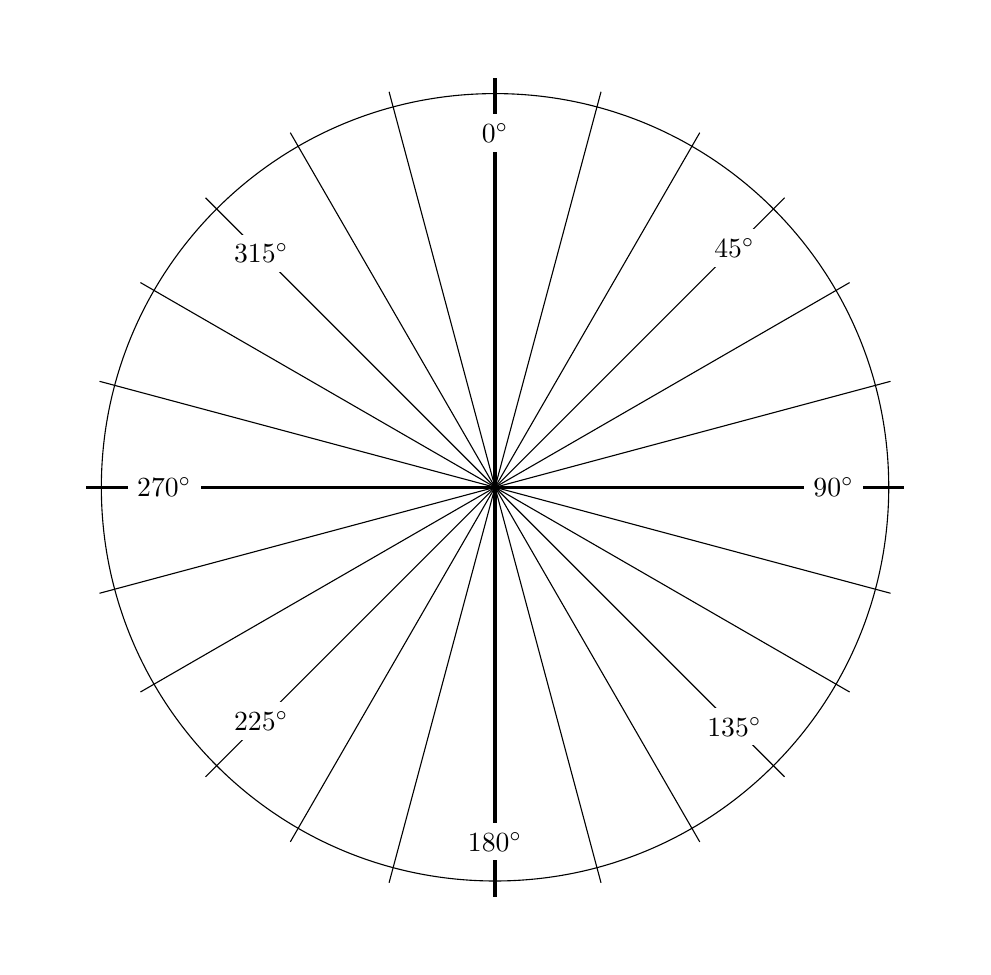
\begin{tikzpicture}[scale=1.0]
    \draw(0,0)circle(5);
    \foreach \a/\v in {0/春分,15/清明,30/谷雨,45/立夏,60/小满,75/芒种,90/夏至,
      105/小暑,120/大暑,135/立秋,150/处暑,165/白露,180/秋分,
      195/寒露,210/霜降,225/立冬,240/小雪,255/大雪,270/冬至,
      285/小寒,300/大寒,315/立春,330/雨水,345/惊蛰
    }{
      \draw(0,0)--(90-\a:5.2)node[pos=1.1]{\v};
    }
    \foreach \a/\r/\v in {0/4.5/$0^\circ$, 90/4.3/$90^\circ$, 180/4.5/$180^\circ$, 270/4.2/$270^\circ$}{
      \draw[very thick](0,0)--(90-\a:5.2);
      \node[fill=white] at(90-\a:\r) {\v};
    }
    \foreach \a/\r/\v in {45/4.3/$45^\circ$, 135/4.3/$135^\circ$, 225/4.2/$225^\circ$, 315/4.2/$315^\circ$}{
      % \draw[very thick](0,0)--(90-\a:5.2);
      \node[fill=white] at(90-\a:\r) {\v};
    }
  \end{tikzpicture}
  \caption{二十四节气}
  \label{fig:24-jie-qi}
\end{figure}

节气是古人用于指导工作的,如春耕、播种等,与太阳与地球的相对位置密切相关的。节气实际上是一种阳历。即中国古代所使用的历法既包括阴历,也包括阳历(节气),所以实际上是一种阴阳历。

\chapter{黄金比例}
\label{ch:golden-ratio}


\section{定义}
\label{sec:golden-ration-defition}

\begin{definition}
  将线段分为长短两截,若短的一截比长的一截等于长的一截比原线段的长度,则此分割为\term{黄金分割}。
\end{definition}

\begin{center}
  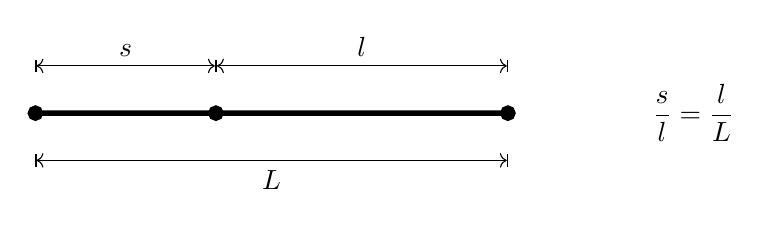
\begin{tikzpicture}[scale=6.0]
    \draw[line width=2pt,fill=black](0,0)circle(.3pt)--(.382,0) circle(.3pt)--(1,0)circle(.3pt);
    \draw[|<->|](0,.1)--(0.382,.1)node[midway,above]{$s$};
    \draw[|<->|](1,.1)--(0.382,.1)node[midway,above]{$l$};
    \draw[|<->|](0,-.1)--(1.000,-.1)node[midway,below]{$L$};
    \node[left] at(1.5,0) {$\dfrac{s}{l}=\dfrac{l}{L}$};
  \end{tikzpicture}
\end{center}

记原线段长度为L,在黄金分割下,长一截长度为$l$,短的一截长度为$s$,则
\begin{align*}
  \frac sl=\frac l{l+s} \quad\implies \frac sl = \frac1{1+\dfrac sl}\quad\implies
  \left(\frac sl\right)^2 + \frac sl = 1
\end{align*}
再加上条件$s<l$,从而有
\begin{align*}
  \frac ls=\frac{\sqrt5+1}2\approx 1.618, \quad \frac sl=\frac{\sqrt5-1}2\approx 0.618
\end{align*}
以上两个常数都称为\term{黄金比例},通常用$\phi$和$\Phi$表示,即
\begin{align*}
  \phi\equiv\frac{\sqrt5+1}2,\quad \Phi\equiv\frac{\sqrt5-1}2
\end{align*}


\section{性质}
\label{sec:golden-ration-properties}

\begin{question}
  证明下列恒等式:
  \begin{align*}
    \phi\cdot\Phi=1,\quad \phi=\Phi+1,\quad \phi^2=\phi+1,\quad \frac1\phi=\phi-1
  \end{align*}
\end{question}

\begin{example}[连分数表示]\label{ex:phi-of-continued-fraction}
  \begin{align}
    \phi = 1 + \dfrac1{1 + \dfrac1{1+\dfrac1{1+\dfrac1{1+\cdots}}}}
  \end{align}
\end{example}
\begin{proof}
  利用$\phi=1+\dfrac1\phi$,设连分数为$x$,则
  \begin{align*}
    \frac1{x-1}=x\implies x^2-x-1=0\implies x=\frac{1\pm\sqrt5}2
  \end{align*}
  由$x>0$可知$x=\dfrac{1+\sqrt5}2=\phi$。
\end{proof}

\begin{definition}
  以下数值称为\term{贵金属分割}:
  \begin{align}
    \frac{n+\sqrt{n^2+4}}2,\quad\quad n=1,2,3,\cdots
  \end{align}
  当$n=1$时为黄金分割$\dfrac{\sqrt5+1}2$;当$n=2$时为\term{白银分割}$\sqrt2+1$;当$n=3$时为\term{青铜分割}$\dfrac{\sqrt{13}+3}2$。
\end{definition}
\begin{question}
  证明:贵金属分割都可以用以下的连分数形式表示
  \begin{align*}
    \frac{n+\sqrt{n^2+4}}2=
    n+\dfrac1{n+\dfrac1{n+\dfrac1{n+\dfrac1{n+\dfrac1{n+\cdots}}}}}
  \end{align*}
\end{question}

\begin{example}[平方根表示]
  \begin{align}
    \phi=\sqrt{1+\sqrt{1+\sqrt{1+\sqrt{1+\sqrt{1+\cdots}}}}}
  \end{align}
\end{example}
\begin{proof}
  记等号右边为$x$,则$x^2 = 1 + x$,余下与题~\ref{ex:phi-of-continued-fraction}相同,略。
\end{proof}

\begin{example}[三角函数表示]
  $\phi=1 + 2\sin18^\circ.$
\end{example}
\begin{proof}
  由$\phi=1+\Phi$,等价于证明$2\sin18^\circ=\Phi$。令$x\equiv18^\circ$,则$2x+3x=5x=90^\circ=\frac\pi2$,应用以下公式
  \begin{align*}
    \sin 2x &= \cos \left(\frac\pi2 - 2x\right) = \cos 3x\\
    \sin 2x &=2\sin x\cos x\\
    \cos 3x &= 4\cos^3x-3\cos x
  \end{align*}
  可得
  \begin{align*}
    &2\sin x\cos x = 4\cos^3x-3\cos x\\
    \implies& \cos x(2\sin x - 4\cos^2 x + 3) = 0  & (cos x\ne 0)\\
    %\overset{\cos x\ne 0}{\implies} & 2\sin x + 4\sin^2 x - 1 = 0
    \implies & 2\sin x + 4\sin^2 x - 1 = 0 
  \end{align*}
  从而有
  \begin{align*}
    \sin x = \dfrac{-2\pm\sqrt{20}}{8}=\dfrac{-1\pm\sqrt5}4
  \end{align*}
又$x=18^\circ$,显然$\sin x>0$,从而有
\begin{align*}
  \sin18^\circ&=\sin x =\dfrac{\sqrt5-1}4=\dfrac\Phi2\qedhere
\end{align*}
\end{proof}

\begin{example}[黄金长方形]
  长宽比满足黄金比例的长方形称为\term{黄金长方形},如下图。\par
  \begin{center}
    \begin{tikzpicture}[scale=2.5];
      \draw(0,0)rectangle($({.5*(sqrt(5)+1)},1)$);
    \end{tikzpicture}
  \end{center}
\end{example}

\begin{example}[尺规作图]
  找出线段$AB$的黄金分割点。
\end{example}
关键点在于作出$\sqrt5$的长度,作出一个边长分别为$1,2,\sqrt5$的直角三角形。这里取$AB$的长度为$2$,则
\begin{enumerate}
\item 找出$AB$的中点$O$,则$AO=BO=1$;
\item 以$AO$为长度在过点$B$的$AB$垂直线上找点$C$,使$BC=AO=1$,则$AC=\sqrt5$;
\item 在$AC$上找点$D$,使$DC=BC=1$,此时$AD=\sqrt5-1$;
\item 在$AB$上找点$S$,使$AS=AD=\sqrt5-1$,从而$\dfrac{AS}{AB}=\dfrac{\sqrt5-1}{2}$,即点$S$是$AB$的黄金分割点。
\end{enumerate}
% \begin{figure}[htbp]
\begin{center}
  % \centering%\fbox{
  \vspace*{-5cm}
  \begin{tikzpicture}[scale=3]
    \coordinate[label=below left:$A$] (A) at (0,0);
    \coordinate[label=below right:$B$] (B) at (2,0);
    \coordinate[label=above:$C$] (C) at (2,1);
    \coordinate (O) at (1,0);
    \tkzInterLC(A,C)(C,B)\tkzGetPoints{D}{};
    \tkzInterLC(A,B)(A,D)\tkzGetPoints{}{S}\tkzLabelPoints[below](O,S)
    \calcLength(A,D){AD}
    %\draw(S) arc(0:40:\AD pt);
    \tkzMarkRightAngle[color=blue](A,B,C)
    \drawArc(A,S,D)
    \draw(A)--(O) node[midway,sloped]{||} -- (B)--(C) node[midway,sloped]{||}--(D)node[midway,sloped]{||} --cycle;
    % \draw(B) arc(270:200:1);
    \drawArc(C,B,D);
    \tkzDrawPoints(A,B,C,O,D,S);

    \clip(-1,0)rectangle(3,1);
  \end{tikzpicture}
%}
\end{center}
%   \caption{黄金分割的尺规作图}
%   \label{fig:golden-ratio-of-ruler-and-compass-construction}
% \end{figure}

\begin{definition}
  腰与底边的长度比是$\phi$的等腰三角形称为\term{黄金三角形}。
\end{definition}
\note 有时把腰与底边的长度比是$\Phi$的等腰三角形也称为黄金三角形。但此处只考虑比值是$\phi$的情况,即腰比底长的等腰三角形。


\begin{definition}
  等腰三角形的一条底角平分线将三角形分为两个三角形,若含底边的小三角形与原三角形相似,则称原三角形为\term{黄金三角形}。
\begin{center}
    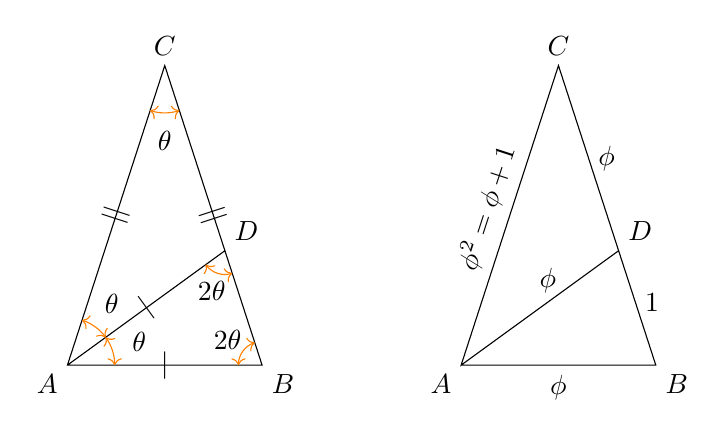
\begin{tikzpicture}[scale=1];
      \begin{scope}[shift={(0,0)}]
        \coordinate(A) at (0,0);
        \coordinate(C) at (72:4);
        \coordinate(B) at ($(C)!1!36:(A)$); %rotate A to 36 degree around C
        \tkzDefLine[bisector](C,A,B)\tkzGetPoint{D'}
        \tkzInterLL(A,D')(B,C)\tkzGetPoint{D}
        \draw(A)--(B)node[midway,sloped]{|}--(C)node[midway,sloped]{||}--cycle node[midway,sloped]{||}--(D)node[midway,sloped]{|};
        \draw pic["$\theta$",<->,draw=orange,angle eccentricity=1.6,angle radius=.6cm]{angle=D--A--C};
        \draw pic["$\theta$",<->,draw=orange,angle eccentricity=1.6,angle radius=.6cm]{angle=B--A--D};
        \draw pic["$\theta$",<->,draw=orange,angle eccentricity=1.6,angle radius=.6cm]{angle=A--C--B};
        \draw pic["$2\theta$",<->,draw=orange,angle eccentricity=1.8,angle radius=.3cm]{angle=C--B--A};
        \draw pic["$2\theta$",<->,draw=orange,angle eccentricity=1.8,angle radius=.3cm]{angle=A--D--B};
        \tkzLabelPoints[below left](A)
        \tkzLabelPoints[below right](B)
        \tkzLabelPoints[above](C)
        \tkzLabelPoints[above right](D)
      \end{scope}
      \begin{scope}[shift={(5,0)}]
        \coordinate(A) at (0,0);
        \coordinate(C) at (72:4);
        \coordinate(B) at ($(C)!1!36:(A)$); %rotate A to 36 degree around C
        \tkzDefLine[bisector](C,A,B)\tkzGetPoint{D'}
        \tkzInterLL(A,D')(B,C)\tkzGetPoint{D}
        \draw(A)--(B)node[midway,sloped,below]{$\phi$}
                --(D)node[pos=.55,right]{$1$}
                --(C)node[midway,right]{$\phi$}
                --(A)node[midway,sloped,above]{$\phi^2=\phi+1$}
                --(D)node[pos=.55,above]{$\phi$};
        \tkzLabelPoints[below left](A)
        \tkzLabelPoints[below right](B)
        \tkzLabelPoints[above](C)
        \tkzLabelPoints[above right](D)
      \end{scope}
    \end{tikzpicture}
  \end{center}
\end{definition}

\begin{theorem}
  一个等腰三角形是黄金三角形的充要条件是其顶角是$\dfrac\pi5(36^\circ)$。
\end{theorem}
\begin{proof}
  必要性:由图,$5\theta=\pi$,从而$\theta=\dfrac\pi5$。

  充分性:若等腰三角形顶角$\angle C=\dfrac\pi5$,则容易计算到到$\angle BAD=\dfrac\pi5$,从而$\triangle ABC\sim\triangle BAD$,即$\triangle ABC$是黄金三角形。
\end{proof}

\begin{question}
  证明黄金三角形各边长度的比例关系如上图所示。
\end{question}

\begin{question}
  证明正五角星(Regular Pentagram)的顶点可组成黄金三角形。
  \begin{center}
    
\begin{tikzpicture}[scale=.6]
      \coordinate(A) at ( 18:4);
      \coordinate(B) at ( 90:4);
      \coordinate(C) at (162:4);
      \coordinate(D) at (234:4);
      \coordinate(E) at (306:4);
      \draw(A)--(C)--(E)--(B)--(D)--cycle;
    \end{tikzpicture}
  \end{center}
\end{question}

\begin{example}[数值逼近]
  $\phi$是方程$x^2-x-1=0$的一个解,应用牛顿迭代法(Newton's method)逐渐逼近$\phi$。
\end{example}

选择初始点$x_0=3$,利用牛顿迭代公式(参考第~\pageref{sec:Newton-method}~页~\ref{sec:Newton-method}~节)
\begin{align*}
  x_{n+1}=x_n-\frac{f(x_n)}{f'(x_n)}=x_n-\frac{x_n^2-x_n-1}{2x^n-1}=\frac{x_n^2+1}{2x^n-1}
\end{align*}
从而有
\begin{align*}
  x_0&=3 &
  x_1&=2\\
  x_2&=1.66666666666667 &
  x_3&=1.61904761904762\\
  x_4&=1.61803444782168 &
  x_5&=1.61803398874999\\
  x_6&=1.61803398874989 &
  x_7&=1.61803398874989
\end{align*}
可以看出已经开始向$\phi$收敛,在上述保留14位小数的精度下迭代到$x_7$已经不变了。牛顿迭代法特别适合于应用计算机对方程求数值近似解。

\chapter{技巧}
\label{chap:tricks}

\section{代数}
\label{tricks-of-algebra}

\begin{example}
  证明:
  \begin{align*}
    \frac{a}{b+c} + \frac{b}{c+a} + \frac{c}{a+b} = 1 \quad \implies\quad
    \frac{a^2}{b+c} + \frac{b^2}{c+a} + \frac{c^2}{a+b} = 0
  \end{align*}
\end{example}
\begin{proof}[提示]
  两边同乘$a+b+c$,有
  \begin{align*}
    (a+b+c)\left(\frac{a}{b+c} + \frac{b}{c+a} + \frac{c}{a+b}\right) = a+b+c
  \end{align*}
  且若$a+b+c\ne 0$,则左右两式是等价的。
\end{proof}


\chapter{数值方法}
\label{chap:numerical-method}

数值方法通常是指应用计算机程序求解数值问题的近似解的各种方法与工具。

其中常见的是迭代法,即不断地用旧值递推出新值的过程。比如数论中的辗转相除法也是一种迭代方法。

\section{迭代法}
\label{sec:iteration-method}

\subsection{韦达跳跃}
\label{sec:vieta-jumping}

韦达跳跃(Vieta Jumping)的其中一种方法,是利用韦达定理构造新点,从而问题跳转到新获得的点上。

\begin{example}[Putnam 1988]
  证明:对于任意正整数$N$,方程
  \begin{align*}
    x_1^2+x_2^2+x_3^2+x_4^2=x_1x_2x_3+x_2x_3x_4+x_3x_4x_1 + x_4x_1x_2
  \end{align*}
  总有$x_1,x_2,x_3$和$x_4$全大于$N$的整数解。
\end{example}
\begin{proof}[提示]用迭代法,从一个特殊解开始不断地构造更大的解。首先猜一个正整数解$(x_1,x_2,x_3,x_4)=(a_1,a_2,a_3,a_4)$。容易猜出来$(x_1,x_2,x_3,x_4)=(1,1,1,1)$是一个正整数解。

  其次,从$(a_1,a_2,a_3,a_4)$出发,构造另一组更大的整数解。由对称性,不妨假设$a_1\le a_2\le a_3\le a_4$。保持较大的$a_2,a_3,a_4$不动,若将$a_1$换成一个比$a_4$大的正整数$a_5$且$(a_2,a_3,a_4,a_5)$满足方程的话,则$\left(a_2, a_3,a_4, a_5\right)$就是另一组更大的解,且有
  $a_1\le a_2\le a_3\le a_4 < a_5$。用同样的方式,可以找到$a_6, a_7, a_8, \cdots$,使得序列
  \begin{align*}
    a_1\le a_2\le a_3\le a_4 < a_5 < a_6 < a_7 < a_8 < \cdots
  \end{align*}
  中连续的四项为原方程的一组解。

  下面考虑得到另一个解。对于$x_1$,原方程是一个二元方程,$a_1$是其中一个解,则由韦达定理可得到另一个关于$x_1$的解。变换形式如下:
  \begin{align*}
    x_1^2 - (x_2x_3+x_3x_4+x_4x_2)x_1 + x_2^2 + x_3^2 + x_4^2 - x_2x_3x_4=0
  \end{align*}
  关于$x_1$的方程的两个根$u, v$应满足
  \begin{align*}
    u + v = x_2x_3+x_3x_4+x_4x_2
  \end{align*}
  把其中一个根$x_1=a_1$及系数$x_2=a_2, x_3=a_3, x_4=a_4$代入,则有另一个根(记为$a_5$)为
  \begin{align*}
    a_5 = a_2a_3 + a_3a_4 + a_4a_2 - a_1
  \end{align*}
  又显然有$a_5  \ge a_3a_4 + a_4a_2 > a_4$,从而按此公式,可得到序列的下一项。

  总结如下。开始项:$(1,1,1,1)$,下一项的递推公式为
  \begin{align*}
    a_n = %f(a_{n-1},a_{n-2},a_{n-3},a_{n-4}) =
    a_{n-1}a_{n-2} + a_{n-2}a_{n-3} + a_{n-3}a_{n-1} - a_{n-4}
  \end{align*}
  这种苦力,用计算机容易得到下面的结果:
  \begin{align*}
    1,1,1,1,2, 4, 8, 16, 32, 64, 128, 256, 512, 1024, 2048,\cdots
  \end{align*}
  更进一步地,由上面这个结果,还能得到什么更有趣的结果?
\end{proof}

\begin{example}[IMO 1988]
  $a,b$是正整数,且$ab + 1|a^2+b^2$,证明$\frac{a^2+b^2}{ab+1}$是完全平方数。
\end{example}
\begin{proof}[提示]
  这是一道非常有名的题目。即使是当年的金牌获得者,13岁的陶哲轩(Terrence Tao,最年轻的金牌获得者,后面于2006年获得了fields medal)在此题上也只是拿到了7分中的1分。当时只有11名学生完美地解决了这个问题。

  用韦达跳跃及反证,即从最小的$(a,b)$出发,通过韦达跳跃跳到一个比$(a,b)$更小的点上,从而导致矛盾。

  \begin{enumerate}
  \item 记 $S\equiv \{(a,b)|a,b\text{是正整数且}\dfrac{a^2+b^2}{ab+1}\text{是正整数但不是完全平方数}\}$。
  \item 若$S$非空,找出其中一个$(A,B)$使得$A+B$最小,即记$(A,B)\in S$,且有$\forall (a,b)\in S$,有
    \begin{align*}
      A + B \le a + b
    \end{align*}
    由对称性不妨设$A\ge B$。下面由韦达跳跃找到一个更小的来导出矛盾。
  \item 固定$B$,若能找到$C$,使$(B,C)\in S$且$C<A$,则$B+C<A+B$与$(A,B)$的定义矛盾。设$k = \frac{A^2+B^2}{AB+1}$,若同时有$k = \frac{C^2+B^2}{CB+1}$,则$A,C$都是以下方程的解:
    \begin{align*}
      \frac{x^2 + B^2}{Bx + 1} = 0 \implies x^2 - kxB + B^2 - k = 0
    \end{align*}
    即若$A,C$是这个方程的角,则由韦达定理,有
    \begin{align*}
      C = kB - A, \quad\text{且}\quad C = \frac{B^2 - k}{A}
    \end{align*}

  \item 由$C=kB - A$知$C$是整数;由$C = \frac{B^2 - k}{A}$且$k$不是完全平方数知$C\ne 0$;再由$\frac{C^2 + B^2}{CB + 1}=k>0 \implies CB+1>0 \implies C>0$。从而$C$是正整数,且$(C,B)\in S$且$C+B = \frac{B^2-k}{A} + B < A + B$。
  \end{enumerate}
  由此矛盾可知$S$中不存在最小的$(A,B)$,从而$S$只能是空集。
\end{proof}


\section{牛顿法}
\label{sec:Newton-method}

牛顿法是一种迭代方法。迭代方法的思想是通过一个初始点,不断地迭代得到一系列的点,而这些点序列最终会收敛到目标点上。具体来说,牛顿法是通过曲线的切线来构造下一个点,因而牛顿法通常也叫做切线法。

\begin{enumerate}
\item 从一个初始点$(x_0, 0)$开始,找到曲线上的点$(x_0, f(x_0))$;
\item 作切线,找到切线与$x$轴的交点$(x_1,0)$;
\item 从$(x_1,0)$开始重复上述步骤
\end{enumerate}

按上述步骤,可得到一系列的值$x_0, x_1, x_2, \cdots, $。在某些条件下,$x_i$会收敛到曲线与$x$轴的交点。其递推关系为
\begin{align*}
  x_{n+1}=x_0 - \frac{f(x_0)}{f'(x_0)}
\end{align*}
上述迭代的不动点(即迭代完了之后还是它本身),在$f'$不为零的情况下等价于$f(x)$的零点。这是因为
\begin{align*}
  x=x-\frac{f(x)}{f'(x)} \quad \overset{f'\ne0}{\iff}\quad f(x)=0
\end{align*}

\begin{theorem}
  若函数$f(x)$在$x=\alpha$处为零,即$f(\alpha)=0$,且$f(x)$有连续的导数,且$f'(\alpha)\ne0$。则存在$x=\alpha$的一个邻域,在此邻域内任意一点$x_0$出发按牛顿切线法得出的点序列$\{x_i\}$收敛于$\alpha$。
\end{theorem}
由此定理可知,有连续导数的函数的零点如果其导数不会零,则该零点有一个吸引域,在此吸引域内的点按牛顿切线法得到的序列总会收敛于该零点。

\begin{figure}[htbp]
  \centering
  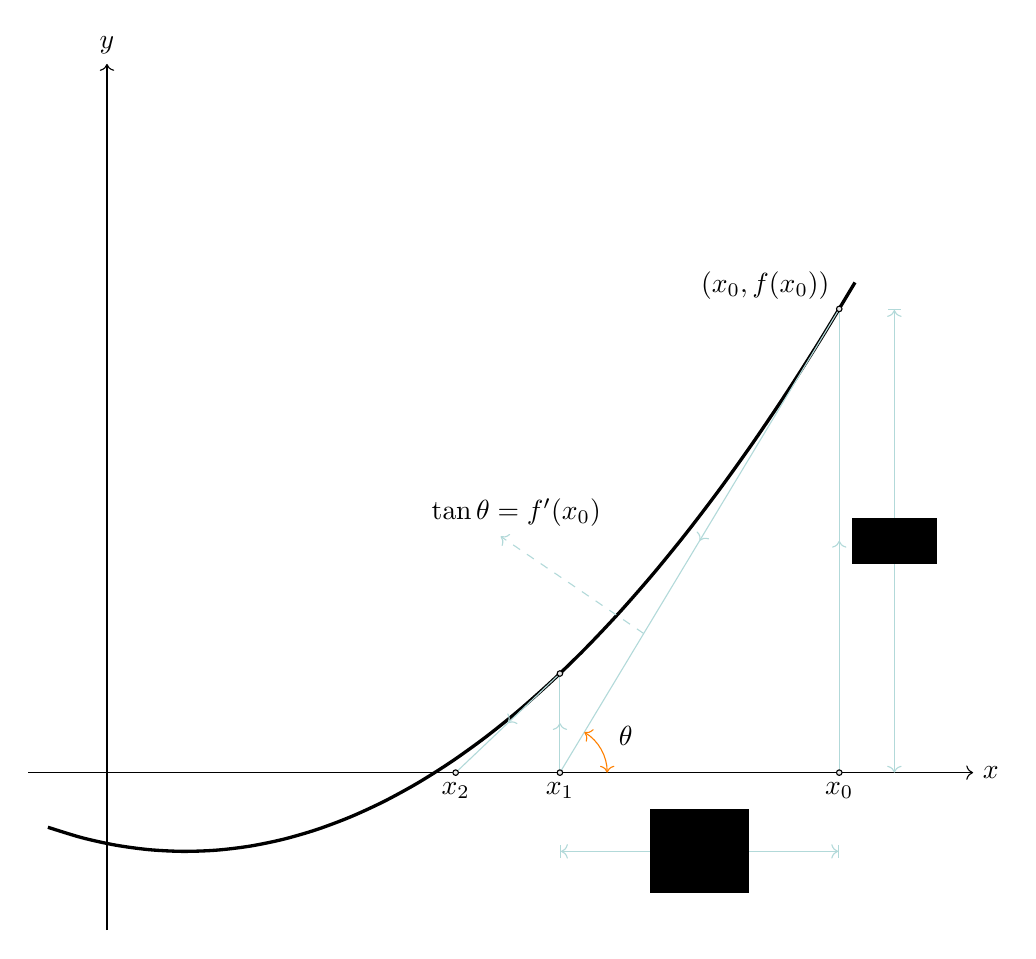
\begin{tikzpicture}[scale=1.0]
    \begin{scope}[shift={(0,0)},decoration={
        markings,
        mark=at position 0.5 with {\arrow{>}}
      }]
      \draw[->](-1,0)--(11,0)node[right]{$x$};
      \draw[->](0,-2)--(0,9)node[above]{$y$};
      \draw[very thick,domain=-.75:9.5,smooth,variable=\x]plot({\x},{.1*(\x-1)*(\x-1)-1});
      \coordinate[label=below:$x_0$] (x0) at (9.3,0);
      \coordinate[label=above left:{$\left( x_0,f(x_0)\right)$}] (f0) at (9.3,5.889);
      \coordinate[label=below:$x_1$] (x1) at (5.7524,0);
      \coordinate (f1) at (5.7524,1.2585);
      \coordinate[label=below:$x_2$] (x2) at (4.4283,0);
      \coordinate (f2) at (4.4283,0.1753);
      \draw[help lines,postaction={decorate}](x0)--(f0);
      \draw[help lines,postaction={decorate}](f0)--(x1);
      \draw[help lines,postaction={decorate}](x1)--(f1);
      \draw[help lines,postaction={decorate}](f1)--(x2);%--(f2);
      \tkzDrawPoints(x0,f0,x1,f1,x2)
      \draw[help lines,|<->|](9.3,-1)--(5.7524,-1)node[midway,fill=white,black]{$\dfrac{f(x_0)}{f'(x_0)}$};
      \draw[help lines, <->|](10,0)--(10,5.889)node[midway,fill=white,black]{$f(x_0)$};
      \draw pic["$\theta$",<->,draw=orange,angle eccentricity=1.6,angle radius=.6cm]{angle=x0--x1--f0};
      \coordinate (f) at ($.7*(x1)+.3*(f0)$);
      \coordinate[label=above:{切线斜率$\tan\theta=f'(x_0)$}] (t) at (5,3);
      \draw[dashed,->,help lines](f)--(t);
    \end{scope}
    \begin{scope}[shift={(0,0)}]
      
    \end{scope}
  \end{tikzpicture}
  \caption{牛顿切线法}
  \label{fig:numeric-newton-method}
\end{figure}

\section{二分迭代}
\label{sec:bi-section-iteration-in-numerical-analysis}

\begin{example}
  用数值方法求$x^3+x^2=1$的一个实根。
\end{example}
\begin{proof}[提示]
  实系数方程若有虚根,则都是成对出现的,从而3次方程至少有一个实根。令$f(x)=x^3+x^2-1$,则$f(1)=1>0$,$f(0)=-1<0$,由$f(x)$的连续性,其曲线在$[0,1]$内必穿过$x$轴,即在$[0,1]$必有一实根。利用二分法,可以不断缩小实根所在的区间。选择新区间的关键点在于函数值在两端点处符号要相反,即一正一负。
  \begin{table}[htbp]
    \centering
    \caption{二分法求实根}
    \label{tab:real-root-by-binary-section}
    \begin{tabular}{ccccccc}
      \hline
      迭代 & $x_1$ & $f(x_1)$ & $x_2$ & $f(x_2)$ & $\dfrac{x_1+x_2}{2}$ & $f\left(\dfrac{x_1+x_2}{2}\right)$\\\hline
      1 & 0 & $<0$ & 1 & $>0$ & 0.5  & $< 0$\\
      2 & 0.5 &  & 1 &   & 0.75 & $<0$\\
      3 & 0.75 & & 1 &   & 0.875 & $>0$\\
      4 & 0.75 & & 0.875&& 0.8125 & $ >0$\\
      5 & 0.75 & & 0.8125&& 0.78125 & $>0$\\
      6 & 0.75 & & 0.78125&& 0.765625 & $>0$\\
      7 & 0.75 & & 0.765625&& 0.7578125 & $>0$\\
      8 & 0.75 & & 0.7578125&& $\cdots$ & $\cdots$\\
      \hline
    \end{tabular}
  \end{table}
\end{proof}

\chapter{归纳}
\label{chap:induction}

\begin{definition}
  一个命题,若满足以下条件:
  \begin{enumerate}
  \item 存在非负整数$k_0$,命题在$n=k_0$时成立;
  \item 假设命题在$n\le k$时成立可以推出命题在$n=k+1$时成立。
  \end{enumerate}
  则该命题对任意整数$n\ge k_0$都成立。此证明方法称为数学归纳法。
\end{definition}

\begin{example}[求和]
  \begin{align*}
    \frac1{1\times2}+\frac1{2\times3}+\frac1{3\times4}+\cdots+\frac1{n\times (n+1)}
  \end{align*}
\end{example}

可以利用拆项,由$\dfrac1{k\times (k+1)}=\dfrac1k-\dfrac1{k+1}$,从而有
\begin{align*}
  &\frac1{1\times2}+\frac1{2\times3}+\frac1{3\times4}+\cdots+\frac1{(n-1)\times n}\\
  =&\left(\frac11-\frac13\right) + \left(\frac13-\frac14\right) + \cdots + \left(\frac1n-\frac1{n+1}\right)\\
  =&\frac11-\frac1{n+1}\\
  =&\frac{n}{n+1}
\end{align*}

若观察不到拆项的规律,可以考虑一下数学归纳法。记当$n=k$时的和为$S_k$,则
\begin{enumerate}
\item 当$n=1$时,有$S_1=\dfrac12$;
\item 当$n=2$时,有$S_2=\dfrac23$;
\item 当$n=3$时,有$S_3=\dfrac34$;
\item $\cdots$
\end{enumerate}
猜测,$\forall n$,有$S_n=\dfrac{n}{n+1}$。
\begin{proof}
  当$n=1$时,显然成立。

  设当$n\le k$时成立,考虑$n=k+1$的情况。
  \begin{align*}
    S_{k+1}&=S_k + \frac1{(k+1)\times(k+2)}\\
           &=\frac{k}{k+1}+\frac1{(k+1)\times(k+2)}\\
           &=\frac{k(k+2)+1}{(k+1)(k+2)}\\
           &=\frac{k^2+2k+1}{(k+1)(k+2)}\\
           &=\frac{k+1}{k+2}
  \end{align*}
  从而对任意整数$n\ge1$,猜测成立。
\end{proof}




\chapter{面积}
\label{chap:area}

\section{基本公式}
\label{sec:basic-area-formula}

% \begin{table}[htbp]
%   \centering
%   \renewcommand{\arraystretch}{1.2}
%   % The > directive lets you basically inject the contained code
%   % before each entry in that column.
%   % 
%   % The point of \arraybackslash is to return \\ to its original
%   % meaning because the \centering command alters this and could
%   % possibly give you a noalign error during compilation.
%   % \newcolumntype{C}{ >{\centering\arraybackslash} m{1cm} }
%   % \newcolumntype{D}{ >{\centering\arraybackslash} m{2cm} }
%   % \newcolumntype{E}{ >{\centering\arraybackslash} m{4cm} }
%   % \newcolumntype{F}{ >{\centering\arraybackslash} m{6cm} }

%   % define "struts", as suggested by Claudio Beccari in
%   % a piece in TeX and TUG News, Vol. 2, 1993.
%   % \newcommand\Tstrut{\rule{0pt}{2.6ex}}         % = `top' strut
%   % \newcommand\Bstrut{\rule[-0.9ex]{0pt}{0pt}}   % = `bottom' strut
  
%   \begin{tabular}{cccl}
%     \hline
%     序号&图形 & 示例 & 公式\\
%     \hline\\[2pt]
%     1 & 三角形 & \tikz{\draw(2,2)--(0,0)--(3,0)--(2,2)--(2,0)
%                             (1.8,0)--(1.8,.2)--(2,.2);
%                  \draw[|<->|](0,-.3)--(3,-.3)node[midway,fill=white]{$a$};
%                  \draw[|<->|](3.5, 0)--(3.5, 2)node[midway,fill=white]{$h$};
%                  } & $S=\frac12 ah$\\
%     2 & 矩阵 & \tikz{
%                \draw(0,0)rectangle(3,2);
%                \draw[|<->|](0,-.3)--(3,-.3)node[midway,fill=white]{$a$};
%                \draw[|<->|](3.5,0)--(3.5,2)node[midway,fill=white]{$b$};
%                } & $S=ab$\\
%     \hline
%   \end{tabular}
%   \caption{基本面积公式}
%   \label{tab:basic-area-formula}
% \end{table}

一些基本图形的面积公式列表如下:
\begin{center}
\begin{tikzpicture}
  \begin{scope}[shift={(0,0)}]
    \draw(2,2)--(0,0)--(3,0)--(2,2)--(2,0)
    (1.8,0)--(1.8,.2)--(2,.2);
    \draw[|<->|](0,-.3)--(3,-.3)node[midway,fill=white]{$a$};
    \draw[|<->|](3.5, 0)--(3.5, 2)node[midway,fill=white]{$h$};
    \node[right]at (4,1){$S=\dfrac12 ah$};
  \end{scope}

  \begin{scope}[shift={(8,0)}]
    \draw(0,0)rectangle(3,2);
    \draw[|<->|](0,-.3)--(3,-.3)node[midway,fill=white]{$a$};
    \draw[|<->|](3.5,0)--(3.5,2)node[midway,fill=white]{$b$};
    \node[right]at (4,1){$S=ab$};
  \end{scope}

  \begin{scope}[shift={(0,-4)}]
    \draw[|<->|](1,2.3)--(2.5,2.3)node[midway,fill=white]{$b$};
    \draw[|<->|](0,-.3)--(3,-.3)node[midway,fill=white]{$a$};
    \draw[|<->|](3.5,0)--(3.5,2)node[midway,fill=white]{$h$};
    \draw(0,0)--(3,0)--(2.5,2)--(1,2)--cycle;
    \node[right]at (4,1){$S=\dfrac12 (a+b)h$};
  \end{scope}

  \begin{scope}[shift={(8,-4)}]
    \draw(1.5,1)circle(1.5);
    \draw[->](1.5,1)--(3,1)node[midway,above]{$r$};
    \node[right]at(4,1){$S=\pi r^2$};
  \end{scope}

  \begin{scope}[shift={(0,-8)}]
    \draw(0,1)node(O){}--(3,1)node(A){} arc(0:30:3) node(B){}--cycle;
    \draw[|<->|](0,.6)--(3,.6)node[midway,below]{$r$};
    \draw pic["$\theta$",<->,draw=orange,angle eccentricity=1.6,angle radius=.6cm]{angle=A--O--B};
    \node[right]at(4,1.5){$S=\dfrac12 \theta r^2$};
  \end{scope}
\end{tikzpicture}
\end{center}

\begin{example}
  已知正方形边长,求阴影面积。

  \centering
  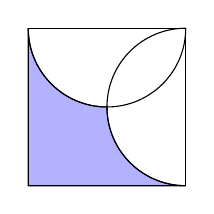
\begin{tikzpicture}[scale=2.0]
    \draw[fill=blue!30](0,0)--(1,0)arc(-90:-180:.5)arc(-90:-180:.5)--cycle;
    \draw(0,0)--(1,0)--(1,1)--(0,1)--cycle;
    \draw(1,0)arc(-90:-270:.5) (1,1)arc(0:-180:.5);
  \end{tikzpicture}
\end{example}

\hints 作辅助线,分别求各部分面积。

\begin{center}
  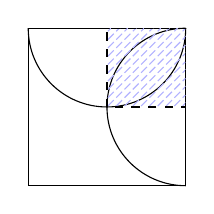
\begin{tikzpicture}[scale=2.0]
    % \draw[fill=blue!30](0,0)--(1,0)arc(-90:-180:.5)arc(-90:-180:.5)--cycle;
    \draw(0,0)--(1,0)--(1,1)--(0,1)--cycle;
    \draw(1,0)arc(-90:-270:.5) (1,1)arc(0:-180:.5);
    \draw[dashed,pattern=north east lines,pattern color=blue!30](.5,.5)rectangle(1,1);
  \end{tikzpicture}
\end{center}

\begin{example}
  求阴影面积

  \centering
  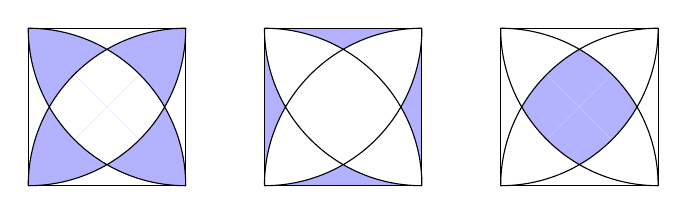
\begin{tikzpicture}[scale=1.0]
    \begin{scope}[shift={(0,0)}]
      \draw(0,0)rectangle(2,2);
      \draw[fill=blue!30,even odd rule]
           ([shift=(0:2)]0,0)arc(0:90:2)
           ([shift=(90:2)]2,0)arc(90:180:2)
           ([shift=(180:2)]2,2)arc(180:270:2)
           ([shift=(270:2)]0,2)arc(270:360:2);
    \end{scope}

    \begin{scope}[shift={(3,0)}]
      \fill[color=blue!30] (0,0)--(2,0) arc(-90:-120:2) arc(-60:-90:2);
      \fill[color=blue!30] (2,0)--(2,2) arc(0:-30:2) arc(30:0:2);
      \fill[color=blue!30] (2,2)--(0,2) arc(90:60:2) arc(120:90:2);
      \fill[color=blue!30] (0,2)--(0,0) arc(180:150:2) arc(210:180:2);
      \draw(0,0)rectangle(2,2);
      \draw([shift=(0:2)]0,0)arc(0:90:2)
           ([shift=(90:2)]2,0)arc(90:180:2)
           ([shift=(180:2)]2,2)arc(180:270:2)
           ([shift=(270:2)]0,2)arc(270:360:2);
    \end{scope}

    \begin{scope}[shift={(6,0)}]
      \fill[color=blue!30]
           ([shift=(0:2)]0,0)arc(0:90:2)
           ([shift=(90:2)]2,0)arc(90:180:2)
           ([shift=(180:2)]2,2)arc(180:270:2)
           ([shift=(270:2)]0,2)arc(270:360:2);
      \fill[color=white,even odd rule]
           ([shift=(0:2)]0,0)arc(0:90:2)
           ([shift=(90:2)]2,0)arc(90:180:2)
           ([shift=(180:2)]2,2)arc(180:270:2)
           ([shift=(270:2)]0,2)arc(270:360:2);
      \draw(0,0)rectangle(2,2);
      \draw([shift=(0:2)]0,0)arc(0:90:2)
           ([shift=(90:2)]2,0)arc(90:180:2)
           ([shift=(180:2)]2,2)arc(180:270:2)
           ([shift=(270:2)]0,2)arc(270:360:2);
    \end{scope}
  \end{tikzpicture}
\end{example}
\begin{proof}[解]
  交点将圆弧平均分成三段,每段对应于$30^\circ$的圆弧。\hints 图中三角形是等边三角形。

  \begin{center}
  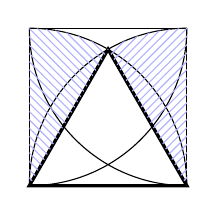
\begin{tikzpicture}[scale=1.0]
    \draw(0,0)rectangle(2,2);
    \draw([shift=(0:2)]0,0)arc(0:90:2)
         ([shift=(90:2)]2,0)arc(90:180:2)
         ([shift=(180:2)]2,2)arc(180:270:2)
         ([shift=(270:2)]0,2)arc(270:360:2);
    \coordinate (A) at (60:2);
    \draw[very thick](0,0)--(2,0)--(A)--cycle;
    \fill[pattern=north west lines,pattern color=blue!30](0,0)--(A)arc(60:90:2)--cycle;
    \fill[pattern=north east lines,pattern color=blue!30](2,0)--(2,2)arc(90:120:2)--cycle;
  \end{tikzpicture}
  \end{center}

  可按图中分割方式求解题目第二个图中阴影面积。
\end{proof}

\begin{example}
  由两个圆弧组成的图形称为半月形(lune)。求图中阴影部分半月形的面积。

  \centering
  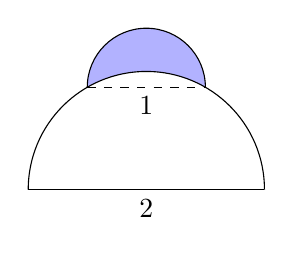
\begin{tikzpicture}[scale=1.5]
    \coordinate (O) at (0,0);
    \coordinate (A) at (120:1); 
    \coordinate (B) at (60:1);
    \coordinate (C) at ($.5*(A) + .5*(B)$);
    \draw[fill=blue!30](B)arc(0:180:.5);
    \draw[fill=white](1,0)arc(0:180:1);
    \draw[dashed](A)--(B) node[midway,below]{$1$};
    \draw(-1,0)--(1,0) node[midway, below]{$2$};;
  \end{tikzpicture}
\end{example}
\begin{proof}[提示]
  可转换为求弓形面积。

  \begin{center}
    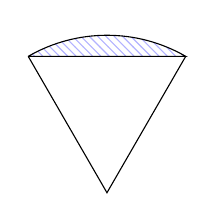
\begin{tikzpicture}[scale=2.0]
      \coordinate (O) at (0,0);
      \coordinate (A) at (120:1);
      \coordinate (B) at (60:1);
      \draw[pattern=north west lines, pattern color=blue!30](A)--(B) arc(60:120:1);
      \draw(A)--(O)--(B);
    \end{tikzpicture}
  \end{center}

  弓形面积可由上图中分割方式求出,即扇形面积减三角形面积。
\end{proof}

\begin{example}
  图中四边形为单位正方形,求阴影面积。

  \centering
  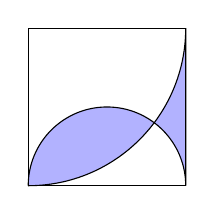
\begin{tikzpicture}[scale=1.0]
    \draw[fill=blue!30,even odd rule](0,0)arc(-90:0:2)--(2,0)arc(0:180:1);
    \draw(2,0)--(0,0)--(0,2)--(2,2);
  \end{tikzpicture}
\end{example}
\begin{proof}[解]
  除了积分,暂时未发现有其它好方法。
  \begin{align*}
    S&=\int_{x=0}^1 \left| \sqrt{0.5^2 - (x-0.5)^2} - \left(1-\sqrt{1-x^2}\right)\right| \dx\qedhere
  \end{align*}
\end{proof}

\begin{example}
  已知三角形面积为$1$,求阴影面积。其中第一个图的线段长度的比例如图所示。后两图,若其中线段长度的比例都已知,则阴影面积又该如何求解?

  \centering
  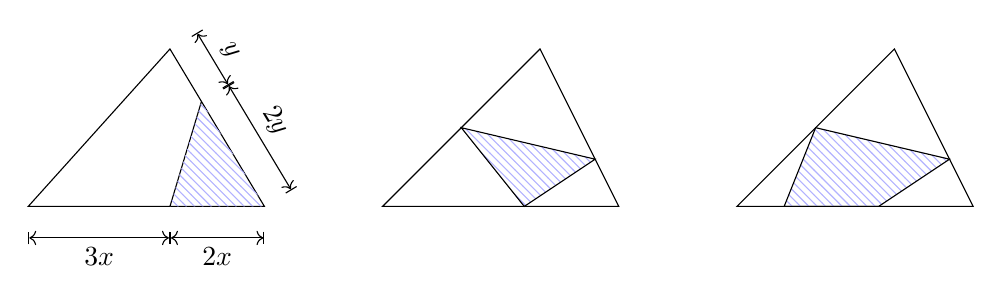
\begin{tikzpicture}[scale=1.0]
    \begin{scope}[shift={(0,0)}]
      \coordinate (A) at (1.8,2);
      \coordinate (B) at (0,0);
      \coordinate (C) at (3,0);
      \coordinate (D) at ($.6*(C)$);
      \coordinate (E) at ($2/3*(A)+1/3*(C)$);
      \draw(A)--(B)--(C)--cycle (D)--(E);
      \fill[pattern=north west lines,pattern color=blue!30](C)--(D)--(E)--cycle;

      \coordinate (B') at ($(0,-.4) + (B)$);
      \coordinate (C') at ($(0,-.4) + (C)$);
      \coordinate (D') at ($(0,-.4) + (D)$);
      \draw[|<->|](B')--(D') node[midway,below]{$3x$};
      \draw[|<->|](D')--(C') node[midway,below]{$2x$};

      \coordinate (P)  at ($({.4*2/sqrt(5.44)}, {.4*1.2/sqrt(5.44)})$);
      \coordinate (C') at ($(P) + (C)$);
      \coordinate (E') at ($(P) + (E)$);
      \coordinate (A') at ($(P) + (A)$);
      \draw[|<->|](C')--(E') node[pos=.75,above right,sloped]{$2y$};
      \draw[|<->|](E')--(A') node[pos=.75,above right,sloped]{$y$};
    \end{scope}

    \begin{scope}[shift={(4.5,0)}]
      \coordinate (B) at (0,0);
      \coordinate (C) at (3,0);
      \coordinate (A) at (2,2);
      \coordinate (D) at ($.4*(B) + .6*(C)$);
      \coordinate (E) at ($.3*(A) + .7*(C)$);
      \coordinate (F) at ($.5*(A) + .5*(B)$);
      \draw(A)--(B)--(C)--cycle;
      \draw[pattern=north west lines,pattern color=blue!30](D)--(E)--(F)--cycle;
    \end{scope}

    \begin{scope}[shift={(9,0)}]
      \coordinate (B) at (0,0);
      \coordinate (C) at (3,0);
      \coordinate (A) at (2,2);
      \coordinate (D) at ($.4*(B) + .6*(C)$);
      \coordinate (E) at ($.3*(A) + .7*(C)$);
      \coordinate (F) at ($.5*(A) + .5*(B)$);
      \coordinate (G) at ($.8*(B) + .2*(C)$);
      \draw(A)--(B)--(C)--cycle;
      \draw[pattern=north west lines,pattern color=blue!30](D)--(E)--(F)--(G)--cycle;
    \end{scope}

  \end{tikzpicture}
\end{example}
\begin{proof}[解]\mbox{}\\
  \begin{center}
    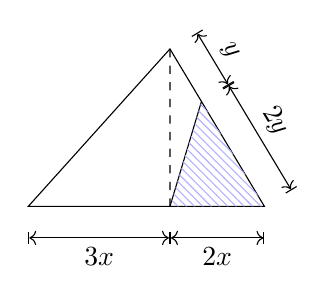
\begin{tikzpicture}[scale=1.0]
    \begin{scope}[shift={(0,0)}]
      \coordinate (A) at (1.8,2);
      \coordinate (B) at (0,0);
      \coordinate (C) at (3,0);
      \coordinate (D) at ($.6*(C)$);
      \coordinate (E) at ($2/3*(A)+1/3*(C)$);
      \draw(A)--(B)--(C)--cycle (D)--(E);
      \fill[pattern=north west lines,pattern color=blue!30](C)--(D)--(E)--cycle;

      \coordinate (B') at ($(0,-.4) + (B)$);
      \coordinate (C') at ($(0,-.4) + (C)$);
      \coordinate (D') at ($(0,-.4) + (D)$);
      \draw[|<->|](B')--(D') node[midway,below]{$3x$};
      \draw[|<->|](D')--(C') node[midway,below]{$2x$};

      \coordinate (P)  at ($({.4*2/sqrt(5.44)}, {.4*1.2/sqrt(5.44)})$);
      \coordinate (C') at ($(P) + (C)$);
      \coordinate (E') at ($(P) + (E)$);
      \coordinate (A') at ($(P) + (A)$);
      \draw[|<->|](C')--(E') node[pos=.75,above right,sloped]{$2y$};
      \draw[|<->|](E')--(A') node[pos=.75,above right,sloped]{$y$};

      \draw[dashed](A)--(D);
    \end{scope}
  \end{tikzpicture}
\end{center}

  作辅助线,可以容易看出各个三角形之间的面积关系。
\end{proof}

\section{面积法}
\label{sec:area-method}

有时解决问题可以升维或降维。比如在某些情况下求解线段问题时,可以升维成面积问题。反之,有时求解体积问题时可以降维成线段问题。

\begin{example}
  如图,$D$和$E$是$\triangle ABC$两边上一点,$O$是$AE$与$CD$的交点。若$\dfrac{CE}{BE}=\dfrac{u}{v}$,$\dfrac{AD}{BD}=\dfrac{x}{y}$,求$\dfrac{CO}{DO}$。
  \begin{center}
    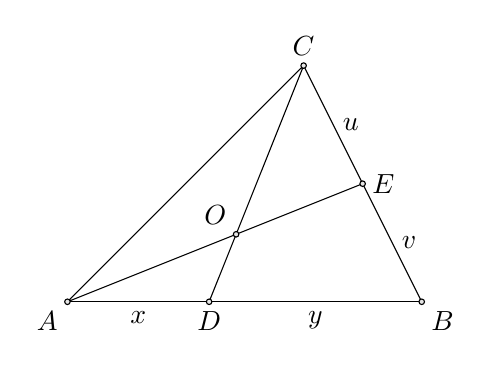
\begin{tikzpicture}[scale=1.5]
      \coordinate[label=below left:$A$](A) at (0,0);
      \coordinate[label=below right:$B$](B) at (3,0);
      \coordinate[label=above:$C$](C) at (2,2);
      \coordinate[label=below:$D$](D) at ($.6*(A)+.4*(B)$);
      \coordinate[label=right:$E$](E) at ($.5*(B)+.5*(C)$);
      \coordinate[label=above left:$O$](O) at ($2/7*(C)+5/7*(D)$);
      \draw(A)--(D) node[midway,below]{$x$};
      \draw(D)--(B) node[midway,below]{$y$};
      \draw(B)--(E) node[midway,right]{$v$};
      \draw(E)--(C) node[midway,right]{$u$};
      \draw(C)--(A)--(O)--(E) (C)--(D);
      \tkzDrawPoints(A,B,C,D,E,O)
    \end{tikzpicture}
  \end{center}
\end{example}
\begin{proof}[提示]利用面积法。如图,设$\triangle AOD$与$\triangle COE$的面积分别为$M$和$N$。
  \begin{center}
    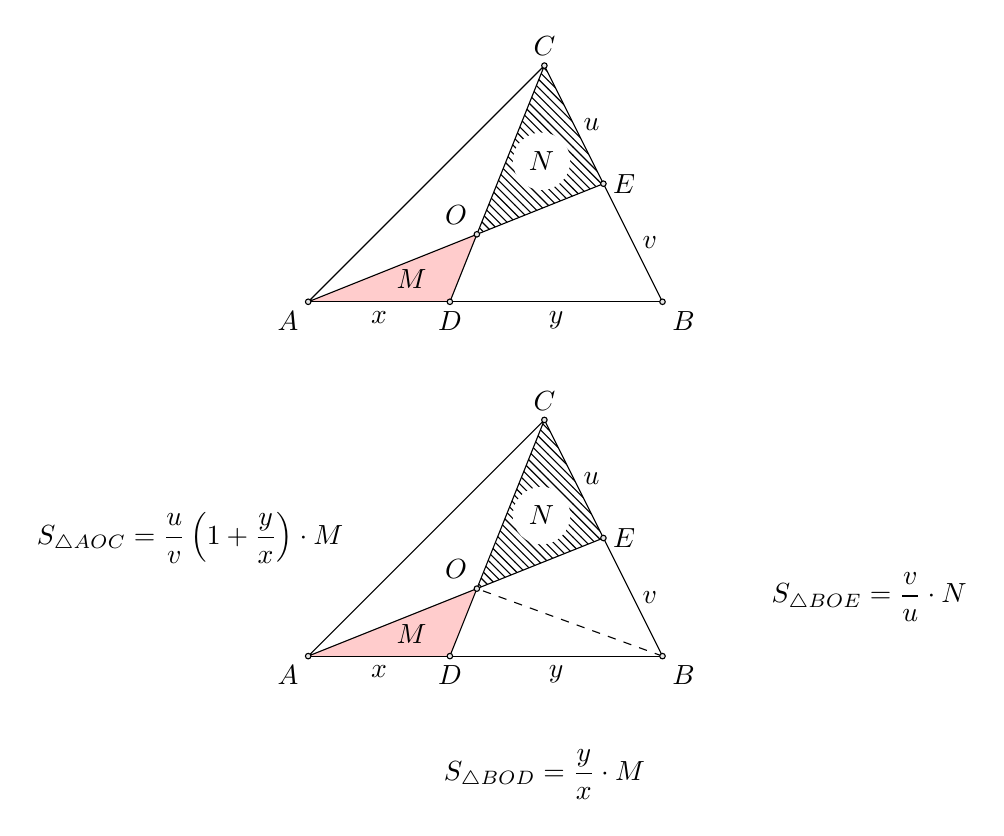
\begin{tikzpicture}[scale=1.5]
      \begin{scope}
        \coordinate[label=below left:$A$](A) at (0,0);
        \coordinate[label=below right:$B$](B) at (3,0);
        \coordinate[label=above:$C$](C) at (2,2);
        \coordinate[label=below:$D$](D) at ($.6*(A)+.4*(B)$);
        \coordinate[label=right:$E$](E) at ($.5*(B)+.5*(C)$);
        \coordinate[label=above left:$O$](O) at ($2/7*(C)+5/7*(D)$);
        \fill[color=red!20](A)--(D)--(O)--cycle;
        \fill[pattern=north west lines](C)--(E)--(O)--cycle;
        \draw(A)--(D) node[midway,below]{$x$};
        \draw(D)--(B) node[midway,below]{$y$};
        \draw(B)--(E) node[midway,right]{$v$};
        \draw(E)--(C) node[midway,right]{$u$};
        \draw(C)--(A)--(O)--(E) (C)--(D);
        \tkzDrawPoints(A,B,C,D,E,O)
        \node at ($1/3*(A)+1/3*(D)+1/3*(O)$) {$M$};
        \node[fill=white,circle] at ($1/3*(C)+1/3*(E)+1/3*(O)$) {$N$};
      \end{scope}
      \begin{scope}[shift={(0,-3)}]
        \coordinate[label=below left:$A$](A) at (0,0);
        \coordinate[label=below right:$B$](B) at (3,0);
        \coordinate[label=above:$C$](C) at (2,2);
        \coordinate[label=below:$D$](D) at ($.6*(A)+.4*(B)$);
        \coordinate[label=right:$E$](E) at ($.5*(B)+.5*(C)$);
        \coordinate[label=above left:$O$](O) at ($2/7*(C)+5/7*(D)$);
        \fill[color=red!20](A)--(D)--(O)--cycle;
        \fill[pattern=north west lines](C)--(E)--(O)--cycle;
        \draw(A)--(D) node[midway,below]{$x$};
        \draw(D)--(B) node[midway,below]{$y$};
        \draw(B)--(E) node[midway,right]{$v$};
        \draw(E)--(C) node[midway,right]{$u$};
        \draw(C)--(A)--(O)--(E) (C)--(D);
        \draw[dashed](B)--(O);
        \tkzDrawPoints(A,B,C,D,E,O)
        \node at ($1/3*(A)+1/3*(D)+1/3*(O)$) {$M$};
        \node[fill=white,circle] at ($1/3*(C)+1/3*(E)+1/3*(O)$) {$N$};
        \node(SBOE) at ($.5*(B)+.5*(E)+(2,0)$) {$S_{\triangle BOE} = \dfrac{v}{u}\cdot N$};
        \node(SBOD) at ($(B)+(-1,-1)$) {$S_{\triangle BOD}=\dfrac{y}{x}\cdot M$};
        \node(SAOC) at ($.5*(A)+.5*(C)+(-2,0)$) {$S_{\triangle AOC}=\dfrac{u}{v}\left(1+\dfrac{y}{x}\right)\cdot M$};
    \end{scope}
    \end{tikzpicture}
  \end{center}
  连接$BO$,可分别求得各部分的面积,即
  \begin{align*}
    &S_{\triangle BOD} = \frac{y}{x}\cdot M,\quad\quad
    S_{\triangle BOE} = \frac{v}{u}\cdot N\\
    \implies& S_{\triangle ABE} = \left(1 + \frac{y}{x}\right)\cdot M + \frac{v}{u}\cdot N \\
    \implies& S_{\triangle ACE} = \frac{u}{v}\cdot S_{\triangle ABE} =
              \frac{u}{v}\left(1+\frac{y}{x}\right)\cdot M + N\\
    \implies& S_{\triangle AOC} = \frac{u}{v}\left(1+\frac{y}{x}\right)\cdot M
  \end{align*}
  由此可得
  \begin{align*}
    \frac{CO}{DO}= & \frac{S_{\triangle AOC}}{S_{\triangle AOD}}= \frac{u}{v}\left(1+\frac{y}{x}\right)
  \end{align*}

  这里还可以得到关于$M$与$N$之间关系的结论。由类似的方法得到$S_{\triangle AOC}$关于$N$的表达式为
  \begin{align*}
    & S_{\triangle AOC} = \frac{x}{y}\left(1+\frac{v}{u}\right)\cdot N\\
    \implies & \frac{u}{v}\left(1+\frac{y}{x}\right)\cdot M = \frac{x}{y}\left(1+\frac{v}{u}\right)\cdot N\qedhere
  \end{align*}
\end{proof}

\begin{example}[正八边形]
  若正八边形最长的对角线为$a$,最短的对角线为$b$,则正八边形的面积是$ab$。
  \begin{center}
    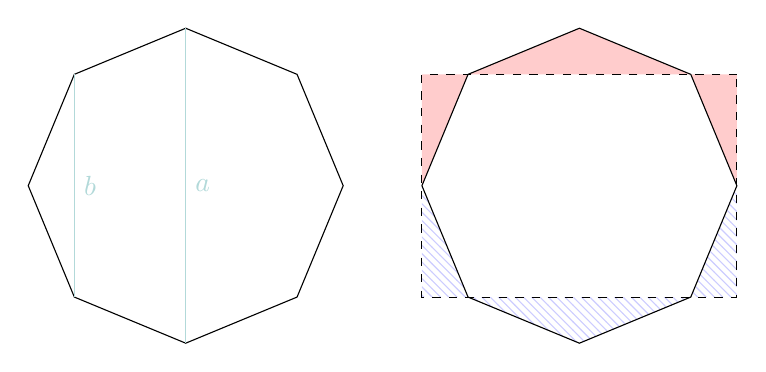
\begin{tikzpicture}[scale=1.0]
      \begin{scope}
        \foreach \i in{0,1,2,3,4,5,6,7}{%
          \coordinate(N\i) at (360/8*\i:2);
        }
        \draw(N0)--(N1)--(N2)--(N3)--(N4)--(N5)--(N6)--(N7)--cycle;
        \draw[help lines](N2)--(N6)node[midway,right]{$a$};
        \draw[help lines](N3)--(N5)node[midway,right]{$b$};
      \end{scope}
      \begin{scope}[shift={(5,0)}]
        \foreach \i in{0,1,2,3,4,5,6,7}{%
          \coordinate(N\i) at (360/8*\i:2);
        }

        \coordinate(A) at ($(N1)!(N0)!(N3)$);
        \coordinate(B) at ($(N1)!(N4)!(N3)$);
        \coordinate(C) at ($(N5)!(N4)!(N7)$);
        \coordinate(D) at ($(N5)!(N0)!(N7)$);
        % \coordinate(E) at ($(N1)!(N2)!(N3)$);
        % \coordinate(F) at ($(N5)!(N6)!(N7)$);
        \fill[red!20](N1)--(N2)--(N3);
        \fill[red!20](N0)--(A)--(N1)--cycle (N3)--(B)--(N4)--cycle;
        \fill[pattern=north west lines,pattern color=blue!20](N5)--(N6)--(N7)--cycle;
        \fill[pattern=north west lines,pattern color=blue!20](N4)--(C)--(N5)--cycle (N7)--(D)--(N0)--cycle;

        \draw[dashed](A)--(B)--(C)--(D)--cycle;
        \draw(N0)--(N1)--(N2)--(N3)--(N4)--(N5)--(N6)--(N7)--cycle;
      \end{scope}
    \end{tikzpicture}
  \end{center}
\end{example}
\begin{proof}[提示]
  由上图,将正八边形切割后可重新拼装成一个$a\times b$的长方形。
\end{proof}

\begin{example}
  如图,$E$是正方形$ABCD$的$AB$边的中点,且阴影面积为$45$,求正方形的面积。
  \begin{center}
    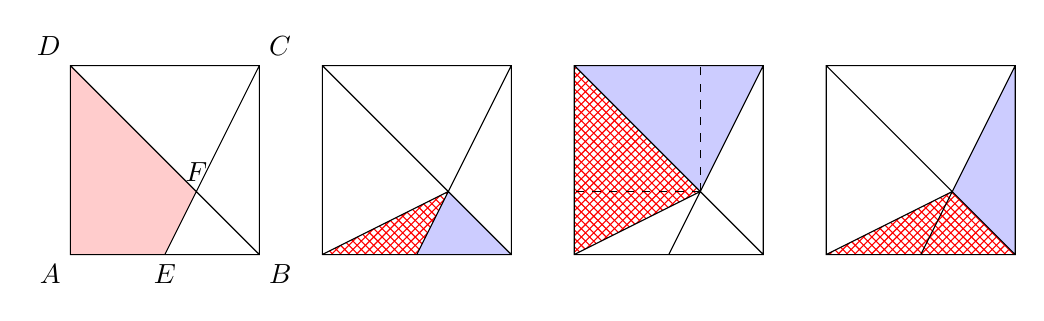
\begin{tikzpicture}[scale=.8]
      \coordinate[label=below left:$A$](A)at(0,0);
      \coordinate[label=below right:$B$](B)at(3,0);
      \coordinate[label=above right:$C$](C)at(3,3);
      \coordinate[label=above left:$D$](D)at(0,3);
      \coordinate[label=below:$E$](E)at($.5*(A)+.5*(B)$);
      \tkzInterLL(B,D)(E,C)\tkzGetPoint{F}
      \fill[color=red!20](A)--(E)--(F)--(D)--cycle;
      \draw(A)--(B)--(C)--(D)--cycle (E)--(C) (D)--(B);
      \tkzLabelPoints[above](F)
      \begin{scope}[shift={(4,0)}]
        \coordinate(A)at(0,0);
        \coordinate(B)at(3,0);
        \coordinate(C)at(3,3);
        \coordinate(D)at(0,3);
        \coordinate(E)at($.5*(A)+.5*(B)$);
        \tkzInterLL(B,D)(E,C)\tkzGetPoint{F}
        % \fill[color=red!20](A)--(E)--(F)--(D)--cycle;
        \fill[pattern=crosshatch,pattern color=red](A)--(F)--(E)--cycle;
        \fill[color=blue!20](F)--(E)--(B)--cycle;
        \draw(A)--(B)--(C)--(D)--cycle (E)--(C) (D)--(B) (A)--(F);
      \end{scope}
      \begin{scope}[shift={(8,0)}]
        \coordinate(A)at(0,0);
        \coordinate(B)at(3,0);
        \coordinate(C)at(3,3);
        \coordinate(D)at(0,3);
        \coordinate(E)at($.5*(A)+.5*(B)$);
        \tkzInterLL(B,D)(E,C)\tkzGetPoint{F}
        % \fill[color=red!20](A)--(E)--(F)--(D)--cycle;
        \fill[pattern=crosshatch,pattern color=red](A)--(F)--(D)--cycle;
        \fill[color=blue!20](C)--(F)--(D)--cycle;
        \draw(A)--(B)--(C)--(D)--cycle (E)--(C) (D)--(B) (A)--(F);
        \draw[dashed](F)--(F |- D) (F)--(F -| D);
      \end{scope}
      \begin{scope}[shift={(12,0)}]
        \coordinate(A)at(0,0);
        \coordinate(B)at(3,0);
        \coordinate(C)at(3,3);
        \coordinate(D)at(0,3);
        \coordinate(E)at($.5*(A)+.5*(B)$);
        \tkzInterLL(B,D)(E,C)\tkzGetPoint{F}
        % \fill[color=red!20](A)--(E)--(F)--(D)--cycle;
        \fill[pattern=crosshatch,pattern color=red](A)--(F)--(B)--cycle;
        \fill[color=blue!20](C)--(F)--(B)--cycle;
        \draw(A)--(B)--(C)--(D)--cycle (E)--(C) (D)--(B) (A)--(F);
        % \draw[dashed](F)--(F |- D) (F)--(F -| D);
      \end{scope}
    \end{tikzpicture}
  \end{center}
\end{example}
\begin{proof}[提示]
  由后面几个图形,由两部分阴影面积相等可以知道只要得出$\triangle DFC$和$\triangle BFC$的面积比,即只要得出$DF:BF$就可以得到图中各种三角形的面积关系,从而由$S_{AEFD}=45$可以求出各个面积。

  \begin{center}
    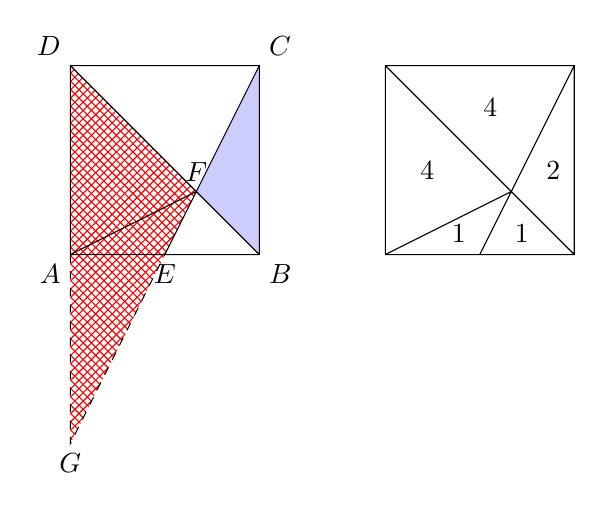
\begin{tikzpicture}[scale=.8]
      \begin{scope}[shift={(0,0)}]
        \coordinate[label=below left:$A$](A)at(0,0);
        \coordinate[label=below right:$B$](B)at(3,0);
        \coordinate[label=above right:$C$](C)at(3,3);
        \coordinate[label=above left:$D$](D)at(0,3);
        \coordinate[label=below:$E$](E)at($.5*(A)+.5*(B)$);
        \tkzInterLL(B,D)(E,C)\tkzGetPoint{F}
        \coordinate[label=below:$G$](G)at(0,-3);
        % \fill[color=red!20](A)--(E)--(F)--(D)--cycle;
        \fill[pattern=crosshatch,pattern color=red](G)--(F)--(D)--cycle;
        \fill[color=blue!20](C)--(F)--(B)--cycle;
        \draw(A)--(B)--(C)--(D)--cycle (E)--(C) (D)--(B) (A)--(F);
        \draw[dashed](A)--(G)--(E);
        % \draw[dashed](F)--(F |- D) (F)--(F -| D);
        \tkzLabelPoints[above](F)
      \end{scope}      
      \begin{scope}[shift={(5,0)}]
        \coordinate(A)at(0,0);
        \coordinate(B)at(3,0);
        \coordinate(C)at(3,3);
        \coordinate(D)at(0,3);
        \coordinate(E)at($.5*(A)+.5*(B)$);
        \tkzInterLL(B,D)(E,C)\tkzGetPoint{F}
        \draw(A)--(B)--(C)--(D)--cycle (E)--(C) (D)--(B) (A)--(F);
        \node at($1/3*(A)+1/3*(E)+1/3*(F)$){1};
        \node at($1/3*(B)+1/3*(E)+1/3*(F)$){1};
        \node at($1/3*(B)+1/3*(C)+1/3*(F)$){2};
        \node at($1/3*(A)+1/3*(F)+1/3*(D)$){4};
        \node at($1/3*(C)+1/3*(F)+1/3*(D)$){4};
      \end{scope}
    \end{tikzpicture}
  \end{center}
  如上图,延长$CE$与$DA$相交于$G$,可知$AG=BC$,从而$DF:FB=DG:BC=2$。由此可得上面第二图中各面积关系比。
\end{proof}

\begin{example}
  由上面分析,容易得到正方形一个顶点与两条不相邻边的中点的连线将一条对角线三等分。
  \begin{center}
    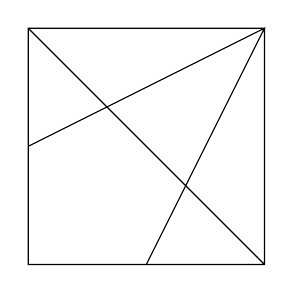
\begin{tikzpicture}
      \begin{scope}
        \coordinate(A)at(0,0);
        \coordinate(B)at(3,0);
        \coordinate(C)at(3,3);
        \coordinate(D)at(0,3);
        \coordinate(E)at($.5*(A)+.5*(B)$);
        \coordinate(F)at($.5*(A)+.5*(D)$);
        \draw(A)--(B)--(C)--(D)--cycle (E)--(C)--(F) (D)--(B);
      \end{scope}      
    \end{tikzpicture}
  \end{center}
\end{example}

\chapter{二次方程}
\label{chap:quadratic-equation}

\begin{definition}[一元二次方程]
  对常数$a,b,c$及未知数$x$,以下方程称为一元二次方程
  \begin{align*}
    ax^2+bx+c=0
  \end{align*}
\end{definition}

若$a=0$,则方程退化为一元一次方程。当$a\ne0$时用配方法消去$x$的一次项可求解:
\begin{align*}
  &ax^2+bx+c=0\\
  \implies& a\cdot\left(x^2+\frac ba x + \frac{b^2}{4a^2}\right) - a\cdot\frac{b^2}{4a^2} + c = 0\\
  \implies& a\cdot\left(x+\frac{b}{2a}\right)^2=\frac{b^2-4ac}{4a}\\
  \implies& x+\frac{b}{2a} =\pm\sqrt{\frac{b^2-4ac}{4a^2}}\\
  \implies& x=-\frac{b}{2a}\pm\frac{\sqrt{b^2-4ac}}{2|a|}\\
  \implies& x=-\frac{b}{2a}\pm\frac{\sqrt{b^2-4ac}}{2a}\\
  \implies& x=\frac{-b\pm\sqrt{b^2-4ac}}{2a}
\end{align*}
即一元二次方程有实数根,当且仅当$b^2\ge4ac$,当月$b^2=4ac$时有重根。


\chapter{函数}
\label{chap:function}

\begin{definition}[对合,Involution]
  一个函数若存在反函数且其反函数为其本身,则称此函数为对合或对合函数。
\end{definition}

\begin{example}
  以下三个都是对合函数的例子:
  \begin{align*}
    f(x)=x,\quad g(x)=\frac1x,\quad h(x)=\frac{x}{x-1}
  \end{align*}
\end{example}

\begin{example}
  存在无限个对合函数。
\end{example}
\begin{proof}
  显然,一个函数是对合函数$\iff$其在笛卡尔坐标下的曲线关于直线$y=x$对称,这样的曲线是可以无限地构造出来。比如任意非零实数$a$,$f(x)=\frac{a}{x}$都是对合函数。或者,利用下面的定理构造。
\end{proof}

\begin{theorem}
  若$f$是对合函数,$g$有反函数$\bar g$,则$h\equiv g\circ f\circ\bar g$是对合函数。
\end{theorem}
\begin{proof}
  任意定义域内$x$,有
  \begin{align*}
    h(x)&= g(f(\bar g(x)))\\
    h(h(x))&=g(f(\underline{\bar g( g}(f(\bar g(x))) ))) = g(\underline{f(f}(\bar g(x)))) = g(\bar g(x)) = x \qedhere
  \end{align*}
\end{proof}

\chapter{对称性}
\label{chap:symetric}

\begin{example}
  求解方程 $x^4+x^3+x^2+x+1=0$。
\end{example}
\begin{proof}[解]
  利用系数的对称性及$x\ne 0$,两边除以$x^2$,有
  \begin{align*}
    &x^2+x+1+\frac1x+\frac1{x^2}=0\\
    \implies& \left(x^2+\frac1{x^2}\right) + \left(x+\frac1x\right) + 1 = 0
  \end{align*}
  分组后令$u=x+\dfrac1x$,则有$u^2=x^2+\dfrac1{x^2}+2$,从而原方程变换为
  \begin{align*}
    u^2 + u - 1 = 0
  \end{align*}
  剩余略。
\end{proof}


\chapter{极端原理}
\label{chap:extreme}



\chapter{无穷级数}
\label{chap:inifinite-series}

\begin{example}[等比数列]
  求无穷等比数列的和,其中比例系数$q<1$:
  \begin{align*}
    S=a + aq + aq^2 + aq^3 + \cdots
  \end{align*}
\end{example}
\begin{proof}[解]
  两边同乘以$q$,有
  \begin{eqnarray*}
            & qS=& aq + aq^2 + aq^3 + aq^4 + \cdots\\
    \implies& qS=& S - a\\
    \implies&  S=& \frac{a}{1-q}
  \end{eqnarray*}
  关于无穷级数的一个技巧在于乘以其个数后找到与原数的关系。
\end{proof}

\begin{example}[$\zeta$函数]
  $\zeta$函数是按以下无穷级数定义的函数
  \begin{align}
    \zeta(x)\equiv \frac1{1^x} + \frac1{2^x} + \frac1{3^x} + \cdots
  \end{align}
  当$x=1$时,$\zeta(1)$就是调和函数。证明当$x\ge2$时,$\zeta$函数是收敛的。
\end{example}
\begin{proof}
  显然$\zeta(x)$在$x>1$时是严格单调递减正函数,从而只需考虑$\zeta(2)$的收敛性。由
  \begin{align*}
    \frac1{k^2} \le \frac1{k(k-1)},\quad\forall k>1
  \end{align*}
  从而有$\zeta(2)$的前$n$项和为
  \begin{align*}
    \zeta(2)_n&=\frac1{1^2} + \frac1{2^2} + \frac1{3^2} + \cdots + \frac1{n^2}\\
            &\le \frac1{1^2} + \frac1{2\times(2-1)} + \frac1{3\times(3-1)} +\frac1{4\times(4-1)}+ \cdots + \frac1{n\times(n-1)}\\
            &= 1 + \left(1 - \frac12\right) + \left(\frac12 - \frac13\right) + \cdots + \left(\frac1{n-1}-\frac1n\right)\\
            &= 2 - \frac1n
  \end{align*}
  令$n\to+\infty$,有$\zeta(2)\le2$。从而$\zeta(2)$有上界,收敛。
\end{proof}

\begin{example}
  求下列级数的和:
  \begin{align*}
    q + 2q^2 + 3q^3 + 4q^4 + \cdots + nq^n
  \end{align*}
\end{example}
\begin{proof}[提示]
  记其和为$S_n$,则
  \begin{align*}
    qS_n = q^2 + 2q^3 + 3q^4 + 4q^5 + \cdots + nq^{n+1}
  \end{align*}
  与原式相减,则有
  \begin{align*}
    S_n - qS_n = \underline{q + q^2 + q^3 + \cdots + q^n} - nq^{n+1}
  \end{align*}
  去掉首尾两项(下划线部分)后是等比级数,应用等比数列求和公式并化简可得。
\end{proof}

\begin{example}
  求和
  \begin{align*}
    \dfrac1{1\times2\times3} + \dfrac1{2\times3\times4} + \dfrac1{3\times4\times5} + \cdots + \dfrac1{n\times(n+1)\times(n+2)}
  \end{align*}
\end{example}
\begin{proof}[提示]
  利用下式拆项
  \begin{align*}
    \frac1{n(n+1)(n+2)} = \frac12 \left(\frac1{n(n+1)} - \frac1{(n+1)(n+2)}\right)&\qedhere
  \end{align*}
\end{proof}

\begin{example}[推广]
  是否有简单方法对下式求和
  \begin{align*}
    S_{n,k}=\sum_{i=1}^{n} \frac1{\prod_{j=i}^{i+k-1} j}
  \end{align*}
  如
  \begin{align*}
    S_{n,4} = \sum_{i=1}^{n}\frac1{i(i+1)(i+2)(i+3)}
  \end{align*}
\end{example}

\begin{example}
  对下式求和:
  \begin{align*}
    1\times2\times3 + 2\times3\times4 + 3\times4\times5 + \cdots + n(n+1)(n+2)
  \end{align*}
  并推广。
\end{example}

\begin{example}
  计算可知$\left\lfloor\sqrt{44}\right\rfloor=6$,$\left\lfloor\sqrt{4444}\right\rfloor=66$,其中$\left\lfloor x\right\rfloor$是指对$x$向下取整。请推广。
\end{example}
\begin{proof}[解]
  记
  \begin{align*}
    S_1&=44\\
    S_2&=4444\phantom{44}=100S_1+44\\
    S_3&=444444=100S_2+44\\
    \multicolumn{2}{c}{$\cdots$}\\
    S_n&=\phantom{444444=}100S_{n-1}+44
  \end{align*}
  其中$6<\sqrt{S_1}<7$。引用另一个序列$b_n$如下
  \begin{align*}
    b_1&=6\\
    b_2&=66\phantom{6}=10b_1 + 6\\
    b_3&=666          =10b_2 + 6\\
       &\cdots\\
    b_n&=\phantom{666=}10b_{n-1} + 6
  \end{align*}
  用数学归纳法。假设对任意$n\le k$,有
  \begin{align*}
    b_n<\sqrt{S_n}<b_n+1,\quad\text{即}\quad b_n^2 < S_n < (b_n+1)^2
  \end{align*}
  则对$n=k+1$,希望有
  \begin{align*}
    b_{k+1}^2 < S_{k+1} < (b_{k+1}+1)^2
  \end{align*}
  但上面的假设实在是太粗糙了,在后面确定$S_{k+1}$的上下界时无法得到需要的结果。针对上式,先考虑左边,有
  \begin{align*}
    b_{k+1}^2 < S_{k+1} \iff & (10b_k + 6)^2 < 100S_k + 44
                        \iff & (b_k + 0.6) ^2 < S_k + 0.44
  \end{align*}
  再考虑右边,有
  \begin{align*}
    S_{k+1} < (b_{k+1}+1)^2 \iff & 100S_k+44 < \left((10b_k+6)+1\right)^2 \iff S_k + 0.44 < (b_k+0.7)^2
  \end{align*}
  由此,将$S_n$的上下界估计再精确一点,假设对任意$n\le k$有
  \begin{align*}
    (b_k+0.6)^2 <S_k+0.44<(b_k+0.7)^2
  \end{align*}
  则对$n=k+1$,有
  \begin{align*}
    S_{k+1} + 0.44 < (b_{k+1} + 0.7)^2 \iff & 100S_k + 44 + 0.44 < (10b_k + 6 + 0.7)^2 \\
    \iff & S_k + 0.4444 < (b_k + 0.67)^2
  \end{align*}
  把$S_k+0.44<(b_k+0.7)^2$代入,有
  \begin{align*}
    S_k+0.4444 = & S_k + 0.44 + 0.0044 \\
               < & (b_k+0.7)^2 + 0.0044\\
               = &(b_k + 0.7 - 0.003)^2 + 0.0044\\
               = & (b_k+0.7)^2 - 0.006(b_k+0.7) + 0.003^2 + 0.0044
  \end{align*}
  而显然对任意正整数$b_k$有$0.006(b_k+0.7) - 0.003^2 - 0.0044>0$,从而$S_k+0.4444 < (b_k+0.7)^2$,从而有$S_{k+1}+0.44<(b_{k+1}+0.7)^2$。

  同样的可以估计$S_{k+1}$的另一个界。
  \begin{align*}
    (b_{k+1}+0.6)^2 < S_{k+1} + 0.44 \iff & (10b_k + 6 + 0.6)^2 < 100S_k + 44 + 0.44\\
    \iff & (b_k + 0.66)^2 < S_k + 0.4444
  \end{align*}
  利用$S_k + 0.44 > (b_k + 0.6)^2$的假设,有
  \begin{align*}
    S_k+ 0.4444 & > (b_k + 0.6)^2 + 0.0044\\
                & = (b_k + 0.66 -0.6)^2 + 0.0044\\
                & = (b_k + 0.66)^2 -1.2(b_k+0.66) + 0.36 + 0.0044 > (b_k + 0.66)^2
  \end{align*}
  上式最后一个不等号是因为对任意正整数和$b_k$有$-1.2(b_k+0.66)+0.36+0.0044<0$。

  最后,容易验证对于$k=1$,$6.6<\sqrt{44}\approx 6.633<6.7$,是满足假设的。
  
  也可以写出前$n$项$\sqrt{S_n}$,从而给出关于$S_n$的更精确的假设:
  \begin{align*}
    \sqrt{S_1} &= \sqrt{44}\phantom{4444} = \phantom{66}6.6332495807108\\
    \sqrt{S_2} &= \sqrt{4444}\phantom{44} = \phantom{6}66.6633332499958\\
    \sqrt{S_3} &= \sqrt{444444} = 666.66633333325
  \end{align*}
  即假设
  \begin{align*}
    b_k + 0.6 < \sqrt{S_k} < b_k + 0.7 &\qedhere
  \end{align*}  
\end{proof}

\begin{example}
  求和$1\times 1!+2\times 2! + \cdots + n\times n!.$
\end{example}
\begin{proof}[解]
  记其和为$S_n$,即
  \begin{align*}
    S_n&=1\times 1!+2\times 2! + \cdots + n\times n!
  \end{align*}
  则
  \begin{align*}
    S_n - S_{n-1} = n\times n!
  \end{align*}

\end{proof}


\section{单调函数}
\label{sec:monotonic-functions}

\begin{example}
  任意非负数$a,b,c$满足$a\le b+c$,则
  \begin{align*}
    \frac{a}{1+a}\le \frac{b}{1+b} + \frac{c}{1+c}
  \end{align*}
  并说明等号成立的充要条件。
\end{example}

\begin{proof}
  容易知道$f(x)=\dfrac{x}{1+x}$在$x\ge0$时是严格单调递增函数,从而
  \begin{align*}
    \frac{a}{1+a}&\le\frac{b+c}{1+b+c}&\text{等号成立}\iff a=b+c\\
    &=\frac{b}{1+b+c} + \frac{c}{1+b+c}\\
    &\le\frac{b}{1+b} + \frac{c}{1+c}&\text{等号成立}\iff b=c=0
  \end{align*}
  从而原不等式得证,且当且仅当$a=b=c=0$时等号成立。
\end{proof}

\chapter{度量空间}
\label{chap:metric-space}

容易知道,对$\forall x,y,z$,欧氏空间中的距离满足以下性质:
\begin{enumerate}
\item 非负性。即$d(x,y)\ge0.$
\item {\color{red}同一性?}。即$d(x,y)=0\iff x=y.$
\item 对称性。即$d(x,y)=d(y,x).$
\item 三角不等式。即$d(x,y)\le d(x,z)+d(z,y).$
\end{enumerate}

上面的非负性可以由其余三条性质推出(请自行推导)。任意空间中二元函数若满足上述的{\color{red}同一性?}、对称性及三角不等式,则称其为欧氏空间中的一个度量,也称为距离。点集配上度量,就是一个度量空间。

\begin{definition}[度量空间,Metric Space]
  点集$\mathcal{S}$,$d$是$\mathcal{S}$上的一个度量,则称$(\mathcal{S},d)$为一个度量空间。
\end{definition}

\begin{definition}[柯西序列,Cauchy Sequence]
  序列$x_1,x_2,x_3,\cdots$,若对任意正数$\epsilon$,存在正整数$N_\epsilon$,使得$\forall m,n>N_\epsilon$,有$d(x_m,x_n)<\epsilon$,则称此序列是度量$d$下的柯西序列。
\end{definition}

柯西序列是越到后面越密集的序列。若柯西序列在$\mathcal{S}$收敛,则其收敛点是唯一的(请自行推导。\hints 反证)。

\begin{definition}[完备性]
  若一个度量空间中的任意柯西序列都收敛于空间中某一个点,则称此度量空间是完备的。
\end{definition}

\begin{example}[有理数集]
  证明有理数集在普通实数距离下不是完备的。
\end{example}
\begin{proof}[解释]
  在实数轴上,有理数集是有“洞”的,而填充这些洞的就是无理数。用有理数构造一个柯西序列,使其收敛于某个无理数,即可得证。比如可以利用$\phi$的连分数表示来构造,即
  \begin{align*}
    x_1=1,\quad x2=1+\frac1{x_1},\quad x_3=1+\frac1{x_2},\cdots &\qedhere
  \end{align*}
\end{proof}


\section{不动点}
\label{sec:fixed-point}

本节内容需要拓扑与泛函分析的知识,不需深究。

\begin{example}
  两张内容一样的地图,把小地图放在大地图上,使小地图完全在大地图内,则必有一点,使两张地图上对应的点代表同一个物理位置。
\end{example}

此问题也有另外一种描述方式:把一张地图放在地上,则地图上必有一点正好在它所代表的物理位置的正上方。在这种描述里,大地图对应于所在城市/国家/甚至地球,小地图则对应于地上的地图。

要回答这问题,需要用到\term{不动点}理论。点$x$称为是映射$f$的不动点,若$f(x)=x$,即对不动点映射过后的像不动,还是落在自身。不动点定理表明在某些条件下,映射至少有一个不动点。

\begin{definition}[压缩映射]
  距离空间$\mathcal{D}$上的映射$f:\mathcal{D}\to\mathcal{D}$称为是压缩映射,若存在$q\in[0,1)$,使得任意$x,y$有
  \begin{align}
    d(f(x),f(y))\le q d(x,y)
  \end{align}
\end{definition}

\begin{theorem}[巴拿赫不动点定理,压缩不动点定理,Banach fixed-point theorem]
  完备距离空间上压缩映射存在唯一的不动点$x^*$,且由任意一点$x_0$通过以下迭代:
  \begin{align*}
    x_{n}=f(x_{n-1}),\quad\quad n=1,2,3,\cdots
  \end{align*}
  有$x_n\to x^*$。
\end{theorem}
\begin{proof}
  需要用到拓扑与泛函分析的知识,此处略过。
\end{proof}

回到大小地图的问题,在大小地图所在平面上建立坐标系,考虑将大地图上的点对应的坐标$x$映射到小地图上的点对应的坐标$x'$的映射$f$,其中$x$与$x'$在大小地图上表示同一个物理位置,则容易知道$f$是一个压缩映射,因为每两个点的距离都被压缩了。从而由巴拿赫定理,存在唯一的不动点。

\chapter{恒等式}
\label{chap:identities}

\section{基本恒等式}
\label{sec:basic-identities}

\begin{example}[两数和的幂]$\forall a,b\in\mathcal{R}$,有
  \begin{align*}
    (a + b)^2 &= a^2 + 2ab + b^2\\
    (a + b)^3 &= a^3 + 3a^2b + 3ab^2 + b^3\\
    (a + b)^4 &= a^4 + 4a^3b + 6a^2b^2 + 4ab^3 + b^4
  \end{align*}
\end{example}
对于$(a-b)^2$及$(a-b)^3$这种,只要在上式中把$b$换为$-b$即可。观察上述$(a+b)^n$的系数,可以发现其与下面的杨辉三角是一致的:
\begin{center}
  \begin{tikzpicture}[scale=1.0]
    \begin{scope}[shift={(.5,1)}]
      \foreach \x/\v in {1/1,2/1}{%
        \node at (\x,0) {\v};
      }
    \end{scope}
    \begin{scope}[shift={(0,0)}]
      \foreach \x/\v in {1/1,2/2,3/1}{%
        \node at (\x,0) {\v};
      }
    \end{scope}
    \begin{scope}[shift={(-.5,-1)}]
      \foreach \x/\v in {1/1,2/3,3/3,4/1}{%
        \node at (\x,0) {\v};
      }
    \end{scope}
    \begin{scope}[shift={(-1,-2)}]
      \foreach \x/\v in {1/1,2/4,3/6,4/4,5/1}{%
        \node at (\x,0) {\v};
      }
    \end{scope}
    \begin{scope}[shift={(-1.5,-3)}]
      \foreach \x/\v in {1/1,2/5,3/10,4/10,5/5,6/1}{%
        \node at (\x,0) {\v};
      }
    \end{scope}
    \foreach \y in{1,2,3,4,5}{%
      \node[left] at (-2,2-\y){$n=\y$};
    }
  \end{tikzpicture}
\end{center}


\begin{example}[配方]$\forall a\ne 0$,有
  \begin{align*}
    ax^2 + bx + c = a\left(x-\frac{b}{2a}\right)^2 + \frac{4ac - b^2}{4a}
  \end{align*}
\end{example}

\section{代数}
\label{sec:algebra-identities}

\begin{theorem}[Sophie-Germain恒等式]
  $\forall x,y$,有
  \begin{align*}
    x^4 + 4y^4 = (x^2 + 2xy + 2y^2)(x^2 - 2xy + 2y^2)
  \end{align*}
\end{theorem}
在上式中令$x=1$,可以得到哥德巴赫定理;令$y=1$,则可以得到吉梅茵定理。
\begin{theorem}[哥德巴赫定理,Goldbach Theorem]\mbox{}\par
  对任意整数$n>1$,$4n^4+1=(1+2n+2n^2)(1-2n+2n^2)$是合数。  
\end{theorem}
\begin{theorem}[吉梅茵定理,Germain Theorem]\mbox{}\par
  任意整数$n>1$,$n^4+4=(n^2+2n+2)(n^2-2n+2)$是合数。
\end{theorem}


\begin{theorem}[贝祖定理,B\'ezout's identity]\label{th:Bezout}
  $\forall a,b\in\mathcal{Z},\exists x,y\in\mathcal{Z}$使得
  \begin{align*}
    ax+by=\mathrm{gcd}(a,b)
  \end{align*}
  若$a,b$互质,则有$ax+by=1$。
\end{theorem}

\begin{theorem}\label{th:inverse-bezout}
  若整数$x,y,a,b$满足$ax+by=1$,则$x,y$互质。从而$\gcd(a,b)=\gcd(a,y)=\gcd(x,b)=\gcd(x,y)=1$。
\end{theorem}
\begin{proof}
  记$g=\gcd(x,y)$,则$x'=x/g$与$y'=y/g$是互质的两个整数,代入有
  \begin{align*}
    1=ax+by=ax'g+by'g=g(ax'+by')
  \end{align*}
  从而$g\mid 1\implies g=1$。
\end{proof}

%%% $x,y$称为$(a,b)$的B\'ezout系数。一般来说,$(a,b)$的B\'ezout系数$x,y$不是唯一的,可以通过扩展欧几里得算法来计算得到。
$x,y$称为$(a,b)$的B\'ezout系数。一般来说,$(a,b)$的B\'ezout系数$x,y$不是唯一的,可以通过类似于欧几里得辗转相除法得到。

\begin{example}
  求整数$a,b$使得$211a+37b=1$。
\end{example}
\begin{proof}[提示]
\begin{align*}
  211a+37b=1 &\iff 37b=1-211a \\
             &\iff b=\frac{1-211a}{37}=-5a+\frac{1-26a}{37}\\
             &\iff b=-6a+\frac{1+11a}{37} 
\end{align*}
令$1+11a=37t_1$,其中$t_1$为整数,从而
\begin{align*}
  1+11a=37t_1 & \iff a=\frac{37t_1-1}{11}=3t_1 + \frac{4t_1-1}{11}
\end{align*}
令$4t_1-1=11t_2$,其中$t_2$为整数,则$t_1=2t_2+(3t_2+1)/4$。若能观察出来取$t_2=1$可使$t_1$为整数,则代入即可。

若观察不出来,继续令$3t_2+1=4t_3$,则$t_2=t_3+(t_3-1)/3$,若还观察不出来$t_3$应取什么值可使$t_2$为整数,继续令$t_3-1=3t_4$,从而$t_3=3t_4+1$,整数$t_4$可随意挑选,再一步步反向代入,可得$t_3,t_2,t_1,a,b$。
\end{proof}


% \begin{definition}[扩展欧几里得算法]
%   Ref. \verb|https://en.wikipedia.org/wiki/Extended_Euclidean_algorithm|
% \end{definition}

\begin{example}[1959 IMO]
  求证对任意正整数$n$,分数$\dfrac{21n+4}{14n+3}$不可约。
\end{example}
\begin{proof}[提示]
  相当于证明$21n+4$与$14n+3$互质。尝试使用定理\ref{th:inverse-bezout},若能找到两个整数$a,b$,使得$a(21n+4)+b(14n+3)=1$,则有$21n+4$与$14n+3$互质。而
  \begin{align*}
    a(21n+4)+b(14n+3)=1 \iff (21a + 14b)n + 4a + 3b = 1
  \end{align*}
  而上式要对任意整数$n$成立,等价于以下两式同时成立
  \begin{align*}
    21a+14b=0, \quad 4a+3b=1
  \end{align*}
  而这个方程组是有整数解$a=-2, b=3$,从而原问题得证。
\end{proof}

\begin{example}\label{ex:sum-is-negative-to-product}
  对任意满足$a+b\ne0$,$b+c\ne0$,$c+a\ne0$的实数$a,b,c$,则以下三个数的和与积互为相反数:
  \begin{align*}
    \frac{a-b}{a+b},\quad \frac{b-c}{b+c},\quad \frac{c-a}{c+a}
  \end{align*}
  即
  \begin{align*}
    \frac{a-b}{a+b} + \frac{b-c}{b+c} + \frac{c-a}{c+a} 
    + \frac{a-b}{a+b} \cdot \frac{b-c}{b+c} \cdot \frac{c-a}{c+a} = 0
  \end{align*}
\end{example}
\begin{proof}
  记
  \begin{align*}
    S\equiv \frac{a-b}{a+b} + \frac{b-c}{b+c} + \frac{c-a}{c+a}
  \end{align*}
  问题中的等式等价于
  \begin{align*}
    S \cdot (a+b)(b+c)(c+a) = -(a-b)(b-c)(c-a)
  \end{align*}
  最直接的方法,是逐项展开,合并同类项。
  \begin{align*}
       & S\cdot (a+b)(b+c)(c+a)\\
    ={}& \underline{(a-b)(b+c)(c+a)} + \underline{(b-c)(c+a)(a+b)} + (c-a)(a+b)(b+c)\\
    ={}& (c+a)\left( (a-b)(b+c) + (b-c)(a+b) \right) + (c-a)(a+b)(b+c)\\
    ={}& 2b(c+a)(a-c) + (c-a)(a+b)(b+c)\\
    ={}& (a-c)(2bc+2ab - (ab+ac+bb+bc))\\
    ={}& (a-c)(bc+ab - ac-bb)\\
    ={}& (a-c)(c(b-a)+b(a-b))\\
    ={}& (a-c)(b-a)(c-b)\\
    ={}& -(a-b)(b-c)(c-a) &&\qedhere
  \end{align*}
\end{proof}

\begin{example}
  若$a=3,b=4,c=5$,则
  \begin{align*}
    \frac{a-b}{a+b} = \frac{3-4}{3+4} = -\frac17\\
    \frac{b-c}{b+c} = \frac{4-5}{4+5} = -\frac19\\
    \frac{c-a}{c+a} = \frac{5-3}{5+3} = \phantom{-}\frac14
  \end{align*}
  其和为
  \begin{align*}
    -\frac17 - \frac19 + \frac14 = \frac{-9\times4 - 7\times4 + 7\times9}{4\times7\times9} = -\frac1{4\times7\times9}
  \end{align*}
  容易看出,其和为其积的相反数。
\end{example}

\section{重要恒等式}
\label{sec:important-identities}

以下几个恒等式不常见,却是竞赛中的常客。虽无需记忆,但可以留点印象,知道有这么回事,对解题有大帮助。

\begin{example}\label{ex:product-of-four-continuous-integer}
  直接两展开,可知对任意$x\in\mathcal{R}$,有
  \begin{align*}
    x(x+1)(x+2)(x+3)+1=\left( x^2+3x+1\right )^2
  \end{align*}
  从而连续4个整数的积再加1是个完全平方数。换一个形式,则有
  \begin{align*}
    \sqrt{x(x+1)(x+2)(x+3)+1}= x^2+3x+1 = (x + 1)^2 + x
  \end{align*}
\end{example}

\begin{example}
  求$\sqrt{2019\times2020\times2021\times2022+1}-2020^2$。

  在恒等式$\sqrt{x(x+1)(x+2)(x+3)+1}= (x + 1)^2 + x$中令$x=2019$,则有
  $\sqrt{2019\times2020\times2021\times2022+1}-2020^2=2019$。
\end{example}

\begin{theorem}[Fibonacci Identity]任意实数$a,b,c,d$,有恒等式
  \begin{align*}
    \left(a^2+b^2\right)\left(c^2+d^2\right)
    = \left(ac +  bd\right)^2 + \left(ad -  bc\right)^2
    = \left(ac -  bd\right)^2 + \left(ad +  bc\right)^2 
  \end{align*}
\end{theorem}

\section{三角函数恒等式}
\label{sec:trigonometric-identities}

\begin{theorem}\label{th:tan-x+y+z=k.pi}
  若$\alpha, \beta, \gamma$均非$\pi/2$的奇数倍,则等式
  \begin{align*}
    \alpha+\beta+\gamma = k\pi,(k\in\mathcal{Z}) \iff
    \tan\alpha +\tan\beta+\tan\gamma=\tan\alpha \cdot \tan\beta \cdot \tan\gamma
  \end{align*}
  % 当且仅当$$是$\pi$的整数倍时成立。
\end{theorem}
\begin{proof}[提示]
  利用欧拉定理$e^{ix} = \cos x + i \sin x$,有
  \begin{align*}
    e^{i(\alpha + \beta + \gamma)} ={}& e^{i\alpha}\cdot e^{i\beta}\cdot e^{i\gamma} =\\
    ={}& (\cos\alpha + i\sin\alpha) \cdot (\cos\beta + i\sin\beta) \cdot (\cos\gamma + i\sin\gamma)
  \end{align*}
  由此可以得到其虚部
  \begin{align*}
    &\mathrm{Im}\left(e^{i(\alpha + \beta + \gamma)}\right) \\
    ={}& \sin\alpha\cos\beta\cos\gamma + \cos\alpha\sin\beta\cos\gamma + \cos\alpha\cos\beta\sin\gamma - \sin\alpha\sin\beta\sin\gamma
  \end{align*}
  由$\alpha,\beta,\gamma$不是$\pi/2$的奇数倍,可知
  \begin{align*}
    \cos\alpha\ne0,\quad \cos\beta\ne0,\quad \cos\gamma\ne0
  \end{align*}
  从而有
  \begin{align*}
    \frac{\mathrm{Im}\left(e^{i(\alpha + \beta + \gamma)}\right)}{\cos\alpha\cos\beta\cos\gamma}
    = \tan\alpha + \tan\beta + \tan\gamma - \tan\alpha\tan\beta\tan\gamma
  \end{align*}
  由$\left| e^{i(\alpha + \beta + \gamma)} \right| = 1$,可得
  \begin{align*}
    \alpha + \beta + \gamma = k\pi \iff &
    e^{i(\alpha + \beta + \gamma)} = \pm 1 
    \iff \mathrm{Im}\left(e^{i(\alpha + \beta + \gamma)}\right) = 0\\
    \iff & \tan\alpha + \tan\beta + \tan\gamma = \tan\alpha\tan\beta\tan\gamma\qedhere
  \end{align*}

  % 若$\alpha + \beta + \gamma = k\pi$,则
  % \begin{align*}
  %   e^{i(\alpha + \beta + \gamma)} = -1 \implies & \mathrm{Im}\left(e^{i(\alpha + \beta + \gamma)}\right) = 0\\
  %   \iff & \tan\alpha + \tan\beta + \tan\gamma - \tan\alpha\tan\beta\tan\gamma = 0
  % \end{align*}

  % 反之,若$\tan\alpha + \tan\beta + \tan\gamma - \tan\alpha\tan\beta\tan\gamma = 0$,则
  % \begin{align*}
  %   \mathrm{Im}\left(e^{i(\alpha + \beta + \gamma)}\right) = 0
  %   \iff & \sin(\alpha + \beta + \gamma) = 0\\
  %   \iff & \alpha + \beta + \gamma = k\pi,\quad(k\in\mathcal{Z})&&\qedhere
  % \end{align*}
\end{proof}

\begin{example}
  在定理~\ref{th:tan-x+y+z=k.pi}中,用了复平面单位圆上的两个特殊点,即单位圆与实轴的两个交点。若利用单位圆与虚轴上的两个交点,则可以得到类似的结论。

  \begin{center}
    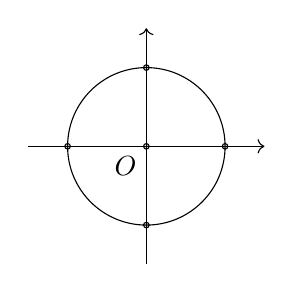
\begin{tikzpicture}[scale=1.0]
      \coordinate(O) at (0,0);
      \coordinate(X1)at(-1,0);\coordinate(X2)at(1,0);
      \coordinate(Y1)at(0,-1);\coordinate(Y2)at(0,1);
      \tkzDrawPoints(O,X1,X2,Y1,Y2)\node[below left]at(O){$O$};
      \draw(O)circle(1);
      \draw[->](-1.5,0)--(1.5,0);
      \draw[->](0,-1.5)--(0,1.5);
    \end{tikzpicture}
  \end{center}
  容易得到单位圆上点的实部的表达式为
  \begin{align*}
        & \mathrm{Re}\left( e^{i(\alpha + \beta + \gamma)}\right) \\
    ={} & \cos\alpha\cos\beta\cos\gamma - \cos\alpha\sin\beta\sin\gamma
          - \sin\alpha\cos\beta\sin\gamma - \sin\alpha\sin\beta\cos\gamma\\
  \end{align*}
  类似定理~\ref{th:tan-x+y+z=k},若$\cos\alpha, \cos\beta, \cos\gamma$均不为0,即$\alpha, \beta, \gamma$均不为$\pi/2$的奇数倍时,有
  \begin{align*}
    \frac{\mathrm{Re}\left( e^{i(\alpha + \beta + \gamma)}\right)}{\cos\alpha\cos\beta\cos\gamma}
    ={} 1 - \tan\alpha\tan\beta - \tan\beta\tan\gamma - \tan\gamma\tan\alpha
  \end{align*}
  取单位圆与虚轴的两个交点,即$\alpha + \beta + \gamma$是$\pi/2$的奇数倍,此两点的实部为0,从而
  \begin{align*}
    \alpha + \beta + \gamma = (2k + 1)\frac\pi2
    \iff & e^{i(\alpha + \beta + \gamma)} = \pm i 
    \iff \mathrm{Re}\left(e^{i(\alpha + \beta + \gamma)}\right) = 0\\
    % \iff & 1 - \tan\alpha\tan\beta - \tan\beta\tan\gamma - \tan\gamma\tan\alpha = 0\\
    \iff & \tan\alpha\tan\beta + \tan\beta\tan\gamma + \tan\gamma\tan\alpha = 1\qedhere\\
  \end{align*}
\end{example}

\begin{example}[几何证明]若$\alpha,\beta,\gamma$是锐角且$\alpha+\beta+\gamma=\pi$,则
  \begin{align*}
    \tan\alpha + \tan\beta + \tan\gamma = \tan\alpha \tan\beta \tan\gamma
  \end{align*}

  如图,作出$\alpha,\beta,\gamma$,并通过其中一条垂线作出长方形,令长方形的底长度为$\tan\alpha\tan\beta\tan\gamma$。依次求解图中4个三角形,则可以求出图中各线段长度,再由上下底边相等可得。
  \begin{center}
    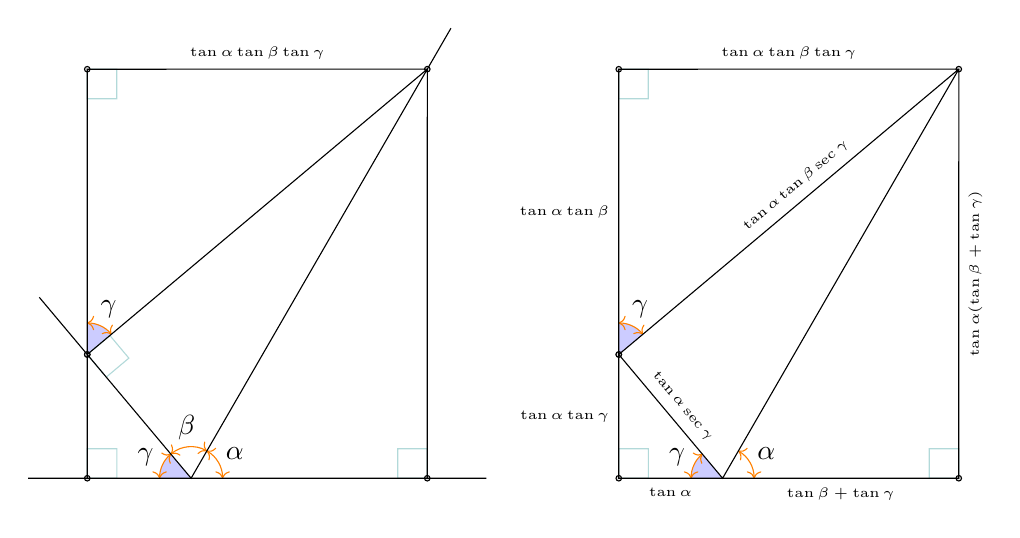
\begin{tikzpicture}[scale=1.5]
      % \begin{scope}
      %   \coordinate(O)at(0,0);\coordinate(A)at(1,0);\coordinate(B)at(60:2);\coordinate(C)at(130:2);\coordinate(D)at(-1,0);
      %   \draw(-2,0)--(2,0) (B)--(O)--(C);
      %   \draw pic["$\alpha$",<->,draw=orange,angle eccentricity=1.6,angle radius=.4cm]{angle=A--O--B};
      %   \draw pic["$\beta$",<->,draw=orange,angle eccentricity=1.6,angle radius=.4cm]{angle=B--O--C};
      %   \draw pic["$\gamma$",<->,draw=orange,angle eccentricity=1.6,angle radius=.4cm]{angle=C--O--D};
      % \end{scope}

      \begin{scope}[shift={(0,0)}]
        \coordinate(O)at(0,0);\coordinate(A)at(1,0);\coordinate(B)at(60:4);\coordinate(C)at(130:2);\coordinate(D)at(-1,0);
        \coordinate(E)at($(O)!(B)!(C)$);\coordinate(F)at($(D)!(E)!(O)$);
        \coordinate(G)at($(A)!(B)!(O)$);\coordinate(H)at($(F)!(B)!(E)$);
        
        \draw pic["$\alpha$",<->,draw=orange,angle eccentricity=1.6,angle radius=.4cm]{angle=A--O--B};
        \draw pic["$\beta$",<->,draw=orange,angle eccentricity=1.6,angle radius=.4cm]{angle=B--O--C};
        \draw pic["$\gamma$",<->,draw=orange,angle eccentricity=1.6,angle radius=.4cm,fill=blue!20]{angle=C--O--D};
        \draw pic["$\gamma$",<->,draw=orange,angle eccentricity=1.6,angle radius=.4cm,fill=blue!20]{angle=B--E--H};

        \foreach \x/\y/\z in{B/E/O,E/F/O,B/G/O,B/H/E}{
          \tkzMarkRightAngle[help lines](\x,\y,\z)
        }
        \tkzDrawPoints(E,F,G,B,H,E)

        % \draw(-.9,0)--(1.4,0) (B)--(O)--(C);
        \draw(E)--(F)--(O)
                --(G)
                --(B)--(H)node[midway,above]{\tiny $\tan\alpha\tan\beta\tan\gamma$}
                --(E)--(B);
        \draw(F)--($(F)-(.5,0)$) (G)--($(G)+(.5,0)$) ($1.1*(B)$)--(O)--(C);
      \end{scope}

      \begin{scope}[shift={(4.5,0)}]
        \coordinate(O)at(0,0);\coordinate(A)at(1,0);\coordinate(B)at(60:4);\coordinate(C)at(130:2);\coordinate(D)at(-1,0);
        \coordinate(E)at($(O)!(B)!(C)$);\coordinate(F)at($(D)!(E)!(O)$);
        \coordinate(G)at($(A)!(B)!(O)$);\coordinate(H)at($(F)!(B)!(E)$);
        
        \draw pic["$\alpha$",<->,draw=orange,angle eccentricity=1.6,angle radius=.4cm]{angle=A--O--B};
        % \draw pic["$\beta$",<->,draw=orange,angle eccentricity=1.6,angle radius=.4cm]{angle=B--O--C};
        \draw pic["$\gamma$",<->,draw=orange,angle eccentricity=1.6,angle radius=.4cm,fill=blue!20]{angle=C--O--D};
        \draw pic["$\gamma$",<->,draw=orange,angle eccentricity=1.6,angle radius=.4cm,fill=blue!20]{angle=B--E--H};

        \foreach \x/\y/\z in{% B/E/C,
          E/F/O,B/G/O,B/H/E}{
          \tkzMarkRightAngle[help lines](\x,\y,\z)
        }
        \tkzDrawPoints(E,F,G,B,H,E)

        % \draw(-.9,0)--(1.4,0) (B)--(O)--(C);
        \draw(E)--(F)node[midway,left]{\tiny $\tan\alpha\tan\gamma$}
                --(O)node[midway,below]{\tiny $\tan\alpha$}
                --(G)node[midway,below]{\tiny $\tan\beta+\tan\gamma$}
                --(B)node[midway,sloped,below]{\tiny $\tan\alpha(\tan\beta+\tan\gamma)$}
                --(H)node[midway,above]{\tiny $\tan\alpha\tan\beta\tan\gamma$}
                --(E)node[midway,left]{\tiny $\tan\alpha\tan\beta$}
                --(B)node[pos=.55,sloped,above]{\tiny $\tan\alpha\tan\beta\sec\gamma$};
        % \draw(F)--($(F)-(1,0)$) (G)--($(G)+(1,0)$) ($1.1*(B)$)--(O);
        \draw(E)--(O)node[midway,sloped,above]{\tiny $\tan\alpha\sec\gamma$} --(B);

        % \draw[help lines,->]($.5*(E)$)--(0,-1);\node[below]at(0,-1){\tiny $\tan\alpha\sec\gamma$};
      \end{scope}
    \end{tikzpicture}
  \end{center}
\end{example}

\section{完全平方数}
\label{sec:perfect-squares}

\begin{example}[1953 \kurschak]
  $\forall n\in\mathcal{Z}^+$,若正整数$d$整除$2n^2$,则$n^2+d$不是完全平方数。
\end{example}

\hints 反证。令$d=2n^2/k$,若$n^2+d=n^2+2n^2/k=m^2$,则$(mk)^2=n^2(k^2+2k)$,从而$k^2+2k$也是一个完全平方数。然而$k^2<k^2+2k<k^2+2k+1=(k+1)^2$,即$k^2+2k$位于两个相邻的完全平方数之间,从而不能是完全平方数,矛盾。

\section{抽屉原理}
\label{sec:pigeonhole-principle}

\begin{theorem}[抽屉原理]
  若有$n$个笼子和$kn+1$只鸽子,所有的鸽子都被关在鸽笼里,那么至少有一个笼子有至少$k+1$只鸽子。
\end{theorem}

抽屉原理,也叫鸽笼原理,鴿巢原理(Pigeonhole Principle)。

\begin{proof}
  反证法,若每个笼子最多有不超过$k$个鸽子,那么所有笼子鸽子总数不超过$kn$个,与原来有$kn+1$个鸽子矛盾。
\end{proof}

当$k=1$时,是抽屉原理最觉的情况:若有$n$个笼子和$n+1$只鸽子,所有的鸽子都被关在鸽笼里,那么至少有一个笼子有至少$2$只鸽子。

\think 若上面$n+1$只鸽子换成$n+1,n+2,\cdots$是否成立?

\begin{example}
  普遍认为成人的头发数量约在10万左右,那么对于深圳的常住人口(按2018年2180万算),基本可以肯定有人有相同的头发数。
\end{example}

\begin{proof}
  按头发数做鸽笼,按统计数据成人头发约为10万左右,可认为深圳常住人口的头发数量都小于等于2000万根。按抽屉原理可得。
\end{proof}

\begin{example}
  在$1,2,\cdots,100$里任意选51个数,总能在这选出来的数中找到两个互质数。
\end{example}

\begin{proof}
  将100个数按$(1,2), (3,4), \cdots, (99,100)$分为50组,则选51个数总有两个落到同一组中,而同一组的两数互质,从而得证。
\end{proof}

\begin{question}
  在$1,2,\cdots,100$里任意选51个数,总能在这选出来的数中找到两个,使得其中一个被另一个整除。
\end{question}
\hints $\forall a\in\mathcal{Z}^+$,存在奇数$k$及整数$n$,使得$a=k\cdot 2^n$。对所有整数按$k$分类。

\begin{example}
  在任意9个两两不等的实数中,总能选出两个,设其为$a,b$,满足以下条件
  \begin{align*}
    0 < \frac{a-b}{1+ab} < \sqrt2 -1
  \end{align*}
\end{example}

\begin{proof}
  联想公式
  \begin{align*}
    \tan(\alpha-\beta)=\frac{\tan\alpha-\tan\beta}{1+\tan\alpha\tan\beta}
  \end{align*}

  而$\tan(x)$的周期是$(-\pi/2, \pi/2]$,将区间8等份(让9个数总有两个落入其中一份)为以下8个区间
  \begin{align*}
    (-\frac\pi2, -\frac{3\pi}8], (-\frac{3\pi}8, -\frac\pi4], \cdots, (\frac{3\pi}8, \frac\pi8]
  \end{align*}

  $\forall a, \exists\hat a\in(-\pi/2, \pi/2], s.t. \tan\hat a = a$,从而任意9个实数,总存在两个,记为$a,b$,存在$\hat a, \hat b$落在上述8个区间中的同一个,且有$a=\tan\hat a, b=\tan\hat b$。不妨设$a>b$,从而$0<\hat a-\hat b<\pi/8$,由$\tan(x)$在上述每个区间中均为严格单调递增,有
  \begin{align*}
             & 0 < \tan(\hat a - \hat b) < \tan\frac\pi8\\
    \implies & 0 < \frac{a - b}{1+ab} < \sqrt2 - 1
  \end{align*}
\end{proof}


\begin{question}[XLI Mathematical Olympiad in Poland]
  一个三角形可以放置在一个单位正方形内,且存在一种放置方法使得正方形的中心不在三角形内。那么该三角形有一条边长小于1。
\end{question}

\hints 将正方形划分几份,使得三角形至少有两个顶点落在某份中。

%%%%%%%%%%%%%%%%%%%%
%%% Questions
%%%%%%%%%%%%%%%%%%%%
\begin{question}
  从$1,2,\cdots,100$中任意取11个数字,那么这11个数字组成的集合中,总存在两个不相交的非空子集,其元素之和相等。
\end{question}

\hints 11个元素组成的集合,其非空真子集总共有$2^{11}-2=2046$个,而1到100取10个数字(\think 为什么取10个而不是11个)其和最大值为$91+92+\cdots+100=955$。

\begin{question}
  在三维空间中任意选取9个坐标都是整数的点。证明这连接9个点而形成的线段中至少包含另外一个坐标为整数的点
\end{question}

\begin{question}
  任意六个人中,以下两个结论总有一个成立:
  \begin{enumerate}
  \item 其中有三人互相认识。
  \item 其中有三人互相不认识。
  \end{enumerate}
\end{question}

\hints 相当于正六边形的六个顶点用两种颜色的线段两两连接起来,则这些线段组合的三角形中,总存在一个同色的三角形。

\begin{question}
  任意一个16位的正整数的数字所组成的数字串中,总存在一个子串,其数字的乘积是一个完全平方数。
\end{question}

\hints 若16位数中含有数字$0,1,4,9$,那么取这个数字本身组成的子串即可,从而只需考虑由数字$2,3,5,6,7,8$组成的16位数。由于
\begin{align*}
  6 = 2\times 3,\quad 8=2^3
\end{align*}
从而任意一个子串各数字的乘积可以写成如下形式
\begin{align*}
  2^a \times 3^b \times 5^c \times 7^d
\end{align*}
若$a,b,c,d$都是偶数,那么这个子串数字的乘积就是完全平方数。而$a,b,c,d$的奇偶组合数总共有$2^4=16$种,即
\begin{align*}
  \text{(奇奇奇奇)},\quad \text{(奇奇奇偶)},\quad \text{(奇奇偶奇)},\quad \text{(奇奇偶偶)}\\
  \text{(奇偶奇奇)},\quad \text{(奇偶奇偶)},\quad \text{(奇偶偶奇)},\quad \text{(奇偶偶偶)}\\
  \text{(偶奇奇奇)},\quad \text{(偶奇奇偶)},\quad \text{(偶奇偶奇)},\quad \text{(偶奇偶偶)}\\
  \text{(偶偶奇奇)},\quad \text{(偶偶奇偶)},\quad \text{(偶偶偶奇)},\quad \text{(偶偶偶偶)}
\end{align*}

从而至少需要构造17种选取方式。记16位数各数字按顺序分别为$x_1,x_2,\cdots,x_{16}$,令
\begin{align*}
  F(k) =
  \begin{cases}
    1 = 2^0 \times 3^0 \times 5^0 \times 7^0 & k=0\\
    \prod_{i=1}^k x_i = 2^{a_k} \times 3^{b_k} \times 5^{c_k} \times 7^{d_k},&k=1,2,\cdots,16
  \end{cases}
\end{align*}
则$F(0),F(1),\cdots,F(16)$这17个数中至少有两个,其$a,b,c,d$的奇偶性组合相同,不妨记为$F(k_1),F(k_2)$,且$k_1<k_2$,从而$F(k_2)/F(k_1)$是完全平方数,从而两个数对应的子串,长串中拿掉短串部分,其数字乘积即为完全平方数。


\chapter{Buffalo Way}
\label{chap:buffalo-way}

Buffalo Way(BW)是一种方法,通常用于解决对称性问题,对于$x_1\le x_2\le x_3\le \cdots\le x_n$,令
\begin{align*}
  x_1&=y_1\\
  x_2&=y_1+y_2\\
  x_3&=y_1+y_2+y_3\\
  \cdots&\cdots\\
  x_n&=y_1+y_2+y_3+\cdots+y_n
\end{align*}
其中除$y_1$外$y_2,y_3,\cdots y_n$均为非负数。代入原问题换元求解。

\begin{example}
  证明:若$0\le a\le b\le c$,则$(a+b)(a+c)^2\ge 6abc$。
\end{example}
\begin{proof}
  应用Buffalo Way,令$a=x$, $b=x+y$, $c=x+y+z$,其中$x$,$y$,$z$均为非负数。代入,有
  \begin{align*}
    &(a+b)(a+c)^2\ge 6abc\\
    \iff& (2x+y)(2x+y+z)^2\ge 6x(x+y)(x+y+z)
  \end{align*}
  化简后上式等价于
  \begin{align*}
    2x^3+2x^2z+2xyz+2xz^2+y^3+2y^2z+yz^2\ge 0
  \end{align*}
  由于$x,y,z$非负,上式显然成立,且等号成立时当且仅当以下各式同时满足
  \begin{align*}
    2x^3&=0,    &2x^2z&=0,  &2xyz&=0,  &2xz^2&=0\\
    y^3&=0,     &2y^2z&=0,  &yz^2&=0   &     &
  \end{align*}
  即$x=y=0$,$z$任意。即等号成立当且仅当$a=b=0$。
\end{proof}

\begin{example}
  证明:对于正数$x,y,z$,有
  \begin{align*}
    \sum_{\mathrm{cyc}} \frac{x^4}{8x^3+5y^3}\ge\frac{x+y+z}{13}
  \end{align*}
  其中$\sum\limits{\mathrm{cyc}}$表示轮换求和,对上式的$x$,$y$和$z$作轮换,则有
  \begin{align*}
    \sum_{\mathrm{cyc}}\frac{x^4}{8x^3+5y^3} \implies
    \begin{cases}
      \dfrac{x^4}{8x^3+5y^3} \xRightarrow{x\leftarrow x, y\leftarrow y} \dfrac{x^4}{8x^3+5y^3} \\
      \dfrac{x^4}{8x^3+5y^3} \xRightarrow{x\leftarrow y, y\leftarrow z} \dfrac{y^4}{8y^3+5z^3} \\
      \dfrac{x^4}{8x^3+5y^3} \xRightarrow{x\leftarrow z, y\leftarrow x} \dfrac{z^4}{8z^3+5x^3}
    \end{cases}%
  \end{align*}
  上面三式相加,可得:
  \begin{align*}
    \sum_{\mathrm{cyc}} \frac{x^4}{8x^3+5y^3} = \frac{x^4}{8x^3+5y^3}
    + \frac{y^4}{8y^3+5z^3}
    + \frac{z^4}{z^3+5x^3}
  \end{align*}
\end{example}
\begin{proof}
  应用BW,不妨设$0<x\le y\le z$,且$y=x+u$,$z=x+u+v$,代入。{\color{red}非常繁琐!如果想锻炼计算能力,可以一试;如果是竞赛题,基本可放弃此方法,需另辟蹊径。}
\end{proof}

\begin{example}
  证明:对任意正数$x,y,z$,有
  \begin{align*}
    \sum_{\mathrm{cyc}}\frac1{(x-y)^2}\equiv\frac1{(x-y)^2}+\frac1{(y-z)^2}+\frac1{(z-x)^2}\ge\frac4{xy+yz+zx}
  \end{align*}
\end{example}
\begin{proof}
  不失一般性,不妨设$0<x\le y\le z$,且$y=x+u,z=x+u+v$,其中$u,v$非负。代入经过繁琐的计算可得。
\end{proof}


可以看出,应用BW时其过程非常直观,不需要过多的思考,但伴随而来的缺点是通常会涉及比较繁琐的计算。BW方法并不是时时都有效,比如下面这一题。
\begin{example}
  证明:对于正数$x,y,z$,有
  \begin{align*}
    \sum_{\mathrm{cyc}} \frac{x^3}{13x^2+5y^2}\ge\frac{x+y+z}{18}
  \end{align*}
\end{example}


% \chapter{不等式}
% \label{chap:inequality}


\section{基本不等式}
\label{sec:basic-inequalities}

\begin{definition}[算术平均数,Arithmetic Means, AM)]
  $\forall x_i$,下式称为其代数平均数
  \begin{align*}
    A_n\equiv\frac{\sum\limits_{i=1}^{n} x_i}{n}
    =\frac{x_1+x_2+x_3+\cdots+x_n}{n}
  \end{align*}
\end{definition}

\begin{definition}[几何平均数, Geometric Means, GM]
  $\forall x_i\ge0$,下式称为其几何平均数
  \begin{align*}
    G_n\equiv\sqrt[n]{\prod_{i=1}^{n}x_i}
    =\sqrt[n]{x_1 x_2 x_3\cdots x_n}
  \end{align*}
\end{definition}

\begin{definition}[调和平均数,Harmonic Means, HM]
  $\forall x_i\ge0$,下式称为其调和平均数
  \begin{align*}
    H_n\equiv\frac{n}{\sum\limits_{i=1}^{n}\dfrac1{x_i}}
    =\frac{n}{\dfrac1{x_1}+\dfrac1{x_2}+\cdots+\dfrac1{x_n}}
    =\frac{1}{\dfrac{\dfrac1{x_1}+\dfrac1{x_2}+\cdots+\dfrac1{x_n}}{n}}
  \end{align*}
\end{definition}

\begin{definition}[平方平均数,Quadratic Mean,QM]
  $\forall x_i$,下式称不其平方平均数
  \begin{align*}
    Q_n\equiv\sqrt{\dfrac{\sum\limits_{i=1}^n x_i^2}{n}}
    =\sqrt{\frac{x_1^2+x_2^2+\cdots+x_n^2}{n}}
  \end{align*}
  平均平方数也称为\term{均方根}(Root Mean Square)。
\end{definition}

若令
\begin{align*}
  \varphi(x_1,x_2,\cdots,x_n;p)\equiv\left(\frac{\sum_{i=1}^{n} x_i^p}{n} \right)^{\frac1p}
  =\left( \frac{x_1^p + x_2^p + \cdots + x_n^p}{n} \right)^{\frac1p}
\end{align*}
则显然有
\begin{align*}
  H_n \equiv \mathrm{HM}(x_1,x_2,\cdots,x_n)&=\varphi(x_1,x_2,\cdots,x_n;-1)\\
  A_n \equiv \mathrm{AM}(x_1,x_2,\cdots,x_n)&=\varphi(x_1,x_2,\cdots,x_n;1)\\
  Q_n \equiv \mathrm{QM}(x_1,x_2,\cdots,x_n)&=\varphi(x_1,x_2,\cdots,x_n;2)
\end{align*}

思考:是否能推出固定$x_1,x_2,\cdots,x_n$,则$\varphi(x_1,x_2,\cdots,x_n;p)$关于$p$是递增函数?若可以,则显然有$H_n\le A_n\le Q_n$。

\begin{theorem}[HM-GM-AM-QM]
  任意正数序列$x_i$,有
  \begin{align*}
    H_n\le G_n\le A_n\le Q_n
  \end{align*}
\end{theorem}
\begin{figure}[htbp]
  \centering
  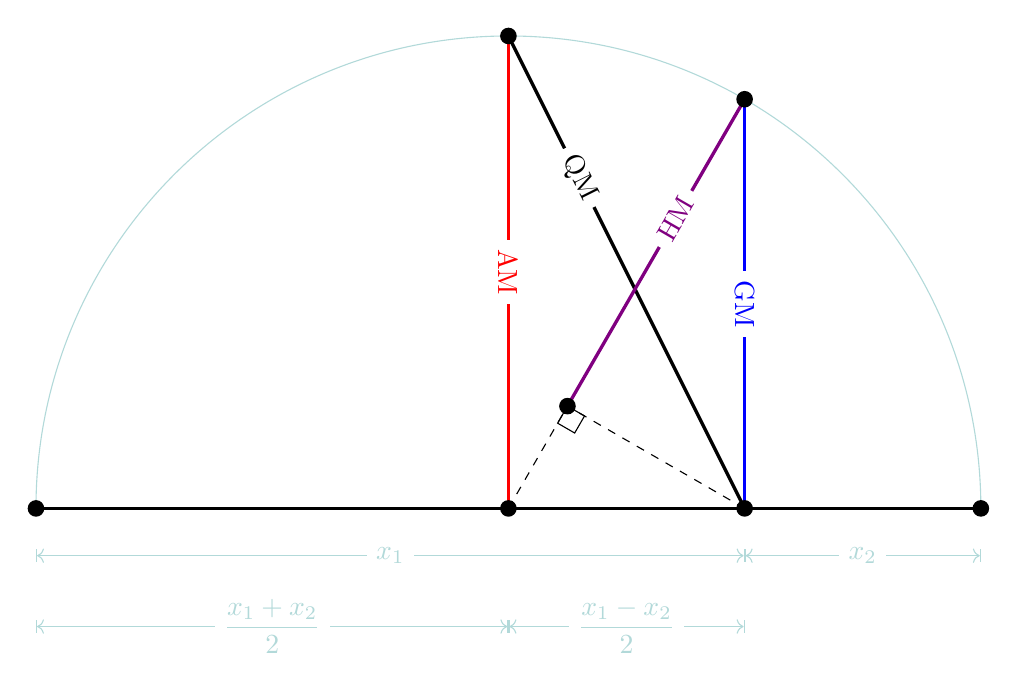
\begin{tikzpicture}[scale=1.0]
    \draw[help lines](-6,0)--(6,0) arc (0:180:6);
    \draw[help lines,|<->|](-6,-0.6)--(3,-0.6) node[midway,fill=white]{$x_1$};
    \draw[help lines,|<->|](3,-0.6)--(6,-0.6) node[midway,fill=white]{$x_2$};
    \draw[help lines,|<->|](-6,-1.5)--(0,-1.5)node[midway,fill=white]{$\dfrac{x_1+x_2}2$};
    \draw[help lines,|<->|](0,-1.5)--(3,-1.5)node[midway,fill=white]{$\dfrac{x_1-x_2}2$};
    \coordinate (G) at (60:6);
    \coordinate (H) at (60:1.5);
    \tkzDefPoint(3,0){C}
    \tkzDefPoint(0,0){O}
    \tkzMarkRightAngle[draw,fill=white](O,H,C)
    \draw[very thick, blue](G)--(C) node[sloped,midway,fill=white]{GM};
    \draw[very thick, red](0,6)--(0,0) node[midway,sloped,fill=white]{AM};
    \draw[very thick](0,6)--(C) node[sloped,pos=0.3,fill=white]{QM};
    \draw[very thick, violet](H)--(G) node[sloped,pos=0.61,fill=white]{HM};
    \draw[very thick](-6,0)--(6,0);
    \fill (-6,0) circle(3pt);
    \fill (C) circle(3pt);
    \fill (6,0) circle(3pt);
    \fill (G) circle(3pt);
    \fill (H) circle(3pt);
    \fill (0,6) circle(3pt);
    \fill (O) circle(3pt);
    \draw[dashed](0,0)--(H);
    \draw[dashed](3,0)--(H);
  \end{tikzpicture}
  \caption{$n=2$时HM,GM,AM,QM的几何示意}
  \label{fig:HM-GM-AM-QM}
\end{figure}

\begin{lemma}\label{lemma:b-1-a}
  若$b\le1\le a$,则$ab\le a+b-1$。
\end{lemma}
\begin{proof}
  由$0\le (a-1)(1-b)=a+b-ab-1$可得。此引理比较重要,被应用到很多不等式的证明过程中。
\end{proof}

\begin{lemma}\label{lemma:product-ai-ge-n}
  $\forall a_i>0$,若满足$\prod_{i=1}^n a_i=1$,则以下不等式成立
  \begin{align}
    \sum_{i=1}^n a_i\ge n
  \end{align}
  当且仅当$a_1=a_2=\cdots=a_n=1$时上述等号成立。
\end{lemma}
\begin{proof}
  对$n$作数学归纳。当$n=1$时显然。当$n\ge2$时,不妨对$a_i$重新排列使得$a_1\equiv\max(a_1,a_2,\cdots,a_n)\ge1$,$a_2\equiv\min(a_1,a_2,\cdots,a_n)\le1$,那么以下$n-1$个数的序列
  \begin{align*}
    a_1a_2, a_3, a_4, \cdots, a_n
  \end{align*}
  满足$n-1$的情况,从而有
  \begin{align*}
    a_1a_2 + a_3+ a_4+ \cdots + a_n &\ge n-1
  \end{align*}
  当且仅当$a_1a_2=a_3=a_4=\cdots=a_n=1$时等号成立,又由引理\ref{lemma:b-1-a},$a_1+a_2 - 1\ge a_1a_2$,其中等号当且仅当$a_1=1$或者$a_2=1$时成立。代入后有
  \begin{align*}
    (a_1 + a_2 - 1) + a_3+ a_4+ \cdots + a_n &\ge n-1\\
    a_1 + a_2 + \cdots + a_n\ge n
  \end{align*}
  其中等号成立,当且仅当以下两个条件同时满足:
  \begin{enumerate}
  \item $a_1a_2=a_3=a_4=\cdots=a_n=1$
  \item $a_1=1$或者$a_2=1$
  \end{enumerate}
  由此条件可知当且仅当所有的$a_i$都等于1时等号成立。
\end{proof}

下面证明AM-GM不等式。
\begin{proof}
  令$g\equiv\sqrt[n]{\prod\limits_{i=1}^n a_i}$,对序列
  \begin{align*}
    \frac{a_1}{g}, \frac{a_2}{g}, \frac{a_3}{g}, \cdots, \frac{a_n}{g}
  \end{align*}
  应用引理\ref{lemma:product-ai-ge-n},有
  \begin{align*}
    \frac{a_1}{g} + \frac{a_2}{g} + \frac{a_3}{g} + \cdots + \frac{a_n}{g}&\ge n\\
    \frac{a_1 + a_2 + a_3 + \cdots + a_n}{n}&\ge g = \sqrt[n]{a_1a_2a_3\cdots a_n} \qedhere
  \end{align*}
\end{proof}

对于三角形,HM还有以下几何意义:
\begin{example}
  对任意三角形,其内切圆的半径是三角形三条高长度的调和平均值的三分之一,即
  \begin{align*}
    r=\frac13 HM(h_a,h_b,h_c)
  \end{align*}
\end{example}
\begin{proof}
  尝试用面积来解,如图~\ref{fig:incircle}所示设三边边长分别是$a,b,c$,
  其对应的高分别为 $h_a, h_b, h_c$,则三角形面积$S=\frac12
  ah_a = \frac12 bh_b = \frac12 ch_c$,同样有$S=\frac12 r(a+b+c)$,从而
  \begin{align*}
    & S = \frac12 r\left( \frac{2S}{h_c} +\frac{2S}{h_a} + \frac{2S}{h_b} \right)
    \quad \implies\quad  r=\frac{1}{\dfrac1{h_a} + \dfrac1{h_b} + \dfrac1{h_c}} \qedhere
  \end{align*}
\end{proof}

\begin{figure}[htbp]
  \centering
  \begin{tikzpicture}[scale=1]
    \tkzDefPoint[label=below left:$A$](0,0){A}
    \tkzDefPoint[label=below right:$B$](6,0){B}
    \tkzDefPoint[label=above:$C$](5,5){C}
    
    \tkzDefCircle[in](A,B,C)\tkzGetPoint{I}\tkzGetLength{rIN}
    \tkzDrawCircle[R](I,\rIN pt);
    \tkzDrawSegments(A,B B,C C,A)
    \tkzDrawSegments[dashed](I,A I,B I,C)
    \tkzDrawCircle[fillstyle=solid,R](I,2pt)

    \coordinate(IA) at ($(B)!(I)!(C)$);
    \coordinate(IB) at ($(C)!(I)!(A)$);
    \coordinate(IC) at ($(A)!(I)!(B)$);

    \tkzDrawSegments[dashed](I,IA I,IB I,IC)
    \tkzMarkRightAngle[color=blue](B,IC,I)
    \tkzMarkRightAngle[color=blue](C,IA,I)
    \tkzMarkRightAngle[color=blue](A,IB,I)
  \end{tikzpicture}
  \caption{三角形内切圆}
  \label{fig:incircle}
\end{figure}

\begin{example}
  若任意非负数$a,b,c$满足$(a+1)(b+1)(c+1)=8$,则$abc\le 1$。
\end{example}
\begin{proof}
  若$a,b,c$均非负,则由AM-GM不等式,有$a+1\ge 2\sqrt{a}$,从而
  \begin{align*}
    8=(a+1)(b+1)(c+1)\ge 2\sqrt{a}\times 2\sqrt{b} \times 2\sqrt{c}
  \end{align*}
  即$abc\le1$。当且仅当$a=b=c=1$时等号成立。
\end{proof}

上述条件不能扩展到任意实数,$a,b,c$一负两正或者三个都是负数,则显然$abc<0$;但对
于$a,b,c$两负一正,比如$a=-2,b=-2,c=7$,则$abc>1$。



\begin{question}\label{q:1/1+a+b}
  三个正数$a,b,c$的乘积是1,求证
  \begin{align*}
    \frac1{1+a+b} + \frac1{1+b+c} + \frac1{1+c+a} \le 1
  \end{align*}
  当且仅当$a=b=c=1$时等号成立。
\end{question}

先尝试猜测每一项的上界。
\begin{align*}
  1+a+b\ge 3\sqrt[3]{ab},\quad 1+b+c \ge 3\sqrt[3]{bc},\quad 1+c+a\ge 3\sqrt[3]{ca}
\end{align*}
从而
\begin{align*}
  \frac1{1+b+c} + \frac1{1+c+a} + \frac1{1+a+b} \le
  \frac13\left( \frac1{\sqrt[3]{ab}} + \frac1{\sqrt[3]{bc}} + \frac1{\sqrt[3]{ca}} \right)
\end{align*}
令$a\to0+, b\to 0+, c=\frac1{ab}$,则上式$\le$符号右边$\to+\infty$,从而没上界,此估计无用。

% 又任意正数$x,y$,有
% \begin{align*}
%   \sqrt{xy}\ge \frac2{\dfrac1x + \dfrac1y}%
%   % \implies  \frac1{xy}\le \frac2{\dfrac1{x^2} + \dfrac1{y^2}}
% \end{align*}

% 令$a_0=\sqrt[6]a, b_0=\sqrt[6]b, c_0=\sqrt[6]c$,代入,有
% \begin{align*}
%   \frac1{\sqrt[3]{ab}} = \frac1{\sqrt{a_0b_0}}\le \frac2{\dfrac1{a_0} + \dfrac1{b_0}}
%   =\frac{2a_0b_0}{a_0+b_0}
% \end{align*}
% 同理处理$\frac1{\sqrt[3]{bc}}$和$\frac1{\sqrt[3]{ca}}$,从而有
% \begin{align*}
%   \frac1{1+b+c} + \frac1{1+c+a} + \frac1{1+a+b} \le
%   \frac23 \left(
%   \frac{a_0b_0}{a_0+b_0} + \frac{b_0c_0}{b_0+c_0} + \frac{c_0a_0}{c_0+a_0} 
%   \right)
% \end{align*}
% 其中$a_0b_0c_0=1$,且上式当且仅当$a_0=b_0=c_0=1$时等号成立。{\color{red}往下似乎不好走了,尝试换个方法。}


\begin{lemma}
对任意$a,b,c\in\mathcal{R}$,有以下恒等式:
\begin{align*}
  (a+b+c)(ab+bc+ca)&=a^2b+a^2c+b^2c+b^2a+c^2a+c^2b + 3abc\\
                   &=(a+b)(b+c)(c+a)+abc
\end{align*}
\end{lemma}
\begin{proof}
  左右分别展开可得证。
\end{proof}

令$x=b+c, y=c+a, z=a+b$,代入有
\begin{align*}
  & \frac1{1+b+c}+\frac1{1+c+a}+\frac1{1+a+b}\le 1\\
  \iff & \underline{(1+x)(1+y)} + (1+y)(1+z) + (1+z)(1+x) \le \underline{(1+x)(1+y)(1+z)}\\
  \iff & \underline{z(1+x)(1+y)} - \underline{(1+y)(1+z)} - (1+z)(1+x) \ge 0\\
  \iff & \underline{zx(1+y)} - (1+y) - 1-x-z-\underline{zx}\ge 0\\
  \iff & zxy - 2 - (x+y+z)\ge 0\\
  \iff & (a+b)(b+c)(c+a) - 2 - 2(a+b+c)\ge 0\\
  \iff & (a+b+c)(ab+bc+ca) - abc -2(a+b+c)\ge 2 \quad(\text{把}abc=1\text{代入})\\
  \iff & (a+b+c)(ab+bc+ca-2)\ge 3
  % \iff & (1+c+a)(1+a+b) + (1+b+c)(1+a+b) + (1+b+c)(1+c+a) \le (1+b+c)(1+c+a)(1+a+b)\\
  % \iff & (b+c)(1+c+a)(1+a+b) - (1+b+c)(1+a+b) - (1+b+c)(1+c+a) \ge 0\\
  % \iff & (b+c)(c+a)(1+a+b) - (1+a+b) - (1+b+c)(1+c+a) \ge 0\\
  % \iff & (b+c)(c+a)(a+b) - (1+a+b) - (1+c+a) - (b+c) \ge 0\\
  % \iff & (b+c)(c+a)(a+b) - 2(1+a+b+c)\ge 0\\
  % \iff & cab+b^2c+a^2b+ab^2 +c^2a+bc^2+a^2c+abc - 2(1+a+b+c)\ge 0\\
  % \iff & b^2c+a^2b+ab^2 +c^2a+bc^2+a^2c - 2(a+b+c)\ge 0\\
  % \iff & (a+b+c)(ab+bc+ca)-3abc -2(a+b+c)\ge 0\\
  % \iff & (a+b+c)(ab+bc+ca-2)\ge 3
\end{align*}
而由AM-GM不等式,有$a+b+c\ge 3\sqrt[3]{abc}=3, ab+bc+ca\ge 3\sqrt[3]{ab\cdot bc\cdot ca}=3$,可得。


\begin{question}
  上题中能否推广到任意正整数$n$,若正数$a_1,a_2,\cdots,a_n$的乘积是$1$,且令$S$表示其和,即
  \begin{align*}
    S\equiv\sum_{i=1}^n a_i
  \end{align*}
  则有
  \begin{align*}
    \sum_{i=1}^n \frac{1}{1 - a_i + S}\le 1
  \end{align*}
  当且仅当$a_1=a_2=\cdots=a_n=1$时等号成立?
\end{question}

当$n=1$时,$a_1=1$,有
\begin{align*}
  \sum_{i=1}^n \frac{1}{1 - a_i + S} = \frac{1}{1} = 1
\end{align*}

当$n=2$时,由$a_1a_2=1$,代入后恒有
\begin{align*}
  \sum_{i=1}^n \frac{1}{1 - a_i + S} &= \frac{1}{1+a_2} + \frac1{1+a_1}\\
                                     &= \frac{1+a_1 + 1 + a_2}{(1+a_1)(1+a_2)}\\
                                     &=1
\end{align*}

当$n=3$时,由题\ref{q:1/1+a+b}已得证。若用引理\ref{lemma:product-ai-ge-n},有$S\ge 3$,从而
\begin{align*}
  \sum_{i=1}^n \frac{1}{1 - a_i + S} &\le \sum_{i=1}^n \frac{1}{1 - a_i + 3}\\
                                     &=   \sum_{i=1}^n \frac{1}{4 - a_i}\\
\end{align*}
{\color{red}上式可不一定,比如$a_i>4$呢?这方法不一定可行。}

用数学归纳法。设$n\le k$时成立,考虑$n=k+1$的情况。考虑数列$\{a_1,a_2,\cdots, a_{k-1}, a_ka_{k+1}\}$,共$k$个数,且其乘积为$1$,从而有
\begin{align*}
  \sum_{i=1}^{k} \frac{1}{1 - a_i' + S_{k+1}'}
\end{align*}
其中
\begin{align*}
  a_i'=
  \begin{cases}
    a_i &i=1,2,\cdots,k-1\\
    a_ka_{k+1} &i=k
  \end{cases} \quad
  S_{k+1}'= a_1+a_2+\cdots +a_{k-1} + a_ka_{k+1}
\end{align*}

%%%%%%%%%%%%%%%%%%%%%%%%%%%%%%%%%%%%%%%%
%%% Basic inequality examples
%%%%%%%%%%%%%%%%%%%%%%%%%%%%%%%%%%%%%%%%
\begin{example}
  证明对$\forall a,b,c\in\mathcal{R}$,有$a^2+b^2+c^2\ge ab+bc+ca$。
\end{example}
\begin{proof}
  由AM--GM不等式,有
\begin{align*}
  a^2+b^2\ge 2ab,\quad b^2+c^2\ge 2bc,\quad c^2+a^2\ge 2ca
\end{align*}
三式相加并除以2可得。该不等式可以推广:$\forall n>1, x_i\in\mathcal{R}(i=1,2,\cdots,n)$,有
\begin{align*}
  \sum_{i=1}^n x_i^2\ge \sum_{i=1}^n x_ix_{i+1}
\end{align*}
其中$x_{n+1}=x_1$。
\end{proof}

\begin{example}
  对任意非负数$a,b$及正整数$n\ge2$,有 $(n-1)a^n + b^n\ge na^{n-1}b$。
\end{example}
对序列$a^n,a^n,\cdots,a^n,b^n$(其中有$n-1$项$a^n$应用AM-GM不等式,有)
\begin{align*}
  \underbrace{a^n + a^n + \cdots + a^n}_{n-1\text{个}} + b^n \ge
  n\times \sqrt[n]{\left(a^n\right)^{n-1} b^n}
  = na^{n-1}b
\end{align*}
当$n=3,4,5$时,有
\begin{align*}
  2a^3 + b^3&\ge 3a^2b\\
  3a^4 + b^4&\ge 4a^3b\\
  4a^5 + b^5&\ge 5a^4b
\end{align*}

\begin{example}
  若正数$a,b,c$的乘积为$1$,求$ab+bc+ca$的极值。
\end{example}
\begin{proof}[提示]
\begin{align*}
  ab+bc+ca\ge 3\times\sqrt[3]{ab\cdot bc\cdot ca}=3\times\sqrt[3]{(abc)^2}=3
\end{align*}
当且仅当$a=b=c=1$时等号成立。另一方面,令$a=b=n,c=1/n^2$,则
\begin{align*}
  ab+bc+ca>ab=n^2\to+\infty (n\to+\infty)
\end{align*}
即$ab+bc+ca$无上界。
\end{proof}


\begin{example}
  若正数$a,b,c$的乘积为$1$,求$a+b+c$的极值。
\end{example}
\begin{align*}
  a+b+c\ge 3\times\sqrt[3]{abc}=3
\end{align*}
当且仅当$a=b=c=1$时等号成立。另一方面,令$a=b=n,c=1/n^2$,则
\begin{align*}
  a+b+c>a=n\to+\infty(n\to+\infty)
\end{align*}
即$a+b+c$无上界。

\begin{example}
  找出所有满足下列等式的实数$a,b,c,d$
  \begin{align*}
    a^2+b^2+c^2+d^2=a(b+c+d)
  \end{align*}
\end{example}

$\forall a,b,c,d\in\mathcal{R}$,有
\begin{align*}
  \left(\frac a2\right)^2\ge 0,\quad \left(\frac a2\right)^2 + b^2\ge ab,
  \quad \left(\frac a2\right)^2 + c^2\ge ac, \quad \left(\frac a2\right)^2 + d^2\ge ad
\end{align*}
四式相加,有
\begin{align*}
  a^2+b^2+c^2+d^2\ge a(b+c+d)
\end{align*}
当且仅当$a=0, \frac a2=b=c=d$时即$a=b=c=d=0$时成立。即原题只有$a=b=c=d=0$这一个解。

\begin{example}
  若正数$a,b,c$的平方和为1,求下式的最小值
  \begin{align*}
    S=\frac{a^2b^2}{c^2} + \frac{b^2c^2}{a^2} + \frac{c^2a^2}{b^2}
  \end{align*}
\end{example}

由
\begin{align*}
  \frac{a^2b^2}{c^2} + \frac{b^2c^2}{a^2}\ge 2b^2,\quad
  \frac{b^2c^2}{a^2} + \frac{c^2a^2}{b^2}\ge 2c^2,\quad
  \frac{c^2a^2}{b^2} + \frac{a^2b^2}{c^2}\ge 2a^2
\end{align*}
三式相加并除以2,有
\begin{align*}
  S\ge a^2+b^2+c^2=1
\end{align*}
当且仅当$\dfrac{a^2b^2}{c^2} = \dfrac{b^2c^2}{a^2} = \dfrac{c^2a^2}{b^2}$即$a=b=c=\frac1{\sqrt3}$时等号成立。


\begin{example}
  $x,y$是小于1的正数,则
  \begin{align*}
    \frac1{1-x^2} + \frac1{1-y^2} \ge \frac2{1-xy}
  \end{align*}
\end{example}
由$x+y\ge2\sqrt{xy}$,有
\begin{align*}
  \frac1{1-x^2} + \frac1{1-y^2} &\ge \frac2{\sqrt{(1-x^2)(1-y^2)}} &&\text{等号成立}\iff x=\pm y\\
  &=\frac2{\sqrt{1+x^2y^2-x^2-y^2}} \\
  &\ge \frac2{\sqrt{1+x^2y^2-2xy}} &&\text{等号成立}\iff x=y\\
  &=\frac2{\sqrt{(1-xy)^2}} \\
  &=\frac2{1-xy}
\end{align*}
当且仅当$x=y$时等号成立。

\begin{example}
  对任意非负数$a,b$,有
  \begin{align*}
    a^3+b^3\ge a^2b+ab^2
  \end{align*}
  推广:对任意非负数$a,b,c$,有
  \begin{align*}
    a^3+b^3+c^3\ge a^2b+b^2c+c^2a
  \end{align*}
  上述结论对任意$n>1$个非负数$a_1,a_2,\cdots,a_n$是否成立,即
  \begin{align*}
    \sum_{i=1}^n a_i^3\ge a_1^2a_2 + a_2^2a_3 + \cdots + a_{n-1}^2a_n + a_n^2a_1
  \end{align*}
\end{example}
由$a^3+b^3-a^2b-ab^2=a^2(a-b)+b^2(b-a)=(a-b)^2(a+b)\ge0$可得,当且仅当$a=b$时等号成立。

由$2a^3+b^3\ge3a^2b$,轮换$a,b,c$,有
\begin{align*}
  2a^3+b^3\ge3a^2b,\quad 2b^3+c^3\ge3b^2c,\quad 2c^3+a^3\ge3c^2a
\end{align*}
三式相加并除以3可得。

\begin{theorem}[Shapiro不等式,Shapiro's Cyclic Inequalities]
  $n$是正整数,序列$\{x_1,x_2,\cdots,x_n\}$是正数序列,则
  \begin{enumerate}
  \item 若$n$是正奇数且$3\le n\le 23$,则
    \begin{align*}
      \sum_{i=1}^{n} \frac{x_i}{x_{i+1} + x_{i+2}} \ge \frac{n}{2}  
    \end{align*}
    其中$x_{n+1} = x_1, x_{n+2} = x_2$。当且仅当$x_1=x_2=\cdots=x_n$时等号成立;

  \item 若$n$且正偶数且$4\le n\le 12$,则
    \begin{align*}
      \sum_{i=1}^{n} \frac{x_i}{x_{i+1} + x_{i+2}} \ge \frac{n}{2}  
    \end{align*}
    当且仅当$x_1=x_3=x_5=\cdots=x_{n-1}$且$x_2=x_4=x_6=\cdots=x_n$时等号成立;

  \item 若$n$是大于12的偶数或者是大于23的奇数,则存在正数序列$\{x_1,x_2,\cdots,x_n\}$,使得
    \begin{align*}
      \sum_{i=1}^{n} \frac{x_i}{x_{i+1} + x_{i+2}} < \frac{n}{2}  
    \end{align*}
  \end{enumerate}
\end{theorem}
\begin{proof}[说明]
  这里仅说明一下其证明历史。B.~A.~Troesch在1989年证明了(1),P.~J.~Bushell \& J.~B.~McLeod在2002年证明了(2),而(3)则是早在1979年就被 J.~L.~Searcy \& B.~A.~Troesch所证明。
\end{proof}

\begin{example}[Nesbitt不等式]
  对任意正数$a,b,c$,有
  \begin{align*}
    \frac{a}{b+c}+\frac{b}{c+a}+\frac{c}{a+b}\ge\frac32
  \end{align*}
\end{example}
\begin{proof}[提示]
  这是Shapiro不等式在$n=3$时的情形。有多种巧妙的证明方法。下面是其中三种。
  \begin{enumerate}
  \item 利用凸函数的Jensen不等式。记$S=a+b+c$,则
    \begin{align*}
      f(x)=\frac{x}{S-x}
    \end{align*}
    在$x\in[0,S)$上是凸的,应用Jensen不等式,则有
    \begin{align*}
      \frac{f(a) + f(b) + f(c)}{3}\ge f\left(\frac{a+b+c}{3}\right)=f\left(\frac{S}{3}\right)=\frac12
    \end{align*}
  \item 用换元法,消除难处理的分母。令$x=a+b,y=b+c,z=c+a$,则$x,y,z$是正数,且有
    \begin{align*}
      a=\frac{x-y+z}2,\quad b=\frac{x+y-z}2,\quad c=\frac{-x+y+z}2
    \end{align*}
    代入,有
    \begin{align*}
      \frac{a}{b+c}+\frac{b}{c+a}+\frac{c}{a+b}
      &= \frac{x-y+z}{2y} + \frac{x+y-z}{2z} + \frac{-x+y+z}{2x}\\
      &= \frac12\left(\frac{x+z}{y} + \frac{x+y}{z} + \frac{y+z}{x}\right)-\frac32\\
      &= \frac12\left( \underbrace{\left(\frac xy + \frac yx\right)}_{\text{应用AM--GM不等式}}
        +\left(\frac zy + \frac yz\right)
        +\left(\frac xz + \frac zx\right)
        \right)-\frac32\\
      &\ge \frac12\times ( 2 + 2 + 2) - \frac32=\frac32
      % &=\frac32
    \end{align*}
    当且仅当$\dfrac xy=\dfrac yx$, $\dfrac zy=\dfrac yz$, $\dfrac xz=\dfrac zx$即$x=y=z$时等号成立,亦即$a=b=c$时等号成立。

  \item 直接利用AM--HM不等式。由
    \begin{align*}
      & \frac{(a+b)+(b+c)+(c+a)}{3}\ge \frac{3}{\dfrac1{a+b}+\dfrac1{b+c}+\dfrac1{c+a}}\\
      \iff & \big[(a+b)+(b+c)+(c+a)\big]\left(\dfrac1{a+b}+\dfrac1{b+c}+\dfrac1{c+a}\right)\ge 9\\
      \iff & 2(a+b+c)\left(\dfrac1{a+b}+\dfrac1{b+c}+\dfrac1{c+a}\right)\ge 9\\
      \iff & 2\left(1+\dfrac{c}{a+b}+1+\dfrac{a}{b+c}+1+\dfrac{b}{c+a}\right)\ge 9
    \end{align*}
    展开可得。其等号成立的充要条件是$a+b=b+c=c+a$,即$a=b=c$。$\qedhere$
  \end{enumerate}
\end{proof}

\begin{question}
  证明Shapiro不等式在$n=4$时的情况,即对任意正数$a,b,c,d$,有
  \begin{align*}
    \frac{a}{b+c}+\frac{b}{c+d}+\frac{c}{d+a}+\frac{d}{a+b}\ge 2
  \end{align*}
\end{question}
% \begin{proof}[提示]
%   应用\ref{lemma:titu}的T2引理,有
%   \begin{align*}
%          &\frac{a}{b+c}+\frac{b}{c+d}+\frac{c}{d+a}+\frac{d}{a+b}\\
%     =\   &\frac{a^2}{a(b+c)}+\frac{b^2}{b(c+d)}+\frac{c^2}{c(d+a)}+\frac{d^2}{d(a+b)}\\
%     \ge\ &\dfrac{(a+b+c+d)^2}{a(b+c) + b(c+d) + c(d+a) + d(a+b)}
%   \end{align*}

%   \begin{align*}
%        & \frac{a}{b+c}+\frac{b}{c+d}+\frac{c}{d+a}+\frac{d}{a+b}\\
%     =\ & \left(\frac{a}{b+c}+\frac{c}{d+a}\right) + \left(\frac{b}{c+d}+\frac{d}{a+b}\right)\\
%     \ge\ & \dfrac{(a+c)^2}{a(b+c)+c(d+a)} + \dfrac{(b+d)^2}{b(c+d)+d(a+b)}\\
%     =\ & \dfrac{a^2+2ac+c^2}{ab+ac+cd+da}
%   \end{align*}
% \end{proof}

% 同样应用换元法简化分母,令$w=a+b$,$x=b+c$,$y=c+d$,$z=d+a$。先反求用$w$,$x$,$y$和$z$表示$a$:
% \begin{enumerate}
% \item 先看$w$,比$a$多了个$b$;
% \item $x$有$b$,$w-x=a-c$,又多减了个$c$;
% \item $y$里有$c$,$w-x+y=a+d$,则又多加了个$d$;
% \item $z$里有$d$,$w-x+y-z=2a$,多加了个$a$。
% \end{enumerate}
% 从而有$a=(w-x+y-z)/2$。类似地,有
% \begin{align*}
%   a&=\frac{w-x+y-z}2 & b&=\frac{x-y+z-w}2\\
%   c&=\frac{y-z+w-x}2 & d&=\frac{z-w+x-y}2
% \end{align*}
% 代入,有
% \begin{align*}
%      &\frac{a}{b+c}+\frac{b}{c+d}+\frac{c}{d+a}+\frac{d}{a+b}\\
%   =\ &\frac{w-x+y-z}{2x} + \frac{x-y+z-w}{2y} + \frac{y-z+w-x}{2z} + \frac{z-w+x-y}{2w}\\
%   =\ &\frac12\left( \frac{w+y-z}{x} + \frac{x+z-w}{y} + \frac{y+w-x}{z} + \frac{z+x-y}{w} - 4\right)
% \end{align*}
% 有负号,不能直接应用AM--GM不等式。代入继续化简,要证明的不等式等价于
% \begin{align*}
%        & \frac12\left( \frac{w+y-z}{x} + \frac{x+z-w}{y} + \frac{y+w-x}{z} + \frac{z+x-y}{w} - 4\right) \ge 2\\
%   \iff & \frac{w+y-z}{x} + \frac{x+z-w}{y} + \frac{y+w-x}{z} + \frac{z+x-y}{w} \ge 8\\
%   \iff & wyz(w+y-z) + xzw(x+z-w) + ywx(y+w-x) + zxy(z+x-y) \ge 8wxyz\\
%   \iff & w^2(yz-xz+xy) + x^2(wz-wy+yz) + y^2(
% \end{align*}


% {\color{red}似乎没用?}


\begin{question}
  证明:对任意正数$a,b,c$,有
  \begin{align*}
    \frac{a^3}{a^2+ab+b^2}+\frac{b^3}{b^2+bc+c^2}+\frac{c^3}{c^2+ca+a^2}
    \ge
    \frac{a+b+c}{3}
  \end{align*}
\end{question}

\begin{question}
  对任意正数$a_1,a_2,\cdots,a_n,b_1,b_2,\cdots,b_n$,有
  \begin{align*}
    \sum_{i=1}^n\frac{a_ib_i}{a_i+b_i}\le
    \frac{\sum\limits_{i=1}^n a_i \cdot \sum\limits_{i=1}^n b_i}
         {\sum\limits_{i=1}^n a_i + \sum\limits_{i=1}^n b_i}
  \end{align*}
\end{question}
对$n$用数学归纳法。

\begin{question}
  若$a_1,a_2,\cdots,a_n,b_1,b_2,\cdots,b_n$是正数,则
  \begin{align*}
    \sum_{i=1}^n \sqrt{a_ib_i}
    \le
    \sqrt{\sum_{i=1}^n a_i \cdot \sum_{i=1}^n b_i}
  \end{align*}
\end{question}
对$n$用数学归纳法。

\begin{question}
  对正数$a,b,c$,证明
  \begin{align*}
    \frac{5a^3-ab^2}{a+b} & \ge 3a^2-b^2\\
    \frac{5a^3-ab^2}{a+b} + \frac{5b^3-bc^2}{b+c} + \frac{5c^3-ca^2}{c+a} & \ge 2(a^2+b^2+c^2)
  \end{align*}
\end{question}
只需证明第一条即可,而第一条又等价于$2a^3+b^3\ge 3a^2b$。

\begin{question}
  对大于$2$的整数$n$,及非负数$x_1,x_2,\cdots,x_n$,若$x_1=0, x_n=1$,则存在整数$j\in[1,2,\cdots,n-1]$,使得
  \begin{align*}
    \left| x_{j-1} - 2x_j + x_{j+1} \right| \ge \frac{4}{n^2}
  \end{align*}
\end{question}
令$x_0=0,x_{n+1}=1$,且对$k=0,1,2,\cdots,n$,令$y_k=x_{k+1}-x_k$,则$y_0=y_n=0$,且$y_0+y_1+y_2+\cdots+y_n=1$。用反证法。假设对所有的$j=1,2,\cdots,n$,不等式不成立,从而有
\begin{align*}
  y_j - y_{j-1} \le \left| y_j-y_{j-1} \right| = \left| x_{j-1} - 2x_j + x_{j+1} \right| < \frac{4}{n^2}
\end{align*}
对$j=1,2,\cdots,k$加起来,则有
\begin{align*}
  y_k&=y_k-y_0=(y_1-y_0) + (y_2-y_1) + \cdots + (y_k-y_{k-1})\\
  &<\underbrace{\frac{4}{n^2}+\frac{4}{n^2}+\cdots+\frac{4}{n^2}}_{k\text{个}}\\
  &=\frac{4k}{n^2}
\end{align*}
同样$y_{j-1}-y_j<\frac{4}{n^2}$,加起来,有
\begin{align*}
  y_k&=y_{k}-y_n=(y_k-y_{k+1})+(y_{k+1}-y_{k+2})+\cdots+(y_{n-1}-y_{n})\\
  &<\underbrace{ \frac{4}{n^2}+\frac{4}{n^2}+\cdots+\frac{4}{n^2}}_{n-k\text{个}}\\
  &=\frac{4(n-k)}{n^2}
\end{align*}

若$n$是奇数,则
\begin{align*}
  1&=y_0+y_1+y_2+\cdots+y_n\\
  &=\left(y_1+y_1+\cdots+y_{\frac{n-1}2}\right)
  + \left(y_{\frac{n+1}2}+y_{\frac{n+1}2+1}+\cdots+y_n\right)\\
  & <\frac4{n^2}\left(
  \left(1+2+\cdots+\frac{n-1}2\right) +
  \left( \left(n-\frac{n+1}2\right) + \left(n-\frac{n+1}2-1\right) + \cdots + 1\right)
  \right)\\
  &=2\cdot\frac4{n^2}\left(1+2+\cdots+\frac{n-1}2\right)\\
  &=\frac8{n^2}\left( \left(1+\frac{n-1}2\right)\cdot\frac{n-1}2\cdot\frac12 \right)\\
  &=\frac{n^2-1}{n^2}<1
\end{align*}
矛盾。

若$n$是偶数,则
\begin{align*}
  1&=y_0+y_1+y_2+\cdots+y_n\\
  &=\left(y_1+y_1+\cdots+y_{\frac{n}2-1}\right)
  + \left(y_{\frac{n}2+1}+y_{\frac{n}2+2}+\cdots+y_n\right)
\end{align*}
剩余略。



\section{勾股数}
\label{sec:pythagorean_triples}

\begin{definition}[勾股数]
  若正整数$a,b,c$满足$a^2+b^2=c^2$,则称$a,b,c$为勾股数。
\end{definition}

勾股数也称为毕达哥拉斯三元组(Pythagorean Triples)。常见的勾股数有
\begin{align*}
  (3,4,5),\quad (5,12,13)
\end{align*}

\begin{property}
  $a,b,c$是勾股数,则
  \begin{enumerate}
  \item 若$a,b,c$三者的最大公约数是1,则$a,b,c$两两互质。
  \end{enumerate}
\end{property}

\begin{proof}
  略。
\end{proof}

\begin{definition}[Primitive Pythagorean Triples]
  勾股数$a,b,c$若两两互质,则称$a,b,c$为原始毕达哥拉斯三元组。
\end{definition}

\begin{lemma}
  $\forall n\in\mathcal{Z}^+, 4n+2$不是完全平方数。
\end{lemma}

\begin{proof}
  $4n+2=2(2n+1)$,而$2n+1$是奇数,即$4n+2$的因式分解中2的幂是奇数1,从而$4n+2$不可能是完全平方数。
\end{proof}

\begin{lemma}
  若$(a,b,c)$是原始毕达哥拉斯三元组,则$a,b$必是一奇一偶。
\end{lemma}

\begin{proof}
  首先排除$a,b$都是偶数的情况,否则$c$也是偶数,这样$(a,b,c)$不互质。再次排除$a,b$都是奇数的情况。假如$a,b$都是奇数,则$a^2\equiv b^2\equiv 1(\mod 4)$,从而$c^2\equiv 1 + 1\equiv 2(\mod 4)$不是一个完全平方数,矛盾。
\end{proof}

\begin{theorem}[Euclid's Formula]
  对任意整数$m>n>0$,则以下三元组是Pythagorean三元组
  \begin{align*}
    a=m^2-n^2,\quad b=2mn,\quad c=m^2+n^2
  \end{align*}
\end{theorem}

\begin{proof}
  略。按定义立得。
\end{proof}

\begin{theorem}\label{th:pythagorean-triples}
  若$(a,b,c)$是原始勾股数,且$a$是奇数,$b$是偶数,则存在两个互质且奇偶相反的整数$m>n>0$,使得
  \begin{align*}
    a=m^2-n^2,\quad b=2mn,\quad c=m^2+n^2
  \end{align*}
\end{theorem}

由此定理可知,原始勾股数都可以由Euclid公式生成。

\begin{proof}
  由于$b$是偶数,$a,c$都是奇数,从而$c\pm a$都是偶数,且有
  \begin{align*}
    \left(\frac b2\right)^2 = \frac{c+a}2\times\frac{c-a}2
  \end{align*}
  
  先证明$\dfrac{c\pm a}2$是互质的,否则存在整数$d>1$整除两数的和(等于$c$)与差(等于$a$),从而$c$和$a$有大于1的公约数$d$,与$(a,b,c)$两两互质矛盾。从而存在$m,n\in\mathcal{Z}^+$,使得
  \begin{align*}
    \frac{c+a}2=m^2,\quad \frac{c-a}2=n^2
  \end{align*}
  由上式得到$(a,b,c)$由$m,n$的表达式,后续过程以及请自行补充完整。

  关于$m,n$的奇偶性不同,首先由$m,n$互质排除两者都是偶数;若都是奇数,则由上面的表达式,$(a,b,c)$三者均为偶数,与$(a,b,c)$两两互质矛盾。从而$m,n$奇偶性不同。
\end{proof}


\begin{example}[1965 Putnam Exam.]
  面积的数值是其周长数值的两倍,且边长是整数的直角三角形总共只有3个。
\end{example}

\begin{proof}
  由定理\ref{th:pythagorean-triples},可设满足条件的三角形边长由下式给出
  \begin{align*}
    a = (m^2-n^2)d,\quad b=2mnd,\quad c=(m^2+n^2)d
  \end{align*}
  其中$d$是三边长的最大公约数,$m,n$满足定理\ref{th:pythagorean-triples}中的条件。再由面积的数值是周长数值的两倍,从而有
  \begin{align*}
    \frac12 \times (m^2-n^2)d\times 2mnd & = 2\left( (m^2-n^2)d + 2mnd + (m^2+n^2)d \right)\\
    \implies (m-n)nd & = 4
  \end{align*}
  由于$m-n$是奇数,从而$m-n=1$,又$n$是4的因数可取$1,2,4$,从而$m,n,d$的有以下三种组合
  \begin{align*}
    (2,1,4),\quad (3,2,2),\quad (5,4,1)
  \end{align*}
  此时对应的三角边长分别是
  \begin{align*}
    (12,16,20),\quad (10,24,26),\quad (9,40,41)
  \end{align*}
  即只有上述三种三角形。
\end{proof}

\begin{example}[1975 IMO]
  证明单位圆上任意两点间距离是有理数的点的集合可以有无限个元素。
\end{example}

\hints 令$A=(1,0),B=(-1,0),O$是原点。考虑
\begin{align*}
  \mathcal{P}\equiv\{p:AP=\frac{2(m^2-n^2)}{m^2+n^2}, BP=frac{4mn}{m^2+n^2}
\end{align*}
其中$m,n$满足定理\ref{th:pythagorean-triples},求$\mathcal{P}$中任意两点距离。

\begin{example}[Wiadom. Mat.(1955/56), pp.194-5, Polish]
  求$3^x+4^y=5^z$的所有正整数解。
\end{example}

\begin{proof}
  首先证明$z$是偶数。考虑模3的余数,有
  \begin{align*}
    1 \equiv 0 + 1^y \equiv 3^x + 4^y \equiv 5^z \equiv (-1)^z \tag*{$\pmod 3$}
  \end{align*}
  从而$z$必须是偶数,设$z=2w$,其中$w\in\mathcal{Z}^+$。从而有
  \begin{align*}
    3^x = 5^{2w} - 4^y = \left(5^w\right)^2 - \left(2^y\right)^2 = \left(5^w + 2^y\right)\left(5^w - 2^y\right)
  \end{align*}
  由于$(5^w + 2^y) + (5^w - 2^y) = 2\times 5^w$不能被3整除,从而$5^w + 2^y$和$5^w - 2^y$中有一个不能被3整除,再由上式,可知
  \begin{align*}
    5^w-2^y =1,\quad 5^w+2^y =3^x
  \end{align*}
  上式对3取模,有
  \begin{align*}
    (-1)^w - (-1)^y &= 1 \tag*{$\pmod 3$}\\
    (-1)^w + (-1)^y &= 0 \tag*{$\pmod 3$}\\
  \end{align*}
  从而$w$是奇数,$y$是偶数(请自行考虑)。若$y>2$,则
  \begin{align*}
     5^w\equiv 5^w+2^y \equiv 3^x \equiv 1\text{或者}3 \tag*{$\pmod 8$}
  \end{align*}
  又$w$是奇数,从而存在非负整数$u$,使得$w=2u + 1$,从而有
  \begin{align*}
    5^w \equiv 5^{2u + 1} \equiv 5\times 25^u \equiv 5\times (24 + 1)^u \equiv 5 \tag*{$\pmod 8$}
  \end{align*}
  两个结果矛盾,从而$y=2$。而由$5^w-2^y=1$,有$w=1$,从而$z=2w=2$,$x=2$。
\end{proof}

\chapter{平面几何五大模型}
\label{chap:five-models-in-geometry}

% \subsection{等积模型}
% \label{sec:same-volumne-model}

\begin{theorem}
  两个三角形若等底等高,则其面积相等。
\end{theorem}

此结论由三角形面积公式显然可得。

\begin{definition}[共角三角形]
  两三角形若有一个角相等或互补,则称这两个三角形为共同三角形。
\end{definition}

\begin{theorem}[共角定理,鸟头定理]
  共角三角形的面积比等于相等或互补的角的两夹边的乘积比。
\end{theorem}
\begin{proof}
  由三角形的另一面积公式$S=\dfrac12ab\sin C$,结论显然成立。
\end{proof}

\begin{example}
  如图,其中线段长度如标示,求阴影部分与非阴影部分的面积比。

  \centering
  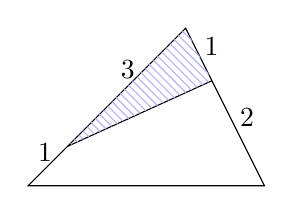
\begin{tikzpicture}[scale=1.0]
    \begin{scope}[shift={(0,0)}]
      \coordinate (A) at (2,2);
      \coordinate (B) at (0,0);
      \coordinate (C) at (3,0);
      \coordinate (D) at ($.75*(B) + .25*(A)$);
      \coordinate (E) at ($2/3*(A) + 1/3*(C)$);
      \draw(E)--(D)
              --(B)node[pos=.15,left]{$1$}
              --(C)
              --(E)node[pos=.65,right]{$2$}
              --(A)node[pos=.65,right]{$1$}
              --(D)node[pos=.35,left]{$3$};
      \fill[pattern=north west lines,pattern color=blue!30](A)--(D)--(E)--cycle;
    \end{scope}
  \end{tikzpicture}
\end{example}
\begin{proof}[解]
  由共角定理,阴影部分与大三角形面积比为
  \begin{align*}
    \frac{3\times 1}{(3+1)\times(1+2)}=\frac{3}{3\times4}=\frac14
  \end{align*}
  从而在大三角形中,阴影部分面积占$\dfrac14$,非阴影部分点$\dfrac34$,阴影与非阴影面积之比为$1:3$。
\end{proof}

\begin{question}
  以下图形的阴影与非阴影面积之间的比例关系同样可应用鸟头定理,请自行思考。

  \centering
  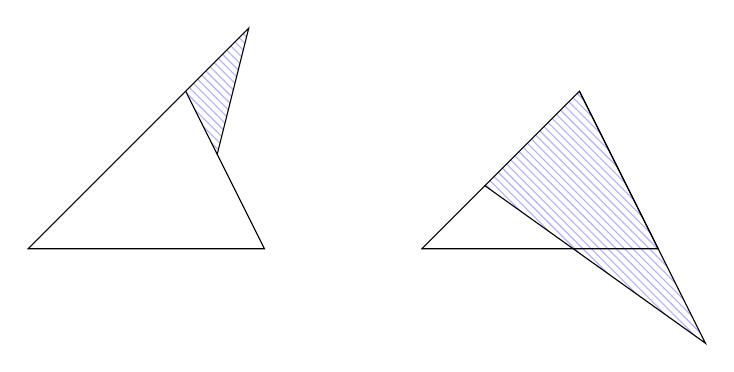
\begin{tikzpicture}[scale=1.0]
    \begin{scope}[shift={(0,0)}]
      \coordinate(A) at (2,2);
      \coordinate(B) at (0,0);
      \coordinate(C) at (3,0);
      \coordinate(D) at ($.4*(C)+.6*(A)$);
      \coordinate(E) at ($1.4*(A)$);
      \draw[pattern=north west lines,pattern color=blue!30](A)--(D)--(E)--cycle;
      \draw(D)--(C)--(B)--(A);
    \end{scope}

    \begin{scope}[shift={(5,0)}]
      \coordinate(A) at (2,2);
      \coordinate(B) at (0,0);
      \coordinate(C) at (3,0);
      \coordinate(D) at ($1.6*(C)-.6*(A)$);
      \coordinate(E) at ($.4*(A)$);
      \draw[pattern=north west lines,pattern color=blue!30](A)--(D)--(E)--cycle;
      \draw(A)--(C)--(B)--(E);
    \end{scope}

    \begin{scope}[shift={(8,0)}]
      
    \end{scope}
  \end{tikzpicture}
\end{question}


\begin{theorem}[蝴蝶定理]
  如图,任意凸四边形的对角线将四边形分成$4$个小三角形,则其面积$S_1,S_2,S_3,S_4$满足以下关系
  \begin{align*}
    S_1S_3=S_2S_4
  \end{align*}

  \centering
  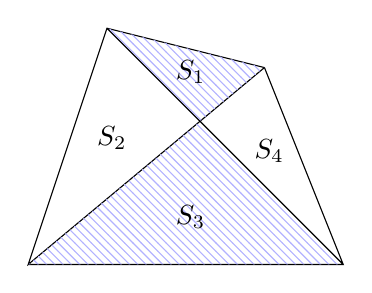
\begin{tikzpicture}[scale=1.0]
    \coordinate(A)at(0,0);
    \coordinate(B)at(4,0);
    \coordinate(C)at(3,2.5);
    \coordinate(D)at(1,3);
    \draw(A)--(B)--(C)--(D)--(A)--(C) (B)--(D);
    \tkzInterLL(A,C)(B,D)\tkzGetPoint{O}
    \fill[pattern=north west lines,pattern color=blue!30](A)--(O)--(B)--cycle;
    \fill[pattern=north west lines,pattern color=blue!30](C)--(O)--(D)--cycle;
    \node at ($1/3*(D)+1/3*(A)+1/3*(O)$) {$S_2$};
    \node at ($1/3*(A)+1/3*(B)+1/3*(O)$) {$S_3$};
    \node at ($1/3*(B)+1/3*(C)+1/3*(O)$) {$S_4$};
    \node at ($1/3*(C)+1/3*(D)+1/3*(O)$) {$S_1$};
  \end{tikzpicture}
\end{theorem}
\begin{proof}
  找同底或等高关系,可得$\dfrac{S_1}{S_2}=\dfrac{S_4}{S_3}$,变换一下即得证。
\end{proof}

\begin{example}[梯形中的蝴蝶定理]
  如图,梯形中的上下底边长分别为$a$和$b$,则对角线分成的$4$个小三角形的面积有如下关系:
  \begin{align*}
    S_1:S_2:S_3:S_4=a^2:ab:b^2:ab
  \end{align*}

  \centering
  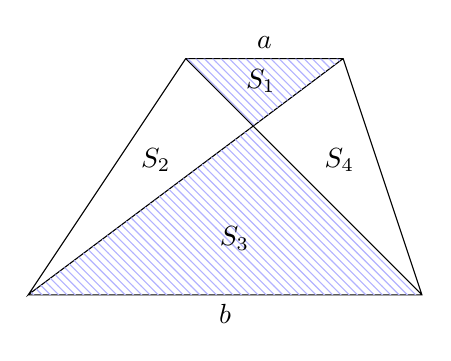
\begin{tikzpicture}[scale=1.0]
    \coordinate(A)at(0,0);
    \coordinate(B)at(5,0);
    \coordinate(C)at(4,3);
    \coordinate(D)at(2,3);
    \draw(A)--(B) node[midway,below]{$b$}--(C)--(D) node[midway,above]{$a$}--(A)--(C) (B)--(D);
    \tkzInterLL(A,C)(B,D)\tkzGetPoint{O}
    \fill[pattern=north west lines,pattern color=blue!30](A)--(O)--(B)--cycle;
    \fill[pattern=north west lines,pattern color=blue!30](C)--(O)--(D)--cycle;
    \node at ($1/3*(D)+1/3*(A)+1/3*(O)$) {$S_2$};
    \node at ($1/3*(A)+1/3*(B)+1/3*(O)$) {$S_3$};
    \node at ($1/3*(B)+1/3*(C)+1/3*(O)$) {$S_4$};
    \node at ($1/3*(C)+1/3*(D)+1/3*(O)$) {$S_1$};
  \end{tikzpicture}
\end{example}
\begin{proof}
  首先由三角形相似性,有$S_1:S_3=a^2:b^2$。其次$S_2+S_3$与$S_4+S_3$同底等高从而面积相等,也就是$S_2=S_4$。再由蝴蝶定理,并令$S_1=a^2$,从而有$S_3=b^2$,并且
  \begin{align*}
    S_1\cdot S_3=S_2\cdot S_4\implies a^2 \cdot b^2 = S_2^2\implies S_2=ab&\qedhere
  \end{align*}
\end{proof}


\begin{theorem}[燕尾定理]
  如图,$D,E,F$分别是三角形$ABC$三边上一点,且$AD$、$BE$与$CF$有共同的交点$O$,则
  \begin{align*}
    S_{\triangle ABO}:S_{\triangle ACO} = S_{\triangle OBD}:S_{\triangle OCD} = BD:CD
  \end{align*}
  其余三角形有类似结论。
  
  \centering
  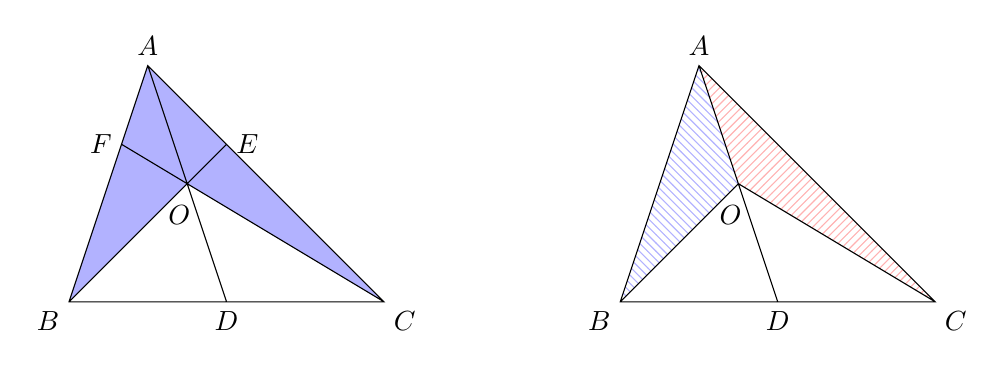
\begin{tikzpicture}[scale=1.0]
    \begin{scope}[shift={(0,0)}]
      \coordinate(A)at(1,3);
      \coordinate(B)at(0,0);
      \coordinate(C)at(4,0);
      \coordinate(O)at(1.5,1.5);
      \tkzInterLL(A,O)(B,C)\tkzGetPoint{D}
      \tkzInterLL(B,O)(C,A)\tkzGetPoint{E}
      \tkzInterLL(C,O)(A,B)\tkzGetPoint{F}
      \fill[color=blue!30](A)--(B)--(O)--(C)--(A);
      \draw(A)--(B)--(C)--cycle (A)--(D) (B)--(E) (C)--(F);
      \tkzLabelPoints[above](A)
      \tkzLabelPoints[below left](B)
      \tkzLabelPoints[below right](C)
      \tkzLabelPoints[below](D)
      \tkzLabelPoints[right](E)
      \tkzLabelPoints[left](F)
      \node at($(O) + (-.1,-.4)$) {$O$};
    \end{scope}

    \begin{scope}[shift={(7,0)}]
      \coordinate(A)at(1,3);
      \coordinate(B)at(0,0);
      \coordinate(C)at(4,0);
      \coordinate(O)at(1.5,1.5);
      \tkzInterLL(A,O)(B,C)\tkzGetPoint{D}
      \tkzInterLL(B,O)(C,A)\tkzGetPoint{E}
      \tkzInterLL(C,O)(A,B)\tkzGetPoint{F}
      \fill[pattern=north west lines,pattern color=blue!30](A)--(B)--(O);
      \fill[pattern=north east lines,pattern color=red!30](A)--(C)--(O);
      \draw(A)--(B)--(C)--cycle (A)--(D) (B)--(O) (C)--(O);
      \tkzLabelPoints[above](A)
      \tkzLabelPoints[below left](B)
      \tkzLabelPoints[below right](C)
      \tkzLabelPoints[below](D)
      % \tkzLabelPoints[right](E)
      % \tkzLabelPoints[left](F)
      \node at($(O) + (-.1,-.4)$) {$O$};
    \end{scope}
  \end{tikzpicture}
\end{theorem}
\begin{proof}[说明]
  如第二图的最小模型,若只考虑一个燕尾,可在$AD$上随意取点$O$即有上述结论,即无需知道$E,F$两点。
\end{proof}

\begin{example}
  在燕尾定理的图中,证明
  \begin{align*}
    \frac{BD}{DC}\times\frac{CE}{EA}\times\frac{AF}{FB}=1
  \end{align*}
\end{example}
\begin{proof}
  由燕尾定理,有
  \begin{align*}
    S_{\triangle ABO}:S_{\triangle ACO} &= BD:DC\\
    S_{\triangle ACO}:S_{\triangle CBO} &= AF:FB\\
    S_{\triangle CBO}:S_{\triangle ABO} &= CE:EA
  \end{align*}
  三式相乘可得。
\end{proof}

\chapter{圆}
\label{chap:circle}

到一点的距离是某个固定常数(即半径)的点的集合,在三维空间中就是球面,而在平面中就是圆。圆在生活中应用非常广泛,比如下水道井盖为什么是圆的,其中一个原因就是不管井盖怎么放都不会掉到井里去。

\section{圆与三角形}
\label{sec:circle-and-triangle}

\begin{example}
  以固定长度$a$为斜边作一个直角三角形,则这些三角形中,该斜边上的高的最大值是多少?
\end{example}
\begin{proof}[提示]\mbox{}\par
  \begin{center}
    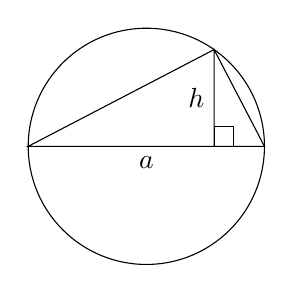
\begin{tikzpicture}[scale=1.0]
      \foreach \r/\theta in{1.5/55}{
        \draw(0,0)circle(1.5);
        \coordinate(A)at(-1.5,0);\coordinate(B)at(1.5,0);\coordinate(C)at(\theta:1.5);
        \coordinate(D)at($(B)!(C)!(A)$);
        \draw(C)--(A)--(B)node[midway,below]{$a$}--(C)--(D)  node[midway, left]{$h$};
        \tkzMarkRightAngle(C,D,B)
      }
    \end{tikzpicture}
  \end{center}
  另外一个顶点都是落在图中的圆上,显然高的最大值是圆的半径。
\end{proof}

\begin{theorem}[圆内接四边形]
  平面上四边形$ABCD$,以下几个命题等价:
  \begin{enumerate}
  \item $A,B,C,D$共圆;
  \item $\angle A + \angle C = \pi$;
  \item $\angle ACB = \angle ADB$。
  \end{enumerate}
\end{theorem}
\begin{proof}[提示]
  $(1)\implies(2)$及$(1)\implies(3)$都是显然的。

  $(2)\implies(1)$。等价于固定$A,B,C$,平面上不含点$B$的直线$AC$的另一侧上所有使$\angle AD'C + \angle ABC=\pi$的动点$D'$都落在$\triangle ABC$的外接圆上。分动点在圆内及圆外两种情况考虑即可。

  \begin{center}
    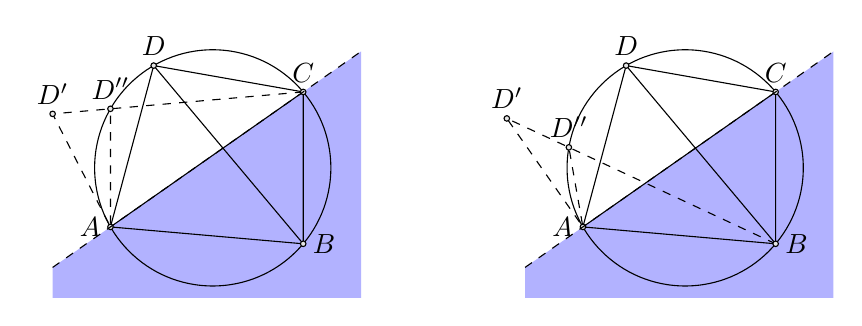
\begin{tikzpicture}[scale=1.0]
      \begin{scope}
        \foreach \r/\a/\b/\c/\d/\dd in{1.5/210/320/40/120/150}{
          \coordinate(O)at(0,0);
          \coordinate[label=left:$A$](A)at(\a:\r);
          \coordinate[label=above:$C$](C)at(\c:\r);
          \coordinate[label=above:$D$](D)at(\d:\r);
          \coordinate[label=above:$D''$](D'')at(\dd:\r);
          % \tkzInterLC(C,D')(O,C)\tkzGetPoints{D''}{}
          \coordinate[label=above:$D'$](D')at($(D'')+.3*(D'')-.3*(C)$);
          \coordinate(A')at($(A)+.3*(A)-.3*(C)$);
          \coordinate(C')at($(C)+.3*(C)-.3*(A)$);
          \coordinate(X)at(0,-1.1*\r);
          \fill[color=blue!30](A')--(A' |- X)--(C' |- X)--(C');
          \coordinate[label=right:$B$](B)at(\b:\r);
          \draw(0,0)circle(\r);
          \draw(A)--(B)--(C)--(D)--cycle (A)--(C) (B)--(D);
          \draw[dashed](C)--(D')--(A)--(D'');
          \tkzDrawPoints(A,B,C,D,D',D'')
          \draw[dashed](A')--(C');
        }
      \end{scope}
      \begin{scope}[shift={(6,0)}]
        \foreach \r/\a/\b/\c/\d/\dd in{1.5/210/320/40/120/170}{
          \coordinate(O)at(0,0);
          \coordinate[label=left:$A$](A)at(\a:\r);
          \coordinate[label=above:$C$](C)at(\c:\r);
          \coordinate(A')at($(A)+.3*(A)-.3*(C)$);
          \coordinate(C')at($(C)+.3*(C)-.3*(A)$);
          \fill[color=blue!30](A')--(A' |- X)--(C' |- X)--(C');

          \coordinate[label=above:$D$](D)at(\d:\r);
          \coordinate[label=above:$D''$](D'')at(\dd:\r);
          \coordinate[label=right:$B$](B)at(\b:\r);
          \coordinate[label=above:$D'$](D')at($(D'')+.3*(D'')-.3*(B)$);
          \coordinate(X)at(0,-1.1*\r);
          \draw(0,0)circle(\r);
          \draw(A)--(B)--(C)--(D)--cycle (A)--(C) (B)--(D);
          \draw[dashed](B)--(D')--(A)--(D'');
          \tkzDrawPoints(A,B,C,D,D',D'')
          \draw[dashed](A')--(C');
        }
      \end{scope}
    \end{tikzpicture}
  \end{center}

  $(3)\implies(1)$。类似的,分半平面内圆内与圆外两种情况分别考虑动点$D'$,若$\angle AD'B=\angle ACB$,则$D'$必落在$\triangle ABC$的外接圆上\footnote{但外接圆上的任一点$P$不一定有$\angle APB=\angle ACB$,除非$A,B$是圆上一直径的两端点。},这可以分动点在圆内及圆外两种情况分别考虑得到。
\end{proof}

\begin{theorem}[割线定理]
  平面上线段$AB$与$CD$相交于$E$,则以下命题等价:
  \begin{enumerate}
  \item $A,B,C,D$共圆;
  \item $AE\cdot EB=CE\cdot ED$。
  \end{enumerate}
\end{theorem}
\begin{proof}[提示]
  $(1)\implies(2)$。连接$AC$及$BD$(或者连接$AD$及$BC$),由三角形相似显然可得。

  \begin{center}
    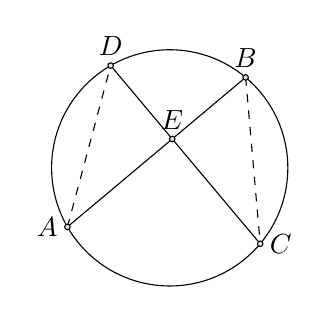
\begin{tikzpicture}
      \foreach \r/\a/\b/\c/\d in{1.5/210/50/320/120}{
        \coordinate(O)at(0,0);
        \coordinate[label=left:$A$](A)at(\a:\r);
        \coordinate[label=above:$B$](B)at(\b:\r);
        \coordinate[label=right:$C$](C)at(\c:\r);
        \coordinate[label=above:$D$](D)at(\d:\r);
        \tkzInterLL(A,B)(C,D)\tkzGetPoint{E}
        \draw(O)circle(\r);
        \draw(A)--(B) (C)--(D);
        \draw[dashed](A)--(D) (B)--(C);
        \tkzDrawPoints(A,B,C,D,E)
        \node[above]at(E){$E$};
      }
    \end{tikzpicture}
  \end{center}

  $(2)\implies(1)$。由$AE\cdot EB=CE\cdot ED$,可知$\triangle AED\sim\triangle CEB$,从而$\angle A=\angle C$,四点共圆。
\end{proof}

\chapter{几何}
\label{chap:geometry}

\begin{example}
  有6个棱长是$3\times4\times5$的相同长方体。现在要把它们的一些面染成红色,要求其中一个染一面,一个染两面,一个染三面,一个染四面,一个染五面,一个染六面。染完后将6个长方体都切成$1\times1\times1$的正方体,问如何染色才能使切出来的正方体中只有一面是红色的个数最多?
\end{example}
\begin{proof}[提示]
  6个正方体分别考虑,使其染完后切成的正方体中含单面红色的最多。
  \begin{enumerate}
  \item 染6面红色的长方体,只有一个染色方案,其中切完后,只有一面是红色的小正方体共有$(2+3+6)\times2=22$个(阴影部分)。

    \begin{center}
      % \tdplotsetmaincoords{70}{120}
      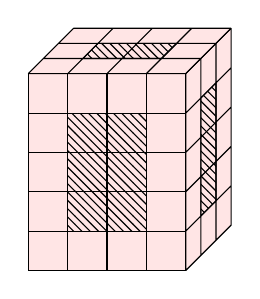
\begin{tikzpicture}[scale=.5,
        % tdplot_main_coords,
        fill red/.style={fill=red, fill opacity=.1},
        slash lines/.style={pattern=north west lines, pattern color=black}]
        \fill[canvas is yz plane at x=4,fill red   ](0,0)rectangle(5,3);
        \draw[canvas is yz plane at x=4,slash lines](1,1)rectangle(4,2);
        \draw[canvas is yz plane at x=4            ](0,0)grid     (5,3);

        \fill[canvas is xz plane at y=5,fill red   ](0,0)rectangle(4,3);
        \draw[canvas is xz plane at y=5,slash lines](1,1)rectangle(3,2);
        \draw[canvas is xz plane at y=5            ](0,0)grid     (4,3);

        \fill[canvas is xy plane at z=3,fill red   ](0,0)rectangle(4,5);
        \draw[canvas is xy plane at z=3,slash lines](1,1)rectangle(3,4);
        \draw[canvas is xy plane at z=3            ](0,0)grid     (4,5);
      \end{tikzpicture}
    \end{center}
    
  \item 只染一个面时,如下图有三种染法。其中第三种染法使得切成小正方体后只有一面是红色的小正方体的数量最多,为$4\times5=20$个。

    \begin{center}
      % \tdplotsetmaincoords{70}{120}
      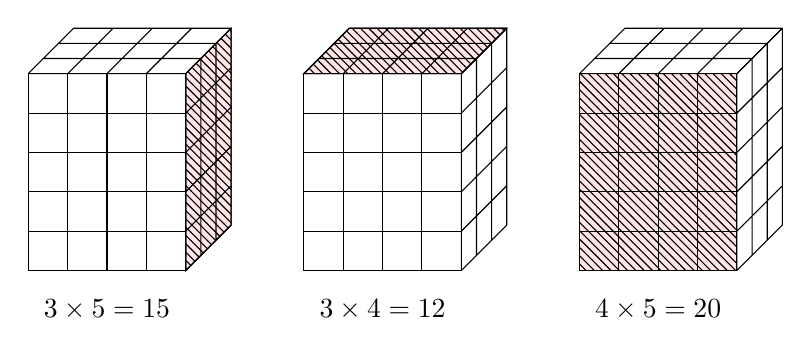
\begin{tikzpicture}[scale=.5,
        % tdplot_main_coords,
        fill red/.style={fill=red, fill opacity=.1},
        slash lines/.style={pattern=north west lines, pattern color=black}]
        \begin{scope}[shift={(0,0)}]
          \fill[canvas is yz plane at x=4,fill red   ](0,0)rectangle(5,3);
          \draw[canvas is yz plane at x=4,slash lines](0,0)rectangle(5,3);
          \draw[canvas is yz plane at x=4            ](0,0)grid     (5,3);

          % \fill[canvas is xz plane at y=5,fill red   ](0,0)rectangle(4,3);
          % \draw[canvas is xz plane at y=5,slash lines](1,1)rectangle(3,2);
          \draw[canvas is xz plane at y=5            ](0,0)grid     (4,3);

          % \fill[canvas is xy plane at z=3,fill red   ](0,0)rectangle(4,5);
          % \draw[canvas is xy plane at z=3,slash lines](1,1)rectangle(3,4);
          \draw[canvas is xy plane at z=3            ](0,0)grid     (4,5) node at(2,-1){$3\times5=15$};
        \end{scope}

        \begin{scope}[shift={(7,0)}]
          % \fill[canvas is yz plane at x=4,fill red   ](0,0)rectangle(5,3);
          % \draw[canvas is yz plane at x=4,slash lines](1,1)rectangle(4,2);
          \draw[canvas is yz plane at x=4            ](0,0)grid     (5,3);

          \fill[canvas is xz plane at y=5,fill red   ](0,0)rectangle(4,3);
          \draw[canvas is xz plane at y=5,slash lines](0,0)rectangle(4,3);
          \draw[canvas is xz plane at y=5            ](0,0)grid     (4,3);

          % \fill[canvas is xy plane at z=3,fill red   ](0,0)rectangle(4,5);
          % \draw[canvas is xy plane at z=3,slash lines](1,1)rectangle(3,4);
          \draw[canvas is xy plane at z=3            ](0,0)grid     (4,5) node at(2,-1){$3\times4=12$};
        \end{scope}

        \begin{scope}[shift={(14,0)}]
          % \fill[canvas is yz plane at x=4,fill red   ](0,0)rectangle(5,3);
          % \draw[canvas is yz plane at x=4,slash lines](1,1)rectangle(4,2);
          \draw[canvas is yz plane at x=4            ](0,0)grid     (5,3);

          % \fill[canvas is xz plane at y=5,fill red   ](0,0)rectangle(4,3);
          % \draw[canvas is xz plane at y=5,slash lines](1,1)rectangle(3,2);
          \draw[canvas is xz plane at y=5            ](0,0)grid     (4,3);

          \fill[canvas is xy plane at z=3,fill red   ](0,0)rectangle(4,5);
          \draw[canvas is xy plane at z=3,slash lines](0,0)rectangle(4,5);
          \draw[canvas is xy plane at z=3            ](0,0)grid     (4,5) node at(2,-1){$4\times5=20$};
        \end{scope}
      \end{tikzpicture}
    \end{center}


  \item 只染两个面时,有如下图三种相邻的染法。其中第三种染法使得切成小正方体后只有一面是红色的小正方体的数量最多,为$5\times\left((4-1)+(3-1)\right)=25$个。

    \begin{center}
      % \tdplotsetmaincoords{70}{120}
      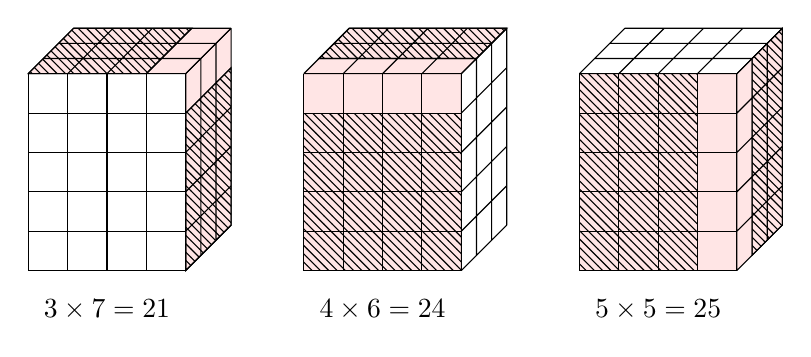
\begin{tikzpicture}[scale=.5,
        % tdplot_main_coords,
        fill red/.style={fill=red, fill opacity=.1},
        slash lines/.style={pattern=north west lines, pattern color=black}]
        \begin{scope}[shift={(0,0)}]
          \fill[canvas is yz plane at x=4,fill red   ](0,0)rectangle(5,3);
          \draw[canvas is yz plane at x=4,slash lines](0,0)rectangle(4,3);
          \draw[canvas is yz plane at x=4            ](0,0)grid     (5,3);

          \fill[canvas is xz plane at y=5,fill red   ](0,0)rectangle(4,3);
          \draw[canvas is xz plane at y=5,slash lines](0,0)rectangle(3,3);
          \draw[canvas is xz plane at y=5            ](0,0)grid     (4,3);

          % \fill[canvas is xy plane at z=3,fill red   ](0,0)rectangle(4,5);
          % \draw[canvas is xy plane at z=3,slash lines](1,1)rectangle(3,4);
          \draw[canvas is xy plane at z=3            ](0,0)grid     (4,5) node at(2,-1){$3\times7=21$};
        \end{scope}

        \begin{scope}[shift={(7,0)}]
          % \fill[canvas is yz plane at x=4,fill red   ](0,0)rectangle(5,3);
          % \draw[canvas is yz plane at x=4,slash lines](1,1)rectangle(4,2);
          \draw[canvas is yz plane at x=4            ](0,0)grid     (5,3);

          \fill[canvas is xz plane at y=5,fill red   ](0,0)rectangle(4,3);
          \draw[canvas is xz plane at y=5,slash lines](0,0)rectangle(4,2);
          \draw[canvas is xz plane at y=5            ](0,0)grid     (4,3);

          \fill[canvas is xy plane at z=3,fill red   ](0,0)rectangle(4,5);
          \draw[canvas is xy plane at z=3,slash lines](0,0)rectangle(4,4);
          \draw[canvas is xy plane at z=3            ](0,0)grid     (4,5) node at(2,-1){$4\times6=24$};;
        \end{scope}

        \begin{scope}[shift={(14,0)}]
          \fill[canvas is yz plane at x=4,fill red   ](0,0)rectangle(5,3);
          \draw[canvas is yz plane at x=4,slash lines](0,0)rectangle(5,2);
          \draw[canvas is yz plane at x=4            ](0,0)grid     (5,3);

          % \fill[canvas is xz plane at y=5,fill red   ](0,0)rectangle(4,3);
          % \draw[canvas is xz plane at y=5,slash lines](1,1)rectangle(3,2);
          \draw[canvas is xz plane at y=5            ](0,0)grid     (4,3);

          \fill[canvas is xy plane at z=3,fill red   ](0,0)rectangle(4,5);
          \draw[canvas is xy plane at z=3,slash lines](0,0)rectangle(3,5);
          \draw[canvas is xy plane at z=3            ](0,0)grid     (4,5) node at(2,-1){$5\times5=25$};;
        \end{scope}
      \end{tikzpicture}
    \end{center}

    还有三种不相邻的染法。由只染一面的结论可知,染两面$5\times4$的两个不相邻面时,切成的小方块只有一面是红色的数量最多,为$5\times4\times2=40$个。

    \begin{center}
      % \tdplotsetmaincoords{70}{120}
      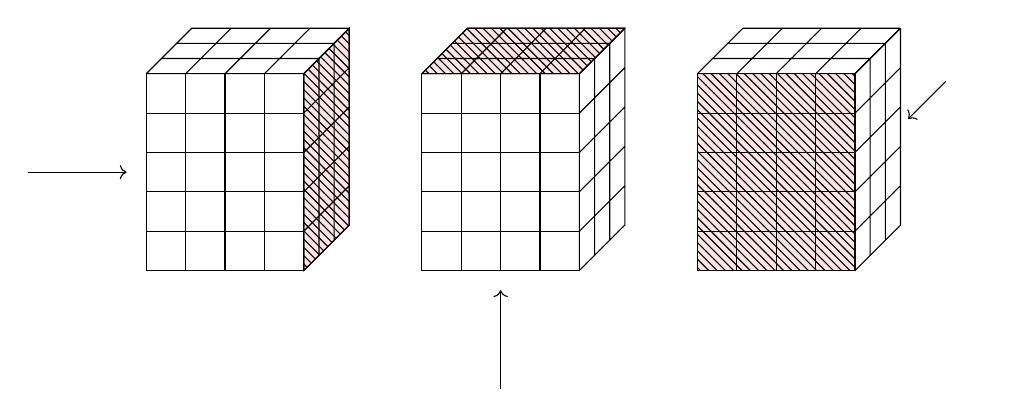
\begin{tikzpicture}[scale=.5,
        % tdplot_main_coords,
        fill red/.style={fill=red, fill opacity=.1},
        slash lines/.style={pattern=north west lines, pattern color=black}]
        \begin{scope}[shift={(0,0)}]
          \fill[canvas is yz plane at x=4,fill red   ](0,0)rectangle(5,3);
          \draw[canvas is yz plane at x=4,slash lines](0,0)rectangle(5,3);
          \draw[canvas is yz plane at x=4            ](0,0)grid     (5,3);
          \draw[canvas is xy plane at z=3,->](-3,2.5)--(-.5,2.5) node[midway,above]{左边};

          % \fill[canvas is xz plane at y=5,fill red   ](0,0)rectangle(4,3);
          % \draw[canvas is xz plane at y=5,slash lines](1,1)rectangle(3,2);
          \draw[canvas is xz plane at y=5            ](0,0)grid     (4,3);

          % \fill[canvas is xy plane at z=3,fill red   ](0,0)rectangle(4,5);
          % \draw[canvas is xy plane at z=3,slash lines](1,1)rectangle(3,4);
          \draw[canvas is xy plane at z=3            ](0,0)grid     (4,5);
        \end{scope}

        \begin{scope}[shift={(7,0)}]
          % \fill[canvas is yz plane at x=4,fill red   ](0,0)rectangle(5,3);
          % \draw[canvas is yz plane at x=4,slash lines](1,1)rectangle(4,2);
          \draw[canvas is yz plane at x=4            ](0,0)grid     (5,3);

          \fill[canvas is xz plane at y=5,fill red   ](0,0)rectangle(4,3);
          \draw[canvas is xz plane at y=5,slash lines](0,0)rectangle(4,3);
          \draw[canvas is xz plane at y=5            ](0,0)grid     (4,3);
          \draw[canvas is xy plane at z=3,->](2,-3)--(2,-.5) node[midway,right]{底面};

          % \fill[canvas is xy plane at z=3,fill red   ](0,0)rectangle(4,5);
          % \draw[canvas is xy plane at z=3,slash lines](1,1)rectangle(3,4);
          \draw[canvas is xy plane at z=3            ](0,0)grid     (4,5);
        \end{scope}

        \begin{scope}[shift={(14,0)}]
          % \fill[canvas is yz plane at x=4,fill red   ](0,0)rectangle(5,3);
          % \draw[canvas is yz plane at x=4,slash lines](1,1)rectangle(4,2);
          \draw[canvas is yz plane at x=4            ](0,0)grid     (5,3);

          % \fill[canvas is xz plane at y=5,fill red   ](0,0)rectangle(4,3);
          % \draw[canvas is xz plane at y=5,slash lines](1,1)rectangle(3,2);
          \draw[canvas is xz plane at y=5            ](0,0)grid     (4,3);

          \fill[canvas is xy plane at z=3,fill red   ](0,0)rectangle(4,5);
          \draw[canvas is xy plane at z=3,slash lines](0,0)rectangle(4,5);
          \draw[canvas is xy plane at z=3            ](0,0)grid     (4,5);
          \draw[canvas is yz plane at x=4,->](2.5,-3)--(2.5,-.5)node[pos=0,right]{背面};
        \end{scope}
      \end{tikzpicture}
    \end{center}
    
  \item 染五面红色只有三种染法(相当于取哪一面不染,与染一面的类似)。

    \begin{center}
      % \tdplotsetmaincoords{70}{120}
      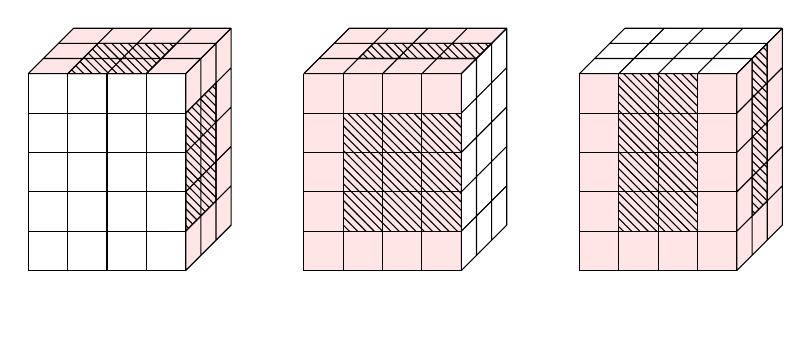
\begin{tikzpicture}[scale=.5,
        % tdplot_main_coords,
        fill red/.style={fill=red, fill opacity=.1},
        slash lines/.style={pattern=north west lines, pattern color=black}]
        \begin{scope}[shift={(0,0)}]
          \fill[canvas is yz plane at x=4,fill red   ](0,0)rectangle(5,3);
          \draw[canvas is yz plane at x=4,slash lines](1,1)rectangle(4,3);
          \draw[canvas is yz plane at x=4            ](0,0)grid     (5,3);

          \fill[canvas is xz plane at y=5,fill red   ](0,0)rectangle(4,3);
          \draw[canvas is xz plane at y=5,slash lines](1,1)rectangle(3,3);
          \draw[canvas is xz plane at y=5            ](0,0)grid     (4,3);

          % \fill[canvas is xy plane at z=3,fill red   ](0,0)rectangle(4,5);
          % \draw[canvas is xy plane at z=3,slash lines](1,1)rectangle(3,4);
          \draw[canvas is xy plane at z=3            ](0,0)grid     (4,5) node at(2,-1){只有前面不染};
        \end{scope}

        \begin{scope}[shift={(7,0)}]
          % \fill[canvas is yz plane at x=4,fill red   ](0,0)rectangle(5,3);
          % \draw[canvas is yz plane at x=4,slash lines](1,1)rectangle(4,2);
          \draw[canvas is yz plane at x=4            ](0,0)grid     (5,3);

          \fill[canvas is xz plane at y=5,fill red   ](0,0)rectangle(4,3);
          \draw[canvas is xz plane at y=5,slash lines](1,1)rectangle(4,2);
          \draw[canvas is xz plane at y=5            ](0,0)grid     (4,3);

          \fill[canvas is xy plane at z=3,fill red   ](0,0)rectangle(4,5);
          \draw[canvas is xy plane at z=3,slash lines](1,1)rectangle(4,4);
          \draw[canvas is xy plane at z=3            ](0,0)grid     (4,5) node at(2,-1){只有右面不染};;
        \end{scope}

        \begin{scope}[shift={(14,0)}]
          \fill[canvas is yz plane at x=4,fill red   ](0,0)rectangle(5,3);
          \draw[canvas is yz plane at x=4,slash lines](1,1)rectangle(5,2);
          \draw[canvas is yz plane at x=4            ](0,0)grid     (5,3);

          % \fill[canvas is xz plane at y=5,fill red   ](0,0)rectangle(4,3);
          % \draw[canvas is xz plane at y=5,slash lines](1,1)rectangle(3,2);
          \draw[canvas is xz plane at y=5            ](0,0)grid     (4,3);

          \fill[canvas is xy plane at z=3,fill red   ](0,0)rectangle(4,5);
          \draw[canvas is xy plane at z=3,slash lines](1,1)rectangle(3,5);
          \draw[canvas is xy plane at z=3            ](0,0)grid     (4,5) node at(2,-1){只有上面不染};;
        \end{scope}
      \end{tikzpicture}
    \end{center}

    第一种,$4\times2(\text{上面加下面})+6\times2(\text{左面加右面})+6(\text{背面})=26$。

    第二种,$3\times2(\text{上面加下面})+9\times2(\text{前面加后面})+3(\text{左面})=27$。

    第三种,$8\times2(\text{前面加后面})+4\times2(\text{左面加右面})+2(\text{底面})=26$。

  \item 染四面红色只有六种染法(相当于取哪两面不染,与染两面的类似)。
  \item 染三面红色时最麻烦,染色方案最多。请自行考虑。
  \end{enumerate}

  六个长方体都讨论完,结论自然就出来了。
\end{proof}

\section{尺规作图}
\label{sec:draw-with-ruler}

\begin{example}
  只用圆规找到给圆的半径。
\end{example}

\begin{example}[上海,1956]
  给定圆周,只用圆规将圆周四等分。
\end{example}

\chapter{几何不等式}
\label{chap:geometric-inequality}

\begin{theorem}[Pythagorean不等式]
  记三角形的三边分别为$a\le b\le c$,则
  \begin{enumerate}
  \item 三角形是直角三角形$\iff a^2+b^2=c^2$;
  \item 三角形是锐角三角形$\iff a^2+b^2>c^2$;
  \item 三角形是钝角三角形$\iff a^2+b^2<c^2$。
  \end{enumerate}
\end{theorem}

\begin{theorem}[等周不等式,Isoperimetric Inequality]
  若一个平面图形的面积与周长分别为$A$和$P$,则$4\pi A\le P^2$。也就是说在平面上用长度为$P$的线段能围成的最大面积是半径为$\dfrac{P}{2\pi}$的圆,其面积为$\dfrac{P^2}{4\pi}$。
\end{theorem}

\begin{theorem}[三角不等式,Trigonometric Inequality]
  记三角形的三个角分别为$A,B,C$,则
  \begin{align*}
    \sin A +\sin B + \sin C&\le\frac{3\sqrt3}{2}\\
    \cos A +\cos B + \cos C&\le\phantom{3}\,\frac{3}{2}
  \end{align*}
\end{theorem}
\begin{proof}
  由$\sin(x)$及$\cos(x)$在$[0,\pi]$上是凹函数,利用Jensen不等式可得。
\end{proof}

\begin{theorem}[相交弦定理,Intersecting Chords Theorem]
  圆内的两条相交弦,被交点分成的两条线段长的积相等。
\end{theorem}
\begin{proof}
  利用相似三角形可得。
\end{proof}

\begin{theorem}[海伦公式,海伦-秦九韶公式,Heron's Formula]
  记三角形的三边边长分别为$a,b,c$,其半周长$s=\dfrac{a+b+c}2$,则三角形的面积为
  \begin{align}
    S=\sqrt{s(s-a)(s-b)(s-c)}
  \end{align}
\end{theorem}
\begin{proof}
  用余弦公式可证。或者用勾股定理证明$c$边对应的高
  \begin{align*}
    h=\frac{4s(s-a)(s-b)(s-c)}{c^2} &\qedhere
  \end{align*}
\end{proof}

\begin{theorem}
  如图~\ref{fig:r-of-incircle}所示,三角形内切圆将各边分别分割成$x,y,z$的长度,则可得到内切圆的半径公式
  \begin{align}
    r=\sqrt{\frac{xyz}{x+y+z}}=\frac{S}{s}
  \end{align}
\end{theorem}
\begin{figure}[htbp]
  \centering
  \begin{tikzpicture}[scale=1]
    \tkzDefPoint[label=below left:$A$](0,0){A}
    \tkzDefPoint[label=below right:$B$](6,0){B}
    \tkzDefPoint[label=above:$C$](5,5){C}
    
    \tkzDefCircle[in](A,B,C)\tkzGetPoint{I}\tkzGetLength{rIN}
    \tkzDrawCircle[R](I,\rIN pt);
    \tkzDrawSegments(A,B B,C C,A)
    % \tkzDrawSegments[dashed](I,A I,B I,C)

    \coordinate(IA) at ($(B)!(I)!(C)$);
    \coordinate(IB) at ($(C)!(I)!(A)$);
    \coordinate(IC) at ($(A)!(I)!(B)$);

    %\tkzDrawSegments[dashed](I,IA I,IB I,IC)
    \tkzMarkRightAngle[color=blue](B,IC,I)
    \tkzMarkRightAngle[color=blue](C,IA,I)
    \tkzMarkRightAngle[color=blue](A,IB,I)

    \foreach \p in{A,B,C,I,IA,IB,IC}{
      \tkzDrawPoint(\p)
    }
    \tkzLabelPoints[below left](I)

    \draw(A)--(IC) node[below,sloped,midway]{$x$};
    \draw(A)--(IB) node[above left,sloped,midway]{$x$};
    \draw(B)--(IC) node[below,sloped,midway]{$y$};
    \draw(B)--(IA) node[above right,sloped,midway]{$y$};
    \draw(C)--(IB) node[above left,sloped,midway]{$z$};
    \draw(C)--(IA) node[above right,sloped,midway]{$z$};
    \draw[dashed](I)--(IC);
    \draw[dashed](I)--(IA) node[above,sloped,midway]{$r$};
    \draw[dashed](I)--(IB);% node[below left,sloped,midway]{$r$};
  \end{tikzpicture}
  \caption{三角形内切圆的半径}
  \label{fig:r-of-incircle}
\end{figure}
\begin{proof}
  令$s=\dfrac{a+b+c}2$是半周长,则显然有$x=s-a, y=s-b, z=s-c$。由海伦公式可得
  \begin{align*}
    S=\sqrt{xyz(x+y+z)}
  \end{align*}
  另一方面,$S=\dfrac12r(a+b+c)=r(x+y+z)$,从而可得。
\end{proof}

\begin{theorem}[Euler定理]
  记$R,r$分别是三角形的外接圆和内切圆半径,$d$是外接圆与内切圆圆心间的距离,则$d^2=R(R-2r)$,或等价的
  \begin{align*}
    \frac1{R-d}+\frac1{R+d}=\frac1r
  \end{align*}
\end{theorem}
\begin{proof}
  记$G,I$分别是外接圆和内切圆的圆心,在过$G$和$I$的直线上找到长度分别为$R+d$和$R-d$的线段,比如直线$GI$与外接圆的交点$P$、$Q$,则线段$IP$和$IQ$分别为$R\pm d$。

  如图\ref{fig:in/circumcircle},延长$CI$得$L$,延长$LG$得$M$,延长$GI$得$P$和$Q$,则$\triangle CID\sim\triangle MLA$,且$LA=LI$,从而
  \begin{align*}
    (R+d)(R-d)&=IP\cdot IQ=IC\cdot IL=IC\cdot LA=ID\cdot LM=2Rr&\qedhere
  \end{align*}
\end{proof}

\begin{figure}[htbp]
  \centering
%\fbox{%Use \fbox to check the boundary of the tikz picture
  \begin{tikzpicture}[scale=1]
    \tkzDefPoint[label=below left:$A$](0,0){A}
    \tkzDefPoint[label=below right:$B$](6,0){B}
    \tkzDefPoint[label=above:$C$](5,5){C}
    
    \tkzDefCircle[in](A,B,C)\tkzGetPoint{I}\tkzGetLength{rIN}
    \tkzDrawCircle[R](I,\rIN pt);
    \tkzDrawSegments(A,B B,C C,A)
    % \tkzDrawSegments[dashed](I,A I,B I,C)

    % \coordinate(IA) at ($(B)!(I)!(C)$);
    \coordinate[label=above left:$D$](IB) at ($(C)!(I)!(A)$);
    % \coordinate(IC) at ($(A)!(I)!(B)$);

    % \tkzDrawSegments[dashed](I,IA I,IB I,IC)
    \tkzDrawSegments[dashed](I,IB)
    % \tkzMarkRightAngle[color=blue](B,IC,I)
    % \tkzMarkRightAngle[color=blue](C,IA,I)
    \tkzMarkRightAngle[color=blue](A,IB,I)

    % circumcircle
    \tkzCircumCenter(A,B,C)\tkzGetPoint{G}
    \tkzDrawCircle(G,A)
    \tkzInterLC(G,I)(G,A)\tkzGetPoints{P}{Q}

    \draw[dashed](A)--(I);
    \draw[dashed](I)--(P);
    \draw[dashed](I)--(Q);
    \draw[thick](G)--(I);

    \tkzInterLC(C,I)(G,A)\tkzGetPoints{}{L}
    \tkzInterLC(L,G)(G,A)\tkzGetPoints{}{M}

    \tkzLabelPoints[left](P)
    \tkzLabelPoints[right](Q,I)
    \tkzLabelPoints[below](L)
    \tkzLabelPoints[below left](G)
    \tkzLabelPoints[above](M)

    \draw[dashed](C)--(L)--(M)--(A)--(L);

    \foreach \p in{A,B,C,I,G,P,Q,IB,L,M}{
      \tkzDrawPoint(\p)
    }

    % emphasize similar triangles
    \draw[very thick](C)--(I)--(IB)--cycle;
    \draw[very thick](M)--(A)--(L)--cycle;
  \end{tikzpicture}
%}
  % Maybe due to BUG of pgfplots, there're wide space between figure
  % and caption, -3cm is measured by eye
  \vspace*{-3cm}
  \caption{三角形的外接圆与内切圆}
  \label{fig:in/circumcircle}
\end{figure}


\begin{theorem}[Euler不等式]
  记$R,r$分别是三角形$\triangle ABC$的外接圆和内切圆半径,则有$R\ge2r$。
\end{theorem}
\begin{proof}
  由Euler定理立得。
\end{proof}

\begin{theorem}\label{th:R-of-circumcircle}
  任意$\triangle ABC$,其三边边长分别为$a,b,c$,面积为$S$,则其外接圆半径为
  \begin{align}
    R=\frac{abc}{4S}
  \end{align}
\end{theorem}
\begin{figure}[htbp]
  \centering
  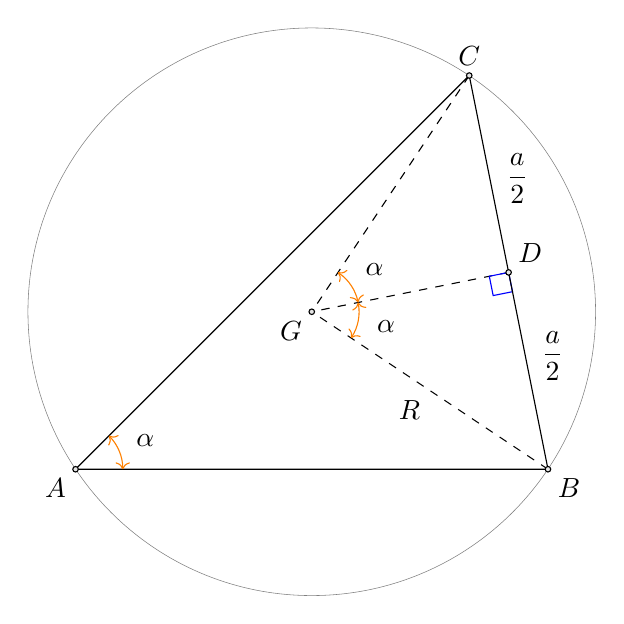
\begin{tikzpicture}[scale=1]
    \tkzDefPoint[label=below left:$A$](0,0){A}
    \tkzDefPoint[label=below right:$B$](6,0){B}
    \tkzDefPoint[label=above:$C$](5,5){C}
    
    % circumcircle
    \tkzCircumCenter(A,B,C)\tkzGetPoint{G}
    \tkzDrawCircle(G,A)
    \tkzLabelPoints[below left](G)

    \coordinate[label=above right:$D$](D) at ($(B)!(G)!(C)$);

    \draw[dashed](B)--(G) node[midway,below left]{$R$};
    \draw[dashed](C)--(G);
    \draw[dashed](D)--(G);
    \tkzMarkRightAngle[color=blue](G,D,B)
    \draw(A)--(B)--(C)
        node[pos=0.20,above right]{$\dfrac{a}2$} 
        node[pos=0.65,above right]{$\dfrac{a}2$} --cycle;

    \draw pic["$\alpha$",draw=orange,<->,angle eccentricity=1.6,angle radius=.6cm] {angle=B--A--C};
    \draw pic["$\alpha$",draw=orange,<->,angle eccentricity=1.6,angle radius=.6cm] {angle=B--G--D};
    \draw pic["$\alpha$",draw=orange,<->,angle eccentricity=1.6,angle radius=.6cm] {angle=D--G--C};

    \foreach \p in{A,B,C,D,G}{
      \tkzDrawPoint(\p)
    }
  \end{tikzpicture}    
  % Maybe due to BUG of pgfplots, there're wide space between figure
  % and caption, -3cm is measured by eye
  \vspace*{-3.5cm}
  \caption{三角形外接圆半径}
  \label{fig:R-of-circumcircle}
\end{figure}
\begin{proof}
  由图~\ref{fig:R-of-circumcircle}容易看出$\angle BAC = \angle CGD = \angle BGD$,从而有
  \begin{align*}
    S_{\triangle ABC} = \frac12 bc\cdot\sin\angle BAC
    = \frac12 bc \cdot \frac{a/2}{R} = \frac{abc}{4R}
  \end{align*}
  从而可算出$R$。
\end{proof}


\begin{theorem}
  任意$\triangle ABC$,记$a,b,c$是其三边边长,$r,R$分别是其内切圆与外接圆半径,则
  \begin{align}
    rR=\frac{abc}{2(a+b+c)}
  \end{align}
\end{theorem}
\begin{proof}
  在定理~\ref{th:R-of-circumcircle},将$r=\dfrac{S}{s}$及$a+b+c=2s$代入可得。
\end{proof}




\begin{theorem}[托勒密不等式,Ptolemy's Inequality]
  任意凸四边形$ABCD$,有
  \begin{align}
    AB\cdot CD + AD\cdot BC\ge AC\cdot BD
  \end{align}
  当且仅当$ABCD$是圆内接四边形等号成立。
\end{theorem}
\begin{proof}
  \color{red}不会呢。
\end{proof}

\begin{theorem}[鄂尔多斯—门德尔不等式,Erdos-Mordell Inequality,E-M不等式]
  $P$是三角形$ABC$内任意一点,$P$到三角形三边的距离分别为$p,q,r$,到三顶点的距离分别是$x,y,z$,则
  \begin{align}
    x+y+z\ge 2(p+q+r)
  \end{align}
\end{theorem}
\begin{proof}
  \color{red}不会呢。
\end{proof}

\section{Cauchy-Schwarz不等式}
\label{sec:cauchy-schwarz-inequalities}

% Cauchy-Schwarz
\begin{theorem}[Cauchy-Schwarz Inequality]
对 $\forall a_i, b_i\in \mathcal{R}$, $\forall n\in\mathcal{Z}^+$, 总有
\begin{align}
  \left(\sum_{i=1}^{n} a_ib_i\right)^2 \le \left(\sum_{i=1}^{n}a_i^2\right) \left(\sum_{i=1}^{n}b_i^2\right)
\end{align}
\end{theorem}

\begin{proof}
  令
  \begin{align*}
    S_n = \left(\sum_{i=1}^{n}a_i^2\right) \left(\sum_{i=1}^{n}b_i^2\right) - \left(\sum_{i=1}^{n} a_ib_i\right)^2
  \end{align*}
  则 $S_1 = a_1^2b_1^2 - (a_1b_1)^2 = 0$,且
  \begin{align*}
    S_{n+1} - S_n =& \phantom{-} \left(\sum_{i=1}^{n+1}a_i^2\right) \left(\sum_{i=1}^{n+1}b_i^2\right) - \left(\sum_{i=1}^{n+1} a_ib_i\right)^2 \\
     &- \left(\sum_{i=1}^{n}a_i^2\right) \left(\sum_{i=1}^{n}b_i^2\right) + \left(\sum_{i=1}^{n} a_ib_i\right)^2\\
  \end{align*}
  请自行证明 $S_{n+1}\ge S_n$。从而有 $S_{n+1}\ge S_n\ge\cdots S_1 = 0$。
\end{proof}

\note 令$A\equiv\left(\sum_{i=1}^{n}a_i^2\right)$, $B\equiv\left(\sum_{i=1}^{n}b_i^2\right)$,$C\equiv\left(\sum_{i=1}^{n} a_ib_i\right)$,则
\begingroup\allowdisplaybreaks
\begin{align*}
  S_{n+1} - S_n &=&& (A+a_{n+1}^2)(B+b_{n+1}^2) - (C+a_{n+1}b_{n+1})^2 - AB + C^2\\
  &=&& AB + Ab_{n+1}^2 + a_{n+1}^2B + a_{n+1}^2b_{n+1}^2 - C^2 - 2a_{n+1}b_{n+1}C - a_{n+1}^2b_{n+1}^2\\
  &&&- AB + C^2\\
  &=&& Ab_{n+1}^2 + a_{n+1}^2B - 2a_{n+1}b_{n+1}C\\
  &=&& \left(\sum_{i=1}^{n}a_i^2\right) b_{n+1}^2 + \left(\sum_{i=1}^{n}b_i^2\right) a_{n+1}^2
       - \left(\sum_{i=1}^{n}a_ib_i\right) \cdot 2a_{n+1}b_{n+1}\\
  &=&& \sum_{i=1}^{n} \left( a_i^2b_{n+1}^2 + b_i^2a_{n+1}^2 - a_ib_i\cdot 2a_{n+1}b_{n+1} \right)\\
  &=&& \sum_{i=1}^{n} \left( (a_ib_{n+1})^2 + (b_ia_{n+1})^2 - 2(a_ib_{n+1})(b_ia_{n+1}) \right)\\
  &=&& \sum_{i=1}^{n} \left( (a_ib_{n+1} - b_ia_{n+1})^2 \right)\\
  &\ge&&0
\end{align*}
\endgroup


\begin{lemma}[Titu's lemma,T2 lemma]\label{lemma:titu}
  任意两正数序列$a_1,a_2,\cdots,a_n$和$b_1,b_2,\cdots,b_n$,有
  \begin{align*}
    \frac{a_1^2}{b_1} + \frac{a_2^2}{b_2} + \cdots + \frac{a_n^2}{b_n} \ge
    \frac{\left(a_1+a_2+\cdots a_n\right)^2}{b_1+b_2+\cdots+b_n}
  \end{align*}
\end{lemma}
\begin{proof}
  构造两序列应用柯西--施瓦茨不等式。构造两序列如下:
  \begin{align*}
    \begin{matrix}%
      \Big\{ &\sqrt{b_1}, &\sqrt{b_2},&\cdots,\sqrt{b_n} &\Big\}\\
      \Big\{ &\dfrac{a_1}{\sqrt{b_1}}, &\dfrac{a_2}{\sqrt{b_2}},&\cdots,\dfrac{a_n}{\sqrt{b_n}} & \Big\}
    \end{matrix}
  \end{align*}
  应用柯西--施瓦茨不等式立得。
\end{proof}
% Convex
\chapter{凸函数}
\label{chap:convex-functions}

\begin{definition}[凸函数]

  \begin{enumerate}
  \item 函数$f(x)$被称为域$\mathcal{D}$上的凸函数,若$\forall x1,x2\in\mathcal{D}, t\in[0,1]$,下面不等式成立:
    \begin{align}\label{eq:convex-defintion}
      f\left(tx_1+(1-t)x_2\right)\le tf(x_1) + (1-t)f(x_2)
    \end{align}
  \item 函数$f(x)$被称为域$\mathcal{D}$上的严格凸函数,若$\forall x1,x2\in\mathcal{D}, t\in(0,1),x_\ne x_2$,下面不等式成立:
    \begin{align}
      f\left(tx_1+(1-t)x_2\right)< tf(x_1) + (1-t)f(x_2)
    \end{align}
  \end{enumerate}
\end{definition}

从图形上看,凸函数对应的曲线上任意两点的连线在曲线之上。令$t\equiv 1-\lambda$代入,不等式\ref{eq:convex-defintion}还可以等价的写成以下形式
\begin{align*}
  f\left(x_1+\lambda(x_2-x_1)\right)\le f(x_1) + \lambda \left(f(x_2)-f(x_1)\right)
\end{align*}


\begin{figure}[htb]
  \centering
  \begin{tikzpicture}[scale=1]
    \begin{axis}[
      scale only axis,
      width=0.8\textwidth,
      height=8cm,
      xmin = 0,
      xmax = 75,
      ymin = 0,
      ymax = 38, 
      axis lines = middle,
      enlargelimits = true,
      xlabel = {$\mathbf{x}$},
      ylabel = {$\mathbf{y}$},
      yticklabels={,,},
      xticklabels={,,}
      ]
      % \addplot+[mark = none] coordinates {%
      %   (0 ,40) 
      %   (20, 30)
      %   (30, 20)
      %   (35, 10)
      %   (39, 0)};
      \coordinate (A) at (axis cs:10,12);
      \coordinate (B) at (axis cs:70,36);
      \coordinate (C) at (axis cs:35,4.5);
      \coordinate (D) at (axis cs:35,22);
      \coordinate (E) at (axis cs:35,0);
      \coordinate (F) at (axis cs:10,0);
      \coordinate (G) at (axis cs:70,0);
      \addplot[domain=1:80] (\x, {0.02 * (\x * \x - 60 * \x + 900) + 4});
      \addplot[dashed](35,0)--(D);
      % \addplot[dashed](A)--(F);
      % \addplot[dashed](B)--(G);
    \end{axis}
    \draw[color=red](A)--(B);
    \fill(A) circle(2pt) node[below left] {$f(x_1)$};
    \fill(B) circle(2pt) node[below right] {$f(x_2)$};
    \fill(C) circle(2pt) node[below right] {$f\left(tx_1 + (1-t)x_2\right)$};
    \fill(D) circle(2pt) node[above left] {$tf(x_1) + (1-t)f(x_2)$};
    \fill(E) circle(2pt) node[below] {$tx_1 + (1-t)x_2$};
    \fill(F) circle(2pt) node[below] {$x_1$};
    \fill(G) circle(2pt) node[below] {$x_2$};
    \draw[dashed](A)--(F);
    \draw[dashed](B)--(G);
  \end{tikzpicture}
  \caption{凸函数}
  \label{fig:convex-function}
\end{figure}

\begin{theorem}
  若$f(x)$在$\mathcal{D}$上二次可导,那么以下条件相互等价:
  \begin{enumerate}
  \item \label{item:convex-1} $f(x)$是凸函数。
  \item \label{item:convex-2} $\forall x,y\in\mathcal{D}, f(y)\ge f(x)+f'(x)(y-x).$
  \item \label{item:convex-3} $\forall x\in\mathcal{D}, f''(x)\ge 0.$
  \end{enumerate}
\end{theorem}
\begin{proof}
  \begin{enumerate}
  \item \ref{item:convex-1}$\implies$\ref{item:convex-2}. 由于$f(x)$是凸函数,从而$\forall\lambda\in(0,1)$,有
    \begin{align*}
      &f\left(x+\lambda(y-x)\right)\le f(x)+\lambda\left(f(y)-f(x)\right)\\
      \implies & f(y)-f(x)\ge \frac{f\left(x+\lambda(y-x)\right) -  f(x)}{\lambda}\\
      \implies & f(y)-f(x)\ge \frac{f\left(x+\lambda(y-x)\right) -  f(x)}{\lambda(y-x)}\cdot(y-x)
    \end{align*}
    上式中令$\lambda\downarrow 0$,即$\Delta x\equiv\lambda(y-x)\downarrow 0$,从而有
    \begin{align*}
      f(y)-f(x)\ge \lim_{\Delta\downarrow 0}\frac{f(x+\Delta x) -  f(x)}{\Delta x}\cdot(y-x) = f'(x)(y-x)
    \end{align*}
  \item \ref{item:convex-2}$\implies$\ref{item:convex-3}.\think 请利用二阶导数定义自行证明。
  \item \ref{item:convex-3}$\implies$\ref{item:convex-1}.\think 利用中值定理自行证明。
  \end{enumerate}
  \note
  其中第\ref{item:convex-2}点说明$f$的曲线在定义域上任意一点的切线之上,
  如图~\ref{fig:convex-function-above-tangent-line}所示;
  第\ref{item:convex-3}点说明曲线的二阶导数非负,也就时说其一阶导数是单
  调增函数。
\end{proof}

\begin{figure}[htb]
  \centering
  \begin{tikzpicture}[scale=1]
    \begin{axis}[
      scale only axis,
      width=0.8\textwidth,
      height=3cm,
      xmin = 0,
      xmax = 75,
      ymin = 0,
      ymax = 27, 
      axis lines = middle,
      enlargelimits = true,
      xlabel = {$\mathbf{x}$},
      ylabel = {$\mathbf{y}$},
      yticklabels={,,},
      xticklabels={,,}
      ]
      \coordinate (A) at (axis cs:40,6);
      \addplot[domain=1:80] (\x, {0.02 * (\x * \x - 60 * \x + 900) + 4});
      \addplot[domain=10:60,color=red] (\x, {6 + 0.4 * (\x - 40)});
    \end{axis}
    \fill(A) circle(2pt) node[below left] {};
  \end{tikzpicture}
  \caption{凸函数示意:曲线位于任一点的切线之上}
  \label{fig:convex-function-above-tangent-line}
\end{figure}


% Jensen
\begin{theorem}
  如果$f(x)$是凸函数,那么对于$p_i\ge0$且$\sum_{i=1}^{n}p_i=1$,有
  \begin{align}
    f(\sum_{i=1}^{n}p_ix_i)\le \sum_{i=1}^{n}p_i f(x_i)
  \end{align}
\end{theorem}

\begin{proof}
  事实上,Jensen不等式与凸函数的定义是等价的,即若函数$f(x)$是凸函数,
  当且仅当$f(x)$满足Jensen不等式。
  \begin{enumerate}
  \item 充分性。在Jensen不等式中令$n=2$,可知$f(x)$满足凸函数定义,从而是凸函数。
  \item 必要性。设$f(x)$是凸函数,$n=2$时Jensen不等式即是凸函数定义中的条件,即Jensen不等式在$n=2$时成立。
    设Jensen不等式对$n\le K$时成立,考虑$n=K+1$的情况。关键点,把其中两项凑成一项,从而$K+1$项变成$K$项,可利用$n\le K$时成立的结论。令
    \begin{align*}
      p_K'&\equiv p_K+p_{K+1}\\
      x_K'&\equiv\frac{p_K}{p_K'}x_K + \frac{p_{K+1}}{p_K'}x_{K+1}\in[\min{(x_K, x_{K+1})}, \max{(x_K, x_{K+1})}]
    \end{align*}
    则有$p_K'x_K' = p_Kx_K + p_{K+1}x_{K+1}$,且
    \begin{align*}
      f\left(\sum_{i=1}^{K+1}p_ix_i\right) &= f\left(\sum_{i=1}^{K-1}p_ix_i  + p_K'x_K'\right)\\
      &\le \left(\sum_{i=1}^{K-1}p_if(x_i)\right) + p_K' f(x_K')\\
      &\le \left(\sum_{i=1}^{K-1}p_if(x_i)\right) + p_K'\left( \frac{p_K}{p_K'}f(x_K) + \frac{p_{K+1}}{p_K'}f(x_{K+1}) \right) \\
      &= \left(\sum_{i=1}^{K+1}p_i f(x_i)\right)
    \end{align*}
    此处没有考虑$p_K'=0$的情况,请自行补充完整。
  \end{enumerate}
  
  \note $p_K'$和$x_K'$是如何凑出来的?令$p_K'x_K' = p_Kx_K + p_{K+1}x_{K+1}$,
  且$p_K'$需满足$\sum_{i=1}^{K-1}p_i + p_K'=1$,从而可得。
\end{proof}

{\color{red}下面这个是对的吗?}
\begin{theorem}
  $f(x)$是$\mathcal{D}$上的严格凸函数,当且仅当对$\forall n\in\mathcal{Z}^+, x_i\in\mathcal{D}, p_i>0, \sum_{i=1}^{n}p_i=1$,以下不等式成立:
  \begin{align*}
    f\left(\sum_{i=1}^{n} p_i x_i\right) < \sum_{i=1}^{n} p_i f(x_i)
  \end{align*}
\end{theorem}


\begin{lemma}\label{lemma:convexity-extension}
  若$f(x)$是$[a,b]$上的连续函数,且在$(a,b]$上是凸的,则$f(x)$在$[a,b]$上是凸函数。
\end{lemma}
\begin{proof}
  下面按定义证明,即$\forall x_1,x_2\in[a,b], 0\le t\le1$,需要证明
  \begin{align*}
    f\left(tx_1 + (1-t)x_2\right) \le tf(x_1) + (1-t)f(x_2)
  \end{align*}
  若$x_1$和$x_2$都不等于$a$,那么由条件$f(x)$在$(a,b]$上严格凸可知上面不等式成立。下面不妨设$a=x_1<x_2\le b$。由连续性,可取到序列$c_i$,使得$\forall i, a=x_1<c_i\le b$,且$\lim c_i = x_1$,从而对于$c_i$和$x_2$,有
  \begin{align*}
    f\left(tc_i + (1-t)x_2\right) \le tf(c_i) + (1-t)f(x_2)
  \end{align*}
  上式中两边对$i$取极限,并由$f(x)$的连续性,有
  \begin{align*}
    \lim_{i\to\infty}f\left(tc_i + (1-t)x_2\right) &\le \lim_{i\to\infty} tf(c_i) + (1-t)f(x_2)\\
    f\left(\lim_{i\to\infty}\left(tc_i + (1-t)x_2\right)\right) &\le tf( \lim_{i\to\infty} c_i) + (1-t)f(x_2)\\
    f\left(tx_1 + (1-t)x_2\right) &\le tf(x_1) + (1-t)f(x_2)
  \end{align*}
\end{proof}

\think 上面引理对严格凸函数是否还能保持严格凸性?

\begin{lemma}\label{lemma:convexity-of-power-function}
  对$p>1$,函数$f(x)\equiv\left|x\right|^p$在$x\in\mathcal{R}$上是严格凸函数。
\end{lemma}
\begin{proof}
  函数$f(x)\equiv|x|^p$的凹凸性在图形上看是非常明显的。

  使用导数的概念证明也是非常明显的,分段考虑,$\forall x>0, f'(x) = p\left|x\right|^{p-1}>0, f''(x)=p(p-1)\left|x\right|^{(p-1)(p-2)}>0$,从而$f(x)$的一阶导数是严格单调递增的,从而$f(x)$在$(0,+\infty)$上是凸函数。同样$f(x)$在$(-\infty,0)$上也是凸函数。

  下面是初等数学的证明。

  $\forall x_1\le x_2, t\in(0,1)$,有
  \begin{align*}
    f\left(tx_1 + (1-t)x_2\right) = \left|tx_1 + (1-t)x_2\right|^p
  \end{align*}
  {\color{red}然后呢??}
\end{proof}

下面是Jensen不等式的另一种形式。
\begin{theorem}[Jensen不等式]
  若$f$是$\mathcal{D}$上的凸函数,且$\forall x_1,x_2,\cdots,x_n\in\mathcal{D}$,则
  \begin{align}
    f\left(\frac{x_1+x_2+\cdots+x_n}{n}\right)\le\frac{f(x_1)+f(x_2)+\cdots+f(x_n)}{n}
  \end{align}
  若$f$还是严格凸的,则当且仅当$x_1=x_2=\cdots=x_n$时等号成立。
\end{theorem}

\begin{proof}
  {\color{red}请证明两种形式的Jensen不等式是等价的。}
\end{proof}

\begin{example}
  对$\triangle ABC$,证明:
  \begin{align*}
    \sin A + \sin B + \sin C \le \frac{3\sqrt3}{2}
  \end{align*}
  且说明等号在何时成立。
\end{example}

\begin{proof}
  $f(x)\equiv\sin(x)$在$[0,\pi]$上是严格凹函数,由Jensen不等式有
  \begin{align*}
    \sin A + \sin B + \sin C \le 3\sin\frac{A+B+C}{3} = \frac{3\sqrt3}{2}
  \end{align*}
  当且仅当$A=B=C$时,即$A=B=C=\frac\pi3$时等号成立。
\end{proof}

\begin{example}
  若$a,b,c$是和为1的正数,求下式的最小值
  \begin{align*}
    \left(a+\frac1a\right)^{10} + 
    \left(b+\frac1b\right)^{10} + 
    \left(c+\frac1c\right)^{10}
  \end{align*}
\end{example}

\begin{proof}
  首先证明以下函数在$(0,1)$上是严格凸函数({\color{red}请用二次导数自行证明})
  \begin{align*}
    f(x)\equiv\left(x+\frac1x\right)^{10}
  \end{align*}
  其次利用Jensen不等式,有
  \begin{align*}
    &\left(a+\frac1a\right)^{10} + 
    \left(b+\frac1b\right)^{10} + 
    \left(c+\frac1c\right)^{10}\\
    =&   f(a) + f(b) + f(c)\\
    \ge& 3f\left(\frac{a+b+c}3\right)\\
    =&   3f{\frac13}\\
    =&   3 \left(\frac{10}{3}\right)^{10} = \frac{10^{10}}{3^9}
  \end{align*}
  当且仅当$a=b=c=\frac13$时等号成立。
\end{proof}
% Minkowski Inequality

\section{Minkowski不等式}
\label{sec:minkowski-inequality}


\begin{theorem}[Minkowski不等式]
  $\forall p\ge 1$以下不等式对任意$x_i,y_i\in\mathcal{R}$成立:
  \begin{align}
    \left(\sum_{i=1}^{n}\left|x_i+y_i\right|^p\right)^\frac{1}{p}
    \le
    \left(\sum_{i=1}^{n}\left|x_i\right|^p\right)^\frac{1}{p}
    +
    \left(\sum_{i=1}^{n}\left|y_i\right|^p\right)^\frac{1}{p}
  \end{align}
  当且仅当存在不同时为零的常数$\alpha,\beta$,$\alpha x_i=\beta
  y_i$对$\forall i\in\{1,2,\cdots,n\}$都成立时等号成立。即若记
  \begin{align*}
    \vec{x}&\equiv\left[x_1,x_2,\cdots,x_n\right]\\
    \vec{y}&\equiv\left[y_1,y_2,\cdots,y_n\right]
  \end{align*}
  则当且仅当 $\vec{x}$ 和 $\vec{y}$ 线性相关时等号成立。
\end{theorem}

Minkowski不等式与函数的凸性相关。

\begin{proof}
  当$p=1$时显然不等式成立。下面考虑$p>1$的情况。由引理\ref{lemma:convexity-of-power-function},$|x|^p$是凸函数,$|x|^{\frac{1}{p}}$是凹函数,从而$\forall t\in(0,1)$,有
  \begin{align*}
    \left|x_i + y_i\right|^p &= \left|t\cdot\frac{x_i}{t} + (1-t)\cdot\frac{y_i}{1-t}\right|^p & \forall t\in (0,1)\\
    &\le t \left|\frac{x_i}{t}\right|^p + (1-t)\left|\frac{y_i}{1-t}\right|^p \\
    &= t^{1-p}|x_i|^p + (1-t)^{1-p}|y_i|^p
  \end{align*}
  求和,则有
  \begin{align*}
    \sum_{i=1}^{n}\left|x_i+y_i\right|^p \le
    t^{1-p}\sum_{i=1}^{n}|x_i|^p + (1-t)^{1-p}\sum_{i=1}^{n}|y_i|^p
  \end{align*}
  记
  \begin{align*}
    \norm{X}  \equiv\left(\sum_{i=1}^{n} |x_i|^p\right)^{\frac1p},\quad
    \norm{Y}  \equiv\left(\sum_{i=1}^{n} |y_i|^p\right)^{\frac1p},\quad
    \norm{X+Y}\equiv\left(\sum_{i=1}^{n} |x_i+y_i|^p\right)^{\frac1p}
  \end{align*}
  并令$t\equiv\frac{\norm{X}}{\norm{X}+\norm{Y}}$(显然 $t\in[0,1]$ 。
  若$t=0$或者$t=1$,则$\norm{X}=0$或者$\norm{Y}=0$,从而Minkowski等号成
  立,所以下面只考虑$t\in(0,1)$的情况),代入则有
  \begin{align*}
    \norm{X + Y}^p &= \sum_{i=1}^{n}\left|x_i+y_i\right|^p\\
    &\le t^{1-p}\sum_{i=1}^{n}|x_i|^p + (1-t)^{1-p}\sum_{i=1}^{n}|y_i|^p\\
    &= \left(\frac{\norm{X}}{\norm{X}+\norm{Y}}\right)^{1-p} \norm{X}^p +
      \left(\frac{\norm{Y}}{\norm{X}+\norm{Y}}\right)^{1-p} \norm{Y}^p\\
    &=\frac{\norm{X}+\norm{Y}}{\left(\norm{X}+\norm{Y}\right)^{1-p}}\\
    &= \left(\norm{X}+\norm{Y}\right)^{p}
  \end{align*}
  从而有$\norm{X+Y}\le\norm{X}+\norm{Y}$,即Minkowski不等式成立。
\end{proof}


\chapter{函数图形}
\label{chap:graphs-of-functions}

\section{基本函数}
\label{sec:graphs-of-basic-functions}

\begin{itemize}
\item 一元一次函数

\begin{center}
  \begin{tikzpicture}[scale=1.0]
    \begin{scope}[shift={(0,0)}]
      \draw[|<->](-2,-.5)--(0,-.5)node[midway,below]{$\dfrac ba$};
      \draw[|<->](.5,1)--(.5,0)node[midway,right]{$b$};
      % \node[below] at (0,-2) {$y=ax+b$};
      \draw[->](-4,0)--(4,0) node[below]{$x$};
      \draw[->](0,-1)--(0,3) node[left]{$y$};
      \draw[very thick](-4,-1)--(4,3) node[below,right]{$f(x)=ax+b$};
    \end{scope}
  \end{tikzpicture}
\end{center}

\item 一元二次函数,其一般表达式(配方后)为
\begin{align*}
  f(x)=a\left(x+b\right)^2+c
\end{align*}
其对称轴为$x=-b$,唯一极值点为$(-b,c)$。
\begin{center}
  \begin{tikzpicture}[scale=2.0]
    \begin{scope}[shift={(0,0)}]
      \draw[->](-2,0)--(2,0) node[below]{$x$};
      \draw[->](0,-1)--(0,1.5) node[left]{$y$};
      \draw[dashed](.25,-1)--(.25,1.5) node[pos=0,right]{$x=-b$};
      \draw[dashed](-2,-.625)--(2,-.625) node[below]{$y=c$};
      \draw[very thick,domain=-.75:1.25,smooth,variable=\x]plot({\x},{2*\x*\x - \x - .5});
    \end{scope}
  \end{tikzpicture}
\end{center}

\item 三次方函数
\begin{center}
  \begin{tikzpicture}[scale=.5]
    \begin{scope}[shift={(0,0)}]
      \draw[->](-6,0)--(6,0) node[below]{$x$};
      \draw[->](0,-8)--(0,8) node[left]{$y$};
      \draw[very thick,domain=-2:2,smooth,variable=\x]plot({\x},{\x*\x*\x});
      \node[below right] at(1,1){$f(x)=x^3$};
    \end{scope}
  \end{tikzpicture}
\end{center}

\item 平方根函数
\begin{center}
  \begin{tikzpicture}[scale=.8]
    \begin{scope}[shift={(0,0)}]
      \draw[->](-1,0)--(8,0) node[below]{$x$};
      \draw[->](0,-1)--(0,3) node[left]{$y$};
      \draw[very thick,domain=0:8,smooth,variable=\x]plot({\x},{sqrt(\x)});
      \node[below right] at(4,2){$f(x)=\sqrt x$};
    \end{scope}
  \end{tikzpicture}
\end{center}

\item 绝对值函数
\begin{align*}
  f(x)=\left|x\right|=
  \begin{cases}
    -x,&\quad x<0\\
    \phantom{-}x,&\quad x\ge 0
  \end{cases}
\end{align*}
\begin{center}
  \begin{tikzpicture}[scale=1]
    \begin{scope}[shift={(0,0)}]
      \draw[->](-3,0)--(3,0) node[below]{$x$};
      \draw[->](0,-1)--(0,3.5) node[left]{$y$};
      \draw[very thick](-3,3)--(0,0)--(3,3) node[below right]{$f(x)=\left|x\right|$};
    \end{scope}
  \end{tikzpicture}
\end{center}

\item 倒数函数
\begin{center}
  \begin{tikzpicture}[scale=1]
    \begin{scope}[shift={(0,0)}]
      \draw[->](-3,0)--(3,0) node[below]{$x$};
      \draw[->](0,-3)--(0,3) node[left]{$y$};
      \draw[very thick,domain=.35:2.5,smooth,variable=\x]plot({\x},{1/\x});
      \draw[very thick,domain=-2.5:-.35,smooth,variable=\x]plot({\x},{1/\x});
      \node[right]at(1.1,1.5){$f(x)=\dfrac1x$};
    \end{scope}
  \end{tikzpicture}
\end{center}
\end{itemize}



\chapter{无字证明}
\label{chap:proofs-without-words}

\epigraph{一图胜千言,一表胜万卷。}{}

无字证明(Proof without Words)是指仅用图像而无需文字解释就能不证自明的数学命题。然而无字证明并不是严格的数学证明,只是帮助直观理解。

\section{代数}
\label{sec:pww-algebra}

\begin{example}
  前$n$个奇数的和等于$n^2$,即
  \begin{align}
    \underbrace{1 + 3 + 5 + \cdots + (2n-1)}_{n\text{个}} = n^2
  \end{align}
\end{example}

\begin{center}
  \begin{tikzpicture}[scale=0.6]
    \begin{scope}[shift={(0,0)}]
      \foreach \r/\f in{1/white,2/red!30,3/white,4/blue!30,5/white,6/violet!30}{
        \draw[fill=\f](-\r,-\r) rectangle(\r-1,1-\r);
        \draw(-\r,-\r)grid(\r-1,1-\r);
        \draw[pattern=north east lines, pattern color=black](-1,-\r) rectangle(0,1-\r);
      }    
    \end{scope}
    \begin{scope}[shift={(7,0)}]
      \draw[|<->|](0,0)--(0,-6) node[midway,fill=white]{$n$层};
    \end{scope}
    \begin{scope}[shift={(9,0)}]
      \foreach \r/\f in{1/white,2/red!30,3/white,4/blue!30,5/white,6/violet!30}{
        \draw[fill=\f](0,-\r) rectangle(\r,1-\r);
        \draw(0,-\r)grid(\r,1-\r);
        \draw[fill=\f](\r,0) rectangle(\r-1,-\r);
        \draw(\r,0) grid(\r-1,-\r);
        \draw[pattern=north east lines, pattern color=black](\r-1,1-\r) rectangle(\r,-\r);
      }
    \end{scope}
  \end{tikzpicture}
\end{center}

\begin{example}
  前$n$个数的和是$\dfrac{(n+1)}{2}$,即
  \begin{align}
    1+2+3+\cdots+n=\frac{n(n+1)}{2}
  \end{align}
\end{example}
\begin{center}
  \begin{tikzpicture}[scale=0.6]
    \begin{scope}[shift={(0,0)}]
      \foreach \r/\f in{1/white,2/red!30,3/white,4/blue!30,5/white,6/violet!30}{
        \draw[fill=\f](0,1-\r) rectangle(\r, -\r);
        \draw(0,1-\r) grid(\r, -\r);
      }    
    \end{scope}
    \begin{scope}[shift={(8,0)}]
      \draw[|<->|](0,0)--(0,-6) node[midway,fill=white]{$n$层};
    \end{scope}
    \begin{scope}[shift={(10,0)}]
      \foreach \r/\f in{1/white,2/red!30,3/white,4/blue!30,5/white,6/violet!30}{
        \draw[fill=\f](0,1-\r) rectangle(\r, -\r);
        \draw(0,1-\r) grid(\r, -\r);
      }
      \foreach \r/\f in{1/violet!30,2/white,3/blue!30,4/white,5/red!30,6/white}{
        \draw[fill=\f](\r,1-\r) rectangle(7, -\r);
        \draw(\r,1-\r) grid(7, -\r);
      }
      \draw[very thick](1,0)--(1,-1)--(2,-1)--(2,-2)--(3,-2)--(3,-3)
                     --(4,-3)--(4,-4)--(5,-4)--(5,-5)--(6,-5)--(6,-6);
      \draw[|<->|](0,-7)--(7,-7) node[midway,fill=white]{$n+1$};      
    \end{scope}
  \end{tikzpicture}
\end{center}

\begin{example}
  \begin{align*}
    1+2+3+\cdots+(n-1)=\binom n2
  \end{align*}
  \begin{center}
    \begin{tikzpicture}[scale=1.0]
      \begin{scope}[shift={(0,0)}]
        \foreach \x/\y in {
          0/0,
          -.6/-1,.6/-1,
          -1.2/-2,0/-2,1.2/-2,
          -1.8/-3,-.6/-3,.6/-3,1.8/-3,
          -2.4/-4,-1.2/-4,0/-4,1.2/-4,2.4/-4,
          -3.0/-5,-1.8/-5,-.6/-5,.6/-5,1.8/-5,3.0/-5
          }{
            \draw[fill=yellow!30](\x,\y)circle(.5);
          }
          \foreach \x/\y in {
            -3.6/-6,-2.4/-6,-1.2/-6,0/-6,1.2/-6,2.4/-6,3.6/-6
          }{
            \draw[pattern=north west lines](\x,\y)circle(.5);
          }
          \draw[->](.6,-3)--(-1.2,-6);
          \draw[->](.6,-3)--(2.4,-6);
      \end{scope}
    \end{tikzpicture}
  \end{center}

  如图,在$7$个带阴影的圆中选$2$个,每种选法与其上某个圆圈一一对应,即三个圆圆心组成一个等腰三角形。
\end{example}

\pagebreak
\newcommand{\fixedcirclenode}[3]{\draw #1 circle(#2) node {#3};}
\begin{example}
  \begin{align*}
    1^2+2^2+3^2+\cdots=\frac{n(n+1)(2n+1)}6
  \end{align*}
  \centering
  \begin{tikzpicture}[scale=.6]
    \begin{scope}[shift={(0,0)}]
      \fixedcirclenode{(0,0)}{.5}{1};
      \fixedcirclenode{(-.5,-1)}{.5}{2}; \fixedcirclenode{(.5,-1)}{.5}{2};
      \fixedcirclenode{(-1,-2)}{.5}{3};  \fixedcirclenode{(0,-2)}{.5}{3};  \fixedcirclenode{(1,-2)}{.5}{3}; 
      \fixedcirclenode{(-1.5,-3)}{.5}{4};  \fixedcirclenode{(-.5,-3)}{.5}{4};  \fixedcirclenode{(.5,-3)}{.5}{4}; \fixedcirclenode{(1.5,-3)}{.5}{4}; \fixedcirclenode{(-2,-4)}{.5}{$\cdots$};
      \fixedcirclenode{(-1,-4)}{.5}{$\cdots$};  \fixedcirclenode{(0,-4)}{.5}{$\cdots$}; \fixedcirclenode{(1,-4)}{.5}{$\cdots$}; \fixedcirclenode{(2,-4)}{.5}{$\cdots$}; 
      \fixedcirclenode{(-2.5,-5)}{.5}{$n$}; \fixedcirclenode{(-1.5,-5)}{.5}{$n$};  \fixedcirclenode{(-.5,-5)}{.5}{$\cdots$};  \fixedcirclenode{(.5,-5)}{.5}{$\cdots$}; \fixedcirclenode{(1.5,-5)}{.5}{$n$}; \fixedcirclenode{(2.5,-5)}{.5}{$n$}; 
    \end{scope}
    
    \begin{scope}[shift={(3.5,0)}]
      \node at (0,-2) {{\huge $+$}};
    \end{scope}

    \begin{scope}[shift={(7,0)}]
      \fixedcirclenode{(0,0)}{.5}{$n$};
      \fixedcirclenode{(-.5,-1)}{.5}{$\cdots$}; \fixedcirclenode{(.5,-1)}{.5}{$n$};
      \fixedcirclenode{(-1,-2)}{.5}{4};  \fixedcirclenode{(0,-2)}{.5}{$\cdots$};  \fixedcirclenode{(1,-2)}{.5}{$\cdots$}; 
      \fixedcirclenode{(-1.5,-3)}{.5}{3}; \fixedcirclenode{(-.5,-3)}{.5}{4}; \fixedcirclenode{(.5,-3)}{.5}{$\cdots$}; \fixedcirclenode{(1.5,-3)}{.5}{$\cdots$}; 
      \fixedcirclenode{(-2,-4)}{.5}{2};  \fixedcirclenode{(-1,-4)}{.5}{3};  \fixedcirclenode{(0,-4)}{.5}{4}; \fixedcirclenode{(1,-4)}{.5}{$\cdots$}; \fixedcirclenode{(2,-4)}{.5}{$n$}; 
      \fixedcirclenode{(-2.5,-5)}{.5}{1}; \fixedcirclenode{(-1.5,-5)}{.5}{2};  \fixedcirclenode{(-.5,-5)}{.5}{3};  \fixedcirclenode{(.5,-5)}{.5}{4}; \fixedcirclenode{(1.5,-5)}{.5}{$\cdots$}; \fixedcirclenode{(2.5,-5)}{.5}{$n$}; 
    \end{scope}

    \begin{scope}[shift={(10.5,0)}]
      \node at (0,-2) {{\huge $+$}};
    \end{scope}
    
    \begin{scope}[shift={(14,0)}]
      \fixedcirclenode{(0,0)}{.5}{$n$};
      \fixedcirclenode{(-.5,-1)}{.5}{$n$}; \fixedcirclenode{(.5,-1)}{.5}{$\cdots$};
      \fixedcirclenode{(-1,-2)}{.5}{$\cdots$}; \fixedcirclenode{(0,-2)}{.5}{$\cdots$};  \fixedcirclenode{(1,-2)}{.5}{4}; 
      \fixedcirclenode{(-1.5,-3)}{.5}{$\cdots$};  \fixedcirclenode{(-.5,-3)}{.5}{$\cdots$};  \fixedcirclenode{(.5,-3)}{.5}{4}; \fixedcirclenode{(1.5,-3)}{.5}{3};
      \fixedcirclenode{(-2,-4)}{.5}{$n$};  \fixedcirclenode{(-1,-4)}{.5}{$\cdots$};  \fixedcirclenode{(0,-4)}{.5}{4}; \fixedcirclenode{(1,-4)}{.5}{3}; \fixedcirclenode{(2,-4)}{.5}{2}; 
      \fixedcirclenode{(-2.5,-5)}{.5}{$n$}; \fixedcirclenode{(-1.5,-5)}{.5}{$\cdots$};  \fixedcirclenode{(-.5,-5)}{.5}{4};  \fixedcirclenode{(.5,-5)}{.5}{3}; \fixedcirclenode{(1.5,-5)}{.5}{2}; \fixedcirclenode{(2.5,-5)}{.5}{1}; 
    \end{scope}
  \end{tikzpicture}

  \vspace*{2cm}
  \begin{tikzpicture}[scale=1.4]
    \node at (-3,-2) {{\huge $=$}};
    \begin{scope}[shift={(0,0)}]
      \fixedcirclenode{(0,0)}{.5}{$2n+1$};
      \fixedcirclenode{(-.5,-1)}{.5}{$2n+1$}; \fixedcirclenode{(.5,-1)}{.5}{$2n+1$};
      \fixedcirclenode{(-1,-2)}{.5}{$2n+1$};  \fixedcirclenode{(0,-2)}{.5}{$2n+1$};  \fixedcirclenode{(1,-2)}{.5}{$2n+1$}; 
      \fixedcirclenode{(-1.5,-3)}{.5}{$2n+1$};  \fixedcirclenode{(-.5,-3)}{.5}{$2n+1$};  \fixedcirclenode{(.5,-3)}{.5}{$2n+1$}; \fixedcirclenode{(1.5,-3)}{.5}{$2n+1$}; \fixedcirclenode{(-2,-4)}{.5}{$\cdots$};
      \fixedcirclenode{(-1,-4)}{.5}{$\cdots$};  \fixedcirclenode{(0,-4)}{.5}{$\cdots$}; \fixedcirclenode{(1,-4)}{.5}{$\cdots$}; \fixedcirclenode{(2,-4)}{.5}{$\cdots$}; 
      \fixedcirclenode{(-2.5,-5)}{.5}{$2n+1$}; \fixedcirclenode{(-1.5,-5)}{.5}{$2n+1$};  \fixedcirclenode{(-.5,-5)}{.5}{$\cdots$};  \fixedcirclenode{(.5,-5)}{.5}{$\cdots$}; \fixedcirclenode{(1.5,-5)}{.5}{$2n+1$}; \fixedcirclenode{(2.5,-5)}{.5}{$2n+1$}; 
    \end{scope}
  \end{tikzpicture}
  \begin{align*}
    \text{从而有}\quad 3\left(1^2+2^2+3^2+\cdots+n^2\right) = (2n+1)\cdot \frac{n(n+1)}2
  \end{align*}
\end{example}

\pagebreak
\begin{example}[维维亚尼定理,Viviani's Theorem]
  记等边三角形的高为$h$,三角形内任意一点$P$到三边的距离分别为$l,m,n$,则
  \begin{align}
    h=l+m+n
  \end{align}
\end{example}
\begin{center}
  \begin{tikzpicture}[scale=1]
    \tkzDefPoint[label=below left:$A$](0,0){A}
    \tkzDefPoint[label=below right:$B$](6,0){B}
    \tkzDefPoint[label=above:$C$](60:6){C} %polar coordinate
    \tkzDefPoint[label=below left:$P$](35:4){P}
    \coordinate(D) at ($(B)!(P)!(C)$);
    \coordinate(E) at ($(C)!(P)!(A)$);
    \coordinate(F) at ($(A)!(P)!(B)$);

    \coordinate(Q) at (0,6);
    \coordinate(C'') at ($(A)!(C)!(Q)$);
    \coordinate(P'') at ($(A)!(P)!(Q)$);
    \coordinate(MN) at($(P) + (120:6)$);
    \tkzInterLL(P,MN)(A,C)\tkzGetPoint{M};
    \tkzInterLL(P,MN)(A,B)\tkzGetPoint{N};
    \tkzInterLL(P,MN)(C,C'')\tkzGetPoint{C'};
    \tkzInterLL(P,P'')(A,C)\tkzGetPoint{P'};
    
    \coordinate(M'') at($(A)!(M)!(Q)$);

    % the altitude
    \coordinate(H) at (-1,0);
    \coordinate(H') at (-1,6);
    \coordinate(H'') at ($(H)!(C)!(H')$);
    \draw[|<->|](H)--(H'') node[midway,fill=white]{$h$};

    \tkzMarkRightAngle[color=blue](B,D,P)
    \tkzMarkRightAngle[color=blue](C,E,P)
    \tkzMarkRightAngle[color=blue](A,F,P)

    \tkzDrawPoints(A,B,C,P,D,E,F,C',C'',P',P'',M,M'',N);
    \tkzLabelPoints[above](C')

    \draw[very thick](A)--(B)--(C)--cycle;
    \draw(P)--(D) node[pos=0.45,above]{$l$}
         (P)--(E) node[pos=0.7, below]{$m$}
         (P)--(F) node[midway, left]{$n$}
         (A)--(P'') node[midway, left]{$n$}
         (P'')--(M'') node[midway,left]{$m$}
         (M'')--(C'') node[midway,left]{$l$};
    \draw[dashed](P)--(P'') (M)--(M'') (C)--(C'') (N)--(C');
    \tkzMarkRightAngle[color=blue](P,P'',A)
    \tkzMarkRightAngle[color=blue](M,M'',A)
    \tkzMarkRightAngle[color=blue](C,C'',A)
    \tkzMarkRightAngle[color=blue](Q,A,B)

    \draw[red,thick](P)--(P')--(C)--(C')--cycle;
  \end{tikzpicture}
\end{center}

\begin{center}
  \begin{tikzpicture}[scale=.7]
    \begin{scope}[shift={(0,0)}]
      \tkzDefPoint(0,0){A}
      \tkzDefPoint(6,0){B}
      \tkzDefPoint(60:6){C} %polar coordinate
      \tkzDefPoint(35:4){P}
      \coordinate(D) at ($(B)!(P)!(C)$);
      \coordinate(E) at ($(C)!(P)!(A)$);
      \coordinate(F) at ($(A)!(P)!(B)$);
      
      \coordinate(F1) at ($(P)!sqrt(4/3)!30:(F)$);
      \coordinate(F2) at ($(P)!sqrt(4/3)!-30:(F)$);

      \coordinate(E1) at ($(P)!sqrt(4/3)!30:(E)$);
      \coordinate(E2) at ($(P)!sqrt(4/3)!-30:(E)$);

      \coordinate(D1) at ($(P)!sqrt(4/3)!30:(D)$);
      \coordinate(D2) at ($(P)!sqrt(4/3)!-30:(D)$);
      
      \coordinate(O) at ($1/3*(P)+1/3*(E1)+1/3*(E2)$);
      \calcLength(O,E1){r}
      \centerarc[->](O)(75:-15:\r pt);
      \centerarc[->](O)(-45:-135:\r pt);
      \centerarc[->](O)(-165:-255:\r pt);

      \draw[fill=red!30] (P)--(F1)--(F2)--cycle;
      \draw[fill=violet!30] (P)--(D1)--(D2)--cycle;
      \draw[fill=blue!30]  (P)--(E1)--(E2)--cycle;
      \draw (A)--(B)--(C)--cycle;
      \draw[very thick] (P)--(D) (P)--(E) (P)--(F);
    \end{scope}
    \begin{scope}[shift={(6.5,3)}]
      \node at (0,0) {\huge $\implies$};
    \end{scope}
    \begin{scope}[shift={(7,0)}]
      \tkzDefPoint(0,0){A}
      \tkzDefPoint(6,0){B}
      \tkzDefPoint(60:6){C} %polar coordinate
      \tkzDefPoint(35:4){P}
      \coordinate(D) at ($(B)!(P)!(C)$);
      \coordinate(E) at ($(C)!(P)!(A)$);
      \coordinate(F) at ($(A)!(P)!(B)$);
      
      \coordinate(F1) at ($(P)!sqrt(4/3)!30:(F)$);
      \coordinate(F2) at ($(P)!sqrt(4/3)!-30:(F)$);

      \coordinate(E1) at ($(P)!sqrt(4/3)!30:(E)$);
      \coordinate(E2) at ($(P)!sqrt(4/3)!-30:(E)$);

      \coordinate(D1) at ($(P)!sqrt(4/3)!30:(D)$);
      \coordinate(D2) at ($(P)!sqrt(4/3)!-30:(D)$);

      \coordinate(E') at ($(E2)!(E1)!(P)$);
      
      \draw[fill=red!30] (P)--(F1)--(F2)--cycle;
      \draw[fill=violet!30] (P)--(D1)--(D2)--cycle;
      \draw[fill=blue!30]  (P)--(E1)--(E2)--cycle;
      \draw (A)--(B)--(C)--cycle;
      \draw[very thick] (P)--(D) (E1)--(E') (P)--(F);

      \coordinate(O) at ($1/3*(C)+1/3*(E1)+1/3*(D2)$);
      \calcLength(O,E1){r}
      \centerarc[->](O)(75:-15:\r pt);
      \centerarc[->](O)(-45:-135:\r pt);
      \centerarc[->](O)(-165:-255:\r pt);
    \end{scope}
    \begin{scope}[shift={(13.5,3)}]
      \node at (0,0) {\huge $\implies$};
    \end{scope}
    \begin{scope}[shift={(14,0)}]
      \tkzDefPoint(0,0){A}
      \tkzDefPoint(6,0){B}
      \tkzDefPoint(60:6){C} %polar coordinate
      \tkzDefPoint(35:4){P}
      \coordinate(D) at ($(B)!(P)!(C)$);
      \coordinate(E) at ($(C)!(P)!(A)$);
      \coordinate(F) at ($(A)!(P)!(B)$);
      
      \coordinate(F1) at ($(P)!sqrt(4/3)!30:(F)$);
      \coordinate(F2) at ($(P)!sqrt(4/3)!-30:(F)$);

      \coordinate(E1) at ($(P)!sqrt(4/3)!30:(E)$);
      \coordinate(E2) at ($(P)!sqrt(4/3)!-30:(E)$);

      \coordinate(D1) at ($(P)!sqrt(4/3)!30:(D)$);
      \coordinate(D2) at ($(P)!sqrt(4/3)!-30:(D)$);

      \coordinate(E') at ($(E2)!(E1)!(P)$);
      
      \draw[fill=red!30] (P)--(F1)--(F2)--cycle;
      \draw (A)--(B)--(C)--cycle;
      \draw[very thick] (P)--(F);
      \draw (C)--(E1)--(D2)--cycle;

      \coordinate(O) at ($1/3*(C)+1/3*(E1)+1/3*(D2)$);
      \coordinate(P) at ($(O)!1!-120:(P)$);
      \coordinate(D1) at ($(O)!1!-120:(D1)$);
      \coordinate(D2) at ($(O)!1!-120:(D2)$);
      \coordinate(D)  at ($(O)!1!-120:(D)$);
      \coordinate(E1) at ($(O)!1!-120:(E1)$);
      \coordinate(E2) at ($(O)!1!-120:(E2)$);
      \coordinate(E') at ($(O)!1!-120:(E')$);
      % \draw(C)--(O);
      % \begin{scope}[rotate around={-60:(O)}]
        \draw[rotate around={-120:(O)},fill=violet!30] (P)--(D1)--(D2)--cycle;
        \draw[rotate around={-120:(O)},fill=blue!30] (P)--(E1)--(E2)--cycle;
        \draw[rotate around={-120:(O)},very thick] (P)--(D) (E1)--(E');
      % \end{scope}
    \end{scope}
  \end{tikzpicture}
\end{center}

\pagebreak
\begin{example}%\mbox{}\par\nopagebreak
  \begin{align*}
    \sum\limits_{n=1}^\infty \left(\dfrac14\right)^n = \dfrac13
  \end{align*}
\centering
\begin{tikzpicture}[scale=0.2]
  \begin{scope}[shift={(0,0)}]
    % \node[left] at (-40,-16) {$\sum\limits_{n=1}^\infty \left(\dfrac14\right)^n = \dfrac13$};
    \draw(0,-1)rectangle(-1,0) rectangle(-2,-1)rectangle(-1,-2)rectangle(0,-1);
    \fill(-1,-1)rectangle(-2,-2);

    \draw[scale=2](0,-1)rectangle(-1,0) rectangle(-2,-1)rectangle(-1,-2)rectangle(0,-1);
    \fill[scale=2](-1,-1)rectangle(-2,-2);

    \draw[scale=4](0,-1)rectangle(-1,0) rectangle(-2,-1)rectangle(-1,-2)rectangle(0,-1);
    \fill[scale=4](-1,-1)rectangle(-2,-2);

    \draw[scale=8](0,-1)rectangle(-1,0) rectangle(-2,-1)rectangle(-1,-2)rectangle(0,-1);
    \fill[scale=8](-1,-1)rectangle(-2,-2);

    \draw[scale=16](0,-1)rectangle(-1,0)rectangle(-2,-1)rectangle(-1,-2)rectangle(0,-1);
    \fill[scale=16](-1,-1)rectangle(-2,-2);

    \node at(-16,-37) {每个\hskip5pt\tikz[scale=0.5]{\fill(0,0)rectangle(1,1);\draw(0,1)rectangle(1,2) (1,0)rectangle(2,1);}\hskip5pt 中阴影部分占$\dfrac13$};
  \end{scope}

  \begin{scope}[shift={(19,0)}]
    \draw(0,0)--(-1,-2)--(1,-2)--cycle;
    \fill[draw](-.5,-1)--(0,-2)--(.5,-1)--cycle;

    \draw[scale=2](0,0)--(-1,-2)--(1,-2)--cycle;
    \fill[scale=2,draw](-.5,-1)--(0,-2)--(.5,-1)--cycle;

    \draw[scale=4](0,0)--(-1,-2)--(1,-2)--cycle;
    \fill[scale=4,draw](-.5,-1)--(0,-2)--(.5,-1)--cycle;

    \draw[scale=8](0,0)--(-1,-2)--(1,-2)--cycle;
    \fill[scale=8,draw](-.5,-1)--(0,-2)--(.5,-1)--cycle;

    \draw[scale=16](0,0)--(-1,-2)--(1,-2)--cycle;
    \fill[scale=16,draw](-.5,-1)--(0,-2)--(.5,-1)--cycle;

    \node at(0,-38.1) {每个\hskip5pt\tikz[scale=0.5]{\fill(-.5,-1)--(0,-2)--(.5,-1)--cycle;\draw(-.5,-1)--(-1,-2)--(1,-2)--(.5,-1)--cycle;}\hskip5pt 中阴影部分占$\dfrac13$};
  \end{scope}
\end{tikzpicture}


\end{example}

\begin{example}\label{ex:pww-3-lt-pi-lt-4}
  证明:$3<\pi<4$。

\begin{center}
  \begin{tikzpicture}[scale=2]
    \begin{scope}[shift={(0,0)}]
      \draw(0,0)circle(1);
      \draw(0:1)\foreach \x in {60,120,...,360} {  -- (\x:1) } --cycle;
      \draw(0:1)--(180:1) (60:1)--(240:1) (120:1)--(300:1);
      \node[label=below:{比周长$6<2\pi$}] at (0,-1.3) {};
    \end{scope}
    \begin{scope}[shift={(3,0)}]
      \draw(0,0)circle(1);
      \draw(-1,-1)grid(1,1);
      \node[label=below:{比面积$\pi<4$}] at (0,-1.3) {};
    \end{scope}
  \end{tikzpicture}
\end{center}
\end{example}


\pagebreak
\begin{example}
  正方形$ABCD$和直角三角形$ABE$,则$\angle AEB$的角平分线将正方形$ABCE$分为两个全等的部分。\nopagebreak

  % \nopagebreak has no effect before a \begin{center} environment
\centering
  \begin{tikzpicture}[scale=.7,line join=round]
    \begin{scope}[shift={(0,0)}]
      \coordinate[label=left:$A$](A) at (0,0);
      \coordinate[label=above:$B$](B) at (4,2);
      \coordinate[label=right:$C$](C) at ($(B)!1!90:(A)$);
      \coordinate[label=below:$D$](D) at ($(C)!1!90:(B)$);
      \coordinate(E') at ($(B)!0.2!-50:(A)$);
      \coordinate[label=above:$E$](E) at ($(B)!(A)!(E')$);

      % middle of AB
      % \coordinate[label=above right:$F$](F) at ($(A)!.5!(B)$);
      % bisector of AEB
      \tkzDefLine[bisector](A,E,B)\tkzGetPoint{f}
      \tkzInterLL(A,B)(E,f)\tkzGetPoint{F}\tkzLabelPoints[above](F)

      \tkzInterLL(E,F)(C,D)\tkzGetPoint{G}\tkzLabelPoints[below](G)
      \tkzDrawPoints(A,B,C,D,E,F,G)

      \tkzMarkRightAngle[color=blue](B,E,A);
      \fill[pattern=horizontal lines,pattern color=red!30](A)--(F)--(G)--(D)--cycle;
      \fill[pattern=vertical lines,pattern color=blue!30](F)--(G)--(C)--(B)--cycle;
      \draw(A)--(B)--(C)--(D)--cycle;
      \draw(A)--(E)--(B) (E)--(F)--(G);
    \end{scope}

    \begin{scope}[shift={(10,0)}]
      \coordinate[label=left:$A$](A) at (0,0);
      \coordinate[label=above:$B$](B) at (4,2);
      \coordinate[label=right:$C$](C) at ($(B)!1!90:(A)$);
      \coordinate[label=below:$D$](D) at ($(C)!1!90:(B)$);
      \coordinate(E') at ($(B)!0.2!-50:(A)$);
      \coordinate[label=above:$E$](E) at ($(B)!(A)!(E')$);

      % middle of AB
      % \coordinate[label=above right:$F$](F) at ($(A)!.5!(B)$);
      % bisector of AEB
      \tkzDefLine[bisector](A,E,B)\tkzGetPoint{f}
      \tkzInterLL(A,B)(E,f)\tkzGetPoint{F}\tkzLabelPoints[above](F)

      \tkzInterLL(E,F)(C,D)\tkzGetPoint{G}\tkzLabelPoints[below](G)
      \tkzDrawPoints(A,B,C,D,E,F,G)

      \tkzMarkRightAngle[color=blue](B,E,A);
      \fill[pattern=horizontal lines,pattern color=red!30](A)--(F)--(G)--(D)--cycle;
      \fill[pattern=vertical lines,pattern color=blue!30](F)--(G)--(C)--(B)--cycle;
      \draw(A)--(B)--(C)--(D)--cycle;
      \draw(A)--(E)--(B) (E)--(F)--(G);

      \coordinate[label=left:$L$](L) at ($(E)!(D)!(A)$);
      \coordinate[label=right:$M$](M) at ($(E)!(C)!(B)$);
      \tkzInterLL(M,C)(L,D)\tkzGetPoint{N}\tkzLabelPoints[below](N)
      \draw[dashed](B)--(M)--(C)--(N)--(D)--(L)--(A) (G)--(N);
    \end{scope}
  \end{tikzpicture}
\end{example}

\pagebreak
\begin{example}
  将$x^2+ax$配方,有
  \begin{align*}
    x^2+ax=\left(x+\frac a2\right)^2-\left(\frac a2\right)^2
  \end{align*}
\end{example}\nopagebreak
\begin{center}
  \begin{tikzpicture}[scale=1,line join=round]
    \begin{scope}[shift={(0,0)}]
      \draw (0,0)rectangle(3,3);
      \draw[fill=blue!30] (0,-.5) rectangle(3,-1.5);
      \node at (0,1.5)[left]{$x$};
      \node at (1.5,3)[above]{$x$};
      \node at (0,-1)[left]{$a$};
    \end{scope}
    
    \begin{scope}[shift={(4,0)}]
      \node at (0,1) {\huge $=$};
    \end{scope}
    
    \begin{scope}[shift={(5,0)}]
      \draw (0,0)rectangle(3,3);
      \draw[fill=blue!30] (0,-.5) rectangle(3,-1);
      \draw[fill=blue!30] (0,-1.2) rectangle(3,-1.7);
      \node at (0,1.5)[left]{$x$};
      \node at (1.5,3)[above]{$x$};
      \node at (0,-.75)[left]{$a/2$};
      \node at (0,-1.45)[left]{$a/2$};
    \end{scope}

    \begin{scope}[shift={(9,0)}]
      \node at (0,1) {\huge $=$};
    \end{scope}

    \begin{scope}[shift={(10,0)}]
      \draw (0,0)rectangle(3,3);
      \draw[fill=blue!30] (0,0) rectangle(3,-.5);
      \draw[fill=blue!30] (3,0) rectangle(3.5,3);
      \draw[dashed](3,-.5)--(3.5,-.5)--(3.5,0);
      \node at (0,1.5)[left]{$x$};
      \node at (1.5,3)[above]{$x$};
      \node at (0,-.25)[left]{$a/2$};
      \node at (3.25,2.9)[above]{$a/2$};
    \end{scope}
  \end{tikzpicture}
\end{center}

\begin{example}
  \begin{align*}
    (a+b)^2+(a-b)^2=2(a^2+b^2)
  \end{align*}
  \centering
  \begin{tikzpicture}[scale=.30]
    \begin{scope}[shift={(0,0)}]
      \draw(0,0)rectangle(8,8);
      \draw[pattern=checkerboard](6,0)rectangle(8,4) (0,6)rectangle(4,8);
      \draw[pattern=dots](6,4)rectangle(8,6) (4,6)rectangle(6,8);
      \draw[dashed](0,4)--(8,4) (4,0)--(4,8);
      \draw[|<->|](0,-1)--(6,-1)node[midway,below]{$a$};
      \draw[|<->|](6,-1)--(8,-1)node[midway,below]{$b$};
      \draw[|<->|](9,6)--(9,8)node[midway,right]{$b$};
      \draw[|<->|](9,6)--(9,4)node[midway,right]{$b$};
      \draw[|<->|](-1,0)--(-1,6)node[midway,left]{$a$};
    \end{scope}
    \node at(10,2) {\huge$+$};
    \begin{scope}[shift={(12,0)}]
      \draw[pattern=bricks](0,0)rectangle(4,4);
      \draw[|<->|](0,-1)--(4,-1)node[midway,,below]{$a-b$};
    \end{scope}
    \node at(18,2) {\huge$=$};
    \begin{scope}[shift={(20,0)}]
      \draw(0,0)rectangle(6,6)rectangle(8,8);
      \draw[|<->|](0,-1)--(6,-1)node[midway,,below]{$a$};
      \draw[|<->|](6,-1)--(8,-1)node[midway,,below]{$b$};
    \end{scope}
    \node at(29,2) {\huge$+$};
    \begin{scope}[shift={(32,0)}]
      \draw[pattern=bricks](0,0)rectangle(4,4);
      \draw[pattern=checkerboard](4,0)rectangle(6,4) (0,4)rectangle(4,6);
      \draw[pattern=dots](4,4)rectangle(6,6) rectangle(8,8);
      \draw[dashed](4,6)--(4,4)--(6,4);
      \draw[|<->|](0,-1)--(6,-1)node[midway,,below]{$a$};
      \draw[|<->|](6,-1)--(8,-1)node[midway,below]{$b$};
    \end{scope}
  \end{tikzpicture}
\end{example}

\pagebreak
\begin{example}[半角正切公式]\mbox{}\par\nopagebreak %to mandatorily make it break line
  \centering
    \begin{tikzpicture}[scale=.9]
      \coordinate (A) at (-4,0);
      \coordinate (O) at (0,0);
      \coordinate (B) at (4,0);
      \coordinate (C) at ($4*(.5, {sqrt(3)*.5})$);
      \coordinate (D) at ($(A)!(C)!(B)$);
      \tkzMarkRightAngle(B,C,A)\tkzMarkRightAngle(C,D,A)
      \draw(O)--(A) node[midway,below]{1};
      \draw[very thick](O)--(C) node[pos=.45,above]{1};
      \draw[very thick](C)--(D) node[pos=.55,fill=white]{$\sin\theta$};
      \draw[very thick](O)--(D) node[midway,below]{$\cos\theta$};
      \draw(D)--(B) node[midway,below]{$1-\cos\theta$};
      \draw(A)--(C)--(B);
      \draw(B)arc(0:180:4);
      \draw pic["$\theta$",<->,draw=orange,angle eccentricity=1.6,angle radius=.6cm]{angle=D--O--C};
      \draw pic["$\frac\theta2$",<->,draw=orange,angle eccentricity=1.8,angle radius=.7cm]{angle=O--A--C};
      \draw pic["$\frac\theta2$",<->,draw=orange,angle eccentricity=1.8,angle radius=.7cm]{angle=D--C--B};
      % \draw (C)--(A)--(B)--cycle--(D);
      \node[left] at (-4,2){$\tan\dfrac\theta2=\dfrac{\sin\theta}{1+\cos\theta}=\dfrac{1-\cos\theta}{\sin\theta}$};
    \end{tikzpicture}
\end{example}

\pagebreak
\begin{example}[反正切求和]\mbox{}\par\nopagebreak
\centering
  \begin{tikzpicture}[scale=0.7]
    \node[left] at (-2,3) {$\atan\dfrac12+\atan\dfrac13=\dfrac\pi4$};
    \coordinate (A) at (0,3);
    \coordinate (B) at (6,0);
    \coordinate (C) at (9,6);
    \coordinate (D) at (6,3);
    \coordinate (E) at (9,3);
    \draw[help lines,dashed](0,0)grid[step=3](9,6);
    \draw[very thick, line join=round](A)--(B)node[midway,sloped]{||}--(C)node[midway,sloped]{||}--cycle;
    \draw(A)--(E)--(C) (D)--(B);
    \draw pic["$\atan\frac12$",<->,draw=orange,angle eccentricity=2,angle radius=1.5cm]{angle=B--A--D};
    \draw pic["$\atan\frac13$",<->,draw=orange,angle eccentricity=2,angle radius=1.5cm]{angle=D--A--C};
    \tkzMarkRightAngle(A,B,C);
  \end{tikzpicture}

  \vspace*{2cm}

  \begin{tikzpicture}[scale=0.7]
    \node[left] at (-2,3.5) {$\atan\dfrac ab+\atan\dfrac{b-a}{b+a}=\dfrac\pi4$};
    \draw[help lines,dashed](0,0)grid(7,7);
    \draw (2,0) node (A){} --(7,2) node (B){} --(5,7) node (C){} --(0,5)node (D){}--cycle;
    \draw (B)--(D);
    \draw (0,5)--(0,2)--(7,2) (2,2) node (E){} --(2,0);
    \draw pic["$\atan\frac ab$",<->,draw=orange,angle eccentricity=2.8,angle radius=.8cm]{angle=E--B--A};
    \draw pic["$\atan\frac {b-a}{b+a}$",<->,draw=orange,angle eccentricity=3.8,angle radius=.6cm]{angle=D--B--E};
    \draw[|<->|] (0,-.5)--(2,-.5)node[midway,fill=white]{$a$};
    \draw[|<->|] (2,-.5)--(7,-.5)node[midway,fill=white]{$b$};
    \draw[|<->|] (7.5,0)--(7.5,2)node[midway,fill=white,sloped]{$a$};
    \draw[|<->|] (-.5,2)--(-.5,5)node[midway,fill=white,sloped]{$b-a$};
  \end{tikzpicture}

  \vspace*{2cm}

  \begin{tikzpicture}[scale=0.7]
    \node[left] at(-2,3) {$\atan1+\atan2+\atan3=\pi$};
    \draw[help lines,dashed](0,0)grid(6,6);
    \draw[very thick, line join=round](0,1)--(1,1)--(0,0)--(0,3)--(1,1)--(6,6)--(0,3);
    % use coordinate transform to draw the arc: ([shift=(t:r)] x, y),
    % where (x,y) is the center and (t:r) is the polar coordinate of
    % starting point.
    \draw([shift=(225:0.3)] 1,1) arc(225:45:0.3);
  \end{tikzpicture}
\end{example}



\section{棋盘覆盖}
\label{sec:board-coverage}

\begin{example}\label{ex:8-8-board}
  如图$8\times8$的棋盘去掉两个角,能否用若干个$1\times2$的长方形正好覆盖?正好覆盖是指$1\times2$的长方形之间没有重叠,且所有长方形覆盖的图形与需要被覆盖的图形一致。

  \centering
  \begin{tikzpicture}[scale=.5]
    \draw(1,0)grid(7,8);
    \draw(0,1)grid(1,8);
    \draw(7,0)grid(8,7);
  \end{tikzpicture}
\end{example}
\begin{proof}[提示]
  对棋盘染色
  \begin{center}
    \begin{tikzpicture}[scale=.5,color=black!30,draw=black]
      \begin{scope}[shift={(0,0)}]
        \foreach \x in {1,3,5,7}{
          \fill(\x+1,0)rectangle(\x,1);
        }
        \foreach \x in{0,2,4,6}{
          \fill(\x+1,7)rectangle(\x,8);
        }
        \foreach \x in {1,3,5,7}{
          \foreach \y in {2,4,6}{
            \fill(\x+1,\y)rectangle(\x,\y+1);  
          }
        }
        \foreach \x in{0,2,4,6}{
          \foreach \y in {1,3,5,7}{
            \fill(\x+1,\y)rectangle(\x,\y+1);
          }
        }
        \draw(1,0)grid(8,1);
        \draw(0,1)grid(8,7);
        \draw(0,7)grid(7,8);
      \end{scope}
      \begin{scope}[shift={(11,2)}]
        \fill(0,0)rectangle(1,1);\draw(0,0)grid(2,1);
      \end{scope}
      \begin{scope}[shift={(14,2)}]
        \fill(2,0)rectangle(1,1);\draw(0,0)grid(2,1);
      \end{scope}
      \begin{scope}[shift={(11,5)}]
        \fill(0,0)rectangle(1,1);\draw(0,0)grid(1,2);
      \end{scope}
      \begin{scope}[shift={(14,5)}]
        \fill(0,2)rectangle(1,1);\draw(0,0)grid(1,2);
      \end{scope}
    \end{tikzpicture}
  \end{center}

  则$1\times2$的长方形覆盖住的格子只有图中4种形式,且每种形式都是覆盖一个黑格子和一个白格子。即$1\times2$的长方形能完全覆盖的形状必须黑格子数与白格子数相同。而图中的棋盘白格子比黑格子显然要少两个,所以无法用$1\times2$的长方形完全覆盖该棋盘。
\end{proof}

% \begin{example}
%   如例~\ref{ex:8-8-board},$8\times8$的棋盘能否去掉一个黑格子和一个白格子,使得剩余的$62$个格子能被$1\times2$的长方形完全覆盖?
% \end{example}

\begin{example}
  去掉一个格子的$8\times8$棋盘,能否用$1\times3$的长方形完全覆盖?

  \centering
  \begin{tikzpicture}[scale=.5]
    \draw(1,7)grid(8,8);
    \draw(0,0)grid(8,7);
  \end{tikzpicture}
\end{example}
\begin{proof}[提示]
  用以下方式对棋盘染色
  \begin{center}
    \begin{tikzpicture}[scale=.5,color=black!30,draw=black]
      \begin{scope}[shift={(0,0)}]
        \foreach \x in {0,3,6}{
          \foreach \y in {0,3,6}{
            \fill(\x+1,\y)rectangle(\x,\y+1);
          }
        }
        \foreach \x in{1,4,7}{
          \foreach \y in{1,4,7}{
            \fill(\x+1,\y)rectangle(\x,\y+1);
          }
        }
        \foreach \x in {2,5}{
          \foreach \y in {2,5}{
            \fill(\x+1,\y)rectangle(\x,\y+1);  
          }
        }
        \draw(1,7)grid(8,8);
        \draw(0,0)grid(8,7);
      \end{scope}
    \end{tikzpicture}
  \end{center}
  那么$1\times3$的长方形无论如何摆放总是覆盖一个黑格子两个白格子。
\end{proof}

\section{图}
\label{sec:graphs}

\subsection{染色}
\begin{example}
  有一种四个人玩的牌,两人为一组。为了公平起见,规定同一方的两人必须都曾经合作过,或者都不曾合作过。那么只要有5个人,就一定能凑齐4个人按这种约定在一起打牌。
\end{example}
\begin{proof}[提示]对图形染色的策略特别适合用于解决此类问题。此处为印刷后方便辩认,不用染色,而是用实线与虚线表示不同的染色。
  
  5个点代表5个人,两人合作过则连实线,未合作过则连虚线。则总共有$C_5^2=10$条边。
  \begin{center}
    \begin{tikzpicture}[scale=.5]
      \begin{scope}
        \foreach \i in {1,2,3,4,5}{%
          \coordinate(N\i) at (360/5*\i:2);
          \node at (360/5*\i:3) {$N_\i$};
        }
        \tkzDrawPoints(N1, N2, N3, N4, N5);
        \node at (0,-4) {(a)};
      \end{scope}
      \begin{scope}[shift={(9,0)}]
        \foreach \i in {1,2,3,4,5}{%
          \coordinate(N\i) at (360/5*\i:2);
          \node at (360/5*\i:3) {$N_\i$};
        }
        \tkzDrawPoints(N1, N2, N3, N4, N5);
        \draw(N1)--(N2) (N3)--(N4);
        \node at (0,-4) {(b)};
      \end{scope}
      \begin{scope}[shift={(18,0)}]
        \foreach \i in {1,2,3,4,5}{%
          \coordinate(N\i) at (360/5*\i:2);
          \node at (360/5*\i:3) {$N_\i$};
        }
        \tkzDrawPoints(N1, N2, N3, N4, N5);
        \draw(N1)--(N2);
        \draw[dashed](N3)--(N4)--(N5)--cycle;
        \node at (0,-4) {(c)};
      \end{scope}
      \begin{scope}[shift={(0,-9)}]
        \foreach \i in {1,2,3,4,5}{%
          \coordinate(N\i) at (360/5*\i:2);
          \node at (360/5*\i:3) {$N_\i$};
        }
        \tkzDrawPoints(N1, N2, N3, N4, N5);
        \draw(N1)--(N2);
        \draw[dashed](N3)--(N4)--(N5)--cycle--(N1);
        \node at (0,-4) {(d)};
      \end{scope}
      \begin{scope}[shift={(9,-9)}]
        \foreach \i in {1,2,3,4,5}{%
          \coordinate(N\i) at (360/5*\i:2);
          \node at (360/5*\i:3) {$N_\i$};
        }
        \tkzDrawPoints(N1, N2, N3, N4, N5);
        \draw(N1)--(N2)--(N3)--cycle (N4)--(N1)--(N5)--(N2)--(N4) ;
        \draw[dashed](N3)--(N4)--(N5)--cycle;
        \node at (0,-4) {(e)};
      \end{scope}
    \end{tikzpicture}
  \end{center}
  原问题等价于在这样的图里总能找到两条同为实线或同为虚线的不共点的边。取定一条,不妨记为$N_1N_2$,且不妨假设此边为实线。考虑剩余三个点$N_3, N_4, N_5$,有两种情况:

  若该三点组成的三角形中有一条实线边,不妨假设为$N_3N_4$,如图(b),则连同$N_1N_2$,已经找到了两条不同顶点的实线边。

  若该三点组成的三角形全是虚线边,如图(c)。考虑剩余的边,若有一条是虚线,假设为$N_1N_3$,如图(d),则已经找到了两条不同顶点的虚线边。否则若剩余的边全是实线边,如图(e),则也容易找到两条不共点的实线边,比如$N_1N_5$和$N_2N_4$。
\end{proof}

\subsection{正则图}
\label{sec:regular-graph}

\begin{example}
  屋子里有若干个人,任意两个人都有恰好$1$个共同的朋友。这有可能吗?
\end{example}
\begin{proof}[提示]
  有可能。以$9$人为例,是朋友则连线,容易验证下图的$9$人关系中任意两人都恰好有一个共同的朋友。

  \begin{center}
  \begin{tikzpicture}[scale=1.5]
    \begin{scope}[shift={(0,0)}]
      \coordinate(A0) at (0,0);
      \coordinate(A1) at (0:1);
      \coordinate(A2) at (45:1);
      \coordinate(A3) at (90:1);
      \coordinate(A4) at (135:1);
      \coordinate(A5) at (180:1);
      \coordinate(A6) at (225:1);
      \coordinate(A7) at (270:1);
      \coordinate(A8) at (315:1);
      \foreach \p in {A1,A2,A3,A4,A5,A6,A7,A8}{
        \draw(A0)--(\p);
      }
      \foreach \x/\y in{A1/A2,A3/A4,A5/A6,A7/A8}{
        \draw(\x)--(\y);
      }
      \foreach \p in {A0,A1,A2,A3,A4,A5,A6,A7,A8}{
        \draw[fill=blue!30] (\p) circle(3pt);
      }
    \end{scope}
    \begin{scope}[shift={(2.5,0)}]
      \coordinate(A0) at (0,0);
      \coordinate(A1) at (0:1);
      \coordinate(A2) at (1*36:1);
      \coordinate(A3) at (2*36:1);
      \coordinate(A4) at (3*36:1);
      \coordinate(A5) at (4*36:1);
      \coordinate(A6) at (5*36:1);
      \coordinate(A7) at (6*36:1);
      \coordinate(A8) at (7*36:1);
      \coordinate(A9) at (8*36:1);
      \coordinate(A10) at(9*36:1);
      \foreach \p in {A1,A2,A3,A4,A5,A6,A7,A8,A9,A10}{
        \draw(A0)--(\p);
      }
      \foreach \x/\y in{A1/A2,A3/A4,A5/A6,A7/A8,A9/A10}{
        \draw(\x)--(\y);
      }
      \foreach \p in {A0,A1,A2,A3,A4,A5,A6,A7,A8,A9,A10}{
        \draw[fill=blue!30] (\p) circle(3pt);
      }
    \end{scope}
    \begin{scope}[shift={(5,0)}]
      \coordinate(A0) at (0,0);
      \coordinate(A1) at (0:1);
      \coordinate(A2) at (1*30:1);
      \coordinate(A3) at (2*30:1);
      \coordinate(A4) at (3*30:1);
      \coordinate(A5) at (4*30:1);
      \coordinate(A6) at (5*30:1);
      \coordinate(A7) at (6*30:1);
      \coordinate(A8) at (7*30:1);
      \coordinate(A9) at (8*30:1);
      \coordinate(A10)at (9*30:1);
      \coordinate(A11)at(10*30:1);
      \coordinate(A12)at(11*30:1);
      \foreach \p in {A1,A2,A3,A4,A5,A6,A7,A8,A9,A10,A11,A12}{
        \draw(A0)--(\p);
      }
      \foreach \x/\y in{A1/A2,A3/A4,A5/A6,A7/A8,A9/A10,A11/A12}{
        \draw(\x)--(\y);
      }
      \foreach \p in {A0,A1,A2,A3,A4,A5,A6,A7,A8,A9,A10,A11,A12}{
        \draw[fill=blue!30] (\p) circle(3pt);
      }
    \end{scope}
  \end{tikzpicture}
  \end{center}
  事实上,以上结论容易推广到任意大于$1$的奇数上。
\end{proof}

\begin{example}
  屋子里有若干个人,任意两个人都有恰好$2$个共同的朋友。这有可能吗?
\end{example}
\begin{proof}[提示]\mbox{}\par
  \begin{center}
  \begin{tikzpicture}[scale=2]
    \begin{scope}[shift={(0,0)}]
      \coordinate(A0) at (0,0);
      \coordinate(A1) at (1,0);
      \coordinate(A2) at (1,1);
      \coordinate(A3) at (0,1);
      \draw(A0)--(A1)--(A2)--(A3)--(A0)--(A2);
      \draw(A1)--(A3);
      \foreach \p in {A0,A1,A2,A3}{
        \draw[fill=blue!30](\p) circle(3pt);
      }
    \end{scope}  
  \end{tikzpicture}
  \end{center}
  如上图,有可能。  
\end{proof}

\begin{definition}[正则图,Regular Graph]
  若一个图的每个顶点都引出了相同数目的线,则称该为正则图。

  如果一个正则图有$v$个点,每个点都引出了$k$条线,并且它额外地满足,任意两个相邻的点之间都恰好有$\lambda$个公共邻点,任意两个不相邻的点之间都恰好有$\mu$个公共邻点,我们就说这个图是一个强正则图(Strongly Regular Graph),用符号$\mathrm{srg}(v,k,\lambda,\mu)$表示。
\end{definition}

\begin{example}[Shrikhande Graph]\mbox{}\par
  \begin{center}
    \begin{tikzpicture}[scale=1.5]
      \begin{scope}[shift={(0,0)}]
        \coordinate(A0) at ({(22.5 + 90 * 0)}:1);
        \coordinate(A1) at ({(22.5 + 90 * 1)}:1);
        \coordinate(A2) at ({(22.5 + 90 * 2)}:1);
        \coordinate(A3) at ({(22.5 + 90 * 3)}:1);
        \coordinate(B0) at ({(-22.5 + 90 * 0)}:1);
        \coordinate(B1) at ({(-22.5 + 90 * 1)}:1);
        \coordinate(B2) at ({(-22.5 + 90 * 2)}:1);
        \coordinate(B3) at ({(-22.5 + 90 * 3)}:1);

        \coordinate(C0) at ({(22.5 + 90 * 0)}:2);
        \coordinate(C1) at ({(22.5 + 90 * 1)}:2);
        \coordinate(C2) at ({(22.5 + 90 * 2)}:2);
        \coordinate(C3) at ({(22.5 + 90 * 3)}:2);
        \coordinate(D0) at ({(-22.5 + 90 * 0)}:2);
        \coordinate(D1) at ({(-22.5 + 90 * 1)}:2);
        \coordinate(D2) at ({(-22.5 + 90 * 2)}:2);
        \coordinate(D3) at ({(-22.5 + 90 * 3)}:2);
        
        \draw (A0)--(A1)--(A2)--(A3)--(A0);
        \draw (B0)--(B1)--(B2)--(B3)--(B0);
        \draw (C0)--(C1)--(C2)--(C3)--(C0);
        \draw (D0)--(D1)--(D2)--(D3)--(D0);
        \foreach \p in {A0,A1,A2,A3,B0,B1,B2,B3,C0,C1,C2,C3,D0,D1,D2,D3}{
          \draw[fill=blue!30](\p)circle(3pt);
        }
      \end{scope}
      \begin{scope}[shift={(2.5,0)}]
        \node at (0,0){\huge $\implies$};
      \end{scope}
      \begin{scope}[shift={(5,0)},help lines]
        \coordinate(A0) at ({(22.5 + 90 * 0)}:1);
        \coordinate(A1) at ({(22.5 + 90 * 1)}:1);
        \coordinate(A2) at ({(22.5 + 90 * 2)}:1);
        \coordinate(A3) at ({(22.5 + 90 * 3)}:1);
        \coordinate(B0) at ({(-22.5 + 90 * 0)}:1);
        \coordinate(B1) at ({(-22.5 + 90 * 1)}:1);
        \coordinate(B2) at ({(-22.5 + 90 * 2)}:1);
        \coordinate(B3) at ({(-22.5 + 90 * 3)}:1);

        \coordinate(C0) at ({(22.5 + 90 * 0)}:2);
        \coordinate(C1) at ({(22.5 + 90 * 1)}:2);
        \coordinate(C2) at ({(22.5 + 90 * 2)}:2);
        \coordinate(C3) at ({(22.5 + 90 * 3)}:2);
        \coordinate(D0) at ({(-22.5 + 90 * 0)}:2);
        \coordinate(D1) at ({(-22.5 + 90 * 1)}:2);
        \coordinate(D2) at ({(-22.5 + 90 * 2)}:2);
        \coordinate(D3) at ({(-22.5 + 90 * 3)}:2);
        
        \draw (A0)--(A1)--(A2)--(A3)--(A0);
        \draw (B0)--(B1)--(B2)--(B3)--(B0);
        \draw (C0)--(C1)--(C2)--(C3)--(C0);
        \draw (D0)--(D1)--(D2)--(D3)--(D0);

        \draw[very thick,color=black](D0)--(C0)--(D1)--(C1)--(D2)--(C2)--(D3)--(C3)--(D0);
        \draw[very thick,color=black](B3)--(A0)--(B2);
        \draw[very thick,color=black](B0)--(A1)--(B3);
        \draw[very thick,color=black](B1)--(A2)--(B0);
        \draw[very thick,color=black](B2)--(A3)--(B1);
        
        \foreach \p in {A0,A1,A2,A3,B0,B1,B2,B3,C0,C1,C2,C3,D0,D1,D2,D3}{
          \draw[fill=blue!30](\p)circle(3pt);
        }
      \end{scope}
      \begin{scope}[shift={(0,-5)}]
        \node at (0,0){\huge $\implies$};
      \end{scope}
      \begin{scope}[shift={(3.5,-5)},help lines]
        \coordinate(A0) at ({(22.5 + 90 * 0)}:1);
        \coordinate(A1) at ({(22.5 + 90 * 1)}:1);
        \coordinate(A2) at ({(22.5 + 90 * 2)}:1);
        \coordinate(A3) at ({(22.5 + 90 * 3)}:1);
        \coordinate(B0) at ({(-22.5 + 90 * 0)}:1);
        \coordinate(B1) at ({(-22.5 + 90 * 1)}:1);
        \coordinate(B2) at ({(-22.5 + 90 * 2)}:1);
        \coordinate(B3) at ({(-22.5 + 90 * 3)}:1);

        \coordinate(C0) at ({(22.5 + 90 * 0)}:2);
        \coordinate(C1) at ({(22.5 + 90 * 1)}:2);
        \coordinate(C2) at ({(22.5 + 90 * 2)}:2);
        \coordinate(C3) at ({(22.5 + 90 * 3)}:2);
        \coordinate(D0) at ({(-22.5 + 90 * 0)}:2);
        \coordinate(D1) at ({(-22.5 + 90 * 1)}:2);
        \coordinate(D2) at ({(-22.5 + 90 * 2)}:2);
        \coordinate(D3) at ({(-22.5 + 90 * 3)}:2);
        
        \draw (A0)--(A1)--(A2)--(A3)--(A0);
        \draw (B0)--(B1)--(B2)--(B3)--(B0);
        \draw (C0)--(C1)--(C2)--(C3)--(C0);
        \draw (D0)--(D1)--(D2)--(D3)--(D0);

        \draw(D0)--(C0)--(D1)--(C1)--(D2)--(C2)--(D3)--(C3)--(D0);
        \draw(B3)--(A0)--(B2);
        \draw(B0)--(A1)--(B3);
        \draw(B1)--(A2)--(B0);
        \draw(B2)--(A3)--(B1);

        \draw[very thick,color=black](B0)--(C0)--(B1);
        \draw[very thick,color=black](B1)--(C1)--(B2);
        \draw[very thick,color=black](B2)--(C2)--(B3);
        \draw[very thick,color=black](B3)--(C3)--(B0);

        \draw[very thick,color=black](A0)--(D1)--(A1);
        \draw[very thick,color=black](A1)--(D2)--(A2);
        \draw[very thick,color=black](A2)--(D3)--(A3);
        \draw[very thick,color=black](A3)--(D0)--(A0);
        
        \foreach \p in {A0,A1,A2,A3,B0,B1,B2,B3,C0,C1,C2,C3,D0,D1,D2,D3}{
          \draw[fill=blue!30](\p)circle(3pt);
        }
      \end{scope}
    \end{tikzpicture}
  \end{center}
  上面的第$3$个图就是Shrikhande Graph,它有$16$个顶点,$48$条连线,每个顶点恰好引出了$6$条连线。这是一个强正则图。
\end{example}


\chapter{洞察}
\label{chap:insight}

\begin{example}[消失的方块]证明:$31.5=32.5$。

  \centering
  \begin{tikzpicture}[scale=0.6,line join=round]
    \begin{scope}[shift={(0,0)}]
      \draw[very thick,pattern=north east lines, pattern color=black](1,1)--(9,1)--(9,4)--cycle;
      \draw[very thick,pattern=dots, pattern color=red](9,1)--(14,1)--(14,3)--(11,3)--(11,2)--(9,2)--cycle;
      \draw[very thick,pattern=bricks, pattern color=blue](14,3)--(11,3)--(11,2)--(9,2)--(9,4)--(14,4)--cycle;
      \draw[very thick,pattern=checkerboard, pattern color=violet](9,4)--(14,4)--(14,6)--cycle;
      % \draw[very thick](1,1)--(14,1)--(14,6)--(9,4)--cycle;
      \draw[help lines](0,0)grid(15,7);
    \end{scope}
    \begin{scope}[shift={(0,-8)}]
      \draw[very thick,xshift=5cm,yshift=2cm,pattern=north east lines, pattern color=black](1,1)--(9,1)--(9,4)--cycle;
      \draw[very thick,pattern=dots, pattern color=red](9,1)--(14,1)--(14,3)--(11,3)--(11,2)--(9,2)--cycle;
      \draw[very thick,xshift=-3cm,yshift=-1cm,pattern=bricks, pattern color=blue](14,3)--(11,3)--(11,2)--(9,2)--(9,4)--(14,4)--cycle;
      \draw[very thick,xshift=-8cm,yshift=-3cm,pattern=checkerboard, pattern color=violet](9,4)--(14,4)--(14,6)--cycle;
      \draw[help lines](0,0)grid(15,7);
      % \draw[very thick](1,1)--(14,1)--(14,6)--(6,3)--cycle;
    \end{scope}
  \end{tikzpicture}
\end{example}

\begin{proof}
  考虑阴影部分总面积,由上图,其面积为$\dfrac12\times13\times5=32.5$;由下图,其面积为$32.5-1=31.5$。而上下两图都是由相同组件组成,其面积应相同,从而有$32.5=31.5$。
\end{proof}

请指出上述证明中的错误之处。\hints 最大的“三角形”并不是真正的三角形。

\begin{example}数一数,下面的图形中有多少个四边形?
  \begin{center}
    \begin{tikzpicture}[scale=.5]
      \draw(0,1)rectangle(6,5);
      \draw(2,0)rectangle(5,6);
      \draw(0,3)--(4,3)
           (3.5,0)--(3.5,1)
           (4,1)--(4,5)
           (2,4)--(5,4)
           (3,3)--(3,5);
    \end{tikzpicture}
  \end{center}
\end{example}
\begin{proof}[提示]首先最小的由单个四边形组成的共有13个。
  \begin{center}
    \begin{tikzpicture}[scale=.5]
      \draw(0,1)rectangle(6,5);
      \draw(2,0)rectangle(5,6);
      \draw(0,3)--(4,3)
           (3.5,0)--(3.5,1)
           (4,1)--(4,5)
           (2,4)--(5,4)
           (3,3)--(3,5);
           \foreach \n/\x/\y in{%
             1/3.5/5.5, 2/1/4, 3/2.5/4.5, 4/3.5/4.5, 5/4.5/4.5, 6/2.5/3.5, 7/3.5/3.5,
             8/1/2, 9/3/2, 10/4.5/2.5, 11/5.5/3, 12/2.75/.5, 13/4.25/.5}{%
             \node at(\x,\y){\n};
           }
    \end{tikzpicture}
  \end{center}

  由两个小四边形组成的共有9个:
  \begin{center}
    \begin{tikzpicture}[scale=.35]
      \foreach \dx/\dy/\x/\y/\xx/\yy in {%
        0/0/0/1/2/5, 7/0/0/1/4/3, 14/0/2/0/5/1, 21/0/2/3/4/4, 28/0/2/4/4/5, 
        0/7/3/4/5/5, 7/7/2/3/3/5, 14/7/3/3/4/5, 21/7/4/1/5/5
      }{
        \begin{scope}[shift={(\dx,-\dy)}]
          \fill[color=red!20](\x,\y)rectangle(\xx,\yy);
          \draw(0,1)rectangle(6,5);
          \draw(2,0)rectangle(5,6);
          \draw(0,3)--(4,3) (3.5,0)--(3.5,1) (4,1)--(4,5) (2,4)--(5,4) (3,3)--(3,5);
        \end{scope}
      }
    \end{tikzpicture}    
  \end{center}

  由三个小四边形组成的共有4个:
  \begin{center}
    \begin{tikzpicture}[scale=.35]
      \foreach \dx/\dy/\x/\y/\xx/\yy in {%
        0/0/0/3/3/5, 7/0/2/4/5/5, 14/0/2/1/4/4, 21/0/4/1/6/5
      }{
        \begin{scope}[shift={(\dx,-\dy)}]
          \fill[color=red!20](\x,\y)rectangle(\xx,\yy);
          \draw(0,1)rectangle(6,5);
          \draw(2,0)rectangle(5,6);
          \draw(0,3)--(4,3) (3.5,0)--(3.5,1) (4,1)--(4,5) (2,4)--(5,4) (3,3)--(3,5);
        \end{scope}
      }
    \end{tikzpicture}    
  \end{center}
  
  由四个小四边形组成的共有3个:
  \begin{center}
    \begin{tikzpicture}[scale=.35]
      \foreach \dx/\dy/\x/\y/\xx/\yy in {%
        0/0/2/4/5/6, 7/0/2/3/4/5, 14/0/2/1/5/4
      }{
        \begin{scope}[shift={(\dx,-\dy)}]
          \fill[color=red!20](\x,\y)rectangle(\xx,\yy);
          \draw(0,1)rectangle(6,5);
          \draw(2,0)rectangle(5,6);
          \draw(0,3)--(4,3) (3.5,0)--(3.5,1) (4,1)--(4,5) (2,4)--(5,4) (3,3)--(3,5);
        \end{scope}
      }
    \end{tikzpicture}    
  \end{center}

  其余的自行考虑。
\end{proof}

\chapter{趣味集锦}
\label{chap:fun}

\section{数字}
\label{sec:fun-number}


\section{方程先放一边}
\label{sec:leave-equation-alone}

方程是一个非常强力的数学工具。然而有时不设求知数使用方程,直接寻找问题中的数理关系更能锻练、提高数学思维。

\begin{example}
  两个桶,一个装有红油漆,一个装有蓝油漆。一个装修工从蓝油漆桶里舀了一点到红油漆桶混合后,再从红油漆桶里舀了同等体积的混合油漆到蓝油漆桶里。问这时红油漆桶里的蓝油漆与蓝油漆桶里的红油漆这两者体积的数量关系。
\end{example}
\begin{proof}[提示]
  如果不考虑两种油漆混合后体积会变大或缩小的问题,那么这种问题是比较简单的。混合后总体积不变,那么就有红油漆里的蓝油漆,蓝油漆桶里的红油漆,这两者的体积是一样的。


  操作过后,红油漆桶里蓝油漆的体积,相当于此部分的红油漆与蓝油漆桶交换了。所以两者是一样多的。
\end{proof}

\begin{example}
  下图是$A,B,C$三个积木的两种摆放方式,问积木$A$的高度是多少?
  \begin{center}
    \begin{tikzpicture}[scale=.8]
      \begin{scope}
        \draw(0,0)rectangle(1,4) node[midway]{$A$};
        \filldraw[fill=red!20](1,0)rectangle(2,2.4) node[midway]{$B$};
        \filldraw[pattern=north west lines, pattern color=blue!20, draw=black](0,4)rectangle(1,5) node[midway]{$C$};
        \draw[|<->|](2.5,2.4)--(2.5,5)node[midway,fill=white]{$26$cm};
      \end{scope}
      \begin{scope}[shift={(4,0)}]
        \draw(0,0)rectangle(1,4) node[midway]{$A$};
        \filldraw[fill=red!20](0,4)rectangle(1,6.4) node[midway]{$B$};
        \filldraw[pattern=north west lines, pattern color=blue!20, draw=black](1,0)rectangle(2,1) node[midway]{$C$};
        \draw[|<->|](2.5,1)--(2.5,6.4)node[midway,fill=white]{$54$cm};
      \end{scope}
    \end{tikzpicture}
  \end{center}
\end{example}
\begin{proof}[提示]
  看起来$A$的高度像是26与54的平均值。从这个方向入手,则可以摆出下图来验证。为了省点篇幅,把两个图逆时针旋转$90^\circ$,即积木放倒,摆成横的,然后再两个图拼接起来。
  \begin{center}
    \begin{tikzpicture}[scale=.8]
      \begin{scope}
        \draw[dashed](5,2)rectangle(9,3)node[midway]{$A$};
        \filldraw[dashed,pattern=north west lines, pattern color=blue!20, draw=black](8,3)rectangle(9,4) node[midway]{$C$};
        \filldraw[dashed,fill=red!20](2.6,2)rectangle(5,3) node[midway]{$B$};
        \draw[|<->|](2.6,3.5)--(8,3.5)node[midway,fill=white]{$54$cm};

        \draw(1,0)rectangle(5,1) node[midway]{$A$};
        \filldraw[fill=red!20](2.6,1)rectangle(5,2) node[midway]{$B$};
        \filldraw[pattern=north west lines, pattern color=blue!20, draw=black](0,0)rectangle(1,1) node[midway]{$C$};
        \draw[|<->|](0,1.5)--(2.6,1.5)node[midway,fill=white]{$24$cm};
        \draw[|<->|](1,-.5)--(9,-.5)node[midway,fill=white]{$2A$};
      \end{scope}
    \end{tikzpicture}
  \end{center}
  由上图,$26+54=80$cm的长度往右平移一个$C$后即为两个$A$的长度(放倒之后是长度,竖直放是高度),从而原问题所求的$A$的高度(即放倒后的长度)为$80\div2=40$cm。

  上面的思路是把26和54两个长度首尾连接在一起。也可以把两个长度在一端对齐,看两者之间的差别,如下图。
  \begin{center}
    \begin{tikzpicture}[scale=.8]
      \def\A[#1,#2]{\begin{scope}[shift={(#1,#2)}]
          \draw(0,0)rectangle(4,1) node[midway]{$A$};
        \end{scope}
      }
      \def\B[#1,#2]{\begin{scope}[shift={(#1,#2)}]
          \filldraw[fill=red!20](0,0)rectangle(2.4,1) node[midway]{$B$};
        \end{scope}
      }
      \def\C[#1,#2]{\begin{scope}[shift={(#1,#2)}]
          \filldraw[pattern=north west lines, pattern color=blue!20, draw=black](0,0)rectangle(1,1) node[midway]{$C$};
        \end{scope}
      }
      \begin{scope}
        \A[1,0]
        \B[2.6,1]
        \C[0,0]
        \draw[|<->|](0,1.5)--(2.6,1.5)node[midway,fill=white]{$26$cm};
        \begin{scope}[dashed,shift={(0,2.2)}]
          \B[0,0]\A[2.4,0]\C[5.4,1]
          \draw[|<->|](0,1.5)--(5.4,1.5)node[midway,fill=white]{$54$cm};
        \end{scope}
        \draw[|<->|](5,.5)--(6.4,.5)node[midway,fill=white]{\small $\Delta$};
        \draw(0,-.5)--(0,-1.5);
        \draw[->](1,-.83)--(0,-.83);
        \draw[->](1,-1.13)--(0,-1.13);
        \node[right] at (1.5,-1){左对齐};

      \end{scope}
      \begin{scope}[shift={(10,0)}]
        \A[1,0]
        \B[2.6,1]
        \C[0,0]
        \begin{scope}[dashed,shift={(-1.4,2.2)}]
          \B[0,0]\A[2.4,0]\C[5.4,1]
        \end{scope}
        \draw[|<->|](-1.4,.5)--(0,.5)node[midway,fill=white]{\small $\Delta$};
        \draw(5,-.5)--(5,-1.5);
        \draw[->](4,-.83)--(5,-.83);
        \draw[->](4,-1.13)--(5,-1.13);
        \node[left] at (3.5,-1){右对齐};
      \end{scope}
    \end{tikzpicture}
  \end{center}
  由上面右图,可知$\Delta$处为$B-C$,从而左边$\Delta$处也为$B-C$,从而把$\Delta$代入
  \begin{align*}
    26 + B + \Delta = 54 + C\\
    26 + B + (B-C) = 54 + C
  \end{align*}
  有$B-C= (54-26)\div2=14$cm。

  更通用一点,记图中$54,26$分别是$x,y$,则有
  \begin{align*}
    \begin{drcases}             % drcases in mathtools package
      B-C=\frac{x-y}{2}\\
      A+B-C=x
    \end{drcases}
    \implies A = x - \frac{x-y}{2} = \frac{x+y}{2}
  \end{align*}

  由上式亦可得到$A=(54+26)\div2=40$cm,即$A,B,C$三者的长度(单位:cm)分别为$(40,t+14,t)$,其中$t$是正数且由$B<A$有$t$满足$t+14<40\implies t<26$\footnote{由$C<26$也可以直接得到$t<26$。}。
\end{proof}

\begin{example}[列车齐头齐尾]
  两列车长度未知,只知道列车$A,B$速度(单位:米/秒)分别为$26,18$。若两车齐头出发,则30秒后$A$完全超过$B$;若两车齐尾出发,则25秒后$A$完全超过$B$。问两车的长度各多少?
\end{example}
\begin{proof}[提示]先画示意图。
  \begin{center}
    \begin{tikzpicture}[scale=1.0]
      \def\A[#1,#2]{\begin{scope}[shift={(#1,#2)}]
          \draw(0,0)rectangle(4,1)node[midway]{$A$};
        \end{scope}
      }
      \def\B[#1,#2]{\begin{scope}[shift={(#1,#2)}]
          \filldraw[fill=red!20](0,0)rectangle(3,1)node[midway]{$B$};
        \end{scope}
      }
      \begin{scope}
        \draw[->](1.5,2.5)--(2.5,2.5)node[midway,above]{行车方向};
        \A[0,1]\B[1,0]
        \node[below] at (2,0){齐头出发};
      \end{scope}
      \begin{scope}[shift={(6,0)}]
        \draw[->](1.5,2.5)--(2.5,2.5)node[midway,above]{行车方向};
        \A[0,1]\B[0,0]
        \node[below] at (2,0){齐尾出发};
      \end{scope}
      \begin{scope}[shift={(3,-4.5)}]
        \draw[->](3,2.5)--(4,2.5)node[midway,above]{行车方向};
        \A[3,1]\B[0,0]
        \node[below] at (3.5,0){结束状态};
      \end{scope}
    \end{tikzpicture}
  \end{center}
  以$B$车为参考(即保持$B$不动),则相当于$A$车以$26-18=8$米/秒的速度在超过$B$车,由上图,齐头出发时,在$B$上看,$A$车相当于以8米/秒的速度走了$A$车的长度;齐尾出发时,在$B$车上看时,$A$车相当于走了$B$车的长度。从而两车的长度(单位:米)分别为
  \begin{align*}
    A=8\times 30 = 240\\
    B=8\times 25 = 200&\qedhere
  \end{align*}
\end{proof}

\begin{example}[火车过桥]\label{ex:train-crossing-bridge}
  一火车正在匀速地通过一座长度为1000米的桥,其从开始上桥到完全下桥共花了120秒,整列火车完全在桥上的时间为80秒。问火车的长度与速度。
\end{example}
\begin{proof}[提示]
  先画示意图。
  \begin{center}
    \begin{tikzpicture}[scale=.8]
      \def\A[#1,#2]{\begin{scope}[shift={(#1,#2)}]
          \draw(0,.2)rectangle(2,1.2)node[midway]{火车};
        \end{scope}
      }
      \def\B{
        \filldraw[fill=red!20](0,0)rectangle(12,.2)node[midway]{桥};
      }
      \draw[->](5.5,2)--(6.5,2)node[midway,above]{行车方向};
      \begin{scope}
        \A[-2,0]\B
        \node at (6,.9){1. 开始上桥};
      \end{scope}
      \begin{scope}[shift={(0,-2)}]
        \A[0,0]\B
        \node at (6,.9){2. 完全上桥};
      \end{scope}
      \begin{scope}[shift={(0,-4)}]
        \A[10,0]\B
        \node at (6,.9){3. 开始下桥};
      \end{scope}
      \begin{scope}[shift={(0,-6)}]
        \A[12,0]\B
        \node at (6,.9){4. 完全下桥};
      \end{scope}
    \end{tikzpicture}
  \end{center}
  由上图,整个过桥过程的120秒时间,被4个时刻分为三段。

  第一段是开始上桥的时刻1到完全上了桥的时刻2之间的时间,其行驶距离是火车的车身长度。

  第二段是完全了桥的时刻2到开始准备下桥的时刻3之间的时间,其行驶时间是80秒。

  第三段是开始下桥的时刻3到完全下了桥的时刻4之间的时间,其行驶距离是火车的车身长度。

  三段的总时间是120秒,中间段是80秒,从而第一段与第三段的时间和为$120-80=40$秒。且这两段时间里行驶的路程都是火车的长度,其时间应该一样,即都为$40\div2=20$秒,从而前两段时间(即从时刻1到时刻3之间)共花了$120-20=100$秒,路程为$1000$米,火车的速度为$1000\div100=10$米/秒。

  最后一段(或者第一段)时间为$20$秒,路程为火车的长度,从而火车的长度为$10\times20=200$米。
\end{proof}

\begin{example}
  一辆匀速行驶的火车,完全通过一个观测点花了12秒。从开始进入一个200米长的月台到完全驶出月台花了22秒。问火车的行驶速度与长度。
\end{example}
\begin{proof}[提示]
  可以用例~\ref{ex:train-crossing-bridge}火车过桥类似的方法。

  还有一种方法。观测点是没有长度的,花了12秒,如果把观测点慢慢拉长到月台那么长,那么12秒就变为了22秒,也就是说多出来的$22-12=10$秒是由于观测点被拉长了所导致的,从而其速度为$200\div10=20$米/秒。
\end{proof}

\begin{example}[户口调查员]
  网格员在敲开一户人家的门,并询问主人有几个小孩,孩子们都有几岁。主人说他有三个女儿,并且她们年龄的乘积是$36$。

  网格员说这些信息还不足以算出他的女儿们的年龄。

  主人又说:“我就是告诉你她们年龄的总和,你还是不能算出他们的年龄。”

  “我希望你能告诉我更多的信息。”

  “好吧,我的大女儿蓝若她喜欢读书。”

  这时,网格员知道这家三个小孩的年龄了。你知道吗?
\end{example}
\begin{proof}[解答]
  三个年龄乘积为$36$的组合只有以下几种(其中第二行为三人年龄之和):

\begin{center}
\begin{tabular}{cccccccc}
  \hline
  (1,1,36) & (1,2,18) & (1,3,12) & (1,4,9) & (1,6,6) & (2,2,9) & (2,3,6) & (3,3,4)\\
  \hline
  38       & 21       & 16       & 14      & 13      & 13      & 11      & 10\\
  \hline
\end{tabular}
\end{center}

其中和相等的只有两种组合,即$(1,6,6)$和$(2,2,9)$,其和均为$13$。由于主人说就算知道年龄之和也算不出来,可知三人年龄组合只能是$(1,6,6)$和$(2,2,9)$两种这一。而由最后一句,主人有一个最大的女儿,而不是两个一样大的大女儿,从而可知三人年龄组合是$(2,2,9)$。
\end{proof}

\begin{question}
  一个经理有三个女儿,三个女儿的年龄加起来等于13,三个女儿的年龄乘起来等于经理自己的年龄。有一个下属已知道经理的年龄,但仍不能确定经理三个女儿的年龄,这时经理说只有一个女儿的头发是黑的,然后这个下属就知道了经理三个女儿的年龄。请问三个女儿的年龄分别是多少?
\end{question}
\begin{proof}[提示]\let\qed\relax%remove qed symbol
  这里说的是中国人。中国小孩特别小的时候头发是黄的,所以有黄毛丫头一说。慢慢长大之后头发才开始变黑。考虑三数为13的组合情况。
  \begin{align*}\setlength\arraycolsep{3pt}\renewcommand*{\arraystretch}{.9}
    \begin{array}{cccccccccccccc}
      1 & \times & 1 & \times & 11 & = & 11, &\quad
      1 & \times & 2 & \times & 10 & = & 20\\
      1 & \times & 3 & \times &  9 & = & 27, &\quad
      1 & \times & 4 & \times &  8 & = & 32\\
      1 & \times & 5 & \times &  7 & = & 35, &\quad
      1 & \times & 6 & \times &  6 & = & \underline{36}\\
      2 & \times & 2 & \times &  9 & = & \underline{36}, &\quad
      2 & \times & 3 & \times &  8 & = & 48\\
      2 & \times & 4 & \times &  7 & = & 56, &\quad
      2 & \times & 5 & \times &  6 & = & 60\\
      3 & \times & 3 & \times &  7 & = & 63, &\quad
      3 & \times & 4 & \times &  6 & = & 72\\
      3 & \times & 5 & \times &  5 & = & 75, &\quad
      4 & \times & 4 & \times &  5 & = & 80
    \end{array}
  \end{align*}
\end{proof}

\begin{example}
  扎西多吉是个藏人,喜欢随身带着一柄$1.5$米长的长刀。有一次他出远门需要坐火车,但列车安全员不允许将长刀作为手提行李带上车。如果托运,火车的托运规定行李箱又不能超过$1$米。扎西多吉怎么才能合法地将他的长刀带上火车呢?
\end{example}
\begin{proof}[解答]
若局限在二维平面内考虑,是无解的。考虑一个$1\times1\times1$的箱子,其对角线长度为$\sqrt3>1.5$米,可以放下扎西多吉的长刀。
\end{proof}

\begin{example}
\renewcommand{\thefootnote}{\fnsymbol{footnote}}%use symbol rather than number in footnote markers
  唐宋明清铸造钱币的机构叫钱监。有一次,钱监里储存了10箱黄金,每箱100块,每块一两。有一个官员,为了捞油水,把某一个箱子里的每块黄金都磨掉了一钱\footnote{一两等于十钱}。如果允许带一个精度及量程都足够用的称重工具回去,如何能称一次就找到被磨了的那一箱黄金?
\end{example}
\begin{proof}[提示]\let\qed\relax%
  给箱子编号。称法的关键在于称出的重量能与箱子编号一一对应。1号取一块,2号取2块,3号取3块,$\cdots\cdots$,10号取10块,放在一起称。若全都是足称的金块,则应该是$1+2+3+\cdots+10=55$两,但某箱有缺陷,故实际称出来会比55两少。如果是1号被磨,则缺1钱;如果是2号被磨,则缺2钱。缺多少钱就是哪号箱子被磨了。
\end{proof}

\begin{question}
  药厂仓库保存了某种药片共8罐。后来由于异常断电仓库温度失控,导致某一罐中药片与空气发生了化学反应从而变质了,其每片的质量也重了1克。问如何只称一次就判断出是哪个罐子里的药片变质了?
\end{question}

\begin{example}[空瓶换酒]\label{ex:beer}
  超市里某种啤酒在作促销,两元一瓶的啤酒,若集齐两个空瓶子则可以免费换一瓶。小胖手里有10元钱,那么在这个超市里他的钱最多可以让他喝到几瓶啤酒?
\end{example}
\begin{proof}[提示]\renewcommand{\thefootnote}{\fnsymbol{footnote}}%use symbol rather than number in footnote markers
  方法一,借空瓶。买一瓶会得一空瓶,再加一空瓶即可换一瓶。因此2元买一瓶,喝完剩一空瓶,再借一空瓶,换一瓶,喝完又剩一空瓶,把空瓶还了。此时2元喝了两瓶,手里无剩余,无外债。即2元最多可喝2瓶。也就是10元最多可喝10瓶。

  方法二,计算啤酒不含瓶的成本。价值上,两个空瓶等于一整瓶,从而空瓶的成本是$2/2=1$元,啤酒(不含瓶)的成本是$2-1=1$元,从而10元能喝到的啤酒(不含瓶)的数量最多为$10/1=10$瓶。\footnote{此方法只给出了上限,没有证明存在某种方法能达到上限}
\end{proof}

\begin{question}
  在例~\ref{ex:beer}中,若集齐3个空瓶才能换一瓶,则又如何?
\end{question}
\begin{proof}[提示]
  借一空瓶,买两瓶,则4元可喝3瓶。8元可喝6瓶。剩两元可喝1瓶,剩余一个空瓶子。一个空瓶子不足以换取一瓶啤酒里的酒水(不含瓶),即最多可喝7瓶。
\end{proof}


\begin{example}
  推推开关是一种按一次就转变接通与断开状态的开关。现有10个推推开关对应10盏灯。开始时所有灯都是灭的。现进行如下操作(顺序不定):
  \begin{enumerate}
  \item 编号为1的倍数的开关都按一次;
  \item 编号为2的倍数的开关都按一次;
  \item 编号为3的倍数的开关都按一次;
  \item $\cdots\cdots$;
  \item 编号为10的倍数的开关都按一次。
  \end{enumerate}
  这样操作之后,问10盏灯的亮灭状态。
\end{example}
\begin{proof}[提示]\let\qed\relax
  首先,操作顺序不影响最终状态,因为某盏灯的最终状态只与对应开关被按的次数(精确地说是奇偶性)相关。开关总共被按了奇数次的灯是亮的,被按了偶数次的灯是灭的。

  而一个开关被按的次数,相当于其因数(包含1与其本身)的个数。

  \centering
  \begin{tabular}{clcccccccc}
    \toprule
    开关编号 & \multicolumn{1}{c}{因数} & 因数个数 & 灯最终状态\\\midrule
    1        & 1    & 1        & 亮\\
    2        & 1,2  & 2        & 灭\\
    3        & 1,3  & 2        & 灭\\
    4        & 1,2,4& 3        & 亮\\
    5        & 1,5  & 2        & 灭\\
    6        & 1,2,3,6 & 4        & 灭\\
    7        & 1,7  & 2        & 灭\\
    8        & 1,2,4,8 & 4        & 灭\\
    9        & 1,3,9   & 3        & 亮\\
    10       & 1,2,5,10& 4        & 灭\\
    \bottomrule
  \end{tabular}
\end{proof}


\chapter{方法与策略}
\label{chap:methods}

\section{归纳}
\label{sec:induction}

\begin{definition}
  一个命题,若满足以下条件:
  \begin{enumerate}
  \item 存在非负整数$k_0$,命题在$n=k_0$时成立;
  \item 假设命题在$n\le k$时成立可以推出命题在$n=k+1$时成立。
  \end{enumerate}
  则该命题对任意整数$n\ge k_0$都成立。此证明方法称为数学归纳法。
\end{definition}

\begin{example}[求和]
  \begin{align*}
    \frac1{1\times2}+\frac1{2\times3}+\frac1{3\times4}+\cdots+\frac1{n\times (n+1)}
  \end{align*}
\end{example}

可以利用拆项,由$\dfrac1{k\times (k+1)}=\dfrac1k-\dfrac1{k+1}$,从而有
\begin{align*}
  &\frac1{1\times2}+\frac1{2\times3}+\frac1{3\times4}+\cdots+\frac1{(n-1)\times n}\\
  =&\left(\frac11-\frac13\right) + \left(\frac13-\frac14\right) + \cdots + \left(\frac1n-\frac1{n+1}\right)\\
  =&\frac11-\frac1{n+1}\\
  =&\frac{n}{n+1}
\end{align*}

若观察不到拆项的规律,可以考虑一下数学归纳法。记当$n=k$时的和为$S_k$,则
\begin{enumerate}
\item 当$n=1$时,有$S_1=\dfrac12$;
\item 当$n=2$时,有$S_2=\dfrac23$;
\item 当$n=3$时,有$S_3=\dfrac34$;
\item $\cdots$
\end{enumerate}
猜测,$\forall n$,有$S_n=\dfrac{n}{n+1}$。
\begin{proof}
  当$n=1$时,显然成立。

  设当$n\le k$时成立,考虑$n=k+1$的情况。
  \begin{align*}
    S_{k+1}&=S_k + \frac1{(k+1)\times(k+2)}\\
           &=\frac{k}{k+1}+\frac1{(k+1)\times(k+2)}\\
           &=\frac{k(k+2)+1}{(k+1)(k+2)}\\
           &=\frac{k^2+2k+1}{(k+1)(k+2)}\\
           &=\frac{k+1}{k+2}
  \end{align*}
  从而对任意整数$n\ge1$,猜测成立。
\end{proof}



\section{特殊点方法}
\label{sec:special-point-method}

\begin{example}
  求解方程$x\cdot \lfloor x\rfloor=80$,其中$\lfloor x\rfloor$表示不大于$x$的最大整数(向下取整)。
\end{example}
\begin{proof}[解]
  可用猜测法。$x\cdot \lfloor x\rfloor$与$\lfloor x\rfloor ^2$接近,而与$80$最近的完全平方数是$81$,可以考虑$\lfloor x\rfloor=\pm 9$的情况。若$\lfloor x\rfloor=9$,则$x=80/9$,从而$\lfloor x\rfloor=8\ne 9$,矛盾。若$\lfloor x\rfloor=-9$,则$x=-80/9$,这个是吻合的。这种猜测法只是给出了某个解,并没有证明这个解就是所有的解。

  下面是完整解法。由定义,显然有$\lfloor x\rfloor\le x \le \lfloor x\rfloor + 1$。由原题,首先有$x>1$或者$x<-1$。

  \begin{enumerate}
  \item 设$x>1$,则
    \begin{align*}
      \begin{cases}
        \lfloor x\rfloor \cdot \lfloor x\rfloor  \le 80 &\implies \lfloor x\rfloor < 9\\
        \left(\lfloor x\rfloor + 1\right)\cdot \lfloor x\rfloor \ge 80 &\implies \lfloor x\rfloor \ge 9
      \end{cases}
    \end{align*}
    此时无解。
  \item 设$x<-1$,则同样有
    \begin{align*}
      \begin{cases}
        \lfloor x\rfloor \cdot \lfloor x\rfloor  \ge 80 &\implies \lfloor x\rfloor \le -9\\
        \left(\lfloor x\rfloor + 1\right)\cdot \lfloor x\rfloor \le 80 &\implies \lfloor x\rfloor \ge -9
      \end{cases}
    \end{align*}
    此时$\lfloor x\rfloor=-9$,从而$x=-\dfrac{80}{9}$。\qedhere
  \end{enumerate}
\end{proof}


\begin{example}
  已知单位圆上两相互垂直的弦$AB$与$CD$相交于点$M$,则$AB^2+(CM-DM)^2$是常数。

  \centering
  \begin{tikzpicture}[scale=1.0]
    \draw(0,0)circle(2);
    \coordinate[label=right:$B$] (B) at (30:2);
    \coordinate[label=left:$A$] (A) at (150:2);
    \coordinate[label=above:$C$] (C) at (110:2);
    \coordinate[label=below:$D$] (D) at (250:2);
    \tkzInterLL(A,B)(C,D)\tkzGetPoint{M}\tkzLabelPoints[above right](M)
    \tkzMarkRightAngle[color=blue](C,M,A)
    \draw(A)--(B) (C)--(D);
  \end{tikzpicture}
\end{example}
\begin{proof}
  考虑当$AB$与$CD$都是直径的特殊情况,此时$AB=2,CM=DM$,从而有$AB^2+(CM-DM)^2=2^2+0=4$。

  尝试证明对任意两垂直的弦,有$AB^2+(CM-DM)^2=4$。联想勾股定理,需要以$AB$为直角边,直径为斜边作直角三角形,作过点$A$的直径$AE$,则由勾股定理有$AB^2+BE^2=2^2$,从而只再需要证明$BE=|CM-DM|$即可。

  \begin{center}
    \begin{tikzpicture}[scale=1.0]
      \draw(0,0)circle(2);
      \coordinate[label=right:$B$] (B) at (30:2);
      \coordinate[label=left:$A$] (A) at (150:2);
      \coordinate[label=above:$C$] (C) at (110:2);
      \coordinate[label=below:$D$] (D) at (250:2);
      \coordinate[label=below right:$E$] (E) at (330:2);
      \coordinate[label=above right:$O$] (O) at (0,0);
      \tkzDrawPoint(O)
      \tkzInterLL(A,B)(C,D)\tkzGetPoint{M}\tkzLabelPoints[above right](M)
      \tkzMarkRightAngle[color=blue](C,M,A)
      \tkzMarkRightAngle[color=blue](A,B,E)

      \coordinate[label=left:$M'$] (M') at ($(C)!(E)!(D)$);
      \draw(A)--(B)--(E)--cycle (C)--(D);
      \draw[dashed](E)--(M');
      \tkzMarkRightAngle[color=blue](E,M',D)
      \draw[dashed](-3,0)--(3,0)node[pos=0,below]{$L$} node[pos=1,below]{$N$};
    \end{tikzpicture}
  \end{center}

  由上图,只需证明$DM'=CM$即可得到$BE=|DM-CM|$。而这可由对称性,即图形中的相关点关于直线$LN$对称可得。
\end{proof}


\section{构造法}
\label{sec:construction-method}

\begin{example}
  已知$a,b,c$满足方程组
  \begin{align*}
    a+b&=8\\
    ab-c^2+8\sqrt2c&=48
  \end{align*}
  求方程$bx^2+cx-a=0$的根。
\end{example}
\begin{proof}[解]
  变换条件中的方程组的形式,有
  \begin{align*}
    a+b&=8\\
    ab&=c^2-8\sqrt2c+48
  \end{align*}
  以$a,b$为根,构造一元二次方程$(y-a)(y-b)\equiv y^2 - (a+b)y + ab = 0$,即
  \begin{align*}
    y^2 - 8y + (c^2-8\sqrt2c+48) = 0
  \end{align*}
  由于此方程存在两根$a,b$,从而
  \begin{align*}
    & \Delta = (-8)^2 -4(c^2-8\sqrt2c + 48)\ge 0\\
    \implies& c^2-8\sqrt2c + 32\le 0\\
    \implies& \left(c-4\sqrt2\right)^2\le 0\\
    \implies& c=4\sqrt2
  \end{align*}
  从而可解得$a,b$,代入原方程可解得$x$。
\end{proof}


\begin{example}
  若实数$x,y$满足方程组
  \begin{align*}
    \frac{x}{3^3+4^3} + \frac{y}{3^3+6^3} &= 1\\[3pt]
    \frac{x}{5^3+4^3} + \frac{y}{5^3+6^3} &= 1
  \end{align*}
  求$x+y$。
\end{example}
\begin{proof}[解]
  观察原方程组,区别在于$3^3$和$5^3$,把$3^3$和$5^3$看作是以下方程的两个根
  \begin{align*}
    \frac{x}{t+4^3} + \frac{y}{t+6^3} = 1
  \end{align*}
  化简可得
  \begin{align*}
    t^2 - (x+y-4^3-6^3)t - (6^3x + 4^3y - 4^3\cdot 6^3)=0
  \end{align*}
  由韦达定理,有$3^3+5^3=x+y-4^3-6^3$,从而可得$x+y$。
\end{proof}


\section{奇偶分析法}
\label{sec:even-odd-method}

\begin{example}
  能否用下面5种图形各一个拼成一个$4\times5$的长方形?

  \centering
  \begin{tikzpicture}[scale=.5]
    \draw(0,0)grid(1,3)grid(2,2);
    \draw(3,0)grid(5,2);
    \draw(6,0)grid(7,4);
    \draw(8,0)grid(10,1) (9,1)grid(11,2);
    \draw(12,0)grid(15,1) (13,1)grid(14,2);

    \begin{scope}[shift={(5,-5)}]
      \draw(0,0)grid(5,4);
    \end{scope}
  \end{tikzpicture}
\end{example}
\begin{proof}[解]
  将$4\times5$的图形如棋盘般染色,如下图。
  \begin{center}
    \begin{tikzpicture}[scale=.5]
      \draw(0,0)grid(5,4);
      \fill(0,0)rectangle(1,1)
           (0,2)rectangle(1,3)
           (1,1)rectangle(2,2)
           (1,3)rectangle(2,4)
           (2,0)rectangle(3,1)
           (2,2)rectangle(3,3)
           (3,1)rectangle(4,2)
           (3,3)rectangle(4,4)
           (4,0)rectangle(5,1)
           (4,2)rectangle(5,3);
    \end{tikzpicture}
  \end{center}
  则无论如何摆放,前4种图形都会覆盖两个白格子两个黑格子,最后一种图形\tikz[scale=.25]{\draw(0,0)grid(3,1)(1,1)grid(2,2);}都会覆盖奇数个白格子奇数个黑格子(一个白格子加三个黑格子,或者三个白格子加一个黑格子)。按奇偶性,5种图形各一个,无法覆盖偶数个白格子和偶数个黑格子。
\end{proof}

\begin{example}
  若$a_1,a_2,a_3,\cdots,a_7$是$1,2,3,\cdots,7$这$7$个数的一个排列,则
  \begin{align*}
    P\equiv (a_1 - 1)(a_2-2)\cdots(a_7-7)
  \end{align*}
  是偶数。
\end{example}
\begin{proof}
  反证。若$P$是奇数,则$a_1-1, a_2-2, a_3-3,\cdots, a_7-7$都是奇数,从而其和也是奇数。然而$a_1,a_2,\cdots,a_7$是$1,2,\cdots,7$的排列,从而其和$(a_1-1) + (a_2-2) + \cdots + (a_7-7)=(a_1+a_2+\cdots + a_7)-(1+2+\cdots+7)=0$应为偶数。矛盾。
\end{proof}

\begin{example}
  在区间$(1,\sqrt2)$内任取$n$个点,按大小顺序记为$x_1,x_2,\cdots,x_n$,再加上$x_0=1$,$x_{n+1}=\sqrt2$
\end{example}

\section{假设}
\label{sec:assumption}

\begin{example}[鸡兔同笼]
  一个笼子里着好多鸡和兔子。上面看去,可以数到有10个头,从下面看去,可以数到有28只脚。问笼子里有几只鸡几只兔子?
\end{example}
\begin{proof}[提示]
  这个用方程来说显然是非常简单的。若用假设法的话,则更直观。

  假设笼子里的全是鸡,那10个头就是10个鸡,总共应该有$10\times2=20$只脚。现在多了$28-20=8$只脚,只能是假设的10个鸡里有几个应该要换成兔子。而每1个鸡换成1个兔子,脚的总数就会多$4-2=2$只,所以应该是$8\div 2=4$只鸡要换成兔子。即兔子有$4$只,鸡有$10-4=6$只。

  若假设全是兔子,也可以用类似的分析方法得到相同的答案。
\end{proof}

\chapter{逻辑}
\label{chap:logic}

\section{排除法}
\begin{example}
  警察在审问四个嫌疑犯:甲,乙,丙,丁。他们的回话如下:
  \fbox{\parbox{\textwidth}{
      \begin{itemize}
      \item 甲说:我不是罪犯
      \item 乙说:丁是罪犯
      \item 丙说:乙是罪犯
      \item 丁说:我不是罪犯
      \end{itemize}
    }}
  研究完其它材料后警察发现以上四人只有一个人说假话,请问:谁是罪犯?
\end{example}
\begin{proof}[提示]
  找出说假话的人,甲乙丙丁四人逐一排除,若剩余一人无法排除,则就是此人说假话。
  \begin{enumerate}
  \item 假设甲说假话,则其余三人说的都是真话,即以下四句为真:
    \begin{align*}
      \text{\numcircled1 甲是罪犯;\numcircled2 丁是罪犯;\numcircled3 乙是罪犯;\numcircled4 丁不是罪犯}
    \end{align*}
    从而有以下表格:

    \begin{center}
      \begin{tabular}{c|c|c|c|c}
        \hline
             & 甲 & 乙 & 丙 & 丁\\
        \hline
        罪犯 & $\checkmark^1$  & $\checkmark^3$  &    & $\checkmark^2\ \xmark^4$\\
        \hline
      \end{tabular}
    \end{center}

    其中\checkmark 代表此人是罪犯,$\xmark$代表此人不是罪犯,数字代表该符号对应于第几句话。由表格,可以看出两个矛盾的地方:\numcircled1 共有3个罪犯,但实际应只有一个罪犯;\numcircled2 丁既是罪犯又不是罪犯(既有\checkmark 符号,又有$\xmark$符号)。
    
    从而排除甲说假话。

  \item 假设乙说的假话,则其余三人说的是真话,即以下四句为真:
    \begin{align*}
      \text{\numcircled1 甲不是罪犯;\numcircled2 丁不是罪犯;\numcircled3 乙是罪犯;\numcircled4 丁不是罪犯}
    \end{align*}
    从而有以下表格:
    \begin{center}
      \begin{tabular}{c|c|c|c|c}
        \hline
             & 甲 & 乙 & 丙 & 丁\\
        \hline
        罪犯 & $\xmark^1$  & $\checkmark^3$  &    & $\xmark^2\ \xmark^4$\\
        \hline
      \end{tabular}
    \end{center}

    找不到矛盾。

  \item 假设丙说的是假话,则欺其余三人说的是真话,即以下四句为真:
    \begin{align*}
      \text{\numcircled1 甲不是罪犯;\numcircled2 丁是罪犯;\numcircled3 乙不是罪犯;\numcircled4 丁不是罪犯}
    \end{align*}
    从而有以下表格:

    \begin{center}
      \begin{tabular}{c|c|c|c|c}
        \hline
             & 甲 & 乙 & 丙 & 丁\\
        \hline
        罪犯 & $\xmark^1$  & $\xmark^3$  &    & $\checkmark^2\ \xmark^4$\\
        \hline
      \end{tabular}
    \end{center}
    从表格可以看出丁既是罪犯又不是罪犯,矛盾。排除丙说假话。
    
  \item 假设丁说的是假话,则欺其余三人说的是真话,即以下四句为真:
    \begin{align*}
      \text{\numcircled1 甲不是罪犯;\numcircled2 丁是罪犯;\numcircled3 乙是罪犯;\numcircled4 丁是罪犯}
    \end{align*}
    从而有以下表格:

    \begin{center}
      \begin{tabular}{c|c|c|c|c}
        \hline
             & 甲 & 乙 & 丙 & 丁\\
        \hline
        罪犯 & $\xmark^1$  & $\checkmark^3$  &    & $\checkmark^2\ \checkmark^4$\\
        \hline
      \end{tabular}
    \end{center}

    此处隐藏的条件是,说假话的是罪犯,说真话的不是罪犯。由于只有一个人说假话,从而只有一个罪犯,而由上面的表格容易看出乙和丁都是罪犯,这与只有一个罪犯矛盾。排除丁说假话。
  \end{enumerate}

  这样排除完甲丙丁三人,剩余一人,乙就是说假话的人,即罪犯就是乙。
\end{proof}


\begin{example}[歌唱家的年龄]
  甲乙丙丁四人正在讨论某位歌唱家的年龄:
  \begin{itemize}
  \item 甲说:她不会超过25岁。
  \item 乙说:她不会超过30岁。
  \item 丙说:她绝对在35岁以上。
  \item 丁说:她在40岁以下。
  \end{itemize}
  事实是这四人中只有一人说对了。那么请猜测下歌唱家的年龄范围。
\end{example}
\begin{proof}[提示]
  记歌唱家的真实年龄是$x$,那么四人的话等价于
  \begin{align*}
    \text{\numcircled1} x\le25,\quad \text{\numcircled2} x\le30,\quad \text{\numcircled3} x>35,\quad \text{\numcircled4} x<40
  \end{align*}
  如果用数轴表示,则会非常直观。

  \begin{center}
    \begin{tikzpicture}[scale=.2]
      \draw[<->](-5,0)--(55,0);
      \foreach \x in {0,10,20,30,40,50}{
        \draw(\x,0) node[below]{$\x$}--(\x,1);
      }
      \draw[->](25,0)--(25,3)--(-5,3)node[left]{$x\le25$};
      \draw[->](30,0)--(30,6)--(-5,6)node[left]{$x\le30$};
      \draw[->](35,0)--(35,3)--(55,3)node[right]{$x>35$};
      \draw[->](40,0)--(40,9)--(-5,9)node[left]{$x<40$};
      \draw[fill=black](25,0)circle(8pt) (30,0)circle(8pt);
      \draw[fill=white](40,0)circle(8pt) (35,0)circle(8pt);
    \end{tikzpicture}
  \end{center}
  或者下面这种表示方式:
  \begin{center}
    \begin{tikzpicture}[scale=.2]
      \draw[<->](-5,0)--(55,0);
      \foreach \x in {0,10,20,30,40,50}{
        \draw(\x,0) node[below]{$\x$}--(\x,1);
      }
      \draw[->,line width=2pt](25,-3)--(-5,-3)node[left]{$x\le25$};
      \draw[->,line width=2pt](30,-6)--(-5,-6)node[left]{$x\le30$};
      \draw[->,line width=2pt](35,-3)--(55,-3)node[right]{$x>35$};
      \draw[->,line width=2pt](40,-9)--(-5,-9)node[left]{$x<40$};
      \draw[fill=black](25,-3)circle(10pt) (30,-6)circle(10pt);
      \draw[fill=white](40,-9)circle(10pt) (35,-3)circle(10pt);
    \end{tikzpicture}
  \end{center}

  其中实心圈表示包含该点,空心圈表示不含此点。由上两图可以看出,只有$(30,35]$及$[40,+\infty)$这两个区间才是只被一个条件所覆盖的。
\end{proof}


\begin{example}
  有个遭遇到海难的人最终在一个小岛上顽强地生存了下来。有一天他被毒蛇咬伤了,需要用$3$升的纯净水来配药解毒,一点不能多一点不能少。但由于物资匮乏,他手里只有一个$5$升和$6$升的两个容器,以及之前他用蒸馏的方法获取到的足够多的备用纯净水。由于时间紧迫,请帮他用最少的步骤量出精确的$3$升纯净水。
\end{example}
\begin{proof}[提示]
  其中一种方法如表格~\ref{tab:water-ops}所示。经过若干步骤后6升容器里有纯净水3升。
  \begin{table}[htbp]
    \centering
    \caption{倒水操作}
    \label{tab:water-ops}
    \renewcommand*{\arraystretch}{1.0}
    \begin{tabular}{clcc}
      \toprule[1.5pt]
      % Use multicolumn to make the multirow center horizontally
      \multirow{2}{*}{步骤} & \multicolumn{1}{c}{\multirow{2}{*}{操作}} & \multicolumn{2}{c}{操作后容器含水量(升)} \\
      \cline{3-4}
           &      & $5$升容器 & $6$升容器 \\
      \midrule[1pt]
      0 & (开始状态)                       & 0 & 0\\
      \midrule[1pt]
      1 & 用备用纯净水灌满6升容器          & 0 & 6\\
      2 & 用6升容器里的水灌满5升容器       & 5 & 1\\
      3 & 清空5升容器                      & 0 & 1\\
      4 & 6升容器里的剩余的水全倒入5升容器 & 1 & 0\\
      5 & 用备用纯净水灌满6升容器          & 1 & 6\\
      6 & 用6升容器里的水灌满5升容器       & 5 & 2\\
      7 & 清空5升容器                      & 0 & 2\\
      8 & 6升容器里的剩余的水全倒入5升容器 & 2 & 0\\
      9 & 用备用纯净水灌满6升容器          & 2 & 6\\
     10 & 用6升容器里的水灌满5升容器       & 5 & 3\\
      \bottomrule[1.5pt]
    \end{tabular}
  \end{table}
\end{proof}


\begin{example}
  小毛是学校出名的机灵鬼,也是家里让人头疼的调皮蛋。有一天他急急忙忙写完作业就要出动玩,妈妈便说还有一道题,要做完了才能出去玩。妈妈的题目是这样的:有6个杯子排成一排,前面3个装满了水,后面3个是空的。若只能移动一个杯子,能否将装满水的水杯与空杯间隔开?
\end{example}
\begin{proof}[提示]
  若“移动”还包括倒水的动作,那么是有可能的。只需要将前三杯中间的杯子里的水倒到后三杯中间的空杯子里,然后再放回原位即可。
  \begin{center}
    \begin{tikzpicture}[scale=1.0]
      \foreach \x in {0,1,2,3,4,5}{
      \begin{scope}[shift={(2 * \x,0)}]
        \coordinate(A)at(0,1.2);
        \coordinate(B)at(0.2,0);
        \coordinate(C)at(0.6,0);
        \coordinate(D)at(0.8,1.2);
        \coordinate(W1)at(0.05,1);
        \coordinate(W2)at(0.1,1.1);
        \coordinate(W3)at(0.2,1);
        \coordinate(W4)at(0.3,1.1);
        \coordinate(W5)at(0.4,1);
        \coordinate(W6)at(0.5,1.1);
        \coordinate(W7)at(0.6,1);
        \coordinate(W8)at(0.7,1.1);
        \coordinate(W9)at(0.75,1);
        \ifthenelse{\x<3}{
          \fill[pattern=dots,pattern color=blue!30](W1)--(W2)--(W3)--(W4)--(W5)--(W6)--(W7)--(W8)--(W9)--(C)--(B)--cycle;
          \draw[color=blue!30](W1)--(W2)--(W3)--(W4)--(W5)--(W6)--(W7)--(W8)--(W9);
        }{}
        \draw(A)--(B)--(C)--(D);
      \end{scope}
      }
      \node(X)at(2.4,-.2){};
      \node(Y)at(8.4,-.2){};
      \draw[->](X) to[out=330,in=210](Y);
      \node at(5.4,-.7){倒水};
    \end{tikzpicture}
  \end{center}
  % don't show qed symbol for this example only
  \let\qed\relax
\end{proof}

\begin{example}[爱因斯坦难题]
  在一条街上,有5座房子,喷了5种颜色。每个房子了住着不同国籍的人,每个人
  喝着不同的饮料,抽不同品牌的香烟,养着不同的宠物,这有一些他们的信
  息:
  \begin{enumerate}
  \item 英国人住在红房子里,
  \item 瑞典人养了一条狗,
  \item 丹麦人喝茶,
  \item 绿房子在白房子左边(注:是指紧挨着的左边),
  \item 绿房子主人喝咖啡,
  \item 抽PALL MALL烟的人养了一只鸟,
  \item 黄房子主人抽DUNHILL烟,
  \item 住在中间那间房子的人喝牛奶,
  \item 挪威人住第一间房子,
  \item 抽BLENDS烟的人住在养猫人的旁边,
  \item 养马的人住在DUNHILL烟的人旁边,
  \item 抽BLUE MASTER烟的人喝啤酒,
  \item 德国人抽PRINCE烟,
  \item 挪威人住在蓝房子旁边,
  \item 抽BLENDS烟的人的邻居喝矿泉水。
  \end{enumerate}
  那么谁在养鱼?
\end{example}
\begin{proof}[提示]
  做表格,一个个排除,一个个填,与数独类似。

  首先由(8)和(9),可以先填入下表:
    \begin{center}
      \renewcommand*{\arraystretch}{1.0}
      \begin{tabular}{l|l|l|l|l|l}
        \hline
        房号     & 1      & 2 & 3    & 4 & 5\\\hline
        颜色     &        &   &      &   &  \\\hline
        国籍     & 挪威人 &   &      &   &  \\\hline
        饮料     &        &   & 牛奶 &   &  \\\hline
        烟       &        &   &      &   &  \\
        宠物     &        &   &      &   &  \\
        \hline
      \end{tabular}
    \end{center}

    再由(14),填入蓝房子
    \begin{center}
      \renewcommand*{\arraystretch}{1.0}
      \begin{tabular}{l|l|l|l|l|l}
        \hline
        房号     & 1      & 2  & 3    & 4 & 5\\\hline
        颜色     &        & 蓝 &      &   &  \\\hline
        国籍     & 挪威人 &    &      &   &  \\\hline
        饮料     &        &    & 牛奶 &   &  \\\hline
        烟       &        &    &      &   &  \\\hline
        宠物     &        &    &      &   &  \\
        \hline
      \end{tabular}
    \end{center}

    再由(1)和(4),红、绿、白房子只能都在3、4 、5号房子里,从而1号是黄房子。由(7)可填入1号房子主人抽什么。再由(11)可填入马。
    \begin{center}
      \renewcommand*{\arraystretch}{1.0}
      \begin{tabular}{l|l|l|l|l|l}
        \hline
        房号     & 1      & 2  & 3    & 4 & 5\\\hline
        颜色     & 黄     & 蓝 &      &   &  \\\hline
        国籍     & 挪威人 &    &      &   &  \\\hline
        饮料     &        &    & 牛奶 &   &  \\\hline
        烟       & DUNHILL&    &      &   &  \\\hline
        宠物     &        & 马 &      &   &  \\
        \hline
      \end{tabular}
    \end{center}

    再由(4),“绿白”要紧挨着填入,只能填“34”或“45”号房子。由(5),“绿”不能是3号房子,从而“绿白”要填入“45”号房子,继而3号房子是红房子,再由(1),填入英国人。由(5)填入咖啡。
    \begin{center}
      \renewcommand*{\arraystretch}{1.0}
      \begin{tabular}{l|l|l|l|l|l}
        \hline
        房号     & 1      & 2  & 3     & 4     & 5\\\hline
        颜色     & 黄     & 蓝 & 红    & 绿    &白\\\hline
        国籍     & 挪威人 &    & 英国人&       &  \\\hline
        饮料     &        &    & 牛奶  & 咖啡  &  \\\hline
        烟       & DUNHILL&    &       &       &  \\\hline
        宠物     &        & 马 &       &       &  \\
        \hline
      \end{tabular}
    \end{center}

    此时,划掉已经无用的条件,剩余如下:
    \begin{enumerate}
    \item \sout{英国人住在红房子里,}
    \item 瑞典人养了一条狗,
    \item 丹麦人喝茶,
    \item \sout{绿房子在白房子左边(注:是指紧挨着的左边),}
    \item \sout{绿房子主人喝咖啡,}
    \item 抽PALL MALL烟的人养了一只鸟,
    \item \sout{黄房子主人抽DUNHILL烟,}
    \item \sout{住在中间那间房子的人喝牛奶,}
    \item \sout{挪威人住第一间房子,}
    \item 抽BLENDS烟的人住在养猫人的旁边,
    \item \sout{养马的人住在DUNHILL烟的人旁边,}
    \item 抽BLUE MASTER烟的人喝啤酒,
    \item 德国人抽PRINCE烟,
    \item \sout{挪威人住在蓝房子旁边,}
    \item 抽BLENDS烟的人的邻居喝矿泉水。
    \end{enumerate}

    由(3),“丹麦人”和“喝茶”两个一起填入的只剩下2号和5号房。由(12),“抽BLUE MASTER”和“喝啤酒”两个一起填入的也只剩下2号和5号房。再由(15),还有人“喝矿泉水”。此时可知“喝矿泉水”的是1号房,并且2号房抽BLENDS烟。
    \begin{center}
      \renewcommand*{\arraystretch}{1.0}
      \begin{tabular}{l|l|l|l|l|l}
        \hline
        房号     & 1      & 2      & 3     & 4     & 5\\\hline
        颜色     & 黄     & 蓝     & 红    & 绿    &白\\\hline
        国籍     & 挪威人 &        & 英国人&       &  \\\hline
        饮料     & 矿泉水 &        & 牛奶  & 咖啡  &  \\\hline
        烟       & DUNHILL& BLENDS &       &       &  \\\hline
        宠物     &        & 马     &       &       &  \\
        \hline
      \end{tabular}
    \end{center}

    此时再由(12),能够一起填入抽BLUE MASTER和喝啤酒的就只剩下5号房了,从而可在5号房填入BLUE MASTER和啤酒。这样之后由(3),丹麦人和苶就只能填在2号房了。再划掉(3)、(12),表格及剩余条件如下。
    \begin{center}
      \renewcommand*{\arraystretch}{1.0}
      \begin{tabular}{l|l|l|l|l|l}
        \hline
        房号     & 1      & 2      & 3     & 4     & 5           \\\hline
        颜色     & 黄     & 蓝     & 红    & 绿    &白           \\\hline
        国籍     & 挪威人 & 丹麦人 & 英国人&       &             \\\hline
        饮料     & 矿泉水 & 茶     & 牛奶  & 咖啡  &啤酒         \\\hline
        烟       & DUNHILL& BLENDS &       &       &BLUE MASTER  \\\hline
        宠物     &        & 马     &       &       &  \\
        \hline
      \end{tabular}
    \end{center}

    \begin{enumerate}
    \item \sout{英国人住在红房子里,}
    \item 瑞典人养了一条狗,
    \item \sout{丹麦人喝茶,}
    \item \sout{绿房子在白房子左边(注:是指紧挨着的左边),}
    \item \sout{绿房子主人喝咖啡,}
    \item 抽PALL MALL烟的人养了一只鸟,
    \item \sout{黄房子主人抽DUNHILL烟,}
    \item \sout{住在中间那间房子的人喝牛奶,}
    \item \sout{挪威人住第一间房子,}
    \item 抽BLENDS烟的人住在养猫人的旁边,
    \item \sout{养马的人住在DUNHILL烟的人旁边,}
    \item \sout{抽BLUE MASTER烟的人喝啤酒,}
    \item 德国人抽PRINCE烟,
    \item \sout{挪威人住在蓝房子旁边,}
    \item 抽BLENDS烟的人的邻居喝矿泉水。
    \end{enumerate}

    此时由(13),德国人抽PRINCE烟只能在4号房。由(2),剩下的瑞典人养狗只能在5号房。由(6),PALL MALL烟和养鸟在3号房。
    \begin{center}
      \renewcommand*{\arraystretch}{1.0}
      \begin{tabular}{l|l|l|l|l|l}
        \hline
        房号     & 1      & 2      & 3         & 4     & 5           \\\hline
        颜色     & 黄     & 蓝     & 红        & 绿    &白           \\\hline
        国籍     & 挪威人 & 丹麦人 & 英国人    & 德国人&瑞典人       \\\hline
        饮料     & 矿泉水 & 茶     & 牛奶      & 咖啡  &啤酒         \\\hline
        烟       & DUNHILL& BLENDS & PALL MALL & PRINCE&BLUE MASTER  \\\hline
        宠物     &        & 马     & 鸟        &       &狗           \\
        \hline
      \end{tabular}
    \end{center}

    此时由(10),养猫只能在1号房。从而表格中只剩余4号房养什么宠物未知。而由题目是问谁养鱼,故养鱼只能填在4号房。
\end{proof}


\begin{example}
  黛西参加学校举行的小学生数学比赛,比赛结束后,艾玛问黛西得了第几名,黛西故意卖关子,说:“我考的分数、名次和我的年龄的乘积是1958,你猜猜看。”请算算黛西的分数、名次和年龄。
\end{example}
\begin{proof}[提示]
  将由于$1958=2\times11\times 89$,1958有如下的三数连乘分解方式,并注意到黛西,有
  \begin{align*}
    \setlength\arraycolsep{2pt}
    \begin{array}{cccccccl}
    1958&=&1 & \times & 1  &\times & 1958 &\quad\implies\text{年龄是1或1958,不可能}\hfill\\
    1958&=&1 & \times & 2  &\times & 979  &\quad\implies\text{年龄是1、2或者979,不可能}\hfill\\
    1958&=&1 & \times & 11 &\times & 178  &\quad\implies\text{年龄可能是11,分数可能是1或者179}\\
    1958&=&1 & \times & 22 &\times & 89   &\quad\implies\text{年龄不可能}\\
    1958&=&2 & \times & 11 &\times & 89   &\quad\implies\text{年龄可能是11,分数可能是2或者89}
    \end{array}
  \end{align*}
  由此,出现的数字有1、2、11、22、89、178、979、1958共8个。
  
  第一个信息:小学生。由此年龄只能是11岁。
  
  第二个信息:参加比赛。能参加比赛的,成绩一般不会太差,排除分数不在$[0,100]$区间且分数特别低的比如1分2分的情况,从而只剩下11岁89分第2名这种情况。
\end{proof}

\chapter{游戏}
\label{chap:games}

\section{麻将}
\label{sec:mahjong}

麻将里,三张相邻的牌叫搭子,也叫顺子,如{\yibing\erbing\sanbing};两张相同的牌叫对子,如\mbox{\sibing\sibing};三张相同的牌叫刻子,如\mbox{\wubing\wubing\wubing}。若玩家手里的牌能组成某种预定组合时,则可胡牌。一般的胡牌组合包括:
\begin{enumerate}
\item 七对胡。14张牌组成七个对子。
\item 一对胡。14线牌中的两张组成一个对子,另外12张每3张组成一个搭子或一个刻子。其中的一对称为将。
\end{enumerate}

\begin{example}[九莲宝灯]
  以下的牌型,能胡哪一张筒子?
  
  \centering
  \mjbing1\mjbing1\mjbing1\mjbing2\mjbing3\mjbing4\mjbing5\mjbing6\mjbing7\mjbing8\mjbing9\mjbing9\mjbing9
\end{example}
\begin{proof}[提示]
  6筒与4筒,7筒与3筒,8筒与2筒,9筒与1筒,这4组分别关于5筒对称,能胡6筒等价于能胡4筒,其余类似。所以只需考虑能否胡1到5筒中的筒子即可。能否胡6到9筒中的牌则由对称性可得。

  首先,不可能能胡七对。其次,按谁做将分类。
  \begin{enumerate}
  \item \mjbing1 作将,除去刻子 \mjbing9\mjbing9\mjbing9 与搭子\mjbing1\mjbing2\mjbing3 ,连子
    \begin{align*}
      \text{\mjbing4\mjbing5\mjbing6\mjbing7\mjbing8}
    \end{align*}
    可胡3、6、9筒。
  \item \mjbing2 作将,必须摸一个\mjbing2 ,除去两个\mjbing2 作将,以及两个刻子\mbox{\mjbing1\mjbing1\mjbing1}与\mbox{\mjbing9\mjbing9\mjbing9}之外,连子
    \begin{align*}
      \text{\mjbing3\mjbing4\mjbing5\mjbing6\mjbing7\mjbing8}
    \end{align*}
    可组成两个搭子。即摸回2筒作将可胡。
    
  \item \mjbing5 作将,胡5筒。
  \end{enumerate}

  由对称性,9筒作将,胡1、4和7筒。8筒作将胡8筒;3、4及与其对称的6、7筒作将不能胡。综合后可知此牌型可胡筒子中任意一张牌。此牌型称为九莲宝灯,也称九子连环、天衣无缝。
\end{proof}


\section{亏损加仓}
\label{sec:Martingale}

亏损加仓(Martingale)是博弈论中多次博弈中的一种策略,是指第一次亏损后,在下次博弈中增加筹码,以期望第二次获益时,可以部分或全部补回第一次的损失。如第二次也亏损,那就第三次投入比第二次再增加,增幅和策略有关。如此不断加仓,直至最后赢利为止。

\begin{example}
  赌场有个猜大小的机器,玩家可猜大或小,每次压注不限,猜对双倍返还,猜错不退。若机器开大与开小的概率都是50\%,那么玩家用亏损加仓的策略是否能稳赢?
\end{example}
\begin{proof}[提示]
  以下述具体策略为例。每次都下注大,下注额如下:
  \begin{enumerate}
  \item 第一次下注1元,赢了结束,重新下注1元;
  \item 否则第二次下注2元,赢了结束,重新下注1元;
  \item 否则第三次下注4元,赢了结束,重新下注1元;
  \item 否则第四次下注8元,赢了结束,重新下注1元;
  \item 否则第四次下注16元,赢了结束,重新下注1元;
  \item $\cdots\cdots$
  \end{enumerate}

  记每局玩家猜对大小的概率是$q$,则第一局结束的概率是$q$。

  第二局结束的概率,相当于第一局输且第二局赢,从而是$(1-q)\times q=q(1-q)$。

  以此类推,第$n$局结束的概率是$q(1-q)^{n-1}$。而在第$n$局或之前结束的概率是$1-q(1-q)^{n-1}$,可见局数越多,玩家能获取总共1元收益的概率越接近于1。然而,真实情况是玩家是稳赢的吗?所谓十赌九输,剩下一个赢的是赌场。这种玩法,早在18世纪就已经流行过了,但至今仍未见过用这种方法笑到最后的人。

  原因在于这种策略稳赢的基础需要一个非常苛刻的没有任何人可以达到的条件,即没有任何一个人的资金是无限的。就算世界上最富裕人的,假设他拥有的资金是99999999999999999,这仍然是有限的,不是无限。有限与无限之间存在着本质上的区别。下面分析一下,希望能让仍然抱有希望的赌徒能回心转意。

  如果把回报率定义为期望收益与总下注的比值,则可得表~\ref{tab:martingale-profit},其中局数$n$是指前$n-1$局都输了然后进行的第$n$次加注。可以看到,越到后面,收益与风险越不成比例,越是依赖于多局回本,越有可能一次破产,即资金变为0。用数学黑话马尔可夫链来描述的话,这个破产状态就像无底深渊,只要{\bfseries 无限}地玩下去,总有一次会掉落到这个无底深渊里从而无法再跳脱出来,如图~\ref{fig:transition-of-capital-status}所示。所以赌场从来不怕赌徒借钱,怕的是赌徒不赌了。

  \begin{table}[htbp]
    \centering
    \caption{亏损加仓赢利表}
    \label{tab:martingale-profit}
    \begin{tabular}{ccccccc}
      \toprule
      局 & 下注前亏损 & 本局下注 & 若赢的收益 & 回报率   & 概率   & 累计赢面\\\midrule
      1  & 0          & 1        & 1          & $q$      & $q$    & $q$     \\
      2  & 1          & 2        & 1          & $qp/3$   & $qp$   & $q + qp$    \\
      3  & 3          & 4        & 1          & $qp^2/7$ & $qp^2$ & $q(1+p+p^2)$   \\
      4  & 7          & 8        & 1          & $qp^3/15$& $qp^3$ & $q(1+p+p^2+p^3)$  \\
      5  & 15         & 16       & 1          &          & $qp^4$ & \\
      6  & 31         & 32       & 1          &          & $qp^5$ & \\
      7  & 63         & 64       & 1          &          & $qp^6$ & \\
      8  & 127        & 128      & 1          &          & $qp^7$ & \\
      9  & 255        & 256      & 1          &          & $qp^8$ & \\
      10 & 511        & 512      & 1          &          & $qp^9$ & \\
      \bottomrule
    \end{tabular}
  \end{table}

  % 赌徒前$n$局都输掉的概率是$\left(\dfrac12\right)^n$。

  \begin{figure}[htbp]
    \centering\begin{subfigure}[t]{\textwidth}
    \begin{tikzpicture}[scale=1.0]
      \node[draw,ellipse,minimum width=12cm,fill=red!20] (N0) at (6,2) {0};
      \node[draw,circle] (N1) at (0.0,0) {1};
      \node[draw,circle] (N2) at (1.5,0) {2};
      \node[draw,circle] (N3) at (3.0,0) {3};
      \node[draw,circle] (N4) at (4.5,0) {4};
      \node[draw,circle] (N5) at (6.0,0) {5};
      \node[draw,circle] (N6) at (7.5,0) {6};
      \node[draw,circle] (N7) at (9.0,0) {7};
      \node[draw,circle] (N8) at (10.5,0) {8};
      \node[draw,circle] (N9) at (12,0) {$\cdots$};
      \foreach \x/\y in {%
        N0/N1,N0/N2,N0/N3,N0/N4,N0/N5,N0/N6,N0/N7,N0/N8,N0/N9}{%
        \draw[<-](\x)--(\y);
      }
      \foreach \x/\y in {%
        N1/N2,N2/N3,N3/N4,N4/N5,N5/N6,N6/N7,N7/N8,N8/N9}{%
        \draw[<->](\x)--(\y);
      }
      \foreach \x/\y in {%
        N3/N1,%
        N4/N2,N4/N1,%
        N5/N3,N5/N1,%
        N6/N4,N6/N2,%
        N7/N5,N7/N3,%
        N8/N6,N8/N4}{%
        \draw[->](\x)edge[bend left=30](\y);
      }
    \end{tikzpicture}
    \caption{下注允许超过剩余资本}
    \label{fig:transition-of-capital-status}
    \end{subfigure}
  % \end{figure}

  % \begin{figure}[htbp]
    \vspace{.5cm}
    \centering\begin{subfigure}[t]{\textwidth}
    \begin{tikzpicture}[scale=1.0]
      \node[draw,ellipse,minimum width=12cm,fill=red!20] (N0) at (6,2) {0};
      \node[draw,circle] (N1) at (0.0,0) {1};
      \node[draw,circle] (N2) at (1.5,0) {2};
      \node[draw,circle] (N3) at (3.0,0) {3};
      \node[draw,circle] (N4) at (4.5,0) {4};
      \node[draw,circle] (N5) at (6.0,0) {5};
      \node[draw,circle] (N6) at (7.5,0) {6};
      \node[draw,circle] (N7) at (9.0,0) {7};
      \node[draw,circle] (N8) at (10.5,0) {8};
      \node[draw,circle] (N9) at (12,0) {$\cdots$};
      \foreach \x/\y in {%
        N0/N1,N0/N2,N0/N4,N0/N8}{%
        \draw[<-](\x)--(\y);
      }
      \foreach \x/\y in {%
        N1/N2,N2/N3,N3/N4,N4/N5,N5/N6,N6/N7,N7/N8,N8/N9}{%
        \draw[<->](\x)--(\y);
      }
      \foreach \x/\y in {%
        N3/N1,%
        N4/N2,N4/N1,%
        N5/N3,N5/N1,%
        N6/N4,N6/N2,%
        N7/N5,N7/N3,%
        N8/N6,N8/N4}{%
        \draw[->](\x)edge[bend left=30](\y);
      }
    \end{tikzpicture}
    \caption{下注不能超过剩余资本}\label{fig:transition-of-capital-status-2}
    \end{subfigure}
    \caption{剩余资本状态转移}
    \label{fig:transition-of-capital-status-1}
  \end{figure}

  若下注额不允许超过资金剩余资金额,则除去2的正整数幂外,其余剩余资金状态不会直接跳到破产状态,则状态转移图变为图~\ref{fig:transition-of-capital-status-2}所示。可见只要是有限的资本,同样在无限次操作的过程中总是要落入到破产的深渊中的。
\end{proof}

\begin{theorem}[赌徒破产定理,Gambler's ruin]
  在一个输赢都是50\%概率的“公平”游戏中,任何一个拥有有限赌本的赌徒,只要长期赌下去,必然有一天会输个精光。
\end{theorem}
\begin{proof}[提示]
  重点是{\bfseries 有限}的赌本。抛开“公平”,赌场还有各种手段控制赌徒的赢面,比如限制下注上限,比如设计道具使得赌徒在每局的赢面只有49\%,等等。
\end{proof}

\chapter{尼姆游戏}
\label{chap:nim-game}

\section{一元尼姆游戏}
\label{sec:one-pile-nim-game}

\begin{example}
  两人用一堆石头玩游戏,规则是轮流拿,每次只能拿1或2或3块石头,谁拿走最后一块石头的人将是胜利者。你的最佳策略是什么?
\end{example}
\begin{proof}[提示]
  也可以用硬币或纸牌等替换石头,尼姆游戏特别适合旅途中玩。

  最佳策略的关键点是找到必赢和必输点。考虑剩下$n$块石头时,下一次要走的人是必赢还是必输,结果如表~\ref{tab:win-lose-position-of-one-pile-nim-game}所示。
  \begin{table}[htbp]
    \begin{minipage}{\textwidth}\centering
    \begin{tabular}{c|ccccccccccc}
      \toprule
      $n$ & 1 & 2 & 3 & \textcircled{4} & 5 & 6 & 7 & \textcircled{8} & 9 & 10 & $\cdots$ \\\hline
          & W & W & W & \textcircled{L} & W & W & W & \textcircled{L} & W & W  & $\cdots$ \\
      \bottomrule
    \end{tabular}
    \end{minipage}
    \caption{输赢点,W表示必赢点(Win),L表示必输点(Lose)}
    \label{tab:win-lose-position-of-one-pile-nim-game}
  \end{table}

  其中$1,2,3$是必赢点,是因为玩家可以直接拿完全部剩余的石头获取胜利。$4$是必输点是因为不管如何走,走完后都会让对手处于必赢点$1,2,3$中的某一个。$5,6,7$是必赢点,是因为玩家可以拿走适当的石头,让对手面临必输点$4$。依次类推,可知$4n$是必输点,其余为必赢点,可用数学归纳法证明。

  最佳策略就是设法让对手面临必输点,即设法让走完后剩余$4n$块石头。
\end{proof}

\begin{example}
  上题中,如果胜利规则改为谁拿到最后一块石头谁就输,那么最佳策略又该是如何呢?
\end{example}
\begin{proof}[提示]
  找输赢点,如下表所示。
  \begin{center}
    \begin{tabular}{c|ccccccccccc}
      \toprule
      $n$ & \textcircled{1} & 2 & 3 & 4 & \textcircled{5} & 6 & 7 & 8 & \textcircled{9} & 10 & $\cdots$ \\\hline
          & \textcircled{L} & W & W & W & \textcircled{L} & W & W & W & \textcircled{L} & W  & $\cdots$ \\
      \bottomrule
    \end{tabular}
  \end{center}
  最佳策略就是设法剩余$4n+1$块石头留给对手。
\end{proof}

\begin{question}
  有100个乒乓球,两个人轮流拿球,能拿到最后一个乒乓球的人为胜利者。条件是:每次拿球者至少要拿1个,但最多不能超过5个,那么先拿的人或者后拿的人是否能保证其必赢?
\end{question}

\begin{example}[拿平方数]
  两人玩游戏,轮流从一堆硬币里拿若干个,规定每次只能拿$1$、$4$、$9$等平方数个,谁拿走最后一个谁赢。记开始时共有$n$个硬币,若两人都足够聪明,那么什么情况下先拿的人会赢?
\end{example}
\begin{proof}[提示]
  对于先手,同样考虑W点和L点。显然,当$n$是完全平方数时,这是一个W点,因为先手可以一次性全拿完。
  \begin{center}
    \begin{tabular}{c|cccccccccccccc}
      \toprule
      $n$ & 1 & 2 & 3 & 4 & 5 & 6 & 7 & 8 & 9 & 10 & 11 & 12 & 13 & $\cdots$ \\\hline
          & W &   &   & W &   &   &   &   & W &    &    &    &    & $\cdots$ \\
      \bottomrule
    \end{tabular}
  \end{center}
  考虑先手在剩余$n$个硬币时一次操作后可剩余多少个硬币给对手,若剩余的硬币数$k$都是W点,则$n$就是L点,因为无论怎么走,都只能让对手处于W点。而若有某种操作使剩余的硬币数$k$是L点,则$n$就是W点,因为在此种操作下对手要面对L点的必输局面。
  \begin{center}
    \begin{tabular}{cc|cc||cc|cc}
      \toprule
      $n$ & $k$ & $k$的W/L & $n$的W/L & $n$ & $k$ & $k$的W/L & $n$的W/L\\\hline
      2   & 1   & 全是W    & L        & 8   & 4,7 & 7是L     & W\\
      3   & 2   & 全是L    & W        & 10  & 1,6,9  & 全是W    & L\\
      5   & 1,4 & 全是W    & L        & 11  & 2,7,10 & 全是L    & W\\
      6   & 2,5 & 全是L    & W        & 12  & 3,8,11 & 全是W    & L\\
      7   & 3,6 & 全是W    & L        & 13  & 4,9,12 & 12是L    & W\\
      \bottomrule
    \end{tabular}
  \end{center}
  按上面的分析方法,可以填充下面的表格:
  \begin{center}
    \begin{tabular}{c|cccccccccccccc}
      \toprule
      $n$ & 1 & 2 & 3 & 4 & 5 & 6 & 7 & 8 & 9 & 10 & 11 & 12 & 13 & $\cdots$ \\\hline
          & W & L & W & W & L & W & L & W & W & L  & W  & L  & W  & $\cdots$ \\
      \bottomrule
    \end{tabular}
  \end{center}
  容易发现,若$k$是L点,则任意正整数$t$,有$n=t^2+k$是W点。但除了通过前序点的W/L情况判断之外,不容易找到一个通用的模式来直接根据$n$来判断是W点还是L点,所以与前面的尼姆游戏相比,这种游戏的可玩性更强些。
\end{proof}

\section{二元尼姆游戏}
\label{sec:two-piles-nim-game}

\begin{example}
  有两堆石头,规则变为每人可以从任意一堆中取走任意数量的石头,但不可不取。谁拿到最后一块石头谁获得胜利。此时的最佳策略又该如何?
\end{example}
\begin{proof}[提示]
  还是找输赢点。
  \begin{enumerate}
  \item 首先,如果两堆中有一堆已经被拿光,那么直接拿剩余一堆的所有石头可以获取胜利;
  \item 考虑下一个位置(1,1),即两堆都只剩一块石头,则不管如何,只能走到(1,0)或者(0,1)这两个W点,从而让对手获胜,即(1,1)是L点;
  \item 考虑$(n,1)$和$(1,n)$,其中$n>1$,这些位置走一步都可以到达(1,1)这个L点让对手必输,所以这些都是W点;
  \item 再考虑(2,2)这个点,它的上方和左方都是W点,从而不管如何走都会让对手处于W点,即这个位置是L点;
  \item $\cdots$
  \end{enumerate}
  \begin{center}
    \begin{tabular}{|c|c|c|c|c|c|c|}
      \hline
        & 0 & 1 & 2 & 3 & 4 & 5\\\hline
      0 &   & W & W & W & W & W\\\hline
      1 & W &   &   &   &   &  \\\hline
      2 & W &   &   &   &   &  \\\hline
      3 & W &   &   &   &   &  \\\hline
      4 & W &   &   &   &   &  \\\hline
      5 & W &   &   &   &   &  \\\hline
    \end{tabular}
    $\quad\to\quad$
    \begin{tabular}{|c|c|c|c|c|c|c|}
      \hline
        & 0 & 1 & 2 & 3 & 4 & 5\\\hline
      0 &   & W & W & W & W & W\\\hline
      1 & W & \cellcolor{blue!20}L &   &   &   &  \\\hline
      2 & W &   &   &   &   &  \\\hline
      3 & W &   &   &   &   &  \\\hline
      4 & W &   &   &   &   &  \\\hline
      5 & W &   &   &   &   &  \\\hline
    \end{tabular}
  \end{center}
  \begin{center}
    \begin{tabular}{|c|c|c|c|c|c|c|}
      \hline
        & 0 & 1 & 2 & 3 & 4 & 5\\\hline
      0 &   & W & W & W & W & W\\\hline
      1 & W & L & \cellcolor{blue!20}W & \cellcolor{blue!20}W & \cellcolor{blue!20}W & \cellcolor{blue!20}W\\\hline
      2 & W & \cellcolor{blue!20}W &   &   &   &  \\\hline
      3 & W & \cellcolor{blue!20}W &   &   &   &  \\\hline
      4 & W & \cellcolor{blue!20}W &   &   &   &  \\\hline
      5 & W & \cellcolor{blue!20}W &   &   &   &  \\\hline
    \end{tabular}
    $\quad\to\quad$
    \begin{tabular}{|c|c|c|c|c|c|c|}
      \hline
        & 0 & 1 & 2 & 3 & 4 & 5\\\hline
      0 &   & W & W & W & W & W\\\hline
      1 & W & L & W & W & W & W\\\hline
      2 & W & W & \cellcolor{blue!20}L  &   &   &  \\\hline
      3 & W & W &   &   &   &  \\\hline
      4 & W & W &   &   &   &  \\\hline
      5 & W & W &   &   &   &  \\\hline
    \end{tabular}
  \end{center}
依次填下去,就会发现对角线上的点$(n,n)$都是L点,而且除了这些点外,其余的都是W点。
\end{proof}



\chapter{幻方}
\label{chap:magic-square}

\epigraph{九子斜排,上下对易,左右相更,四维挺出。}{南宋·杨辉《续古摘奇算法》}

% \begin{definition}[幻方,Magic Square]
幻方(Magic Square)是一种将数字安排在正方形格子中,使每行、列和对角线上的数字和都相等的方法。若无特殊说明,这里的$n$阶幻方是指将$1,2,3,\cdots,n^2$这些数字填入到$n\times n$的格子中的幻方。
% \end{definition}

按其构造方式(参考后面示例),幻方可以分为以下三种
\begin{enumerate}
\item 奇阶幻方,即阶数为奇数的幻方;
\item 双偶阶幻方,即阶数为$4n$形式的幻方(除以2之后还是偶数);
\item 单偶阶幻方,即阶数为$4n+2$形式的幻方(除以2之后是奇数)。
\end{enumerate}

\section{幻方的性质}
\label{sec:magic-square-properties}

\begin{definition}[幻方常数]
  幻方中某一行的和称为幻方常数,也称为幻和。
\end{definition}

\begin{theorem}
  $n$阶幻方的幻和等于$\dfrac{n(1+n^2)}2$。
\end{theorem}
\begin{proof}
  设$n$阶幻方的幻和为$x$,则幻方所有数字之和为
  \begin{align*}
    1+2+3+\cdots+n^2=\frac{n^2(1+n^2)}{2}
  \end{align*}
  另一方面,每行的和为$x$,共有$n$行,从而幻方中所有数字之和也等于$xn$,从而有
  \begin{align*}
    x=\frac{n(1+n^2)}{2}&\qedhere
  \end{align*}
\end{proof}

\begin{table}[htbp]
  \centering
  \begin{tabular}{c|cccccccc}
    \toprule[2pt]
    阶数 & 3  & 4  & 5  & 6   & 7   & 8   & 9   & 10 \\\hline
    幻和 & 15 & 34 & 65 & 111 & 175 & 260 & 369 & 505\\
    \bottomrule[2pt]
  \end{tabular}
  \caption{各阶幻方常数}
  \label{tab:constant-of-some-magic-squares}
\end{table}

\section{构造方法}
\label{sec:magic-squares-construction-method}

早在南宋年间,杨辉在《续古摘奇算法》中就记录了关于三阶幻方的构造方法:
\begin{quotation}
  九子斜排,上下对易,左右相更,四维挺出。
\end{quotation}
现多称为杨辉斜排法,可用于构造奇阶幻方。

\begin{example}[三阶幻方]
  将$1,2,3,4,5,6,7,8,9$几个数字填入$3\times3$的九宫格内,每个数字都要填且只能填一次,使得横竖斜三个方向的三个数字和都相同。
\end{example}
\begin{proof}[提示]
  所有填法都可由其中一种通过旋转、镜像操作可得。因此只要得出一种填法即可。其中的一个基本填法可由杨辉斜排法得出。

  首先是九子斜排。
  \newcommand\squarenode[4][blue!30]{\fill[#1](#2,#3)rectangle(#2+1,#3+1); \node at(#2+.5, #3+.5) {#4};}
  \begin{center}
    \begin{tikzpicture}[scale=1.0]
      \node at(2 + .5, 4 + .5) {$1$};
      % \squarenode[blue!30]{2}{4}{$1$};
      \node at(3 + .5, 3 + .5) {$2$};
      \node at(4 + .5, 2 + .5) {$3$};
      % \squarenode[pattern=north west lines]{4}{2}{$3$};

      \node at(1 + .5, 3 + .5) {$4$};
      \node at(2 + .5, 2 + .5) {$5$};
      \node at(3 + .5, 1 + .5) {$6$};

      \node at(0 + .5, 2 + .5) {$7$};
      % \squarenode[pattern=north west lines]{0}{2}{$7$};
      \node at(1 + .5, 1 + .5) {$8$};
      \node at(2 + .5, 0 + .5) {$9$};
      % \squarenode[blue!30]{2}{0}{$9$};

      \draw[help lines](0,0)grid(5,5);
      \draw[very thick](1,1)rectangle(4,4);
    \end{tikzpicture}
  \end{center}

  然后是上下对易,左右相更。
  \begin{center}
    \begin{tikzpicture}[scale=1.0]
      % \node at(2 + .5, 4 + .5) {$9$};
      \squarenode[fill=blue!20]{2}{4}{$9$};
      \node at(3 + .5, 3 + .5) {$2$};
      % \node at(4 + .5, 2 + .5) {$7$};
      \squarenode[pattern=north west lines,pattern color=red!50]{4}{2}{$7$};

      \node at(1 + .5, 3 + .5) {$4$};
      \node at(2 + .5, 2 + .5) {$5$};
      \node at(3 + .5, 1 + .5) {$6$};

      % \node at(0 + .5, 2 + .5) {$3$};
      \squarenode[pattern=north west lines,pattern color=red!50]{0}{2}{$3$};
      \node at(1 + .5, 1 + .5) {$8$};
      % \node at(2 + .5, 0 + .5) {$1$};
      \squarenode[fill=blue!20]{2}{0}{$1$};

      \draw[help lines](0,0)grid(5,5);
      \draw[very thick](1,1)rectangle(4,4);
    \end{tikzpicture}
  \end{center}

  最后挺出的4个方向(东南西北)压回去,或者四维挺出。
  \begin{center}
    \begin{tikzpicture}[scale=1.0]
      \begin{scope}[shift={(0,0)}]
        % \node at(2 + .5, 3 + .5) {$9$};
        \squarenode[fill=blue!20]{2}{3}{$9$};
        \draw[->](2.5,4.5)--(2.5,3.8);
        \node at(3 + .5, 3 + .5) {$2$};
        % \node at(3 + .5, 2 + .5) {$7$};
        \squarenode[pattern=north west lines,pattern color=red!50]{3}{2}{$7$};
        \draw[->](4.5,2.5)--(3.8,2.5);

        \node at(1 + .5, 3 + .5) {$4$};
        \node at(2 + .5, 2 + .5) {$5$};
        \node at(3 + .5, 1 + .5) {$6$};

        % \node at(1 + .5, 2 + .5) {$3$};
        \squarenode[pattern=north west lines,pattern color=red!50]{1}{2}{$3$};
        \draw[->](.5,2.5)--(1.2,2.5);
        \node at(1 + .5, 1 + .5) {$8$};
        % \node at(2 + .5, 1 + .5) {$1$};
        \squarenode[fill=blue!20]{2}{1}{$1$};
        \draw[->](2.5,.5)--(2.5,1.2);

        \draw[help lines](0,0)grid(5,5);
        \draw[very thick](1,1)rectangle(4,4);
      \end{scope}
      \begin{scope}[shift={(6.5,0)}]
        \draw[help lines](0,0)grid(5,5);
        \node at(2 + .5, 4 + .5) {$9$};
        \node at(4 + .5, 4 + .5) {$2$};
        \draw[->](3.75,3.75)--(4.25,4.25);
        \node at(4 + .5, 2 + .5) {$7$};

        \node at(0 + .5, 4 + .5) {$4$};
        \draw[->](1.25,3.75)--(.75,4.25);
        \node at(2 + .5, 2 + .5) {$5$};
        \node at(4 + .5, 0 + .5) {$6$};
        \draw[->](3.75,1.25)--(4.25,.75);

        \node at(0 + .5, 2 + .5) {$3$};
        \node at(0 + .5, 0 + .5) {$8$};
        \draw[->](1.25,1.25)--(.75,.75);
        \node at(2 + .5, 0 + .5) {$1$};

        \draw[very thick](1,1)rectangle(4,4);
      \end{scope}
    \end{tikzpicture}
  \end{center}
  此时幻方已成。
\end{proof}


\begin{example}[五阶幻方]\mbox{}\par
  将杨辉斜排法推广到五阶幻方。
\end{example}
\begin{proof}[提示]
首先是斜排,并取中宫。
  \begin{center}
    \begin{tikzpicture}[scale=.8]
      \foreach \x/\y/\v in {
        4.5/8.5/1, 5.5/7.5/2, 6.5/6.5/3, 7.5/5.5/4, 8.5/4.5/5,
        3.5/7.5/6, 4.5/6.5/7, 5.5/5.5/8, 6.5/4.5/9, 7.5/3.5/10,
        2.5/6.5/11,3.5/5.5/12,4.5/4.5/13,5.5/3.5/14,6.5/2.5/15,
        1.5/5.5/16,2.5/4.5/17,3.5/3.5/18,4.5/2.5/19,5.5/1.5/20,
        0.5/4.5/21,1.5/3.5/22,2.5/2.5/23,3.5/1.5/24,4.5/0.5/25
      }{
        \node at (\x,\y) {\v};
      }
      \draw[help lines](0,0)grid(9,9);
      \draw[very thick](4,4)rectangle(5,5);
      \draw[very thick](2,2)rectangle(7,7);
    \end{tikzpicture}
  \end{center}

  然后是上下对易。宫外上面的数字直接插入到下面,宫外下面的数字直接插入到上面。
  \begin{center}
    \begin{tikzpicture}[scale=.8]
      \foreach \x/\y in {4/8,5/7,3/7,4/3,5/2,3/2}{
        \fill[blue!20](\x,\y)rectangle(\x+1,\y+1);
      }
      \foreach \x/\y in {5/1,3/1,4/0,5/6,3/6,4/5}{
        \fill[pattern=north west lines,pattern color=red!30](\x,\y)rectangle(\x+1,\y+1);
      }
      \foreach \x/\y/\v in {
        4.5/3.5/1, 5.5/2.5/2, 6.5/6.5/3, 7.5/5.5/4, 8.5/4.5/5,
        3.5/2.5/6, 4.5/6.5/7, 5.5/5.5/8, 6.5/4.5/9, 7.5/3.5/10,
        2.5/6.5/11,3.5/5.5/12,4.5/4.5/13,5.5/3.5/14,6.5/2.5/15,
        1.5/5.5/16,2.5/4.5/17,3.5/3.5/18,4.5/2.5/19,5.5/6.5/20,
        0.5/4.5/21,1.5/3.5/22,2.5/2.5/23,3.5/6.5/24,4.5/5.5/25
      }{
        \node at (\x,\y) {\v};
      }
      \draw[help lines](0,0)grid(9,9);
      \draw[very thick](4,4)rectangle(5,5);
      \draw[very thick](2,2)rectangle(7,7);
    \end{tikzpicture}
  \end{center}

  最后是左右相更。与上下对易类似。
  \begin{center}
    \begin{tikzpicture}[scale=.8]
      \foreach \x/\y in {7/5,8/4,7/3,2/5,3/4,2/3}{
        \fill[blue!20](\x,\y)rectangle(\x+1,\y+1);
      }
      \foreach \x/\y in {1/5,0/4,1/3,6/5,5/4,6/3}{
        \fill[pattern=north west lines,pattern color=red!30](\x,\y)rectangle(\x+1,\y+1);
      }
      \foreach \x/\y/\v in {
        4.5/3.5/1, 5.5/2.5/2, 6.5/6.5/3, 2.5/5.5/4, 3.5/4.5/5,
        3.5/2.5/6, 4.5/6.5/7, 5.5/5.5/8, 6.5/4.5/9, 2.5/3.5/10,
        2.5/6.5/11,3.5/5.5/12,4.5/4.5/13,5.5/3.5/14,6.5/2.5/15,
        6.5/5.5/16,2.5/4.5/17,3.5/3.5/18,4.5/2.5/19,5.5/6.5/20,
        5.5/4.5/21,6.5/3.5/22,2.5/2.5/23,3.5/6.5/24,4.5/5.5/25
      }{
        \node at (\x,\y) {\v};
      }
      \draw[help lines](0,0)grid(9,9);
      \draw[very thick](4,4)rectangle(5,5);
      \draw[very thick](2,2)rectangle(7,7);
    \end{tikzpicture}
  \end{center}

  幻方已成,无需四维挺出。
\end{proof}

\begin{question}[花16图]
  作出一个四阶($4\times 4$)幻方。
\end{question}
\begin{proof}[提示]杨辉斜排法只适用于奇数阶幻方。下面方法只适用于$4n$阶幻方。首先顺序排列16个数字,然后保持两对角线上数字不动,其余数字与关于中心点对称的数字对调,幻方即成。
  \begin{center}
    \begin{tikzpicture}[scale=.8]
      \begin{scope}[shift={(0,0)}]
        \foreach \x/\y in {0/0,1/1,2/2,3/3}{
          \fill[blue!20](\x,\y)rectangle(\x+1,\y+1);
        }
        \foreach \x/\y in {0/3,1/2,2/1,3/0}{
          \fill[red!20](\x,\y)rectangle(\x+1,\y+1);
        }
        \foreach \x/\y/\v in {
          0/3/1, 1/3/2, 2/3/3, 3/3/4,
          0/2/5, 1/2/6, 2/2/7, 3/2/8,
          0/1/9, 1/1/10,2/1/11,3/1/12,
          0/0/13,1/0/14,2/0/15,3/0/16
        }{
          \node at (\x+.5,\y+.5) {\v};
        }
        \draw[help lines](0,0)grid(4,4);
        \node at(2,-1) {对角线上的不动};
      \end{scope}
      \node at (5,2){\huge$\implies$};
      \begin{scope}[shift={(6,0)}]
        \foreach \x/\y in {1/3,2/0}{
          \fill[blue!20](\x,\y)rectangle(\x+1,\y+1);
        }
        \foreach \x/\y in {2/3,1/0}{
          \fill[pattern=north west lines,pattern color=red!30](\x,\y)rectangle(\x+1,\y+1);
        }
        \draw[help lines,<->](1.5,3)--(2.5,1);
        \draw[help lines,<->](2.5,3)--(1.5,1);
        \foreach \x/\y/\v in {
          0/3/1, 1/3/15,2/3/14,3/3/4,
          0/2/5, 1/2/6, 2/2/7, 3/2/8,
          0/1/9, 1/1/10,2/1/11,3/1/12,
          0/0/13,1/0/3, 2/0/2, 3/0/16
        }{
          \node at (\x+.5,\y+.5) {\v};
        }
        \draw[help lines](0,0)grid(4,4);
        \fill(2,2)circle(2pt);
        \node at(2,-1) {对调};
      \end{scope}
      \node at (11,2){\huge$\implies$};
      \begin{scope}[shift={(12,0)}]
        \foreach \x/\y in {0/2,3/1}{
          \fill[blue!20](\x,\y)rectangle(\x+1,\y+1);
        }
        \foreach \x/\y in {0/1,3/2}{
          \fill[pattern=north west lines,pattern color=red!30](\x,\y)rectangle(\x+1,\y+1);
        }
        \draw[help lines,<->](1,2.5)--(3,1.5);
        \draw[help lines,<->](1,1.5)--(3,2.5);
        \foreach \x/\y/\v in {
          0/3/1, 1/3/15,2/3/14,3/3/4,
          0/2/12,1/2/6, 2/2/7, 3/2/9,
          0/1/8, 1/1/10,2/1/11,3/1/5,
          0/0/13,1/0/3, 2/0/2, 3/0/16
        }{
          \node at (\x+.5,\y+.5) {\v};
        }
        \draw[help lines](0,0)grid(4,4);
        \fill(2,2)circle(2pt);
        \node at(2,-1) {对调};
      \end{scope}
    \end{tikzpicture}
  \end{center}
  此方法只适用于$4n$阶幻方。
\end{proof}

\begin{example}[$4n$阶幻方]
  与$4$阶幻方类似,首先划分为$4\times4$的小方块,每个小方块中的对角线元素不动;然后整体考虑,其余元素作关于幻方中心点的对调。下面第$2$个图中只对调了其中的$12$个元素,其余的请自行补充完整。
  \begin{center}
    \begin{tikzpicture}[scale=.7]
      \begin{scope}[shift={(0,0)}]
        \foreach \x/\y/\color in {0/0/blue!20, 4/0/yellow!40, 0/-4/red!20, 4/-4/green!20}{
        \begin{scope}[shift={(\x,\y)}]
          \foreach \x in {0,1,2,3}{
            \fill[color=\color](\x,-\x)rectangle(\x+1,-\x-1);
            \fill[pattern=crosshatch,pattern color=\color](\x,\x-4)rectangle(\x+1,\x-3);
          }
        \end{scope}
        }

        \foreach \x in {0,1,2,3,4,5,6,7}{
          \foreach \y in {0,1,2,3,4,5,6,7}{
            \pgfmathtruncatemacro{\v}{1+\x+8*\y}%
            \node at (\x+.5, -\y-.5) {\v};
          }
        }

        \draw[help lines](0,0)grid(8,-8);
        \draw[very thick](0,0)rectangle(8,-8);
        \draw[very thick](4,0)--(4,-8) (0,-4)--(8,-4);
      \end{scope}

      \begin{scope}[shift={(9.5,0)}]
        % \foreach \x/\y/\color in {0/0/blue!20, 4/0/yellow!40, 0/-4/red!20, 4/-4/green!20}{
        % \begin{scope}[shift={(\x,\y)}]
        %   \foreach \x in {0,1,2,3}{
        %     \fill[color=\color](\x,-\x)rectangle(\x+1,-\x-1);
        %     \fill[pattern=crosshatch,pattern color=\color](\x,\x-4)rectangle(\x+1,\x-3);
        %   }
        % \end{scope}
        % }
        \foreach \x/\y/\color in {1/0,6/-7}{
          \fill[color=blue!20](\x,\y)rectangle(\x+1,\y-1);
        }
        \draw[help lines,<->](1.5,-1)--(6.5,-7);

        \foreach \x/\y/\color in {2/0,5/-7}{
          \fill[pattern=north west lines,pattern color=red!20](\x,\y)rectangle(\x+1,\y-1);
        }
        \draw[help lines, <->](2.5,-1)--(5.5,-7);

        \foreach \x/\y/\color in {5/0,2/-7}{
          \fill[color=red!20](\x,\y)rectangle(\x+1,\y-1);
        }
        \draw[help lines,<->](5.5,-1)--(2.5,-7);

        \foreach \x/\y/\color in {6/0,1/-7}{
          \fill[pattern=north west lines,pattern color=green!30](\x,\y)rectangle(\x+1,\y-1);
        }
        \draw[help lines, <->](6.5,-1)--(1.5,-7);

        \foreach \x in {0,1,2,3,4,5,6,7}{
          \foreach \y in {0,1,2,3,4,5,6,7}{
            \pgfmathtruncatemacro{\v}{1+\x+8*\y}%
            \ifnum2=\v\node at (\x+.5, -\y-.5) {63};
            \else \ifnum\v=3 \node at (\x+.5, -\y-.5) {62};
            \else \ifnum\v=62\node at (\x+.5, -\y-.5) {3};
            \else \ifnum\v=63\node at (\x+.5, -\y-.5) {2};
            \else \ifnum\v=6 \node at (\x+.5, -\y-.5) {59};
            \else \ifnum\v=7 \node at (\x+.5, -\y-.5) {58};
            \else \ifnum\v=58\node at (\x+.5, -\y-.5) {7};            
            \else \ifnum\v=59\node at (\x+.5, -\y-.5) {6};

            \else \ifnum\v=30\node[scale=.8,fill=blue!20] at (\x+.5, -\y-.5) {35};
            \else \ifnum\v=35\node[scale=.8,fill=blue!20] at (\x+.5, -\y-.5) {30};
            \else \ifnum\v=27\node[scale=.6,circle,draw=black] at (\x+.5, -\y-.5) {38};
            \else \ifnum\v=38\node[scale=.6,circle,draw=black] at (\x+.5, -\y-.5) {27};
            \else\node at (\x+.5, -\y-.5) {\v};
            \fi\fi\fi\fi\fi\fi\fi\fi\fi\fi\fi\fi
          }
        }

        \draw[help lines](0,0)grid(8,-8);
        \draw[very thick](0,0)rectangle(8,-8);
        \draw[very thick](4,0)--(4,-8) (0,-4)--(8,-4);
      \end{scope}
    \end{tikzpicture}
  \end{center}

\end{example}


\begin{example}[$4n+2$阶幻方]
  作出一个六阶幻方。
\end{example}
\begin{proof}[提示]
  用加边法。先用中间的数字做成一个$4n$的幻方,需要$4n\times 4n=16n^2$个元素。$4n+2$阶幻方共有$(4n+2)\times(4n+2)=16n^2+16n+4$个元素,比$4n$阶幻方多出$16n+4$个元素,前后各空$8n+2$个。
  \begin{align*}
    \underbrace{1,2,\cdots,K}_{K\text{个元素}},\underbrace{K+1,K+2,\cdots,16n^2+K}_{16n^2\text{个元素}},
    \underbrace{16n^2+K+1,\cdots,(4n+2)^2}_{K\text{个元素}}
  \end{align*}
  其中$K\equiv 8n+2$,对于六阶幻方,$n=1$,$K=8n+2=10$。先用$1,2,\cdots,16n^2$做出$4n$阶幻方,再对其中每个数字加上$K$,得到$4n+2$阶幻方的内部,再将剩余的数字在外面填一圈。
  \begin{center}
    \begin{tikzpicture}[scale=1.0]
      \begin{scope}[shift={(0,0)}]
        \foreach \x/\y/\v in {
          1/4/1, 2/4/15,3/4/14,4/4/4,
          1/3/12,2/3/6, 3/3/7, 4/3/9,
          1/2/8, 2/2/10,3/2/11,4/2/5,
          1/1/13,2/1/3, 3/1/2, 4/1/16
        }{
          \node at (\x+.5,\y+.5) {\v};
        }
        \draw[help lines](1,1)grid(5,5);
        % \draw[very thick](1,1)rectangle(5,5);
        \fill(3,3)circle(2pt);
        \node at(3,.5){$4$阶幻方};
      \end{scope}
      \node at(6.5,3){$\xrightarrow[\text{加边框}]{\text{每个元素加10}}$};
      \begin{scope}[shift={(8,0)}]
        \foreach \x/\y/\v in {
          1/4/11,2/4/25,3/4/24,4/4/14,
          1/3/22,2/3/16,3/3/17,4/3/19,
          1/2/18,2/2/20,3/2/21,4/2/15,
          1/1/23,2/1/13,3/1/12,4/1/26
        }{
          \node at (\x+.5,\y+.5) {\v};
        }
        \draw[help lines](0,0)grid(6,6);
        \draw[very thick](1,1)rectangle(5,5);
        \fill(3,3)circle(2pt);        
      \end{scope}
    \end{tikzpicture}
  \end{center}
  将$1,2,3,\cdots,10$及$27,28,29,\cdots,36$这20个数字在外面填一圈,可得到六阶幻方。六阶幻方的幻和是$111$,四阶幻方的幻和是$34$,从而按上述方法得到的六阶幻方的内核幻方的和为$34+10\times4=74$,从而上下、左右以及对角点的和必须是$111-74=37$,从而剩余的数字可分为以下10组组合:
  \begin{align*}\renewcommand*{\arraystretch}{.9}
  \begin{array}{cccccccccc}
    1  & 2  & 3  & 4  & 5  & 6  & 7  & 8  & 9  & 10\\
    \Updownarrow & \Updownarrow & \Updownarrow & \Updownarrow & \Updownarrow & \Updownarrow & \Updownarrow & \Updownarrow & \Updownarrow & \Updownarrow\\
    36 & 35 & 34 & 33 & 32 & 31 & 30 & 29 & 28 & 27
  \end{array}
  \end{align*}
  显然边框上每行每列都必须包含3个小数与3个大数,否则该行或该列的和不会为$111$。先确定四个角,把最大与最小的4个数字按分组填入,使对角线的和等于幻和。
  \begin{center}
    \begin{tikzpicture}[scale=1.0]
      \begin{scope}[shift={(0,0)}]
        \foreach \x/\y/\v in {
          1/4/1, 2/4/15,3/4/14,4/4/4,
          1/3/12,2/3/6, 3/3/7, 4/3/9,
          1/2/8, 2/2/10,3/2/11,4/2/5,
          1/1/13,2/1/3, 3/1/2, 4/1/16
        }{
          \node at (\x+.5,\y+.5) {\v};
        }
        \draw[help lines](1,1)grid(5,5);
        % \draw[very thick](1,1)rectangle(5,5);
        \fill(3,3)circle(2pt);
        \node at(3,.5){$4$阶幻方};
      \end{scope}
      \node at(6.5,3){$\xrightarrow[\text{加边框}]{\text{每个元素加10}}$};
      \begin{scope}[shift={(8,0)}]
        \foreach \x/\y/\v in{0/5/1,5/0/36}{
          \fill[color=blue!20](\x+.5,\y+.5)circle(.5);
          \node at(\x+.5,\y+.5){\v};
        }
        \foreach \x/\y/\v in{5/5/2,0/0/35}{
          \fill[pattern=north west lines,pattern color=red!20](\x,\y)rectangle(\x+1,\y+1);
          \node at(\x+.5,\y+.5){\v};
        }
        \foreach \x/\y/\v in {
          1/4/11,2/4/25,3/4/24,4/4/14,
          1/3/22,2/3/16,3/3/17,4/3/19,
          1/2/18,2/2/20,3/2/21,4/2/15,
          1/1/23,2/1/13,3/1/12,4/1/26
        }{
          \node at (\x+.5,\y+.5) {\v};
        }
        \draw[help lines](0,0)grid(6,6);
        \draw[very thick](1,1)rectangle(5,5);
        \fill(3,3)circle(2pt);        
      \end{scope}
    \end{tikzpicture}
  \end{center}  

  考虑最上面的边框,$1,2$最小,要使其和达到平均数,将剩余最大的两个数字$34,33$填入,分组中与$34,33$对应的$3,4$则相应的填入到最下面一行。
  \begin{center}
    \begin{tikzpicture}[scale=1.0]
      \begin{scope}[shift={(0,0)}]
        \foreach \x/\y/\v in{0/5/1,5/0/36,0/0/35,5/5/2}{
          \node at(\x+.5,\y+.5){\v};
        }
        \foreach \x/\y/\v in{2/0/4,2/5/33}{
          \fill[pattern=north west lines,pattern color=red!20](\x,\y)rectangle(\x+1,\y+1);
          \node at(\x+.5,\y+.5){\v};
        }
        \foreach \x/\y/\v in{1/0/3,1/5/34}{
          \fill[color=blue!20](\x+.5,\y+.5)circle(.5);
          \node at(\x+.5,\y+.5){\v};
        }
        \foreach \x/\y/\v in {
          1/4/11,2/4/25,3/4/24,4/4/14,
          1/3/22,2/3/16,3/3/17,4/3/19,
          1/2/18,2/2/20,3/2/21,4/2/15,
          1/1/23,2/1/13,3/1/12,4/1/26
        }{
          \node at (\x+.5,\y+.5) {\v};
        }
        \draw[help lines](0,0)grid(6,6);
        \draw[very thick](1,1)rectangle(5,5);
        \fill(3,3)circle(2pt);        
      \end{scope}
    \end{tikzpicture}
  \end{center}
  此时最上面一行剩余2个空格,还需填入一个大数和一个小数,可选项为$9,32$或者$10,31$。随便选一组,此处选$10,31$(若有兴趣,请自行完成$9,32$的情况),同时在最下行填入与之对应的数字。此时剩余的数字为
  \begin{align*}\renewcommand*{\arraystretch}{.9}
  \begin{array}{cccccccccc}
    \tikzmark{tsa}{1}  & \tikzmark{tsb}{2}  & \tikzmark{tsc}{3}  & \tikzmark{tsd}{4}  & 5  & \tikzmark{tse}{6}  & 7  & 8  & 9  & \tikzmark{tsf}{10}\\
    \Updownarrow & \Updownarrow & \Updownarrow & \Updownarrow & \Updownarrow & \Updownarrow & \Updownarrow & \Updownarrow & \Updownarrow & \Updownarrow\\
    \tikzmark{tea}{36} & \tikzmark{teb}{35} & \tikzmark{tec}{34} & \tikzmark{ted}{33} & 32 & \tikzmark{tee}{31} & 30 & 29 & 28 & \tikzmark{tef}{27}
  \end{array}
  \end{align*}
  \foreach \s/\e in{tsa/tea,tsb/teb,tsc/tec,tsd/ted,tse/tee,tsf/tef}{
    \DrawVLine[black,opacity=.5]{\s}{\e}
  }

  \begin{center}
    \begin{tikzpicture}[scale=1.0]
      \begin{scope}[shift={(0,0)}]
        \foreach \x/\y/\v in{0/5/1,5/0/36,0/0/35,5/5/2,1/5/34,2/5/33,2/0/4,1/0/3}{
          \node at(\x+.5,\y+.5){\v};
        }
        \foreach \x/\y/\v in{3/5/10,3/0/27}{
          \fill[pattern=north west lines,pattern color=red!20](\x,\y)rectangle(\x+1,\y+1);
          \node at(\x+.5,\y+.5){\v};
        }
        \foreach \x/\y/\v in{4/5/31,4/0/6}{
          \fill[color=blue!20](\x+.5,\y+.5)circle(.5);
          \node at(\x+.5,\y+.5){\v};
        }
        \foreach \x/\y/\v in {
          1/4/11,2/4/25,3/4/24,4/4/14,
          1/3/22,2/3/16,3/3/17,4/3/19,
          1/2/18,2/2/20,3/2/21,4/2/15,
          1/1/23,2/1/13,3/1/12,4/1/26
        }{
          \node at (\x+.5,\y+.5) {\v};
        }
        \draw[help lines](0,0)grid(6,6);
        \draw[very thick](1,1)rectangle(5,5);
        \fill(3,3)circle(2pt);        
      \end{scope}

      \begin{scope}[shift={(7,0)}]
        \foreach \x/\y/\v in{0/5/1,5/0/36,0/0/35,5/5/2,1/5/34,2/5/33,2/0/4,1/0/3,3/5/10,3/0/27,4/5/31,4/0/6}{
          \node at(\x+.5,\y+.5){\v};
        }
        \foreach \x/\y/\v in{0/4/7,5/4/30}{
          \fill[pattern=north west lines,pattern color=red!20](\x,\y)rectangle(\x+1,\y+1);
          \node at(\x+.5,\y+.5){\v};
        }
        \foreach \x/\y/\v in{0/3/8,5/3/29}{
          \fill[color=blue!20](\x+.5,\y+.5)circle(.5);
          \node at(\x+.5,\y+.5){\v};
        }

        % \foreach \x/\y/\v in{0/2/32,5/2/5}{
        %   \fill[pattern=north east lines,pattern color=blue!20](\x+.5,\y)--(\x+1,\y+.5)--(\x+.5,\y+1)--(\x,\y+.5)--cycle;
        %   \node at(\x+.5,\y+.5){\v};
        % }
        % \foreach \x/\y/\v in{0/1/28,5/1/9}{
        %   \fill[color=red!20](\x+.25,\y+.25)rectangle(\x+.75,\y+.75);
        %   \node at(\x+.5,\y+.5){\v};
        % }

        \foreach \x/\y/\v in {
          1/4/11,2/4/25,3/4/24,4/4/14,
          1/3/22,2/3/16,3/3/17,4/3/19,
          1/2/18,2/2/20,3/2/21,4/2/15,
          1/1/23,2/1/13,3/1/12,4/1/26
        }{
          \node at (\x+.5,\y+.5) {\v};
        }
        \draw[help lines](0,0)grid(6,6);
        \draw[very thick](1,1)rectangle(5,5);
        \fill(3,3)circle(2pt);        
      \end{scope}
    \end{tikzpicture}
  \end{center}

  此时最左列与最右列都剩余4个空格,都需要填入两个小数和两个大数。其排列组合只有若干几种,排除后可得最终结果。(若不用排除法是否有更简单的方法?)
\end{proof}

\section{变种}
\label{sec:alien-magic-squares}

\begin{example}
  将$21,22,23,24,25,26$填入下面的圆圈中,使得三角形每边三个数字的和相等。

  \centering
  \begin{tikzpicture}[scale=.7]
    \coordinate (v0) at (210:3);
    \coordinate (v2) at (330:3);
    \coordinate (v4) at ( 90:3);
    \coordinate (v1) at ($.5*(v0)+.5*(v2)$);
    \coordinate (v3) at ($.5*(v2)+.5*(v4)$);
    \coordinate (v5) at ($.5*(v4)+.5*(v0)$);
    \draw(v0)--(v2)--(v4)--cycle;
    \foreach \v in {v0, v1, v2, v3, v4, v5}{
      \draw[fill=white](\v)circle(.5);
    }
  \end{tikzpicture}
\end{example}
\begin{proof}[提示]
  每个数减20,原题变化为在图中填入$1,2,3,4,5,6$这6个数,使三角形三边数字和相等。如图,给每个圆圈中的数字编号,分别记为$a_1,a_2,a_3,a_4,a_5,a_6.$
  \begin{center}
    \begin{tikzpicture}[scale=.7]
      \begin{scope}[shift={(0,0)}]
        \coordinate (v0) at (210:3);
        \coordinate (v2) at (330:3);
        \coordinate (v4) at ( 90:3);
        \coordinate (v1) at ($.5*(v0)+.5*(v2)$);
        \coordinate (v3) at ($.5*(v2)+.5*(v4)$);
        \coordinate (v5) at ($.5*(v4)+.5*(v0)$);
        \draw(v0)--(v2)--(v4)--cycle;
        \foreach \v/\t/\c in {v0/$a_1$/red!30, v1/$a_2$/white, v2/$a_3$/red!30, v3/$a_4$/white, v4/$a_5$/red!30, v5/$a_6$/white}{
          \draw[fill=\c](\v)circle(.5)node{\t};
        }
    \end{scope}
    \end{tikzpicture}
  \end{center}

  记每边的和为$x$,则
  \begin{align*}
    3x=&(a_1+a_2+a_3) + (a_3+a_4+a_5) + (a_5+a_6+a_1)\\
      =&(a_1+a_2+a_3+a_4+a_5+a_6) + (a_1 + a_3 + a_5)\\
      =&(1+2+3+4+5+6) + (a_1+a_2+a_3)\\
      =&21+(a_1+a_2+a_3)
  \end{align*}

  从而$a_1+a_2+a_3$必须能被3整除,$a_2+a_4+a_6=21-a_1+a_3+a_5$也能被3整除。

  将$1,2,3,4,5,6$按模3的同余类划分可分为三组
  \begin{align*}
    \{1,4\}, \quad\equiv1\pmod3\\
    \{2,5\}, \quad\equiv2\pmod3\\
    \{3,6\}, \quad\equiv0\pmod3
  \end{align*}
  在1到6中取3个使其和能被3整除,则在上面分类中,必须每类都取且仅取一个。其可能的组合共$2^3=8$种,列表如下:
  \begin{center}
    \begin{tabular}{cc||cc}
      \toprule
      $\{a_1,a_3,a_5\}$ & $\{a_2,a_4,a_6\}$ & $\{a_1,a_3,a_5\}$ & $\{a_2,a_4,a_6\}$\\\hline
      \underline{\{1,2,3\}} & \underline{\{4,5,6\}} & \{4,5,6\} & \{1,2,3\}\\
      \{1,2,6\} & \{4,5,3\} & \{4,5,3\} & \{1,2,6\}\\
      \underline{\{1,5,3\}} & \underline{\{4,2,6\}} & \{4,2,6\} & \{1,5,3\}\\
      \{1,5,6\} & \{4,2,3\} & \{4,2,3\} & \{1,5,6\}\\      
      \bottomrule
    \end{tabular}
  \end{center}
  其中有些有解,有些无解,下图给出了其中两个有解(表中带下划线的两组)的组合。$\hfill\qedhere$
  \begin{center}
\begin{tikzpicture}[scale=.7]
      \begin{scope}[shift={(0,0)}]
        \coordinate (v0) at (210:3);
        \coordinate (v2) at (330:3);
        \coordinate (v4) at ( 90:3);
        \coordinate (v1) at ($.5*(v0)+.5*(v2)$);
        \coordinate (v3) at ($.5*(v2)+.5*(v4)$);
        \coordinate (v5) at ($.5*(v4)+.5*(v0)$);
        \draw(v0)--(v2)--(v4)--cycle;
        \foreach \v/\t/\c in {v0/$1$/red!30, v1/$6$/white, v2/$2$/red!30, v3/$4$/white, v4/$3$/red!30, v5/$5$/white}{
          \draw[fill=\c](\v)circle(.5)node{\t};
        }
      \end{scope}
      \begin{scope}[shift={(7,0)}]
        \coordinate (v0) at (210:3);
        \coordinate (v2) at (330:3);
        \coordinate (v4) at ( 90:3);
        \coordinate (v1) at ($.5*(v0)+.5*(v2)$);
        \coordinate (v3) at ($.5*(v2)+.5*(v4)$);
        \coordinate (v5) at ($.5*(v4)+.5*(v0)$);
        \draw(v0)--(v2)--(v4)--cycle;
        \foreach \v/\t/\c in {v0/$1$/red!30, v1/$6$/white, v2/$3$/red!30, v3/$2$/white, v4/$5$/red!30, v5/$4$/white}{
          \draw[fill=\c](\v)circle(.5)node{\t};
        }
      \end{scope}
    \end{tikzpicture}    
  \end{center}
\end{proof}

\section{练一练}
\label{sec:yanghui-method-exercise}

\begin{question}[七阶幻方]
  将杨辉斜排法推广到七阶($7\times 7$)幻方。
\end{question}

\begin{question}
  作出一种$8$阶幻方。
\end{question}


\chapter{算法}
\label{chap:algorithm}

\section{递归}
\label{sec:recursive}

\begin{example}
  给定常数$0<\lambda<1$及三角形$\triangle ABC$,选定任意一顶点出发,在相邻的边上找到比例为$\lambda$的分割点,连接顶点与分割点。再从此分割点出发,在新的三角形上做上述动作。
  \begin{center}
    \begin{tikzpicture}[scale=.5]
      \begin{scope}
        \coordinate (A) at (0,0); \coordinate(B) at (4,0); \coordinate(C) at (3,3);
        \draw(A)--(B)node[below right]{$V_1$}
                --(C)node[above]{$V_2$}
                --(A)node[below left]{$V_3$};
        \setcounter{X}{0}
        \whiledo{\value{X}<1}{%
          \coordinate(D) at ($.8*(B)+.2*(C)$);
          \draw(A)--(D);
          \coordinate(E)at(A);\coordinate(A)at(D);\coordinate(B)at(C);\coordinate(C)at(E);
          \stepcounter{X}
        }
      \end{scope}
      \begin{scope}[shift={(7,0)}]
        \coordinate (A) at (0,0); \coordinate(B) at (4,0); \coordinate(C) at (3,3);
        \draw(A)--(B)--(C)--cycle;
        \setcounter{X}{0}
        \whiledo{\value{X}<2}{%
          \coordinate(D) at ($.8*(B)+.2*(C)$);
          \draw(A)--(D);
          \coordinate(E)at(A);\coordinate(A)at(D);\coordinate(B)at(C);\coordinate(C)at(E);
          \stepcounter{X}
        }
      \end{scope}
      \begin{scope}[shift={(14,0)}]
        \coordinate (A) at (0,0); \coordinate(B) at (4,0); \coordinate(C) at (3,3);
        \draw(A)--(B)--(C)--cycle;
        \setcounter{X}{0}
        \whiledo{\value{X}<18}{%
          \coordinate(D) at ($.8*(B)+.2*(C)$);
          \draw(A)--(D);
          \coordinate(E)at(A);\coordinate(A)at(D);\coordinate(B)at(C);\coordinate(C)at(E);
          \stepcounter{X}
        }
    \end{scope}
    \end{tikzpicture}
  \end{center}
  递归本质上也是一种迭代。以上图为例,记初始顶点为$V_1, V_2, V_3$,则
  \begin{align*}
    V_n = \lambda V_{n-3} + (1-\lambda)V_{n-2},\quad (3<n\in\mathbb{Z})
  \end{align*}
  新加的边为$V_{n-1}V_n$。
\end{example}

\begin{example}
  对长方形划分为若干的三角形,在每个三角形中作上例中的操作,可以得到一个神奇的图形。
  \begin{center}
    \begin{tikzpicture}[scale=1.0]
      \begin{scope}[shift={(-7,0)}]
        \foreach \i/\x in {0/0,1/1.5,2/3,3/4.5,4/6}{
          \foreach \j/\y in{0/0,1/1,2/2,3/3,4/4}{
            \coordinate(N\i\j)at(\x,\y);
          }
        }
        \draw(N00)rectangle(N44);
        \foreach \A/\B in{%
          N01/N41, N02/N42, N03/N43,
          N10/N14, N20/N24, N30/N34,
          % N00/N44, 
          % N10/N43, N20/N42, N30/N41,
          % N01/N34, N02/N24, N03/N14,%
          N10/N01, N20/N02, N30/N03, N40/N04, N41/N14, N42/N24, N43/N34%
        }{%
          \draw(\A)--(\B);
        }
      \end{scope}
      \def\RecursiveTriangle[#1,#2,#3,#4]{ %#1:N1, #2:N2, #3:N3, #4:\lambda
        \coordinate (A) at (#1); \coordinate(B) at (#2); \coordinate(C) at (#3);
        \draw(A)--(B)--(C)--cycle;
        \setcounter{X}{0}
        \whiledo{\value{X}<18}{%
          \coordinate(D) at ($#4*(B)+(C)-#4*(C)$);
          \draw(A)--(D);
          \coordinate(E)at(A);\coordinate(A)at(D);\coordinate(B)at(C);\coordinate(C)at(E);
          \stepcounter{X}
        }
      }
      \draw(0,0)rectangle(6,4);
      \foreach \i/\x in {0/0,1/1.5,2/3,3/4.5,4/6}{
        \foreach \j/\y in{0/0,1/1,2/2,3/3,4/4}{
          \coordinate(N\i\j)at(\x,\y);
        }
      }
      \foreach \A/\B/\C/\lambda in{%
        N00/N10/N01/.8, N10/N20/N11/.8,N20/N30/N21/.8,N30/N40/N31/.8,
        N11/N10/N01/.8, N21/N20/N11/.8,N31/N30/N21/.8,N41/N40/N31/.8,
        % 
        N01/N11/N02/.8, N11/N21/N12/.8,N21/N31/N22/.8,N31/N41/N32/.8,
        N12/N11/N02/.8, N22/N21/N12/.8,N32/N31/N22/.8,N42/N41/N32/.8,
        % 
        N02/N12/N03/.8, N12/N22/N13/.8,N22/N32/N23/.8,N32/N42/N33/.8,
        N13/N12/N03/.8, N23/N22/N13/.8,N33/N32/N23/.8,N43/N42/N33/.8,
        % 
        N03/N13/N04/.8, N13/N23/N14/.8,N23/N33/N24/.8,N33/N43/N34/.8,
        N14/N13/N04/.8, N24/N23/N14/.8,N34/N33/N24/.8,N44/N43/N34/.8        
      }{
        \RecursiveTriangle[\A,\B,\C,\lambda]
      }
    \end{tikzpicture}
  \end{center}
\end{example}

\begin{example}对四边形作类似的操作。
  \begin{center}
    \begin{tikzpicture}
      \begin{scope}
        \def\RecursiveTetragon[#1,#2,#3,#4,#5]{ %#1:N1, #2:N2, #3:N3, #4:\lambda
          \coordinate (A) at (#1); \coordinate(B) at (#2); \coordinate(C) at (#3); \coordinate(D) at(#4);
          %\draw(A)--(B)--(C)--(D)--cycle;
          \setcounter{X}{0}
          \whiledo{\value{X}<50}{%
            \coordinate(E) at ($#5*(B)+(C)-#5*(C)$);
            \draw(A)--(D);
            \coordinate(F)at(A);\coordinate(A)at(E);\coordinate(B)at(C);\coordinate(C)at(D);\coordinate(D)at(F);
            \stepcounter{X}
          }
        }

        \foreach \i/\x in {0/0,1/3,2/6}{
          \foreach \j/\y in{0/0,1/2,2/4}{
            \coordinate(N\i\j)at(\x,\y);
          }
        }

        \foreach \A/\B/\C/\D/\lambda in{%
          N01/N11/N10/N00/.8, N10/N20/N21/N11/.8,
          N01/N11/N12/N02/.8, N21/N11/N12/N22/.8%
        }{
          \RecursiveTetragon[\A,\B,\C,\D,\lambda]
        }
        \draw(N00)--(N20)--(N21)--(N01) (N11)--(N12) (N02)--(N22);
      \end{scope}
    \end{tikzpicture}
  \end{center}

  
\end{example}

\section{二进制}
\label{sec:binary-system}

\begin{example}
  有$1000$瓶水,其中有一瓶有剧毒(假设哪怕一个毒药分子在里面也能致命),其余的都是纯净水。蟑螂碰到剧毒药水在$2$小时内就会死亡。现在有$10$只蟑螂可以用来试验水是否有毒,有什么方法可以将有毒的一瓶找出来?哪种方法需要的时间最短?
\end{example}
\begin{proof}[提示]
  最直观的方法,一瓶一瓶的试,最坏的情况是试到最后一瓶才找出来有剧毒的水。需要的时间是$2\times1000=2000$小时。

  也可以用二分法,每次将范围缩小一半。第一次将1000瓶分两半,前500瓶各取一点混成一份,后500瓶各取一点混成一份,一只蟑螂喝其中一份,可分出剧毒水在哪500瓶里。以此类推,第二只蟑螂将500瓶缩小至250瓶。由于$2^{10}=1024>1000$,即使对最坏的情况,10只蟑螂也是够用的。在不考虑配制药水时间的情况下,这种方法需要的时间不超过最坏情况下的$2\times10=20$小时。

  还可以用二进制的方法。按以下方法配10瓶药水:
  \begin{quotation}
    将1000瓶药水编号,写出其编号的二进制形式,不足10位的在前面补零,使其编号都是十位的二进制,并排成一列,如下:
    \begin{center}
    \begin{tabular}{ccccccccccc}
      \toprule[2pt]
      \multirow{2}{*}{瓶编号} & \multicolumn{10}{c}{十位二进制编号}\\
      \cline{2-11} & 1 & 2 & 3 & 4 & 5 & 6 & 7 & 8 & 9 & 10\\
      \midrule
      1 & 0 & 0 & 0 & 0 & 0 & 0 & 0 & 0 & 0 & 1\\
      2 & 0 & 0 & 0 & 0 & 0 & 0 & 0 & 0 & 1 & 0\\
      3 & 0 & 0 & 0 & 0 & 0 & 0 & 0 & 0 & 1 & 1\\
      4 & 0 & 0 & 0 & 0 & 0 & 0 & 0 & 1 & 0 & 0\\
      5 & 0 & 0 & 0 & 0 & 0 & 0 & 0 & 1 & 0 & 1\\
      \multicolumn{11}{c}{$\cdots\cdots$}\\
      \hline
        & $1^*$ & 0 & $1^*$ & 0 & $1^*$ & 0 & 0 & 0 & 0 & 0\\
      \multicolumn{11}{c}{$^*$示例:喝了1、3和5号混合药水的蟑螂死了}\\  
      \bottomrule[2pt]
    \end{tabular}
    \end{center}

    用十位二进制编号第1位为1的药水配成第1瓶混合药水;

    用十位二进制编号第2位为1的药水配成第2瓶混合药水;

    用十位二进制编号第3位为1的药水配成第3瓶混合药水;
    
    $\cdots\cdots$

    如配制第10瓶药水,需要取第1、3、5、$\cdots$瓶药水混合。
  \end{quotation}

    配好药水后每个蟑螂分别喝一瓶混合药水。若喝了第$i$号混合药水的蟑螂死了,则说明剧毒药水的十位二进制编码在该位上为1,若蟑螂没死,则该位为0。两小时后观察十只蟑螂的存活状态,可得到剧毒药水的十位二进制编号。所需时间为配制药水所需的时间再加上两小时的观察时间。

    举例,如若第1、3、5号蟑螂死了,其余蟑螂没死,那么剧毒药水的十位二进制编号为$1010100000$,对应的十进制数为$2^9 + 2^7 + 2^5=672$。
\end{proof}


\chapter{直觉}
\label{chap:intuition}

\section{概率问题}
\label{sec:probability-issues}

\begin{example}[被针对的先手玩家]
  这是一个充满陷阱的游戏,因为无论如何后选者都办法使自己的获胜机会大于先选者。

  具体游戏规则如下。抛三次硬币,看猜哪面朝上,其组合共$2^3=8$种。两个玩家,玩家1先选其中一组组合,然后玩家2再选一组不同的组合。选定后,找人连续不停地抛硬币,直到某个玩家选定的组合出现为止,谁选的组合先出现谁获得胜利。

  对于这个游戏,后选的玩家是否有策略让自己获胜的概率高于先选玩家?
\end{example}
\begin{proof}[提示]
  因为每种组合出现的概率都是一样,所以如果有人直觉地认为不管如何选择,先选和后选获胜的概率应该是一样的,这一点都不奇怪。但必须请有这种直觉的人注意,这种直觉遗留了某些东西。实际上,后选玩家如果针对先选玩家的选择做出合适的策略的话,后选玩家获胜的概率是可以提高的。

  比如,如果先选玩家选择“反反反”这种组合,那么后选玩家可以选择“正反反”。那么除非头三次抛硬币就出现了“反反反”,否则先选玩家再也没机会取胜了,因为在出现“反反反”之时,一定会有一个“正”在前面,即有“正反反反”的模式,后选玩家的“正反反”早已在“反反反”之前获胜了。后选玩家获胜的概率是7/8。

  后选者的一个策略,是
  \begin{quotation}
    我能利用你获胜的条件,而你不能利用我获胜的条件。换言之,你获胜的状态对我有帮助,而我获胜的状态对你没帮助。
  \end{quotation}

  先引入记号,记$\bar a$为与$a$相反的面,即若$a$为正,则$\bar a$为反;若$a$为反,则$\bar a$为正。

  一般来说,若先选的为$abc$,则后选有两个选择$xab$,其中$x$可能为“正”也可能为“反”,换而言之,$x$可能为$c$也可能为$\bar c$。分别考虑:
  \begin{enumerate}
  \item 什么时候选$cab$,为了使$cab$是好的策略,必须不能让先选者利用$cab$的前两个$ca$及更前面的$x$来凑成$abc$,即$xca\ne abc$,从而只要$ca\ne bc$即可,即$c\ne b$或者$c\ne a$;
  \item 什么时候选$\bar cab$,同样只要$\bar ca\ne bc$即可,即$\bar c\ne b$或者$c\ne a$,等价于$c=b$或者$c\ne a$。
  \end{enumerate}

  综上,若$c=b$,后选者可选$\bar cab$;若$c\ne b$,后选者可选$cab$。这是其中一种针对选择方法。若用1表示正,0表示反,则此种针对选法如表~\ref{tab:3-coins-trap-game}所示:
  \begin{table}[htbp]
    \centering
    \begin{tabular}{cccc}
      \toprule
      序号 & 先选者的选择 & 后选者的针对选择 & 后选者获胜的概率 \\\midrule
      1 & 000 & 100 & 7/8\\
      2 & 001 & 100 & 3/4\\
      3 & 010 & 001 &\\
      4 & 011 & 001 &\\
      5 & 100 & 110 &\\
      6 & 101 & 110 &\\
      7 & 110 & 011 &\\
      8 & 111 & 011 &\\
      \bottomrule
    \end{tabular}
    \caption{三次硬币组合的后选针对选法}
    \label{tab:3-coins-trap-game}
  \end{table}

  由表格可以看出,序号1和8是对称的,2和7是对称的,3和6是对称的,4和5是对称的,即$n$和$9-n$是对称的。实际上,只要把0看作1,把1看作0,即记号反过来写,用0表示“正”,用1表示“反”,则两种情况可以共用同一种分析方法,所以两种对称情况后选者获胜的概率是一致的。下面分析前4种情况后选者的获胜概率。

  首先,容易得到下面的结论:
  \begin{quotation}
    若某次抛硬币结果后,两人都没有获胜,则只有最后的3次的结果对后续有影响。
  \end{quotation}
  如某次抛完硬币后的所有正反面结果为001101,且两人都未获胜,则后续只需保留末尾的101继续考虑即可。
  
  \begin{enumerate}
  \item[\underline{000}] 前面已经分析了,前3次抛硬币的结果,只有000能使先选者获胜,其余7种都使后选者获胜,所以后选者获胜的概率为7/8。
  \item[\underline{001}] 画出头3枚硬币的8种初始状态的路径图,如图~\ref{fig:path-of-001},其中阴影部分节点代表了头三次抛硬币结果的8种状态,1W表示先选者胜利,2W表示后选者胜利。可以看出,硬币无限抛下去的话,只有头3枚硬币是000和001的状态先选玩家获胜,其余的6种初始状态都是后选玩家获胜,从而其概率是3/4。
  \item[\underline{其余}] 请画出状态路径图计算后选者策略的获胜概率。
  \end{enumerate}
  \begin{figure}[htbp]
    \centering\scalebox{.8}{
    \begin{tikzpicture}[scale=1.5, every node/.style={font=\normalfont\selectfont}]
      \begin{scope}[shift={(0,0)}]
        \node[draw,circle,fill=red!20](O) at(0,0) {000};
        \node[draw,circle](O2) at(1,0) {0001};
        \node[draw,circle,fill=red!20](O4) at(2,0) {001};
        \node[draw,circle](O1) at(1,1) {0000};
        \node(W) at(3,0) {1W};
        \draw[->](O)edge[bend left=20](O1);
        \draw[->](O1)edge[bend left=20](O);
        \draw[->](O)--(O2);
        \draw[->](O2)--(O4);
        \draw[->](O4)--(W);
      \end{scope}
    % \end{tikzpicture}
    % \begin{tikzpicture}[scale=2]
      \begin{scope}[shift={(0,-5)}]
        \node[draw,circle,fill=red!20](N010) at(0,4) {010};
        \node[draw,circle](N0100) at(1,4) {0100};
        \node[draw,circle,fill=red!20](N100)  at(2,4) {100};
        \node(W)     at(3,4) {2W};
        \node[draw,circle](N1010) at(0,3) {1010};
        \node[draw,circle](N0101) at(1,3) {0101};
        \node[draw,circle](N1100) at(2,3) {1100};
        \node[draw,circle,fill=red!20](N101)  at(0,2) {101};
        \node[draw,circle](N1101) at(1,2) {1101};
        \node[draw,circle,fill=red!20](N110)  at(2,2) {110};
        \node[draw,circle](N1110) at(3,2) {1110};
        \node[draw,circle](N1111) at(4,2) {1111};
        \node[draw,circle](N0110) at(2,1) {0110};
        \node[draw,circle](N1011) at(0,0) {1011};
        \node[draw,circle,fill=red!20](N011)  at(2,0) {011};
        \node[draw,circle](N0111) at(3,0) {0111};
        \node[draw,circle,fill=red!20](N111)  at(4,0) {111};

        \foreach \x/\y in{N010/N0100, N0100/N100, N100/W,
          N010/N0101, N1010/N010, N101/N1010,N1100/N100,N0101/N101,
          N1101/N101,N110/N1101,N110/N1100,N1110/N110,N0110/N110,
          N101/N1011,N1011/N011,N011/N0110,N011/N0111,N0111/N111,
          N111/N1110%
        }{
          \draw[->](\x)--(\y);
        }
        \draw[->](N111)edge[bend left=20](N1111);
        \draw[->](N1111)edge[bend left=20](N111);
      \end{scope}
    \end{tikzpicture}
    }
    \caption{先选者选择001且后选者的对策是选择100时的状态路径}
    \label{fig:path-of-001}
  \end{figure}

  表格~\ref{tab:3-coins-trap-game}只是使后选者获胜概率高于先选者的一种充分方法,那么是否是必要方法呢?若有兴趣,请自行思考。
\end{proof}

\begin{example}[三门问题,蒙提霍尔问题,Monty Hall problem]
  在美国的一个Monty Hall主持的电视节目Let's Make a Deal上,会邀请参与者玩一个游戏:参与者会看见三扇关闭的门,其中一扇后面有一辆汽车,其余两辆后面各有一只山羊。参与者可以选择其中一扇门,从而赢得此门背后对应的汽车或山羊。为了制造气氛,在参与者选中一扇门后但未开启时,主持人会开启剩余两扇门的一扇,露出其后面的山羊,然后询问参与者是否要更换另一扇仍然关闭着的门。如果参与者为了使赢得汽车的概率最大化,他应该换还是不换?

  为了使问题更清晰不含糊,下面是额外的前提假设。
  \begin{enumerate}
  \item 汽车事前是等可能地被放置于三扇门的其中一扇后面;
  \item 参赛者在三扇门中挑选时并不知道任意一扇门后面是什麽;
  \item 主持人知道每扇门后面有什么;
  \item 如果参赛者挑了一扇有山羊的门,主持人必须开启另一扇有山羊的门;
  \item 如果参赛者挑了一扇有汽车的门,主持人等可能地开启另外两扇有山羊的门中的其中一扇。
  \end{enumerate}
\end{example}
\begin{proof}[说明]
  一种比较直观的看法,是任意一扇门背后是汽车的概率都是1/3,主持人打开一扇有山羊的门后,并不影响另一扇门背后是汽车的概率,因为背后摆放的物品早已确定。

  还有一种也比较直观的看法,是当主持人打开一扇有山羊的门后,剩余两扇门背后是汽车的概率都是1/2,所以换与不换都是一样的。

  然而事实是这样吗?再看下面的观点。把参与者初始选择的门编号为1,其余两扇门分别编号为2和3。则可能的初始状态如表~\ref{tab:states-of-3-gates}。

  \begin{table}
    \caption{三门问题状态列表}
    \label{tab:states-of-3-gates}
    \centering
    \begin{tabular}{c|c|cc||c|c}
      \hlineB{2}
      \multirow{2}{1.5cm}{初始状态序号} & \multicolumn{3}{c||}{门}  &\multicolumn{2}{c}{主持人开启一扇门后}\\
      \cline{2-6}                   & 1    &  2   &  3    & 1    & 另一扇关闭的门 \\\hline
      1                             & 汽车 & 山羊 & 山羊  & 汽车 & 山羊\\
      2                             & 山羊 & 汽车 & 山羊  & 山羊 & 汽车\\
      3                             & 山羊 & 山羊 & 汽车  & 山羊 & 汽车\\
      \hlineB{2}
    \end{tabular}
  \end{table}

  对于不更换选择的策略,只有初始状态1可以赢得汽车,概率为1/3。而对于更换选择的策略,初始状态2和3都可以赢得汽车,概率为2/3。所以更好的策略是更换选择。

  还有一种看法是,当主持人开启一扇门后,更换选择的话,相当于二选一,能赢得汽车的概率为1/2,而不更换的话,概率不会改变,还是初始的1/3。所以更好的策略还是更换选择。

  还可以用计算机来模拟一下选择了“换门”的策略后获得汽车的概率。算法~\ref{alg:code-for-three-gates}是根据题中各种假设而写成的伪代码(Pseudocode),有兴趣的可以自行试验一下。
  \begin{algorithm}[htbp]
    \centering
    \caption{三门问题模拟算法}
    \label{alg:code-for-three-gates}
    \begin{algorithmic}[2]
      \REQUIRE $n > 0$
      \STATE $n_{simno}\leftarrow 0$
      \STATE $w_{stay}\leftarrow 0$
      \STATE $w_{switch}\leftarrow 0$
      \WHILE{$n_{simno} < n$}
          \STATE $n_{simno}\leftarrow n_{simno}+1$
          \STATE $d_{car}\leftarrow \mathrm{random}(1,2,3)$
          \STATE $d_{choice}\leftarrow \mathrm{random}(1,2,3)$
          \REPEAT
              \STATE $d_{open}\leftarrow\mathrm{random}(1,2,3)$
          \UNTIL{$d_{open} \ne d_{car}$ \AND $d_{open}\ne d_{choice}$}
          \IF{$d_{car}==d_{choice}$}
              \STATE $w_{stay}\leftarrow w_{stay}+1$
          \ELSE
              \STATE $w_{switch}\leftarrow w_{switch}+1$
          \ENDIF
      \ENDWHILE
      \PRINT Probality to win if stay: $w_{stay}/n$
      \PRINT Probality to win if switch choice: $w_{switch}/n$
    \end{algorithmic}
  \end{algorithm}

  也许是3个门数量太少导致不太直观。如果将3门换为100扇门会如何呢?

  \begin{center}
    \begin{tikzpicture}[scale=.4]
      \begin{scope}
        \filldraw[pattern=crosshatch,pattern color=black](3-.15,-2+.15)rectangle(3+.75,-2-.95);
        \foreach \x in{0,1,2,3,4,5,6,7,8,9}{
          \foreach \y in{0,1,2,3,4,5,6,7,8,9}{
            \filldraw[fill=blue!10](\x,-\y)rectangle(\x+.6,-\y-.8);
          }
        }
        \filldraw[fill=red!20](3,-2)rectangle(3+.6,-2-.8);
      \end{scope}
      \node at(12,-5){\large $\implies$};
      \begin{scope}[shift={(14,0)}]
        \filldraw[pattern=crosshatch,pattern color=black](3-.15,-2+.15)rectangle(3+.75,-2-.95);
        \filldraw[fill=blue!10](5,-7)rectangle(5+.6,-7-.8);
        \foreach \x in{0,1,2,3,4,5,6,7,8,9}{
          \foreach \y in{0,1,2,3,4,5,6,7,8,9}{
            \draw[dashed, help lines](\x,-\y)rectangle(\x+.6,-\y-.8);
          }
        }
        \filldraw[fill=red!20](3,-2)rectangle(3+.6,-2-.8);
      \end{scope}
    \end{tikzpicture}
  \end{center}

  在100扇门中选完之后,Morty帮你消除了其余的98扇后面没有汽车的门,剩余两扇门给你做决定,而这两扇门中必定有一扇后面是有汽车的,如果是坚守不换概率永远是1\%,你换不换?如果是1000000扇呢,你换不换?三门故事在当时引起了非常大的轰动,甚至被搬上了屏幕,出现在了2008年的美国电影《决胜21点》(英文就叫21)上。
\end{proof}

\begin{example}
  也许有人仍然会坚持这样的观点:
  \begin{quotation}
    当Morty开了门之后,原本选择的门背后是汽车的概率同样也会增加。
  \end{quotation}
  应用贝叶斯定理解释一下。
\end{example}
\begin{proof}[提示]
  假设$A$为选择了1号门且汽车在1号门后的事件,$B$是$A$事件发生后Morty打开了2号门的事件。那么有
  \begin{align*}
    \mathrm{Pr}(A)=\frac13
  \end{align*}
  由以下三种情况
  \begin{enumerate}
  \item 如果汽车在1号门后,Morty将会在2号与3号门中将机选择一个,从而此时2号门被打开的概率为1/2;
  \item 如果汽车在2号门后,Morty永远不会打开2号门,此时2号门被打开的概率为0;
  \item 如果汽车在3号门后,由于$A$已经发生了,Morty只能打开2号门,此时2号门被打开的概率为1。
  \end{enumerate}

  由此可知
  \begin{align*}
    \mathrm{Pr}(B)=\frac13\times\frac12 + \frac13\times0 + \frac13\times 1=\frac12
  \end{align*}
  $\mathrm{Pr}(B|A)$代表什么呢?按贝叶斯定理中的定义,就是在已知$A$发生了的情况下$B$发生的概率,而这定义在本题中恰好也是假设中$B$的定义,从而有
  \begin{align*}
    \mathrm{Pr}(B|A) = \mathrm{Pr}(B)=\frac12
  \end{align*}
  综合起来,有
  \begin{align*}
    \mathrm{Pr}(A|B)=\frac{\mathrm{Pr}(B|A)\times \mathrm{Pr}(A)}{\mathrm{Pr}(B)}
    =\frac{1/2\times 1/3}{1/2}=\frac13
  \end{align*}
  也就是Morty开门这件事并不会影响初始选择获得汽车的概率。
\end{proof}

\begin{example}[贝特朗悖论,Bertrand paradox]
  在单位圆内的弦中随机选一条,其长度超过圆内接三角形边长的概率是多少?
\end{example}
贝特朗提出这个问题时给出了三个都是正确的但结论不一样的解法。三种方法的区别在于选取弦的方法。

\begin{enumerate}
\item 通过两个端点确定弦。假设圆内弦的端点在圆周上是均分布的,可得概率为$1/3$。在圆周任意选取两点,相当于固定一点,在圆周上任意选取另外一点。在固定点上作为一个顶点作圆内接正三角形。显然当且仅当另一端落中图中阴影部分的圆弧上时此两点组成的弦超过三角形的边长。即概率为1/3。
\item 通过到圆心的距离确定弦。假设圆内弦到圆心的距离是均匀分布的,可得概率为$1/2$。不妨只考虑某特定方向的弦,且只考虑半圆,则如图2,只有图中阴影部分的弦长度超过三角形边长,其对应的长度(图中的半径在阴影部分中的长度)为圆半径的一半。
\item 通过弦的中点确定弦。假设圆内弦的中点在圆内是均匀分布的,可得概率为$1/4$。如图3,只有弦的中点在阴影圆内时弦的长度才能超过三角形边长,其面积为单位圆面积的$1/4$。
\end{enumerate}

\begin{figure}[htbp]\centering
  \begin{tikzpicture}[scale=.9]
    \begin{scope}[shift={(0,0)}]
      \coordinate (A) at ( 90:2);
      \coordinate (B) at (210:2);
      \coordinate (C) at (330:2);
      \fill[red!20](A)--(B)arc(210:330:2)--(A);
      \draw[very thick](0,0)circle(2) (A)--(B)--(C)--(A);
      \coordinate(A1) at (180:2);
      \coordinate(A2) at (250:2);
      \coordinate(A3) at (280:2);
      \coordinate(A4) at (30:2);
      \draw[help lines, dashed](A)--(A1) (A)--(A2) (A)--(A3) (A)--(A4);
      \node[below] at(0,-2.2){端点在圆周上均匀分布};
      \tkzDrawPoints(A,A1,A2,A3,A4)
    \end{scope}
    \begin{scope}[shift={(5,0)}]
      \coordinate (A) at ( 90:2);
      \coordinate (B) at (210:2);
      \coordinate (C) at (330:2);
      % \fill[red!20](A)--(B)arc(210:330:2)--(A);
      \fill[red!20](2,0)--(-2,0)arc(180:210:2)--(C)arc(330:360:2);
      \draw[very thick](0,0)circle(2) (A)--(B)--(C)--(A);
      \draw(0,0)--(0,-2) (2,0)--(-2,0);
      % \tkzDrawPoint(A)
      \coordinate(A1) at (190:2); \coordinate(B1) at (350:2);
      \coordinate(A2) at (200:2); \coordinate(B2) at (340:2);
      \coordinate(A3) at (230:2); \coordinate(B3) at (310:2);
      \coordinate(A4) at (250:2); \coordinate(B4) at (290:2);
      \draw[help lines, dashed] (A1)--(B1) (A2)--(B2) (A3)--(B3) (A4)--(B4);
      \node[below] at(0,-2.2){到圆心的距离均匀分布};
      \coordinate(O) at (0,0);
      \coordinate (P1) at ($(A1)!(O)!(B1)$);
      \coordinate (P2) at ($(A2)!(O)!(B2)$);
      \coordinate (P3) at ($(A3)!(O)!(B3)$);
      \coordinate (P4) at ($(A4)!(O)!(B4)$);
      \tkzDrawPoints(P1,P2,P3,P4);
    \end{scope}
    \begin{scope}[shift={(10,0)}]
      \coordinate (A) at ( 90:2);
      \coordinate (B) at (210:2);
      \coordinate (C) at (330:2);
      %\fill[red!20](A)--(B)arc(210:330:2)--(A);
      \draw[very thick](0,0)circle(2) (A)--(B)--(C)--(A);
      \draw(0,0)[fill=red!20]circle(1);
      %\tkzDrawPoint(A)
      \node[below] at(0,-2.2){中点在圆内均匀分布};
      \coordinate(A1) at (110:2); \coordinate(B1) at (220:2); \coordinate(C1) at($.5*(A1)+.5*(B1)$);
      \coordinate(A2) at (135:2); \coordinate(B2) at (300:2); \coordinate(C2) at($.5*(A2)+.5*(B2)$);
      \coordinate(A3) at (260:2); \coordinate(B3) at ( 70:2); \coordinate(C3) at($.5*(A3)+.5*(B3)$);
      \coordinate(A4) at (150:2); \coordinate(B4) at ( 30:2); \coordinate(C4) at($.5*(A4)+.5*(B4)$);
      \coordinate(A5) at ( 85:2); \coordinate(B5) at (350:2); \coordinate(C5) at($.5*(A5)+.5*(B5)$);
      \draw[help lines, dashed] (A1)--(B1) (A2)--(B2) (A3)--(B3) (A4)--(B4) (A5)--(B5);
      \tkzDrawPoints(C1,C2,C3,C4,C5);
    \end{scope}
  \end{tikzpicture}
  \caption{贝特朗问题的三种假设}
  \label{fig: Bertrand-assumptions}
\end{figure}

造成同一个问题有不同的答案,其根源在于三种解法使用了不同的假设,从而导致了样本空间不一致。三种解法的样本空间分别是:
\begin{enumerate}
\item 圆周上的点组成的样本空间;
\item 半径上的点组成的样本空间;
\item 大圆内的点组成的样本空间。
\end{enumerate}

此悖论说明,在定义概率时要事先确定样本空间,不同的样本空间会导致不同的概率结果。

\chapter{有些坑不能跳}
\label{chap:traps}

\epigraph{好读书,不求甚解,每有会意,便欣然忘食。}{
  {晋·陶潜《五柳先生传》}
}

世间诸多事物,了解即可,权当开阔视野,无需沉迷,否则跳脱不出,只能自误。读书,有时需要五柳先生的“不求甚解”。

\section{猜想}
\label{sec:guess}

\begin{example}[Collatz猜想,也叫做$3n + 1$问题]这可能是数学中最为世人所知的未解之谜。它是如此初等,连小学生都能听懂它的内容;但解决它却如此之难,以至于 Paul Erd\"os 曾说:“或许现在的数学还没准备好去解决这样的问题。”Collatz 猜想的叙述如下:

  任意取一个正整数$n$。如果$n$是奇数,则把$n$变为$3n + 1$ ;如果$n$是偶数,则把$n$变为$n/2$。不断重复操作,则最终一定会得到$1$。
\end{example}

比如取$n=26$,则有
\begin{align*}
  26\to 13\to 40\to 20\to 10\to 5\to 16\to 8\to 4\to 2\to 1
\end{align*}

这个问题看起来是如此简单,以至于无数的数学家都掉进了这个坑里。光从这个问题的众多别名,便能看出这个问题害人不浅: Collatz 猜想又叫做 Ulam 猜想、 Kakutani 问题、 Thwaites 猜想、 Hasse 算法、 Syracuse 问题$\cdots\cdots$研究这个问题的人很多,解决这个问题的人却一个没有。后来,人们干脆把它叫做 $3n + 1$ 问题,让哪个数学家也不沾光。

这个问题有多难呢?我们可以从下面的这个例子中略见一斑。上面从 26 出发只消 10 步就能变成 1 ,但若换一个数,比如 27 ,情况就大不一样了:

$
27 \to 82 \to 41 \to 124 \to 62 \to 31 \to 94 \to 47 \to 142 \to 71 \to 214 \to 107 \to 322 \to 161 \to 484 \to 242 \to 121 \to 364 \to 182 \to 91 \to 274 \to 137 \to 412 \to 206 \to 103 \to 310 \to 155 \to 466 \to 233 \to 700 \to 350 \to 175 \to 526 \to 263 \to 790 \to 395 \to 1186 \to 593 \to 1780 \to 890 \to 445 \to 1336 \to 668 \to 334 \to 167 \to 502 \to 251 \to 754 \to 377 \to 1132 \to 566 \to 283 \to 850 \to 425 \to 1276 \to 638 \to 319 \to 958 \to 479 \to 1438 \to 719 \to 2158 \to 1079 \to 3238 \to 1619 \to 4858 \to 2429 \to 7288 \to 3644 \to 1822 \to 911 \to 2734 \to 1367 \to 4102 \to 2051 \to 6154 \to 3077 \to 9232 \to 4616 \to 2308 \to 1154 \to 577 \to 1732 \to 866 \to 433 \to 1300 \to 650 \to 325 \to 976 \to 488 \to 244 \to 122 \to 61 \to 184 \to 92 \to 46 \to 23 \to 70 \to 35 \to 106 \to 53 \to 160 \to 80 \to 40 \to 20 \to 10 \to 5 \to 16 \to 8 \to 4 \to 2 \to 1
$

可见,当$n$的值不同时,从$n$变到$1$的路子是很没规律的。

在决定挑战证明这个猜想之前,请再想一想为什么众多前辈都在该问题上折戟沉沙。


\begin{example}[蜂窝猜想,Honeycomb Conjecture]
  六角蜂巢猜想(蜂窝猜想)阐述了正六边形网格(蜂巢)是使用最少的总周长将该表面划分成面积相等的区域的最佳方法。
\end{example}

关于蜂窝猜想的第一次记录可以追溯到36BC的马库斯·特伦提乌斯·瓦罗,但总是被认为是帕普斯(c.290 – c.350)提出的。该猜想于1999年被美国数学家托马斯·黑尔斯(Thomas C. Hales)证明,黑尔斯在他的研究中提到,有理由相信这个猜想可能已经出现在比瓦罗较早的数学家的思想中了。

\subsection{曾经的三大数学猜想}
\label{sec:3-math-conjectures}

哥德巴赫猜想、费马猜想和四色猜想曾经被称为世界三大数学猜想。这三个问题的共同点是题面简单易懂,内涵深邃无比。至目前为止,仅剩余哥德巴赫猜想未被解决。

\begin{example}[哥德巴赫猜想,Goldbach Conjecture]\label{ex:Goldbach-conjecture}
  1742年6月7日,哥德巴赫写信给当时的大数学家欧拉,提出了以下想法:任何一个大于等于6的偶数,都可以表示成两个奇质数之和;任何一个大于等于9的奇数,都可以表示成三个奇质数之和。
\end{example}

哥德巴赫猜想至今仍没人能证明,最接近成功的是陈景润的证明。

\begin{example}[费马猜想,费马大定理,Fermat's Last Theorem]
  当整数$n>2$时,关于$x,y,z$的方程
  \begin{align*}
    x^n+y^n=z^n
  \end{align*}
  没有正整数解。
\end{example}
1637年,费马在阅读丢番图(Diophantus)《算术》拉丁文译本时,曾在第11卷第8命题旁写道:

\begin{quotation}
  将一个立方数分成两个立方数之和,或一个四次幂分成两个四次幂之和,或者一般地将一个高于二次的幂分成两个同次幂之和,这是不可能的。关于此,我确信我发现了一种美妙的证法,可惜这里的空白处太小,写不下。
\end{quotation}

尽管费马表明他已找到一个精妙的证明,直到1995年英国数学家安德鲁·怀尔斯(Andrew John Wiles)及其学生理查·泰勒(Richard Taylor)将他们的证明出版后,该猜想才称为“费马大定理”(又称为:费马最后定理)。


\begin{definition}[外飞地,Exclave]
  外飞地通常指某国家(或国家以下的某级地方行政单位)拥有一块与本国(地区)分离开来的领土,若该领土被其他国家(地区)包围,则该领土称为某国(地区)的外飞地。
\end{definition}

美国的阿拉斯加是世界上面积最大的飞地,它与美国本土被加拿大分隔。

\begin{example}[四色猜想,四色定理,Four Color Theorem]
  每个无外飞地的地图都可以用不多于四种颜色来染色,而且不会有两个邻接的区域颜色相同。
\end{example}

“是否只用四种颜色就能为所有地图染色?”的问题最早是由英国数学家法兰西斯·古德里在1852年提出的,被称为“四色问题”或“四色猜想”。人们发现,要证明宽松一点的“五色定理”(即“只用五种颜色就能为所有地图染色”)很容易,但四色问题却出人意料地异常困难。曾经有许多人发表四色问题的证明或反例,但都被证实是错误的。

1976年,数学家凯尼斯·阿佩尔和沃夫冈·哈肯借助电子计算机首次得到一个完全的证明,四色问题也终于成为四色定理。这是首个主要借助计算机证明的定理。这个证明一开始并不为许多数学家接受,因为不少人认为这个证明无法用人手直接验证。尽管随着计算机的普及,数学界对计算机辅助证明更能接受,但仍有数学家希望能够找到更简洁或不借助计算机的证明。


\end{document}

